\documentclass[UTF8]{article}
%\usepackage{natbib}
\usepackage{geometry}                % See geometry.pdf to learn the layout options. There are lots.
\geometry{a4paper}                   % ... or a4paper or a5paper or ... 

%\geometry{landscape}                % Activate for for rotated page geometry
\usepackage{graphicx}
\usepackage{graphbox}
\usepackage{hyperref}
\usepackage{amssymb}
\usepackage{epstopdf}
\usepackage{algorithm}
\usepackage[noend]{algpseudocode}
\usepackage{enumitem}
\usepackage[acronym]{glossaries}
\usepackage[hang,footnotesize,bf]{caption}
\DeclareGraphicsRule{.tif}{png}{.png}{`convert #1 `dirname #1`/`basename #1 .tif`.png}


% Copied from Stack Exchange for ToDo items
% -----------------------------------------------------------
\usepackage{xargs} 
\usepackage[pdftex,dvipsnames]{xcolor}  % Coloured text etc.
% 
\usepackage[colorinlistoftodos,prependcaption,textsize=tiny]{todonotes}
\newcommandx{\unsure}[2][1=]{\todo[linecolor=red,backgroundcolor=red!25,bordercolor=red,#1]{#2}}
\newcommandx{\change}[2][1=]{\todo[linecolor=blue,backgroundcolor=blue!25,bordercolor=blue,#1]{#2}}
\newcommandx{\info}[2][1=]{\todo[linecolor=OliveGreen,backgroundcolor=OliveGreen!25,bordercolor=OliveGreen,#1]{#2}}
\newcommandx{\improvement}[2][1=]{\todo[linecolor=Plum,backgroundcolor=Plum!25,bordercolor=Plum,#1]{#2}}
\newcommandx{\thiswillnotshow}[2][1=]{\todo[disable,#1]{#2}}


\title{Validator Economics: Variable min validator deposit size\\
\vspace{4pt}
\large EF Academic Grant ID: FY23-1030\\
\vspace{16pt}
MILESTONE 1: IDENTIFICATION OF DATA SOURCES \& INSIGHTS}
\vspace{16pt}
\author{Sandra Johnson\\
ConsenSys Software R\&D}
\date{\today}                                           % Activate to display a given date or no date

\begin{document}
\maketitle


% Acronym definitions
\newacronym{apr}{APR}{annual percentage rate}
\newacronym{ef}{EF}{Ethereum Foundation}
\newacronym{mev}{MEV}{maximal extractable value}
\newacronym{rig}{RIG}{Rigorous Incentives Group}
\newacronym{ssf}{SSF}{single slot finality}

% ------------------------------------------------------------------------------
\section{Overview}
% ------------------------------------------------------------------------------
This document is the deliverable for Milestone 1 of EF Academic Grant ID: FY23-1030, and is joint work with Kerrie Mengersen and Patrick O'Callaghan. It details available information, data sources, existing and proposed visualisations that will provide relevant data insights to gain a deeper understanding of current validator economics and any intuitions or assumptions used in formulating proposed solutions to capping the number of validators.

The information gathering is targeted towards the proposal being evaluated, viz. a variable minimum validator balance, which is one of the proposals that Vitalik articulated in his blog post regarding \gls{ssf}.  As Vitalik summarises in his blogpost ``Determining the validator economics'' means ``answering the question of who stays and who goes if demand for becoming a validator exceeds the system's capacity to process validators'' and he adds that this question ``involves the hardest tradeoffs that are not-just-technical and merits engagement from the community.''

In other words, the floating minimum balance proposal is one of the ways put forward by Vitalik to manage a cap on the total number of validators. In this proposal, the validator with the lowest balance will be kicked out when the total number of validators is greater than the cap. 

Vitalik highlighted a potential vulnerability that could be introduced with this proposal, viz. the emergence of a new type of griefing attack \cite{Buterin2018c} where validators split their stake in order to push smaller validators out. 

The consequence of such a successful griefing attack is that the wealthier validators increase their reward, \textit{R}, because the total deposit amount, \textit{D}, decreases. (Current formula to calculate the validator reward: $R = \frac{k}{\sqrt{D}}$).

Vitalik further suggests that this attack could possibly be mitigated by ``adding a fee per validator slot, and target it so that under a Zipfian distribution this is never worth it. However, this would still leave open a potential vulnerability if the distribution becomes very non-Zipfian''. 

Recently a proposal has been put forward to increase the maximum effective balance of 32ETH. This proposal aims to encourage stakers to consolidate their stake which means a reduction in the number of validators that they run, which can potentially greatly reduce network load. This proposal overlaps with the validator capping proposal of having a variable minimum balance, which this project aims to assess. It is therefore important to ensure that our research complements the work already undertaken to assess security risks and other aspects associated with increasing the maximum balance. The blog posts that propose and analyse the increased maximum effective balance are:
\begin{itemize}
\item \href{https://ethresear.ch/t/removing-unnecessary-stress-from-ethereums-p2p-network/15547}{Removing Unnecessary Stress from Ethereum’s P2P Network}, 10 May 2023.
\item \href{https://ethresear.ch/t/increase-the-max-effective-balance-a-modest-proposal/15801/3}{Increase the MAX\_EFFECTIVE\_BALANCE – a modest proposal}, 6 June 2023.
\item \href{https://notes.ethereum.org/nHqON5l7SACkL_nPwz8Vqw}{Security Considerations and Spec Changes for a MAX\_EFFECTIVE\_BALANCE Increase}, 12 June 2023.
\item \href{https://hackmd.io/@0g8QuqEeQBe45CC8toURGw/HylpAVzIH2}{Upper bound on the probability of one majority dishonest committee in the context of MAX\_EFFECTIVE\_BALANCE increase}, 21 June 2023.
\end{itemize}


As the project progresses and additional data requirements are identified, this document will be updated accordingly.

Many people have generously contributed time and data, and made helpful suggestions, which has been incredibly helpful in compiling the resources listed in this document. They include, but are not limited to Barnabé Monnot and the \gls{rig} team, Justin Drake, Alexander Tesfamichael, Ben Edgington, Paul Harris and Josh Fernandez.

\section{Data Insights}
% ==================
\label{sec:insights}
To help us understand the validator landscape, it would be interesting to know, estimate or visualise the following:

\begin{itemize}
\item Validator yield
\item Attestation violations
\item Staked ETH as a percentage of ETH supply over time
\item Assessing potential griefing/discouragement attacks
\item Assess and project centralisation forces with respect to large stakers
\end{itemize}
% ---------------------------------------------------------------
\subsection{Validator yield}
% ---------------------------------------------------------------
\label{yield}
The motivation for quantifying yield is twofold: first to observe how this has changed over time and secondly to use this to inform an intuition of a yield at which there is no or very little incentive to stake in Ethereum.
When we consider the yield of validators on their staked ETH, it is also worth bearing in mind the associated costs to run and manage a validator. 
We reached out to several people for estimates regarding the initial outlay and ongoing costs. The responses are noted below: \\
\noindent
\textit{G. Nicholas D'Andrea}: \\
The recurring costs are just internet/electricity. I would guess the electric to be about the same as another regular PC, maybe on the high end.
from my experience (prices in USD), initial hardware costs are about \$2k for the validator node, and depending on your setup, you might want to invest in a high-end router (\$500-800). those, of course, would need replacing eventually.
biggest expense is the ETH for each validator, followed by the labor to keep your node running and up-to-date. you could probably cut down on costs quite a bit if you did sufficient research to select the right hardware, configure everything by hand, etc.
I just use one of the boxes that DappNode sells, and they make it easy. problem is that they distribute software updates via IPFS, which adds a lot of burden to your router. DappNode's use of IPFS, plus my congested urban wi-fi environment, have meant about \$1500 in networking equipment so that I can Zoom at the same time as running my validators
\info [inline] {Rephrase Nick's response to make it anonymous}

\noindent
\textit{Ben Edgington}: \\
I can give you some idea of my own costs, which I'd say are fairly representative. I'll use GBP and you can convert to whatever makes sense. For me, it's just hardware + power. The Internet use comes under my normal contract and I'm not paying any extra for it. I bought my first staking machine 3 years ago and I am about to replace it, so amortising costs over 3 years seems realistic. The first machine cost me about \textsterling600, and I also invested 100 in a UPS. The replacement will be about the same, but I don't plan to replace the UPS just now. So that's under \textsterling230 per year.
As for power, I haven't measured usage, but I'd estimate around 20W, which is $\sim$0.5kWh/day, or $\sim$180kWh/year. It's currently around 34p per kWh here, so that's around \textsterling62 per year. Power costs have trebled over the last couple of years, but are still not huge.
This is for a mid-range staking set-up: people might spend half as much or twice as much, but I'd say that range would cover the majority. The unknown is extra bandwidth costs - my connection is uncapped, but I gather that in other countries it is unusual for the connection to be uncapped, and people will be paying some extra cost for the bandwidth.
\info [inline] {Rephrase Ben's response to make it anonymous}

\section{Data Sources}
% ==================
\label{sec:sources}
% ---------------------------------------------------------------
\subsection{Key data points}
% --------------------------------------------------------------
\begin{itemize}
\item The beacon chain \textbf{deposit contract address} is: 0x00000000219ab540356cBB839Cbe05303d7705Fa 
\item The beacon chain \textbf{genesis block number} is 11182202
\end{itemize}

% ---------------------------------------------------------
 \subsection{Key Parameters }
 % ---------------------------------------------------------
\begin{figure}[htbp]
\begin{center}
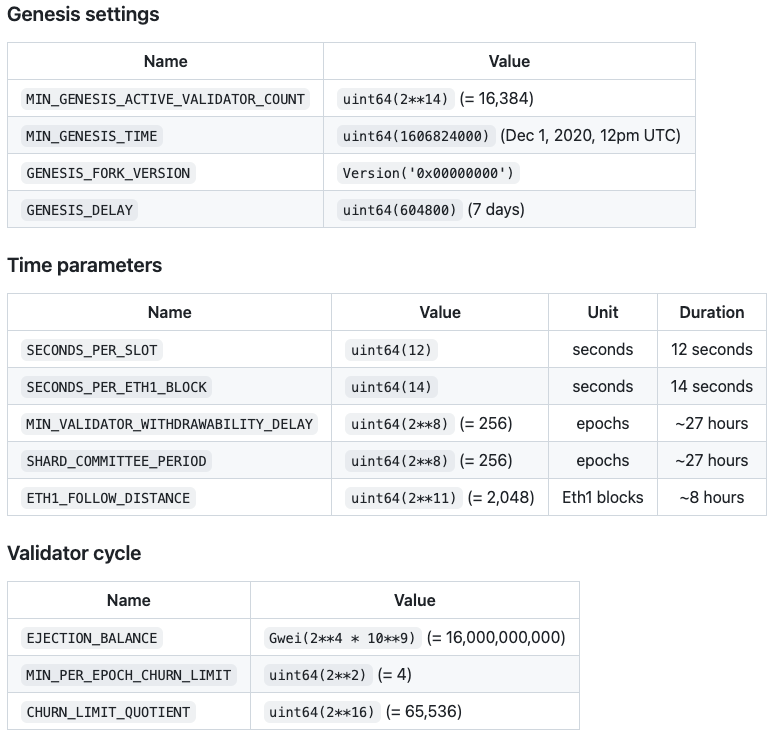
\includegraphics[width=0.9\linewidth]{images/configvalues}
\caption{Configuration settings}
\label{fig:config}
\end{center}
\end{figure}

\begin{figure}[htbp]
\begin{center}
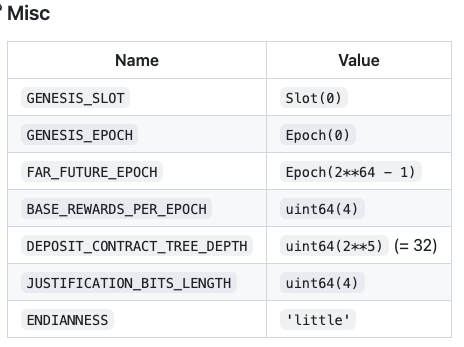
\includegraphics[width=0.4\linewidth]{images/constants}
\caption{Miscellaneous key constant values}
\label{fig:constants}
\end{center}
\end{figure}

\begin{figure}[htbp]
\begin{center}
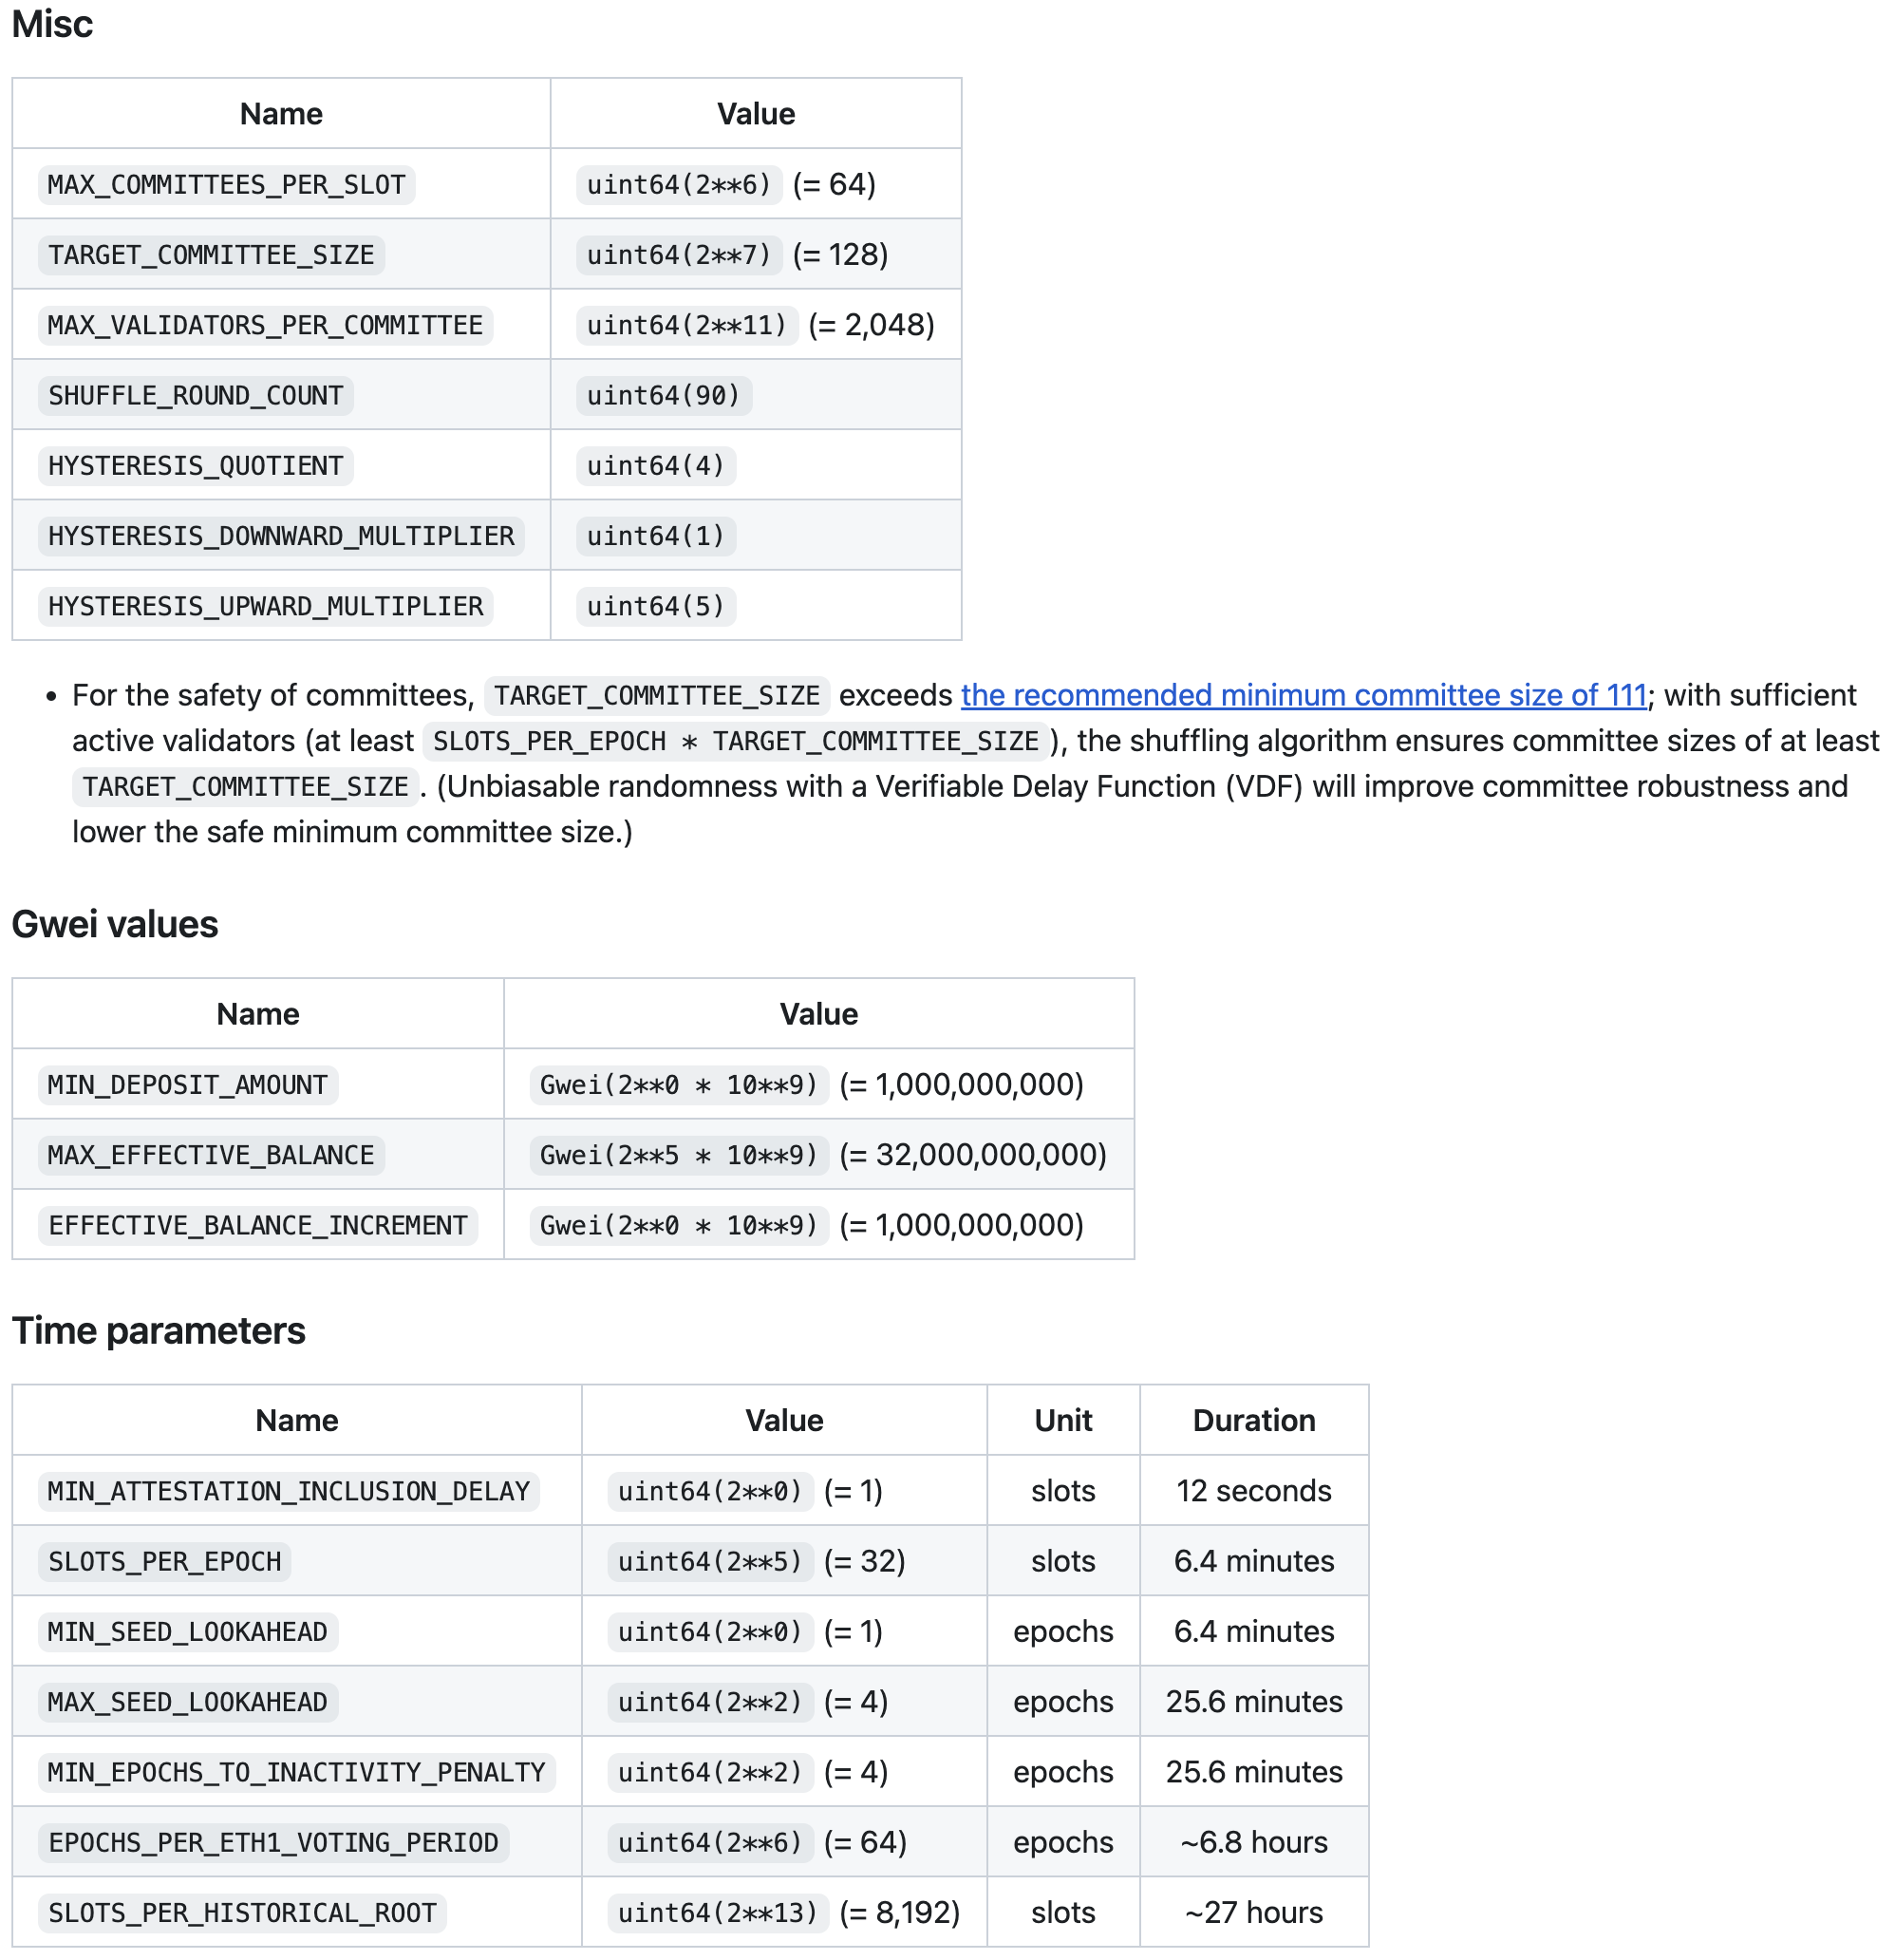
\includegraphics[width=0.9\linewidth]{images/committee}
\caption{Parameters for committees and time}
\label{fig:committee}
\end{center}
\end{figure}

 \begin{figure}[htbp]
\begin{center}
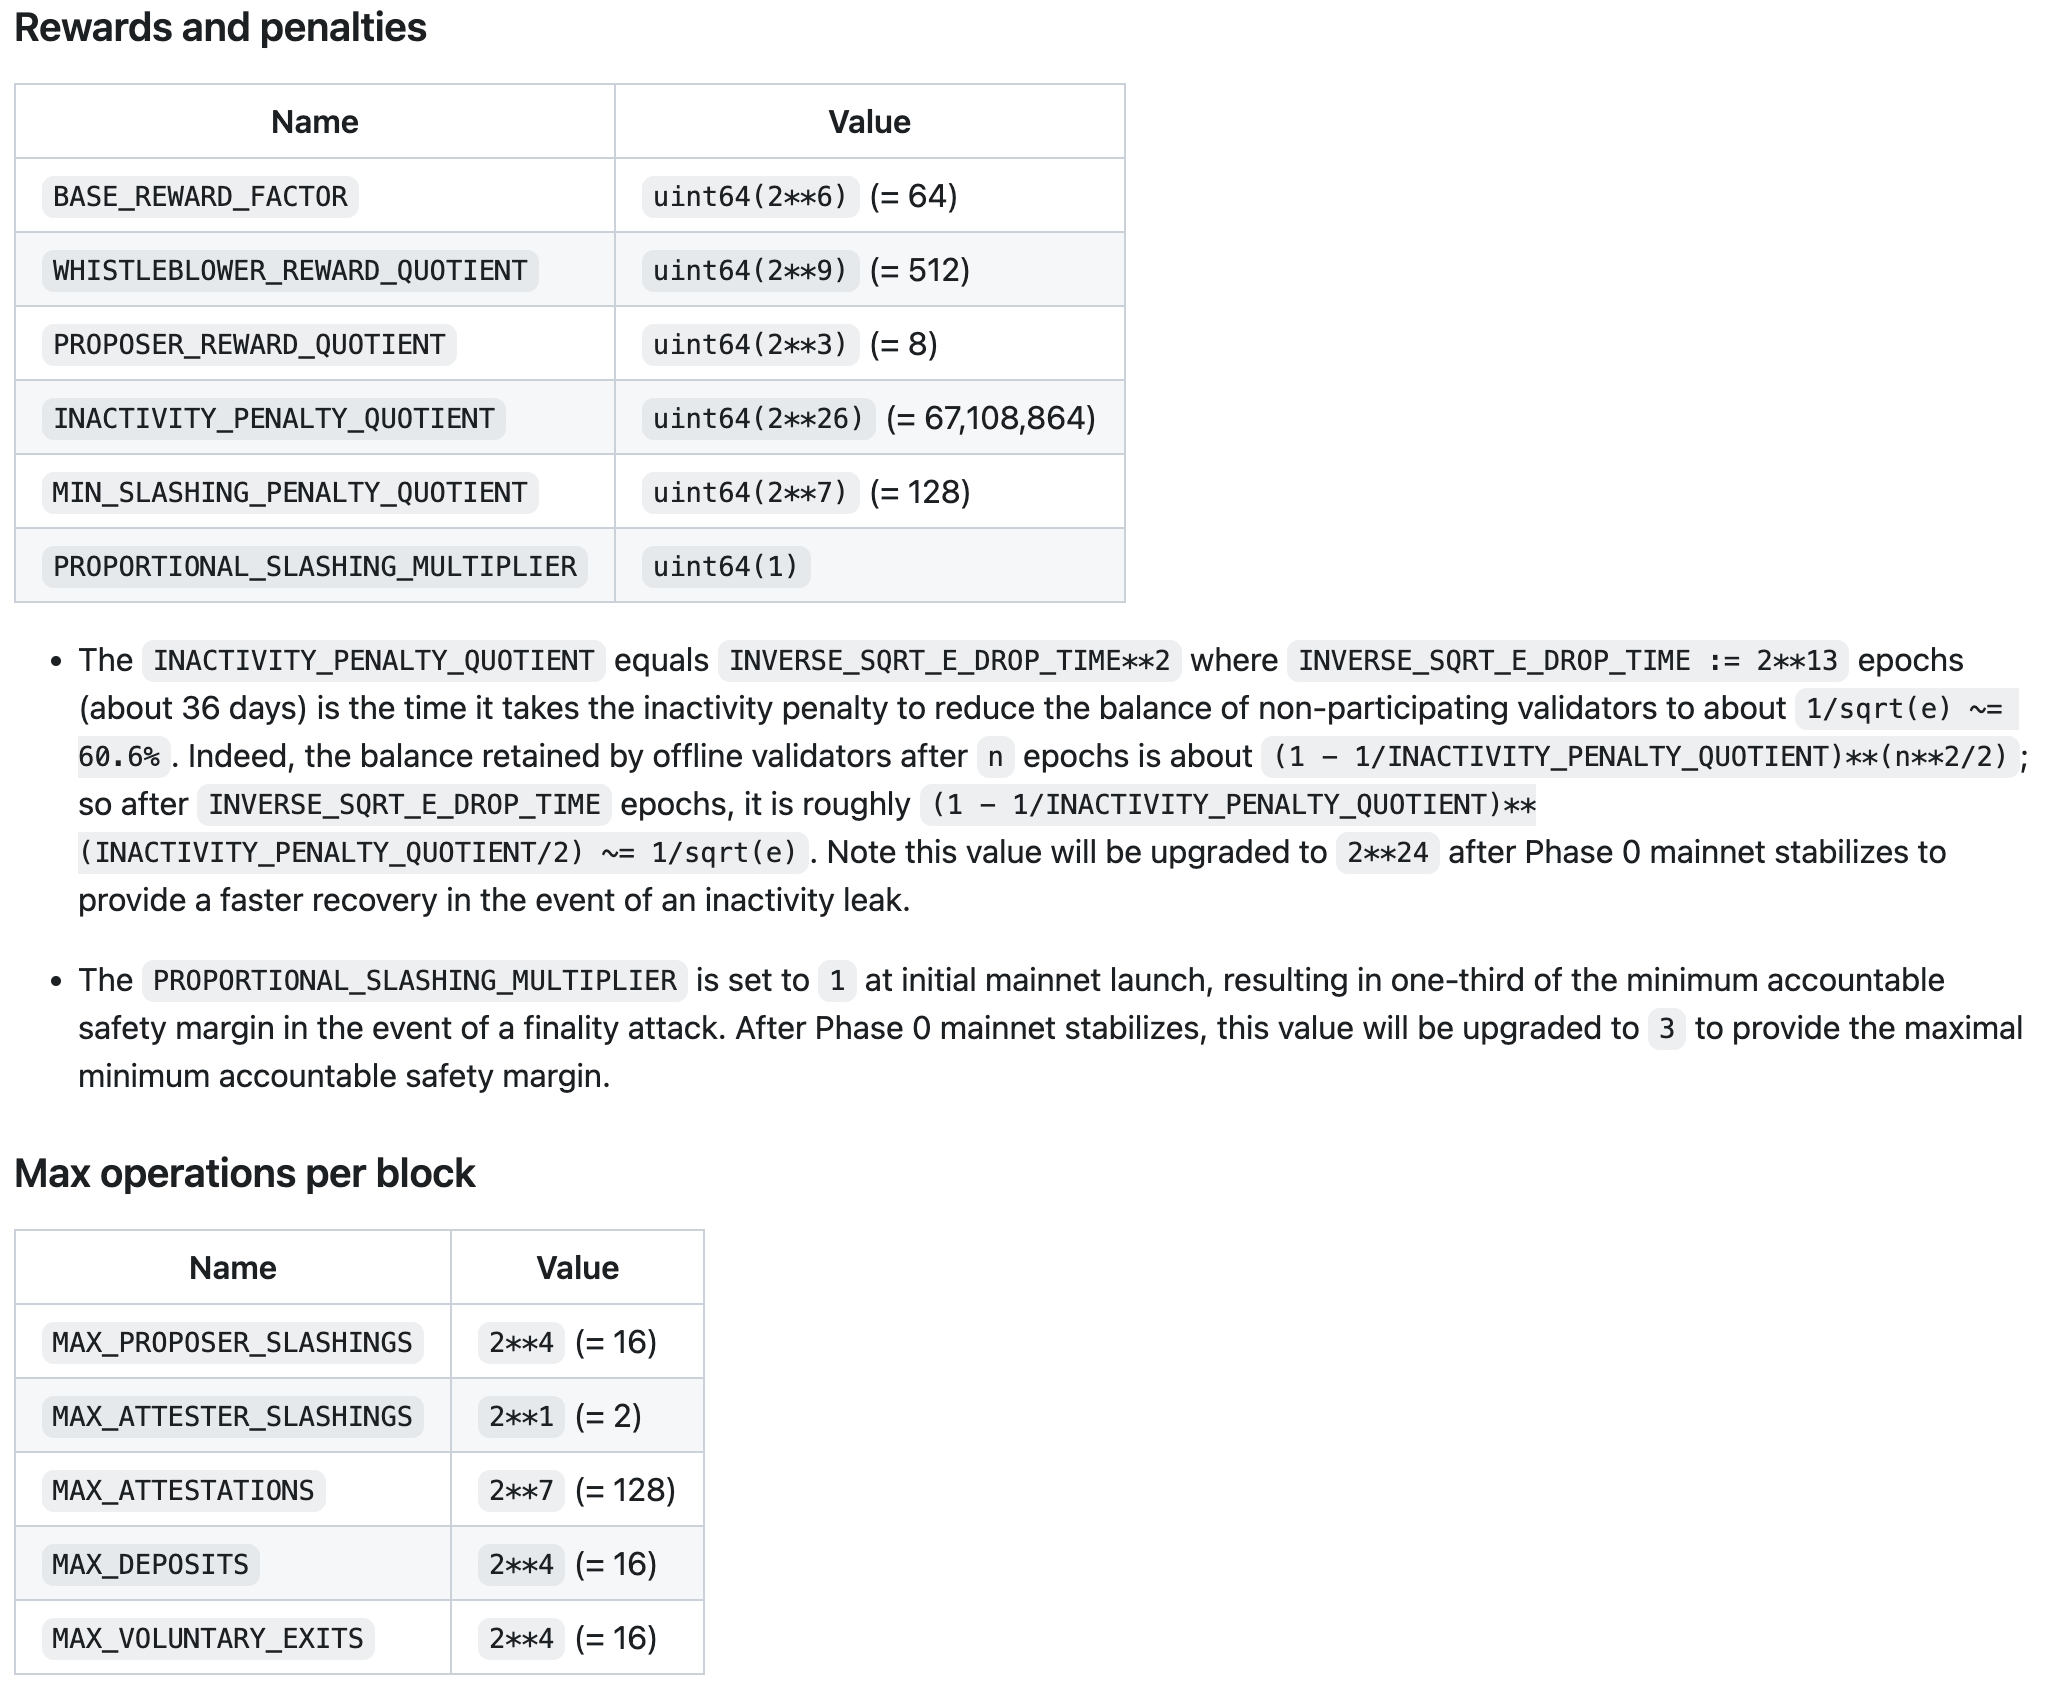
\includegraphics[width=\linewidth]{images/rewards}
\caption{Parameters for rewards and penalties, and operations}
\label{fig:rewards}
\end{center}
\end{figure}

Rocket Pool has a simple explanation of the various validator rewards and a table which summarises the expected rewards when staking: \href{https://docs.rocketpool.net/guides/node/responsibilities.html}{A Node Operator's Responsibilities}.
\clearpage
% ---------------------------------------------------------
 \subsection{Total ETH Supply}
 % ---------------------------------------------------------
\label{sec:ethsupply} 
        The total supply of ETH used to be fairly simple to work out, but it is now more complicated for two main reasons:  implementation of EIP-1559 and the Merge.
Currently we are ``(a) burning ETH via the base fee and (b) the issuance is variable depending on the number of validators.'' (Ben Edgington 2023). 
\begin{itemize}
	\item Ultrasound is considered a credible source for total ETH supply projections. \\\textit{\href{https://ultrasound.money/}{Ultra sound money}} visualises various aspects of Ether supply since the Merge, gas, supply projections, the burn, total value secured - TVS and monetary premium. See figures~\ref{fig:ethsupply}~-~\ref{fig:monetary}, on pages~\pageref{fig:ethsupply}~-~\pageref{fig:monetary}.  

\begin{itemize}
	\item Ultrasound supplied two datasets for our analysis - the first had total supply at a more accurate and finer grained level, but shorter time period and the second dataset had data points roughly every 1,000 epochs covering from soon after Beacon chain genesis. The latter dataset is from Glassnode and would not be as accurate as the initial data provided by Alex Tesfamichael from Ultrasound.
\end{itemize}
	\item \textit{\href{https://etherscan.io/chart/ethersupplygrowth}{Etherscan}} is a good source of historic data for the growth in Ether supply since 2015. There are several pages of detailed information and the \textit{Charts \& Statistics} webpage has several visualisations, often with the ability to select different time ranges and a link to download the raw data as csv files, providing that Etherscan is acknowledged when these datasets are used.\\
	Figures~\ref{fig:ethscan}~to~\ref{fig:ethgrowth} on pages~\pageref{fig:ethscan}~to~\pageref{fig:ethgrowth} show the visualisations that are currently available.
\end{itemize}

% -----------------------------------------------------------------
\subsection{Validators, Stakers and Staking pools}
% -----------------------------------------------------------------
\label{sec:stakers}
There are several helpful documents explaining in detail the different options available for staking:
\begin{itemize}
\item \href{https://ethereum.org/en/staking/solo/}{Solo staking}
\item \href{https://ethereum.org/en/staking/saas/}{Staking as a Service (Saas)}
\item \href{https://ethereum.org/en/staking/pools/}{Pooled staking}
\end{itemize}

The Ethereum Foundation and EtherScan conducted a survey of stakers \cite{Smith2023}, according to the following categories: solo staking, staking pool service, mini node operator (Rocketpool), and those not yet staking. The responses were analysed and the key trends, take aways, and predictions reported. The large majority of the respondents were either solo stakers or mini pool operators.


According to the \href{https://launchpad.ethereum.org/en/}{Staking Launchpad} on June 2023:
\begin{itemize}
\item Total ETH staked: 19,357,605 ETH
\item Total validators: 606,947
\item Current \gls{apr}: 4.74\%
\end{itemize}

\subsubsection*{LIDO}
% ----------------------------
LIDO is a popular liquid staking pool. 
At the time of writing, 7 June 2023, the total amount of ETH staked with \href{https://lido.fi/ethereum}{LIDO}  is 7,127,430 ETH. 

Several graphs have been generated in Dune Analytics. See Figures~\ref{fig:dunelido1}~to~\ref{fig:dunelido5} on pages~\pageref{fig:dunelido1}~to~\pageref{fig:dunelido5}.


\subsubsection*{Rocket Pool}
% -----------------------------------
A \href{https://rocketpool.net/}{Rocket Pool} node only needs to stake 16 ETH, and this stake is then coupled with 16 ETH from the staking pool to create a validator, known as a ``minipool''.  Staking in the Rocket Pool can be a stake of a little as 0.01 ETH, which is then issued as an rETH token representing the amount deposited into the pool. A node operator would obtain staked ETH from the pool to form a validator.

There is documentation at the Rocket Pool website that clearly explains Ethereum staking and how it works when staking with Rocket Pool.

Currently, 8 June 2023, Rocket Pool has staked 722,176 ETH and has 2,842 node operators.

If we can identify the number of distinct rETH token holders, we would be able to determine the number of stakers staking ETH in Rocket Pool. 
Examples of the graphs and information available from the Dune dashboard are shown in figures~\ref{fig:dunerocket1}~-~\ref{fig:rocketdrworm12} on pages~\pageref{fig:dunerocket1}~-~\pageref{fig:rocketdrworm12}.

\subsubsection*{Data from an archive node}
% --------------------------------------------------------
Accessing a teku-besu archive node, \texttt{teku-besu-ohio-mainnet-archive-01},  we were able to use several API endpints to extract some rich data for validators.\\
	 We selected several API endpoints from those listed in GitHub: \href{https://ethereum.github.io/beacon-APIs/?urls.primaryName=dev}{Eth Beacon Node API}\\
	 Some visualisations of validator information from the archive node are in figures~\ref{fig:dailyvalidator1}~-~\ref{fig:cumulativevalidatorsregression}, pages~\pageref{fig:dailyvalidator1}~-~\pageref{fig:cumulativevalidatorsregression}.
	 
\subsubsection*{Rated network explorer}
% --------------------------------------------------------	 
Rated provides \href{https://docs.rated.network}{documentation} for context and detail of the metrics and visualisations presented on its website.
	 The home page displays Beacon Chain validator ratings for the Ethereum beacon chain, figure~\ref{fig:ratedentity1}, page~\pageref{fig:ratedentity1}, but one can also select the G\"oerli test network to display ratings for those validators.
Figure~\ref{fig:ratednw1}, page~\pageref{fig:ratednw1} depicts four metrics to reflect network health and four reference rates of return for the entire active validator set.


% ----------------------------------------------------------
\subsection{Client and staking pool diversity}
% ---------------------------------------------------------
\label{sec:diversity}
\begin{itemize}
	\item \textit{\href{https://clientdiversity.org/}{Diversify Now}} dashboard by \textit{\href{https://etheralpha.org/}{Ether alpha}} displays the current client distribution in the Consensus and Execution layers. (Figure~\ref{fig:CLELdiversity}, page~\pageref{fig:CLELdiversity}).
	\item \textit{\href{https://migalabs.es/beaconnodes}{Beacon Chain Network Public Dashboard}} by \textit{\href{https://migalabs.es/}{Miga Labs}} has several visualisations: 
	\begin{itemize}
		\item Client diversity  (Figure~\ref{fig:diversity}(a), page~\pageref{fig:diversity})
		\item Client diversity evolution (Beacon chain client distribution over time) (Figure~\ref{fig:diversity}(b), page~\pageref{fig:diversity})
		\item OS distribution of active nodes (Figure~\ref{fig:active}(a), page~\pageref{fig:active})
		\item Geographical representation of client evolution over time  (Figure~\ref{fig:active}(b), page~\pageref{fig:active})
		\item Active nodes round trip time distribution (RTT) (Figure~\ref{fig:rtt}(a), page~\pageref{fig:rtt})
		\item Graphical distribution (Beacon chain node distribution)  (Figure~\ref{fig:rtt}(b), page~\pageref{fig:rtt})
		\item RTT distribution (Figure~\ref{fig:aass}(a), page~\pageref{fig:aass})
		\item Advertised attestation subnets subscription (Figure~\ref{fig:aass}(b), page~\pageref{fig:aass})
		\item Number of beach nodes per IP (Figure~\ref{fig:ipdist}), page~\pageref{fig:ipdist})
	\end{itemize}
However, it is important to note that it is challenging to measure peer types in the network, and therefore the figures are at best approximations based on the information at hand. 

\end{itemize}	


% ---------------------------------------------------------	
\subsection{Multiple datasets}
% ---------------------------------------------------------
There are several resources that contain lists and visualisations of a variety of data from Ethereum Mainnet. Obtaining the raw data used on the websites and dashboards are not always easily accessible.
\label{sec:multiple}
\begin{itemize}
	\item \textit{\href{https://beaconcha.in/}{beaconcha.in}}, an open source Ethereum explorer, is a rich and informative resource providing visualisations and summary statistics of various aspects of the chain. It is not clear if it is possible to gain access to the data used to generate the many graphs and summary statistics. The website currently contains the following:
	\begin{itemize}
		\item On the home page, there is a \textbf{progress line} at the top of the page showing the \textit{number of slots left in the current epoch}. (Figure~\ref{fig:bhomepg}, page~\pageref{fig:bhomepg})
		\item Immediately below the progress line, there is a \textbf{summary line} showing the \textit{current epoch number}, the \textit{last finalised epoch}, the \textit{current slot number}, the \textit{number of active and pending validators}, the \textit{total staked ETH} and the \textit{average validator balance}. (Figure~\ref{fig:bhomepg})
		\item Below this summary there is a \textbf{graph} of the \textit{number of active validators} and \textit{staked ETH} for the last week (Figure~\ref{fig:bhomepg})
		\item Then there are two side by side tables. The \textbf{left table} has information about the most recent epochs: \textit{epoch number, time, whether it is final, the eligible ETH, the number of percentage of votes}. The \textbf{right table} has information about the most recent blocks: \textit{epoch number, slot number, block number, status of the block (proposed or missed), time} and the \textit{proposer id}. These two tables are shown in Figure~\ref{fig:bhomepg2}, page~\pageref{fig:bhomepg2}).\\
		\item Moreover, one can click on the epoch, slot and block numbers in the tables to obtain a detailed view of the epoch, slot or block number. 
		\item There is also a link to the validator ID in the right table that provides a detailed view of that validator.
		\item Figures~\ref{fig:bepochs}~-~\ref{fig:bmempool} on pages~\pageref{fig:bepochs}~-~\pageref{fig:bmempool} displays detailed blockchain data.
		\item Figures~\ref{fig:bvalidators}~-~\ref{fig:bblschgs} on pages~\pageref{fig:bvalidators}~-~\pageref{fig:bblschgs} displays detailed validator data.
		\item Beaconcha.in provide additional visualisations and tools. For example, the ability to generate graphs to show the correlation between two variables (Figure~\ref{fig:bcorrelations} on page~\pageref{fig:bcorrelations}.
	\end{itemize}

	\item \textit{\href{https://mevboost.pics}{Mevboost.pics}} 
	\begin{itemize}
		\item \textit{\href{https://mevboost.pics}{MEV-Boost General Dashboard}}\\
		Examples of the contents displayed on the general dashboard can be seen in figures~\ref{fig:mevhome1}~-~\ref{fig:mevhome4} on pages~\pageref{fig:mevhome1}~-~\pageref{fig:mevhome4}.
		\item \textit{\href{https://mevboost.pics}{MEV-Boost Builders Dashboard}}\\
		Examples of the contents displayed on the builders dashboard can be seen in figures~\ref{fig:mevbuilder1}~-~\ref{fig:mevbuilder4} on pages~\pageref{fig:mevbuilder1}~-~\pageref{fig:mevbuilder4}.
		\item \textit{\href{https://mevboost.pics}{MEV-Boost Relays Dashboard}}\\
		Examples of the contents displayed on the relays dashboard can be seen in figures~\ref{fig:mevrelay1}~-~\ref{fig:mevrelay4} on pages~\pageref{fig:mevrelay1}~-~\pageref{fig:mevrelay4}.
		\item \textit{\href{https://mevboost.pics}{MEV-Boost Validators Dashboard}}\\
		Examples of the contents displayed on the validators dashboard can be seen in figures~\ref{fig:mevvalidator1}~-~\ref{fig:mevvalidator4} on pages~\pageref{fig:mevvalidator1}~-~\pageref{fig:mevvalidator4}.
		\item \textit{\href{https://mevboost.pics/data.html}{Mevboost.pics - Open Data}} will eventually provide links to download several datasets: (Figure~\ref{fig:mevboostrawdata}, page~\pageref{fig:mevboostrawdata})
		\begin{itemize} 
			\item \textit{eth\_data} - Slots since Merge with additional MEV-Boost and validator info such as: date, slot, block number, relay, builder pubkey, proposer pubkey, mevboost value, builder, validator \textit{(Available now)}
			\item \textit{pubkey\_mapping} - Validator public keys mapped to known entities such as Lido, Kraken ect. \textit{(Available now)}
			\item \textit{tc\_txs} - Tornado Cash related transactions \textit{(Not available)}
			\item \textit{staking\_txs} - Deposit transactions to the ETH2 Deposit contract \textit{(Not available)}
			\item \textit{relays\_over\_time} - Number of successfully relayed blocks per day \textit{(Not available)}
			\item \textit{builders\_over\_time} - Number of successfully built blocks per day \textit{(Not available)}
		\end{itemize}
	\end{itemize}
	\item \textit{\href{https://app.metrika.co/ethereum/}{Metrika}} \\
	The various dashboards available from Metrika are sponsored by the Ethereum Foundation. One can enter a withdrawal address in the search field on the homepage to retrieve withdrawal information for the time range selected, which is either 1 day, 1 week or 2 weeks. See figure~\ref{fig:metrika1} on page\pageref{fig:metrika1}. Following this there are several charts and tables covering the network, consensus, withdrawals and validators. Screen shots of the additional visualisations and tables are shown in figures~\ref{fig:metrika2}~-~\ref{fig:metrika6} on pages~\pageref{fig:metrika2}~-~\pageref{fig:metrika6}.

\end{itemize}

\clearpage

% ---------------------------------------------------------------
\subsection{Existing visualisations}
% --------------------------------------------------------------
\subsubsection*{Diversify Now}
% --------------------------------------
\begin{figure}[htbp]
\begin{center}
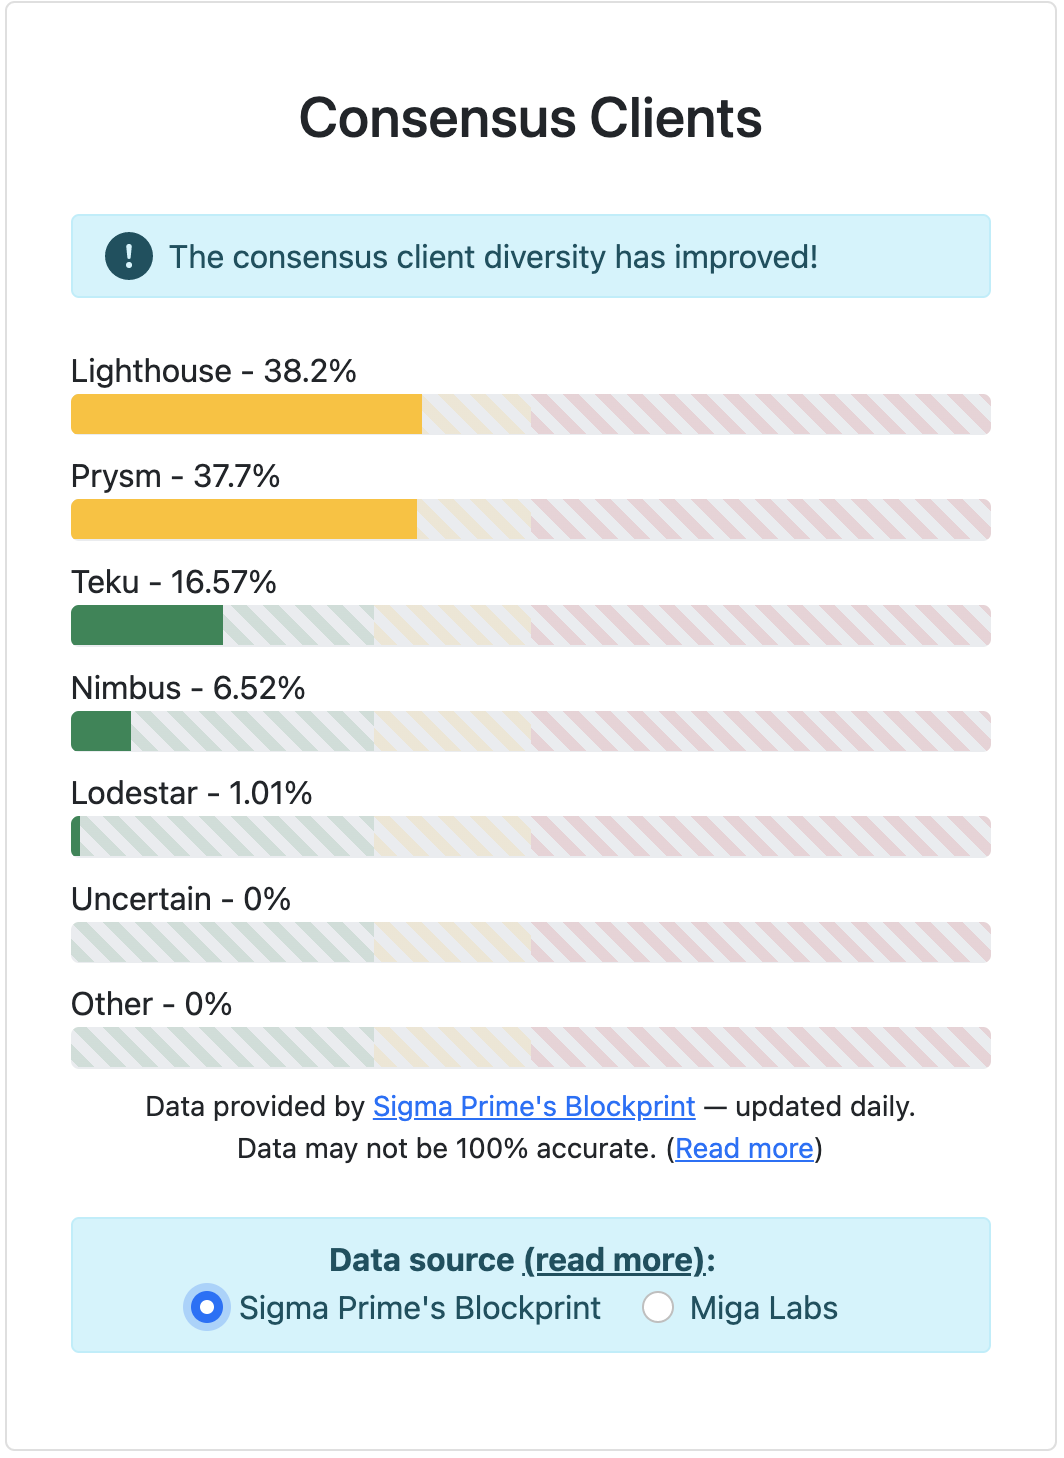
\includegraphics[width=0.3\linewidth, align=c]{images/CL-sigma}
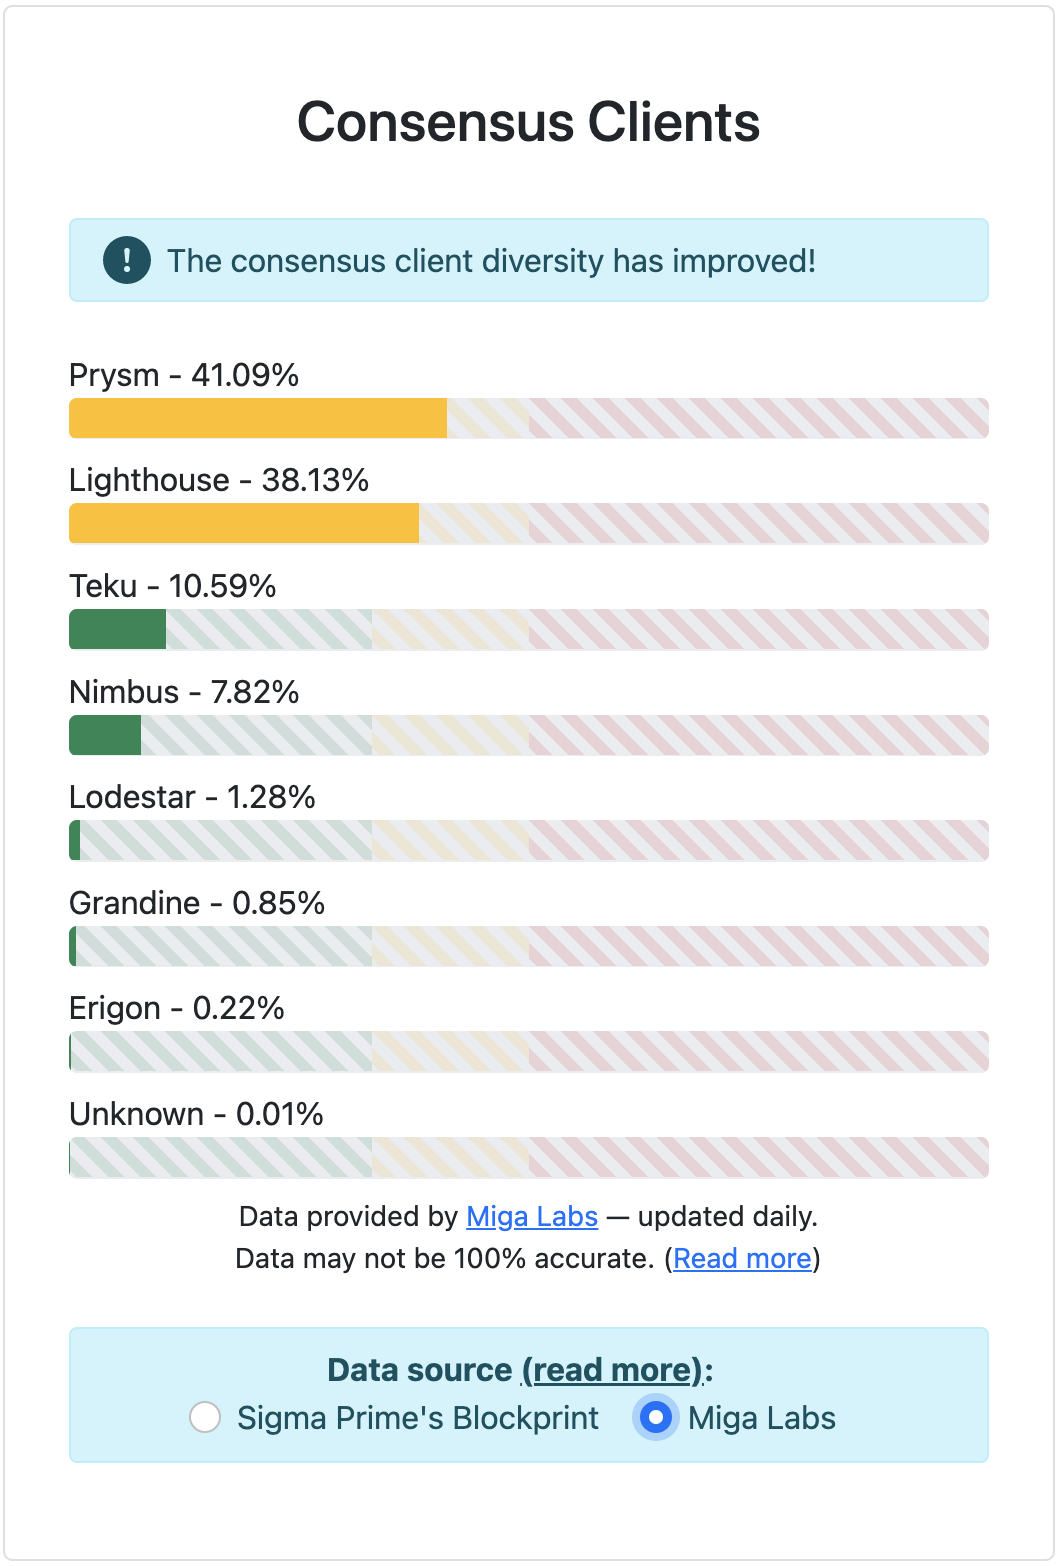
\includegraphics[width=0.3\linewidth, align=c]{images/CL-migalabs}
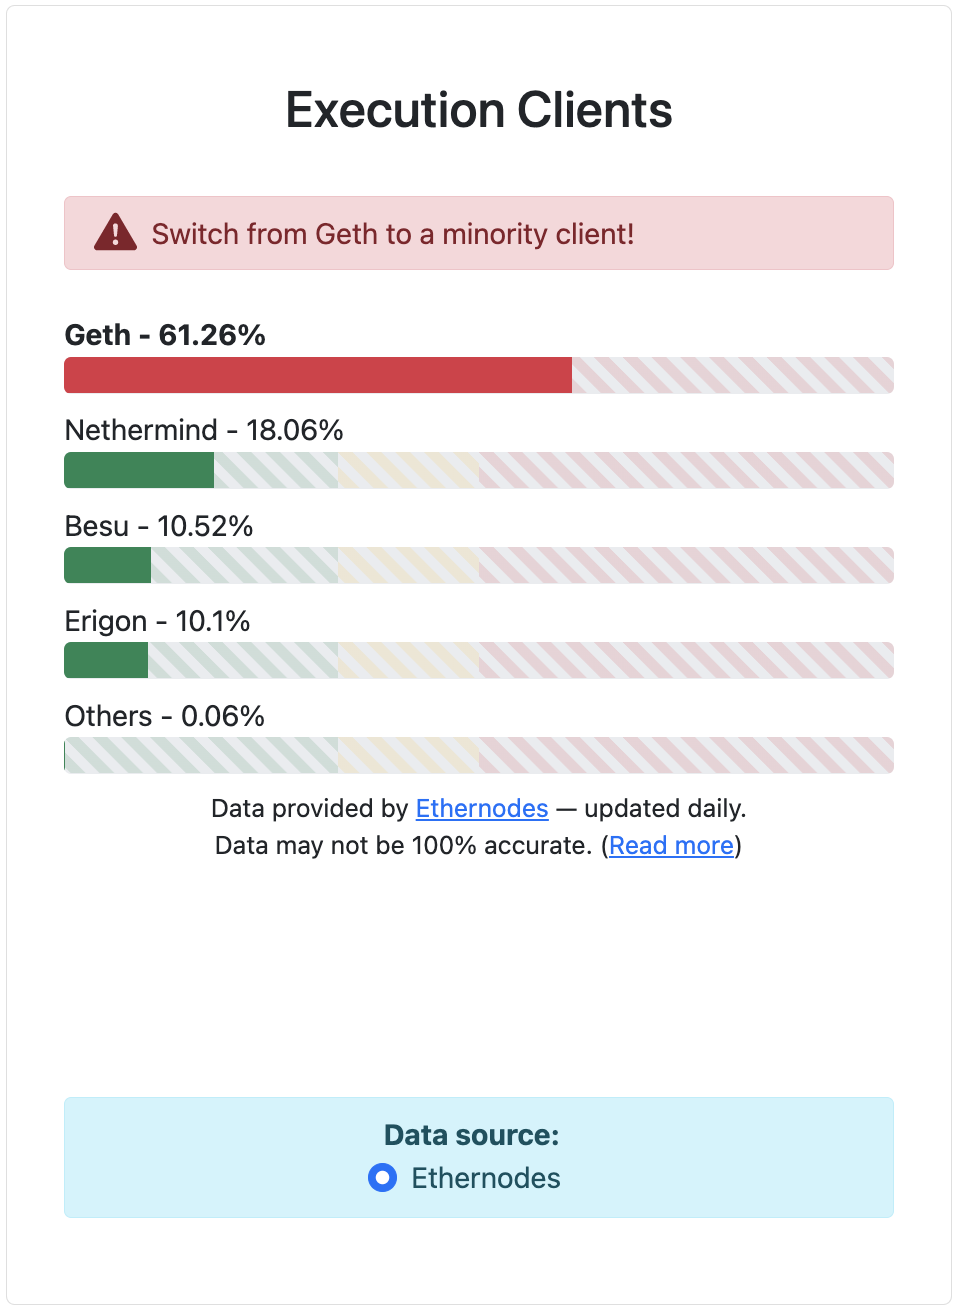
\includegraphics[width=0.3\linewidth, align=c]{images/EL-diversity}\\
(a)\hspace{110pt}        (b)\hspace{110pt} (c)\\
\caption{Consensus layer client diversity using Sigma Prime's Blockprint data (a) and using Migalabs data (b). Execution layer client diversity using Ethernodes data (19 May 2023)}
\label{fig:CLELdiversity}
\end{center}
\end{figure}
\clearpage
% --------------------------------------
\subsubsection*{Migalabs}
% --------------------------------------
 \begin{figure}[htbp]
\begin{center}
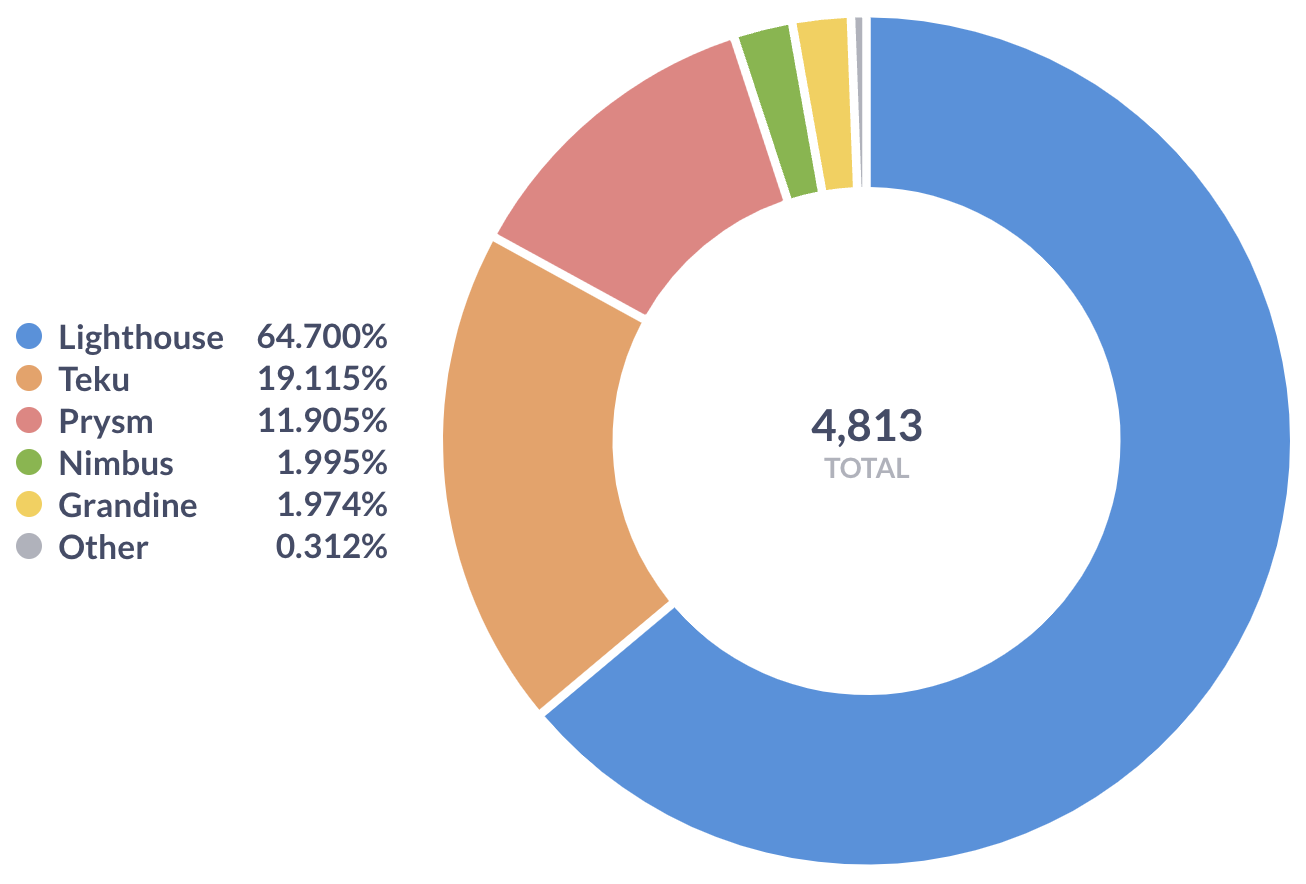
\includegraphics[width=0.48\linewidth]{images/clientdiversity}
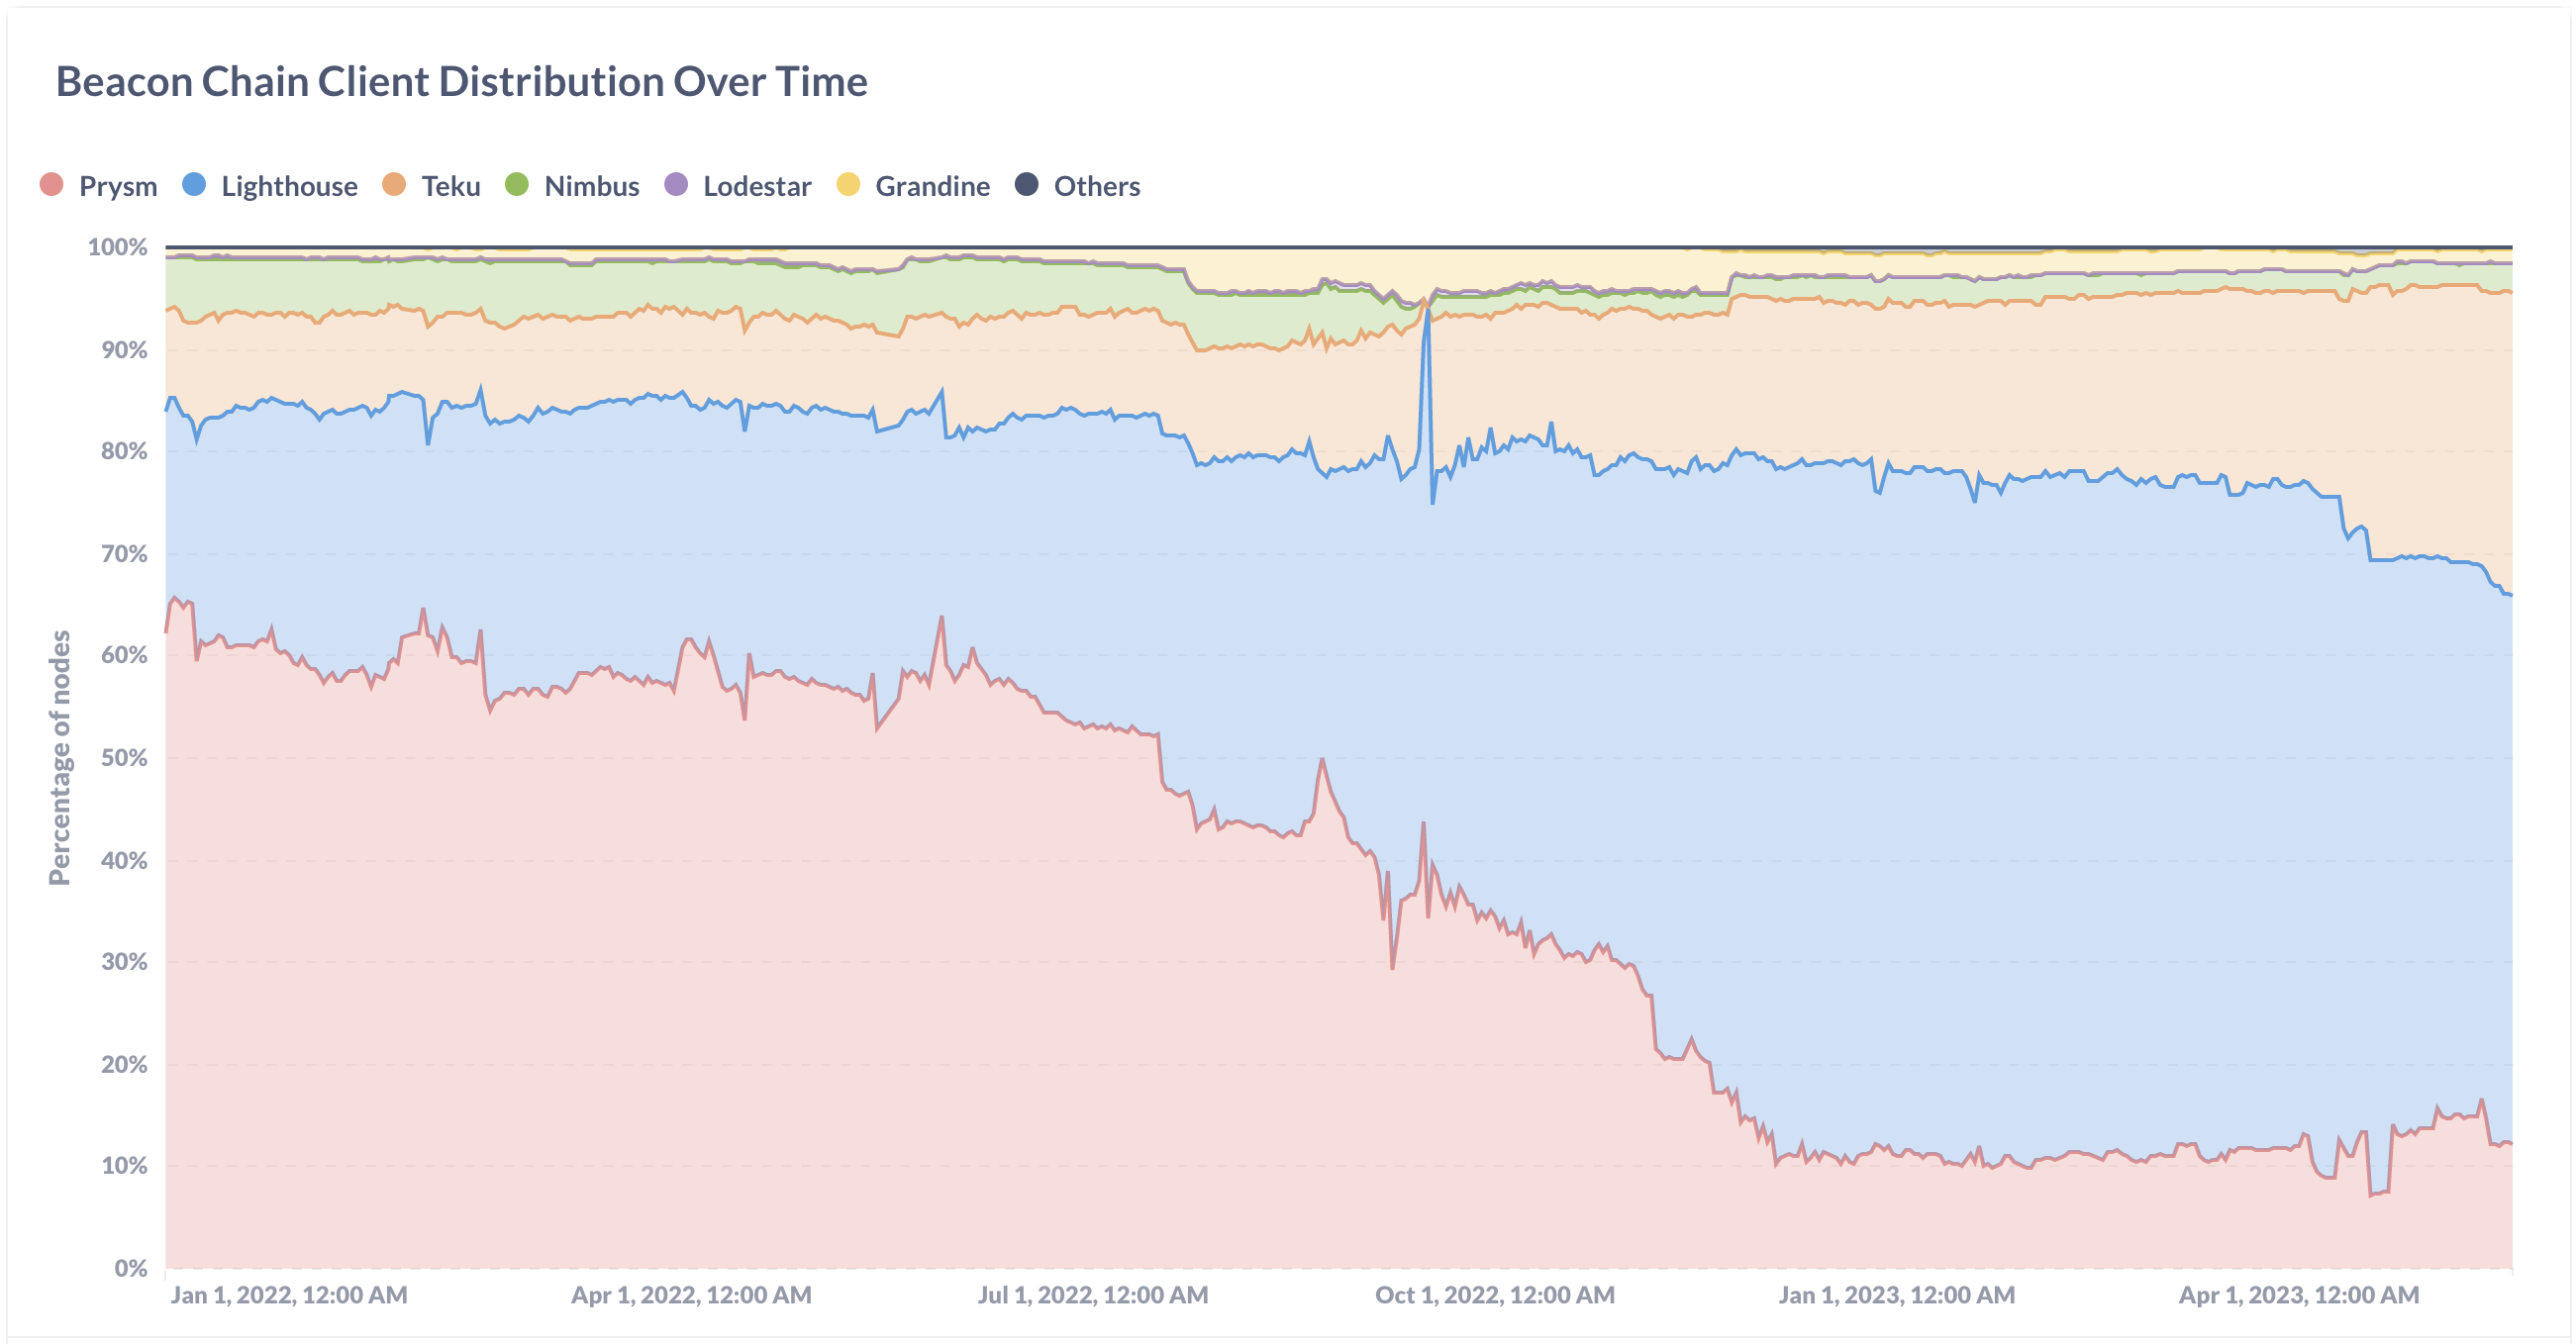
\includegraphics[width=0.48\linewidth]{images/architecture} \\
(a)\hspace{160pt}        (b)\\
\caption{Beacon chain client diversity from Migalabs (a) and client distribution over time (b) (9 May 2023)}
\label{fig:diversity}
\end{center}
\end{figure}

\begin{figure}[htbp]
\begin{center}
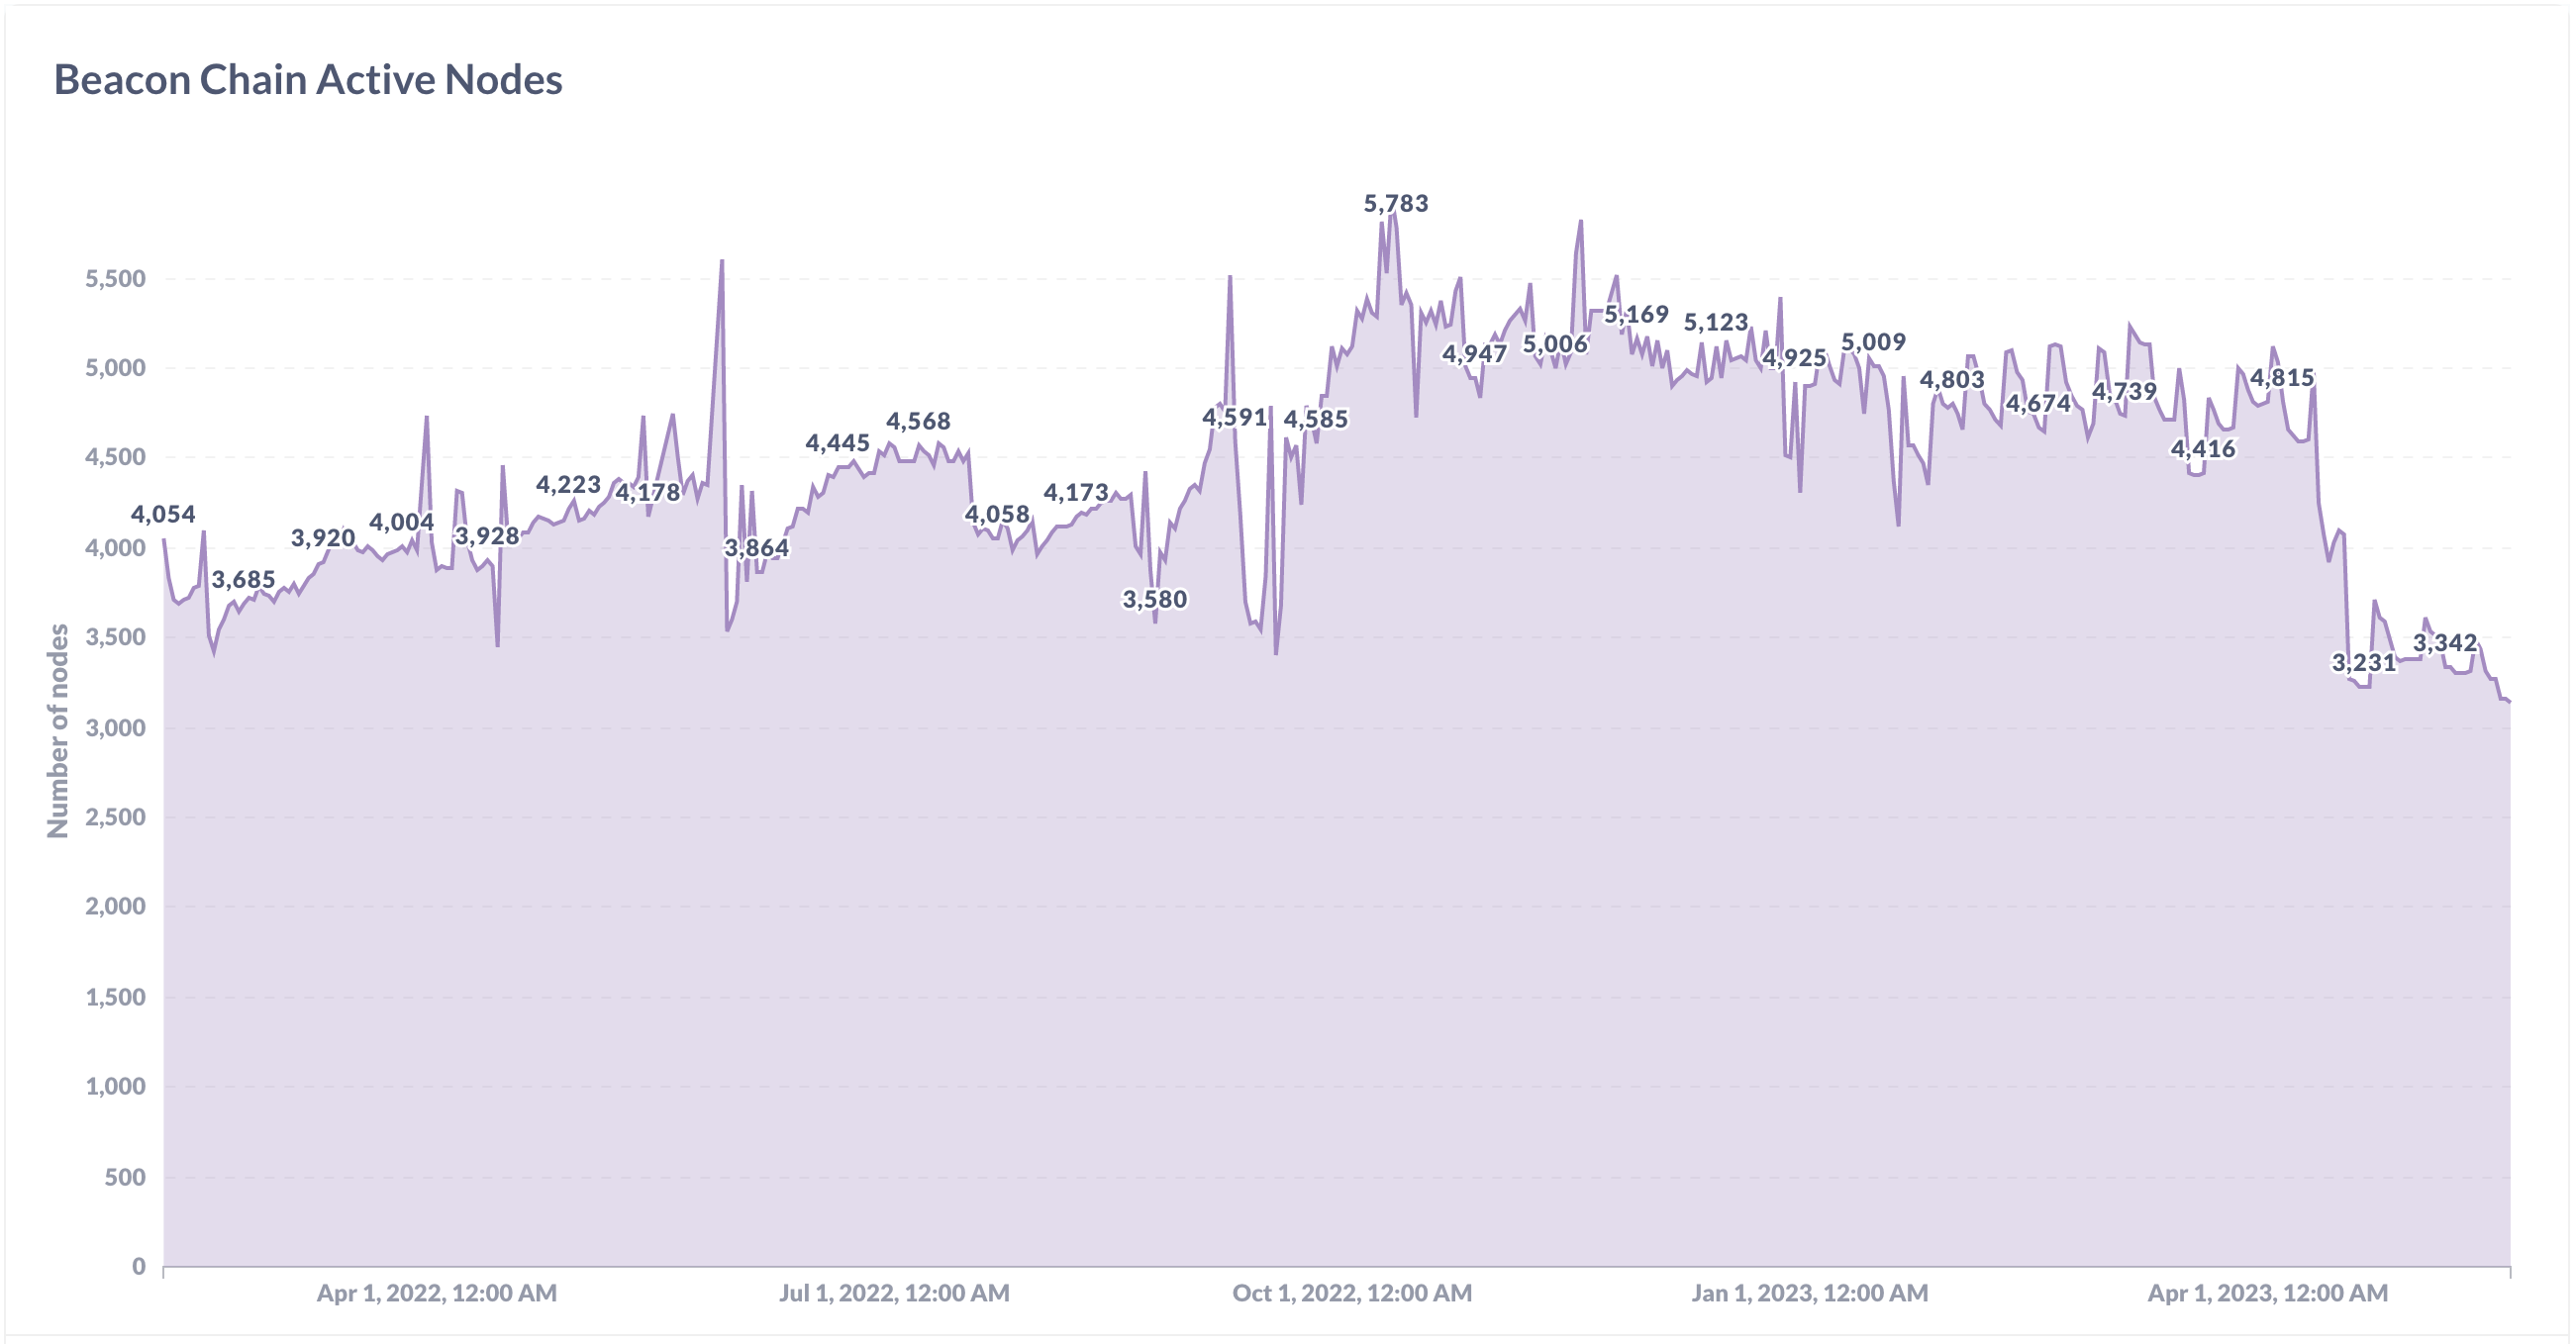
\includegraphics[width=0.48\linewidth]{images/activenodes}
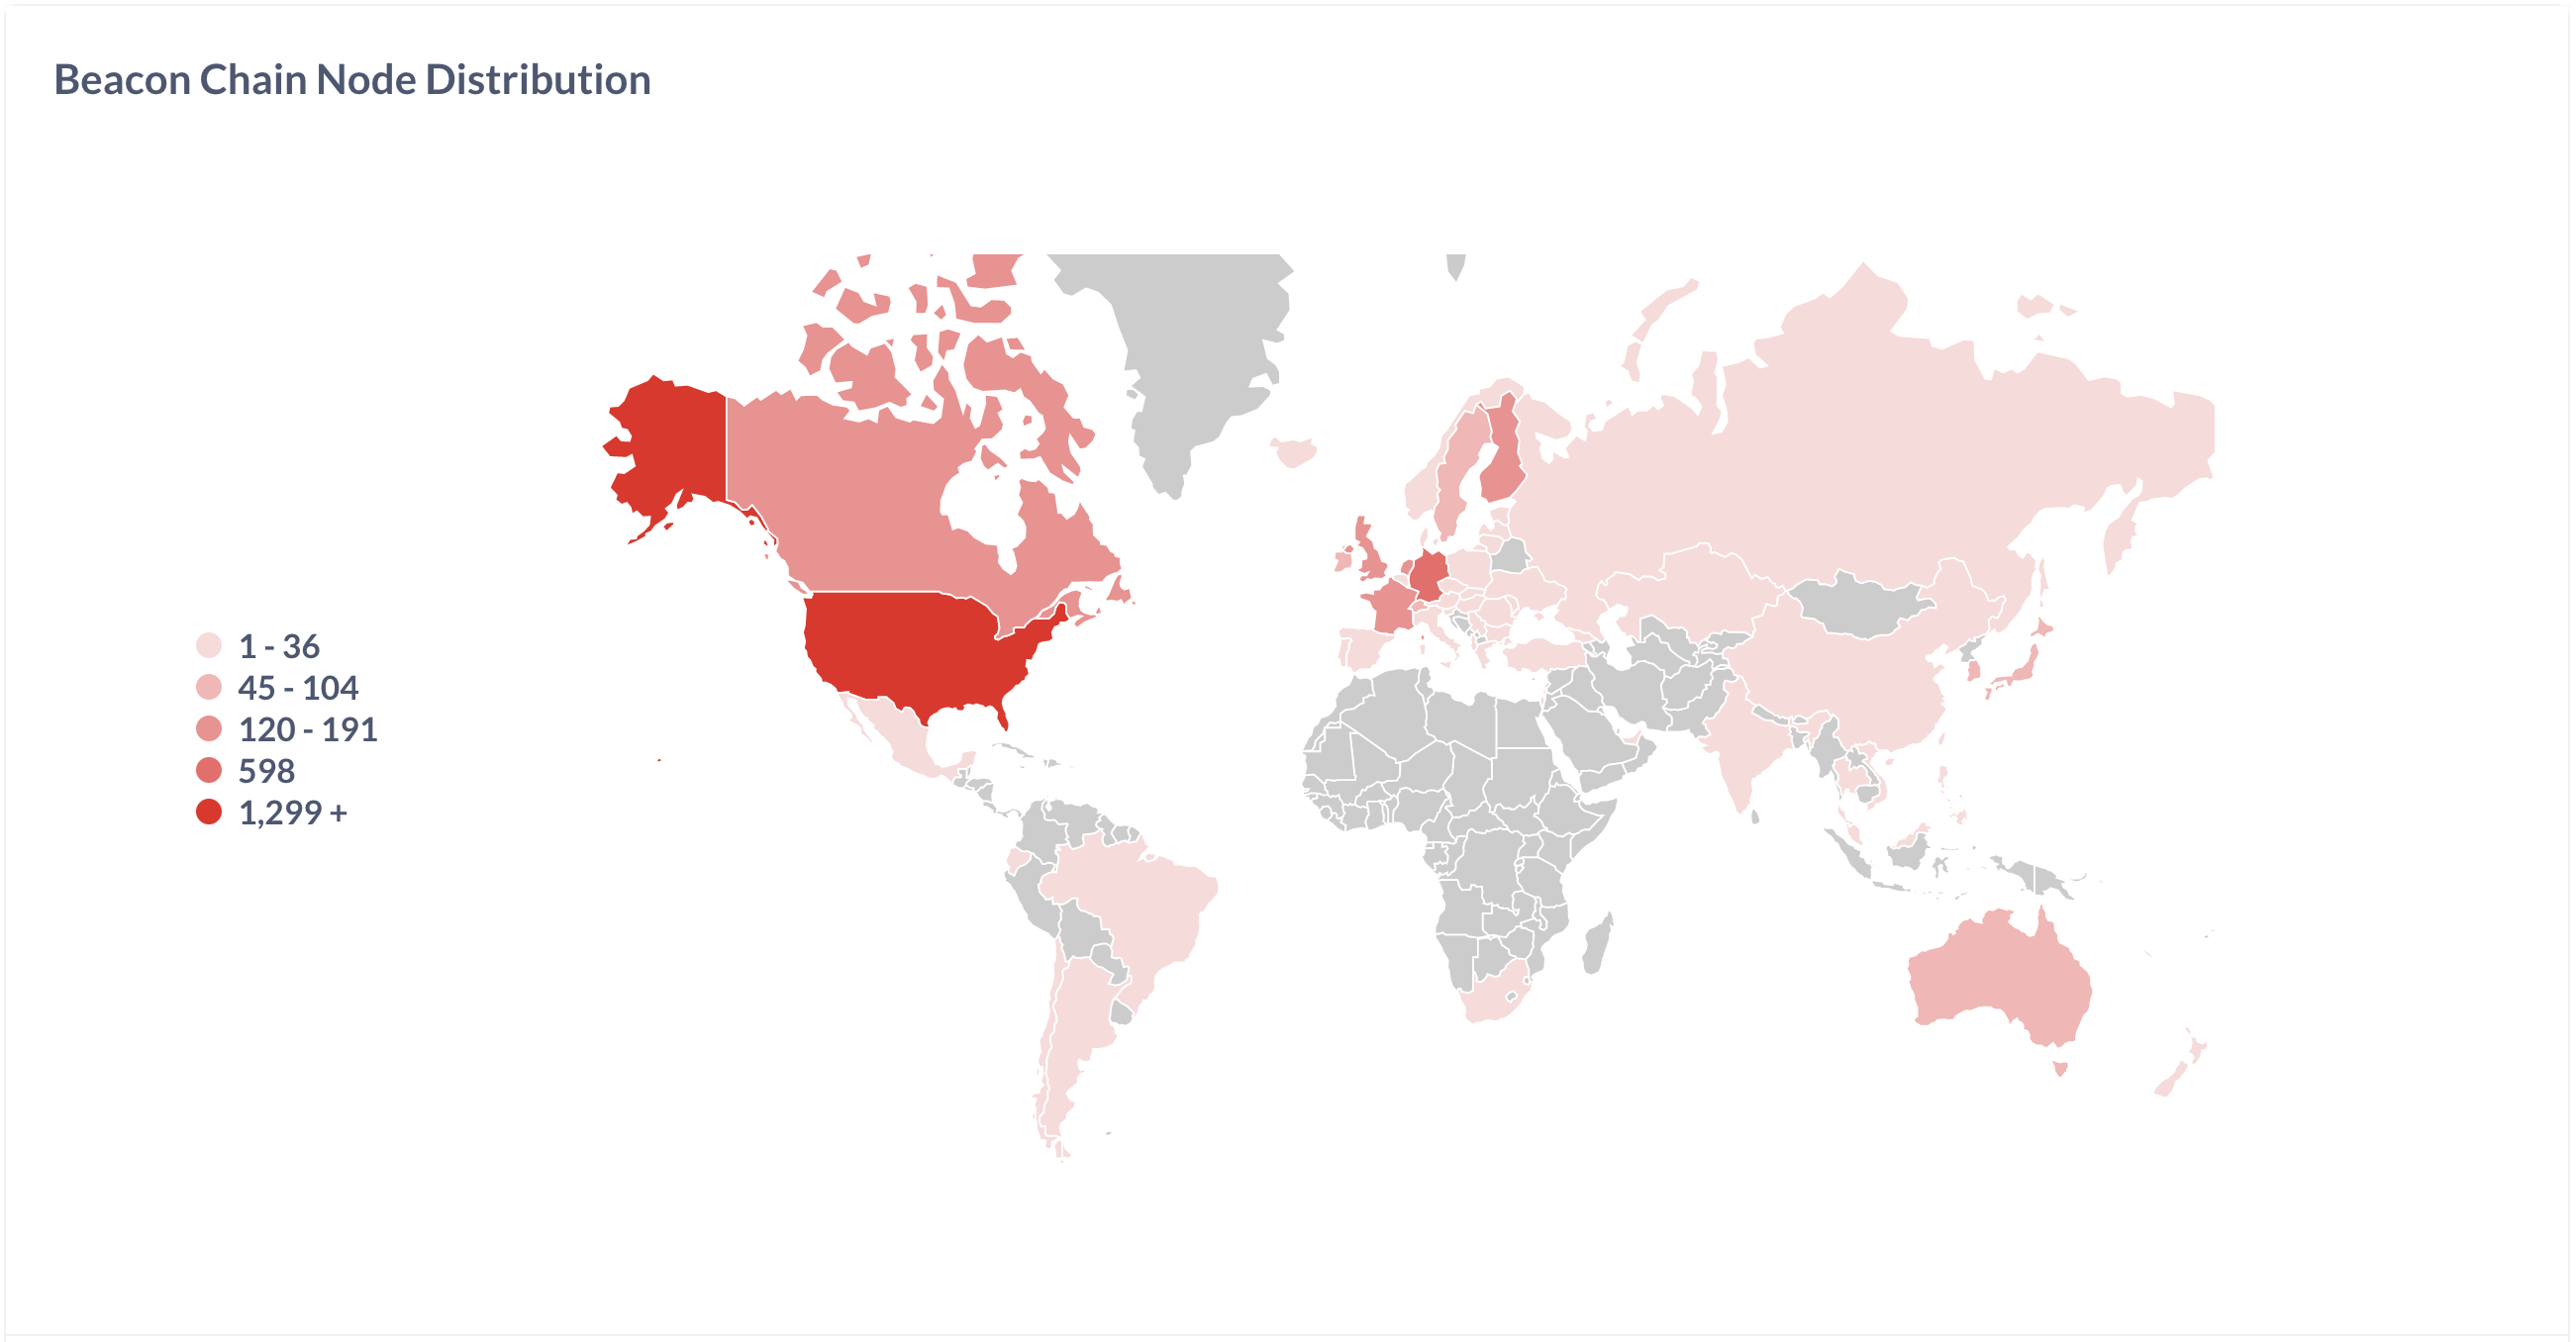
\includegraphics[width=0.48\linewidth]{images/evolution} \\
(a)\hspace{160pt}        (b)\\
\caption{Operating system distribution of active beacon chain nodes from Migalabs (a) and client diversity evolution of beacon chain nodes (b) (9 May 2023)}
\label{fig:active}
\end{center}
\end{figure}

\begin{figure}[htbp]
\begin{center}
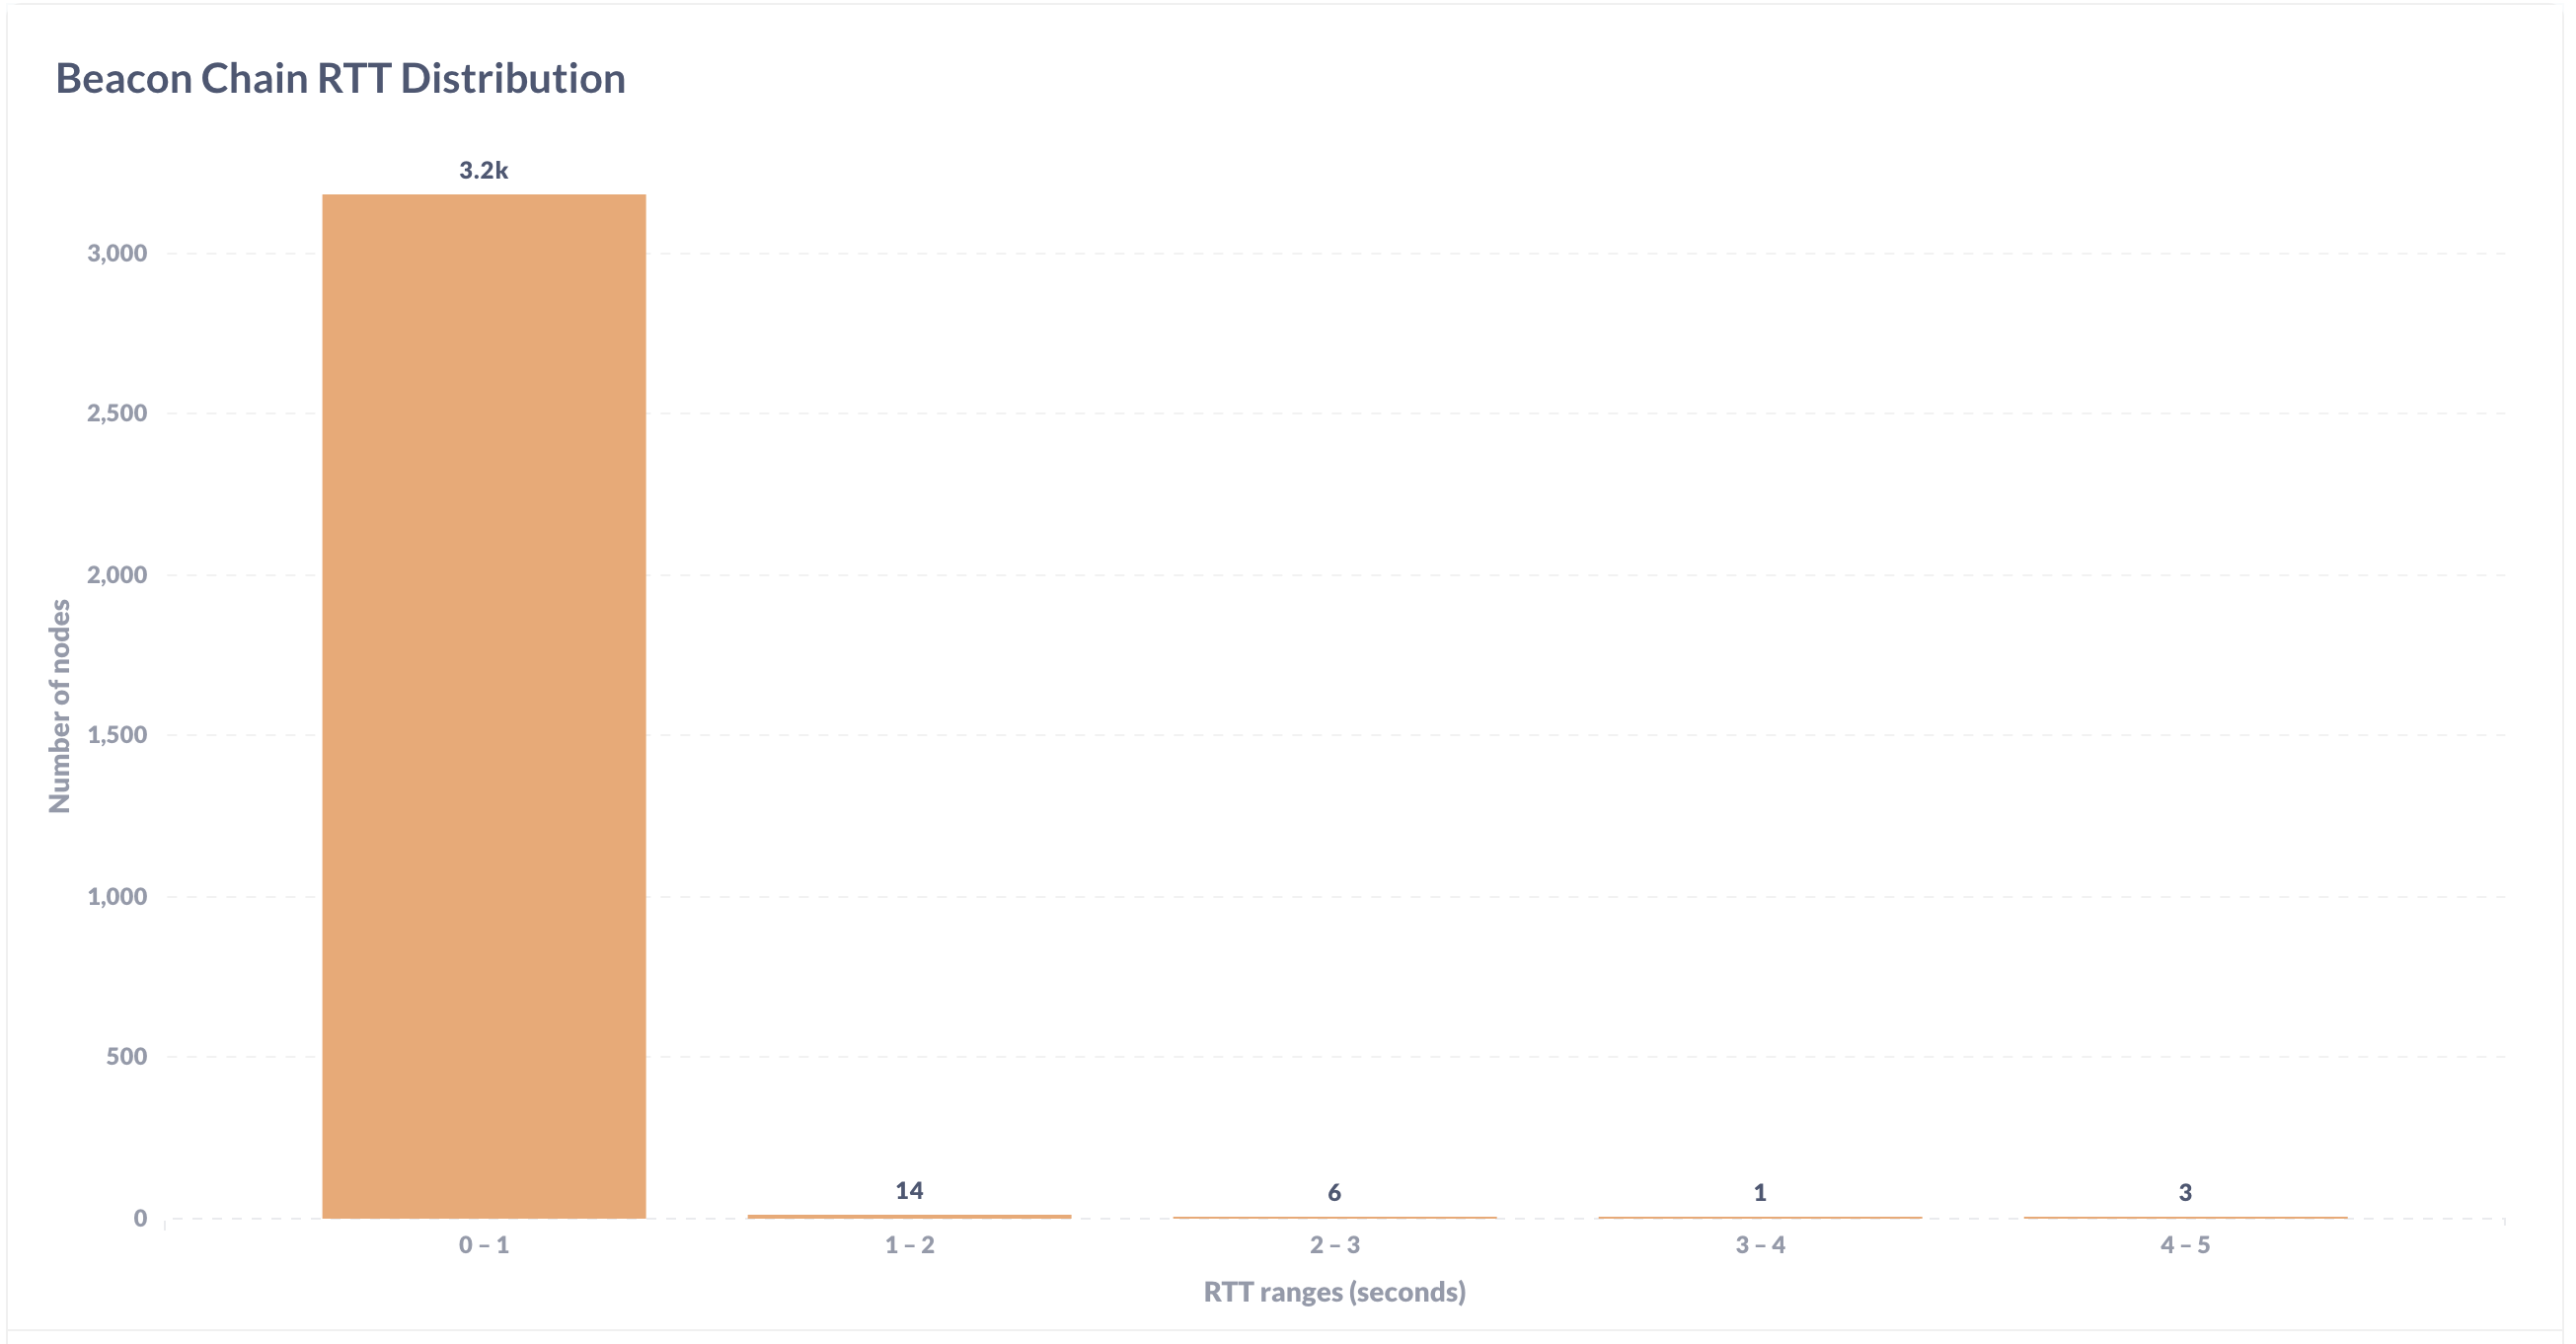
\includegraphics[width=0.48\linewidth]{images/activertt}
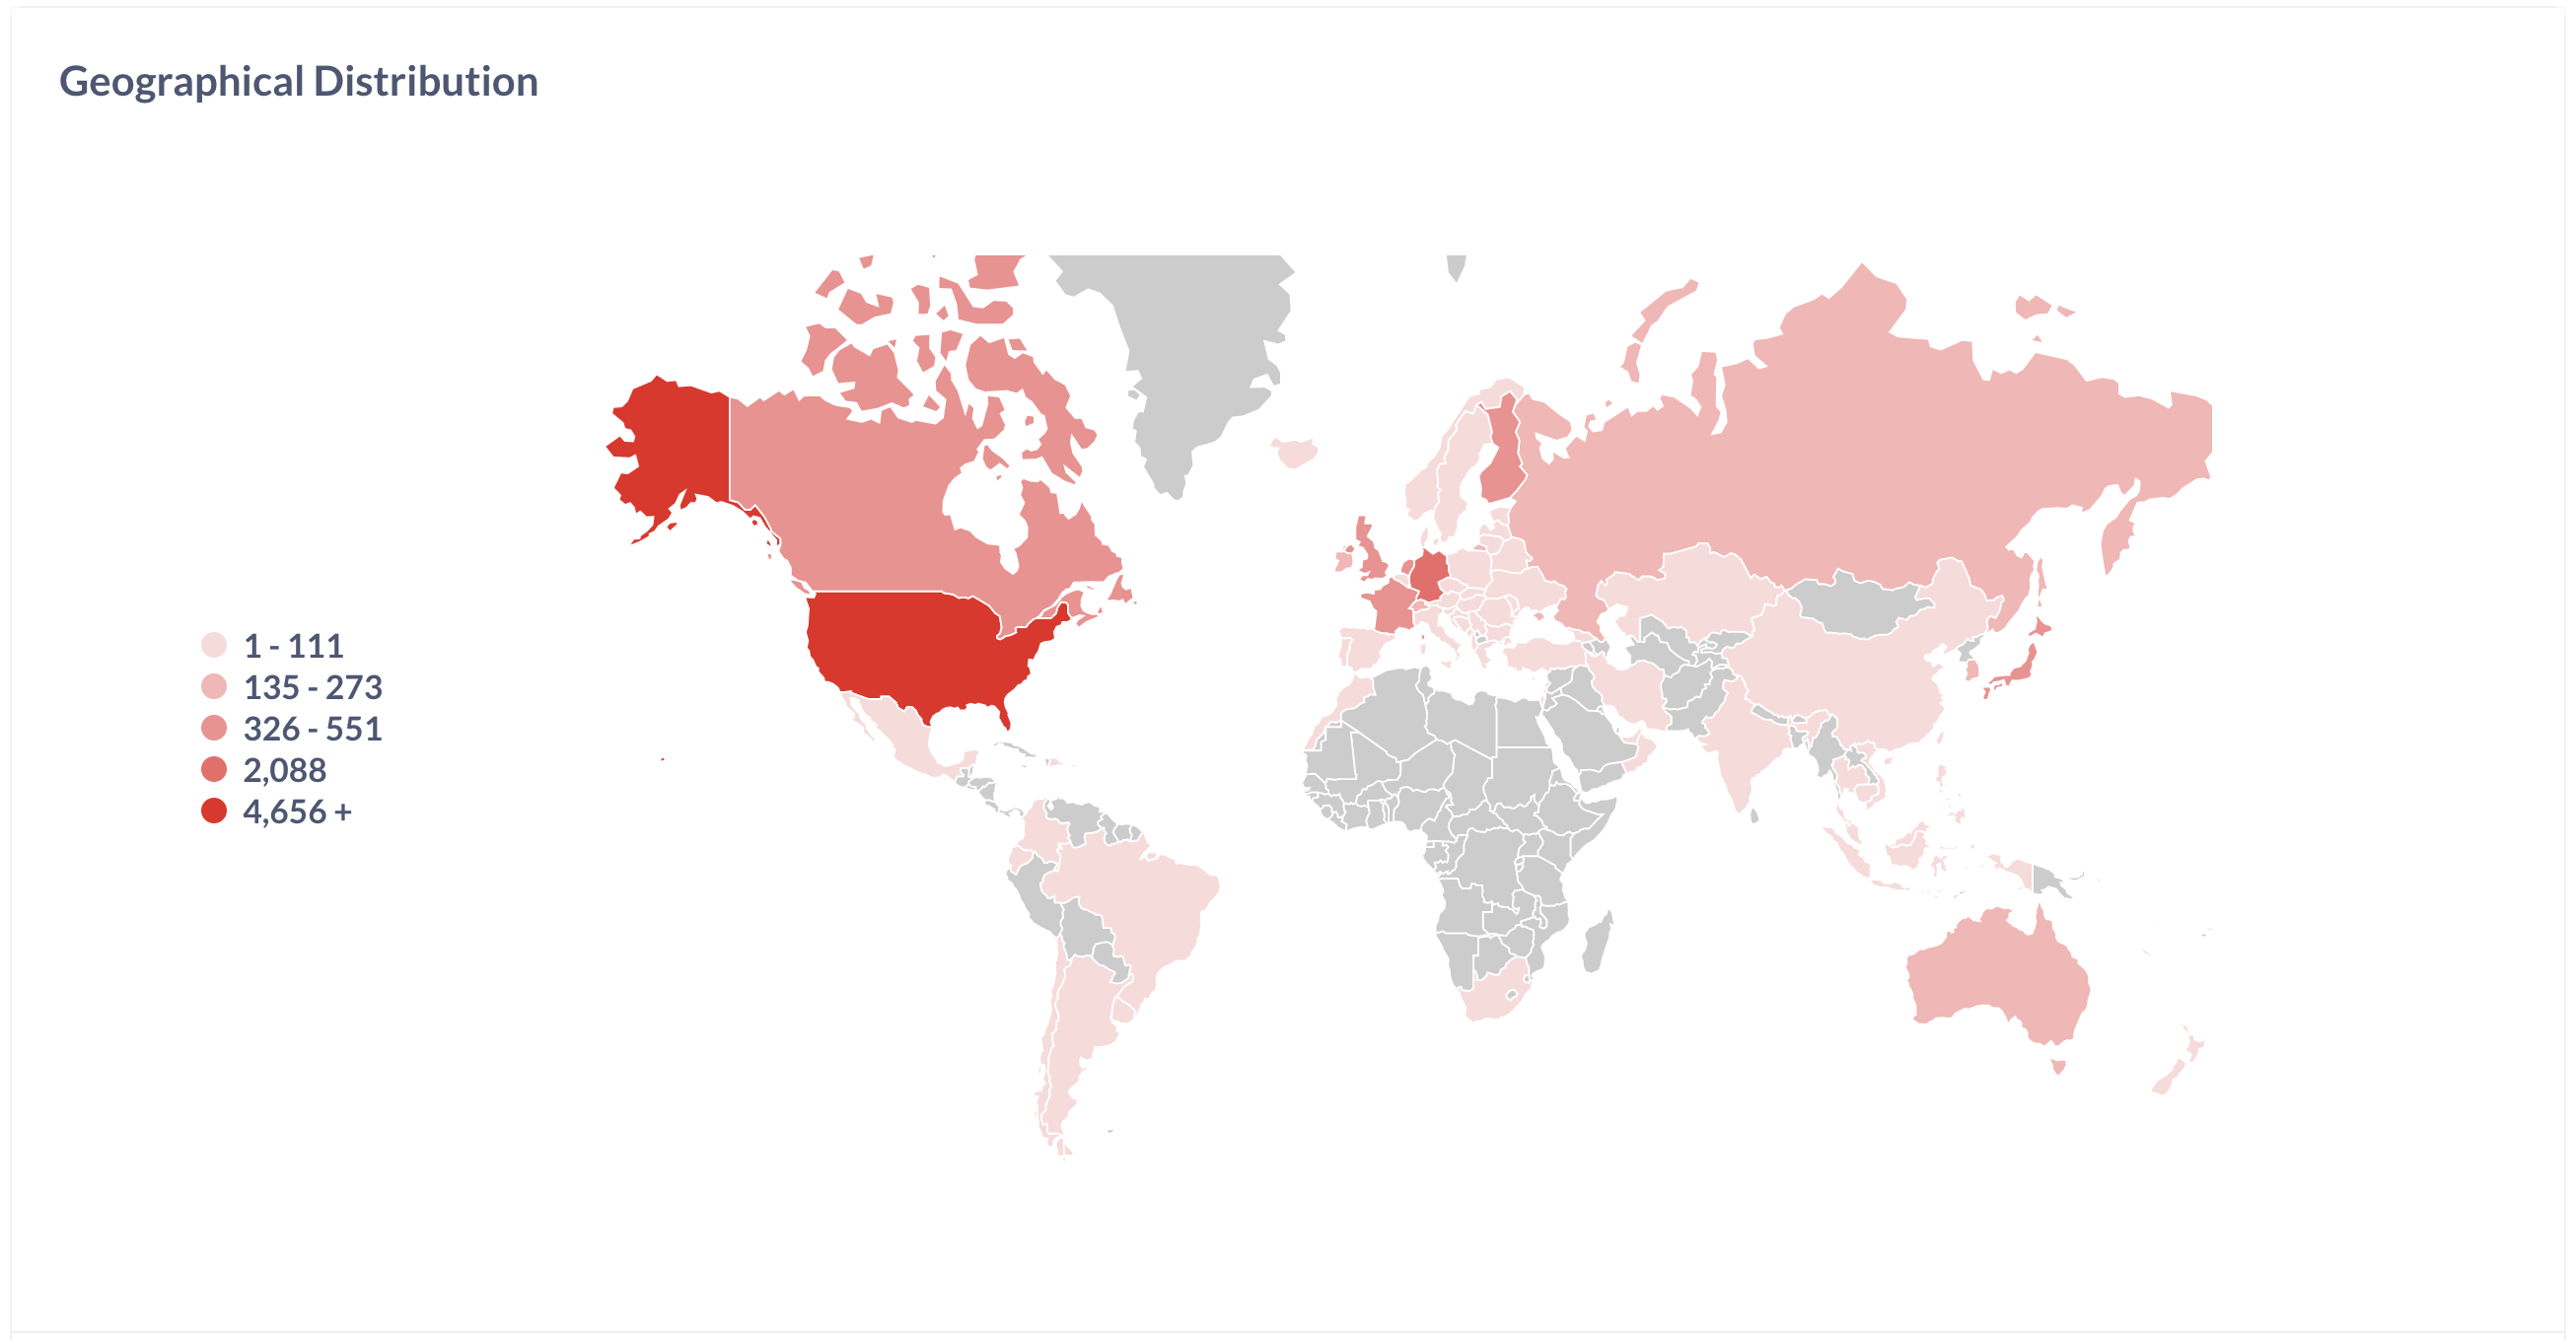
\includegraphics[width=0.48\linewidth]{images/geographical} \\
(a)\hspace{160pt}        (b)\\
\caption{Distribution of active beacon chain nodes round trip time (RTT) from Migalabs (a) and geographical distribution (b) (9 May 2023)}
\label{fig:rtt}
\end{center}
\end{figure}

\begin{figure}[htbp]
\begin{center}
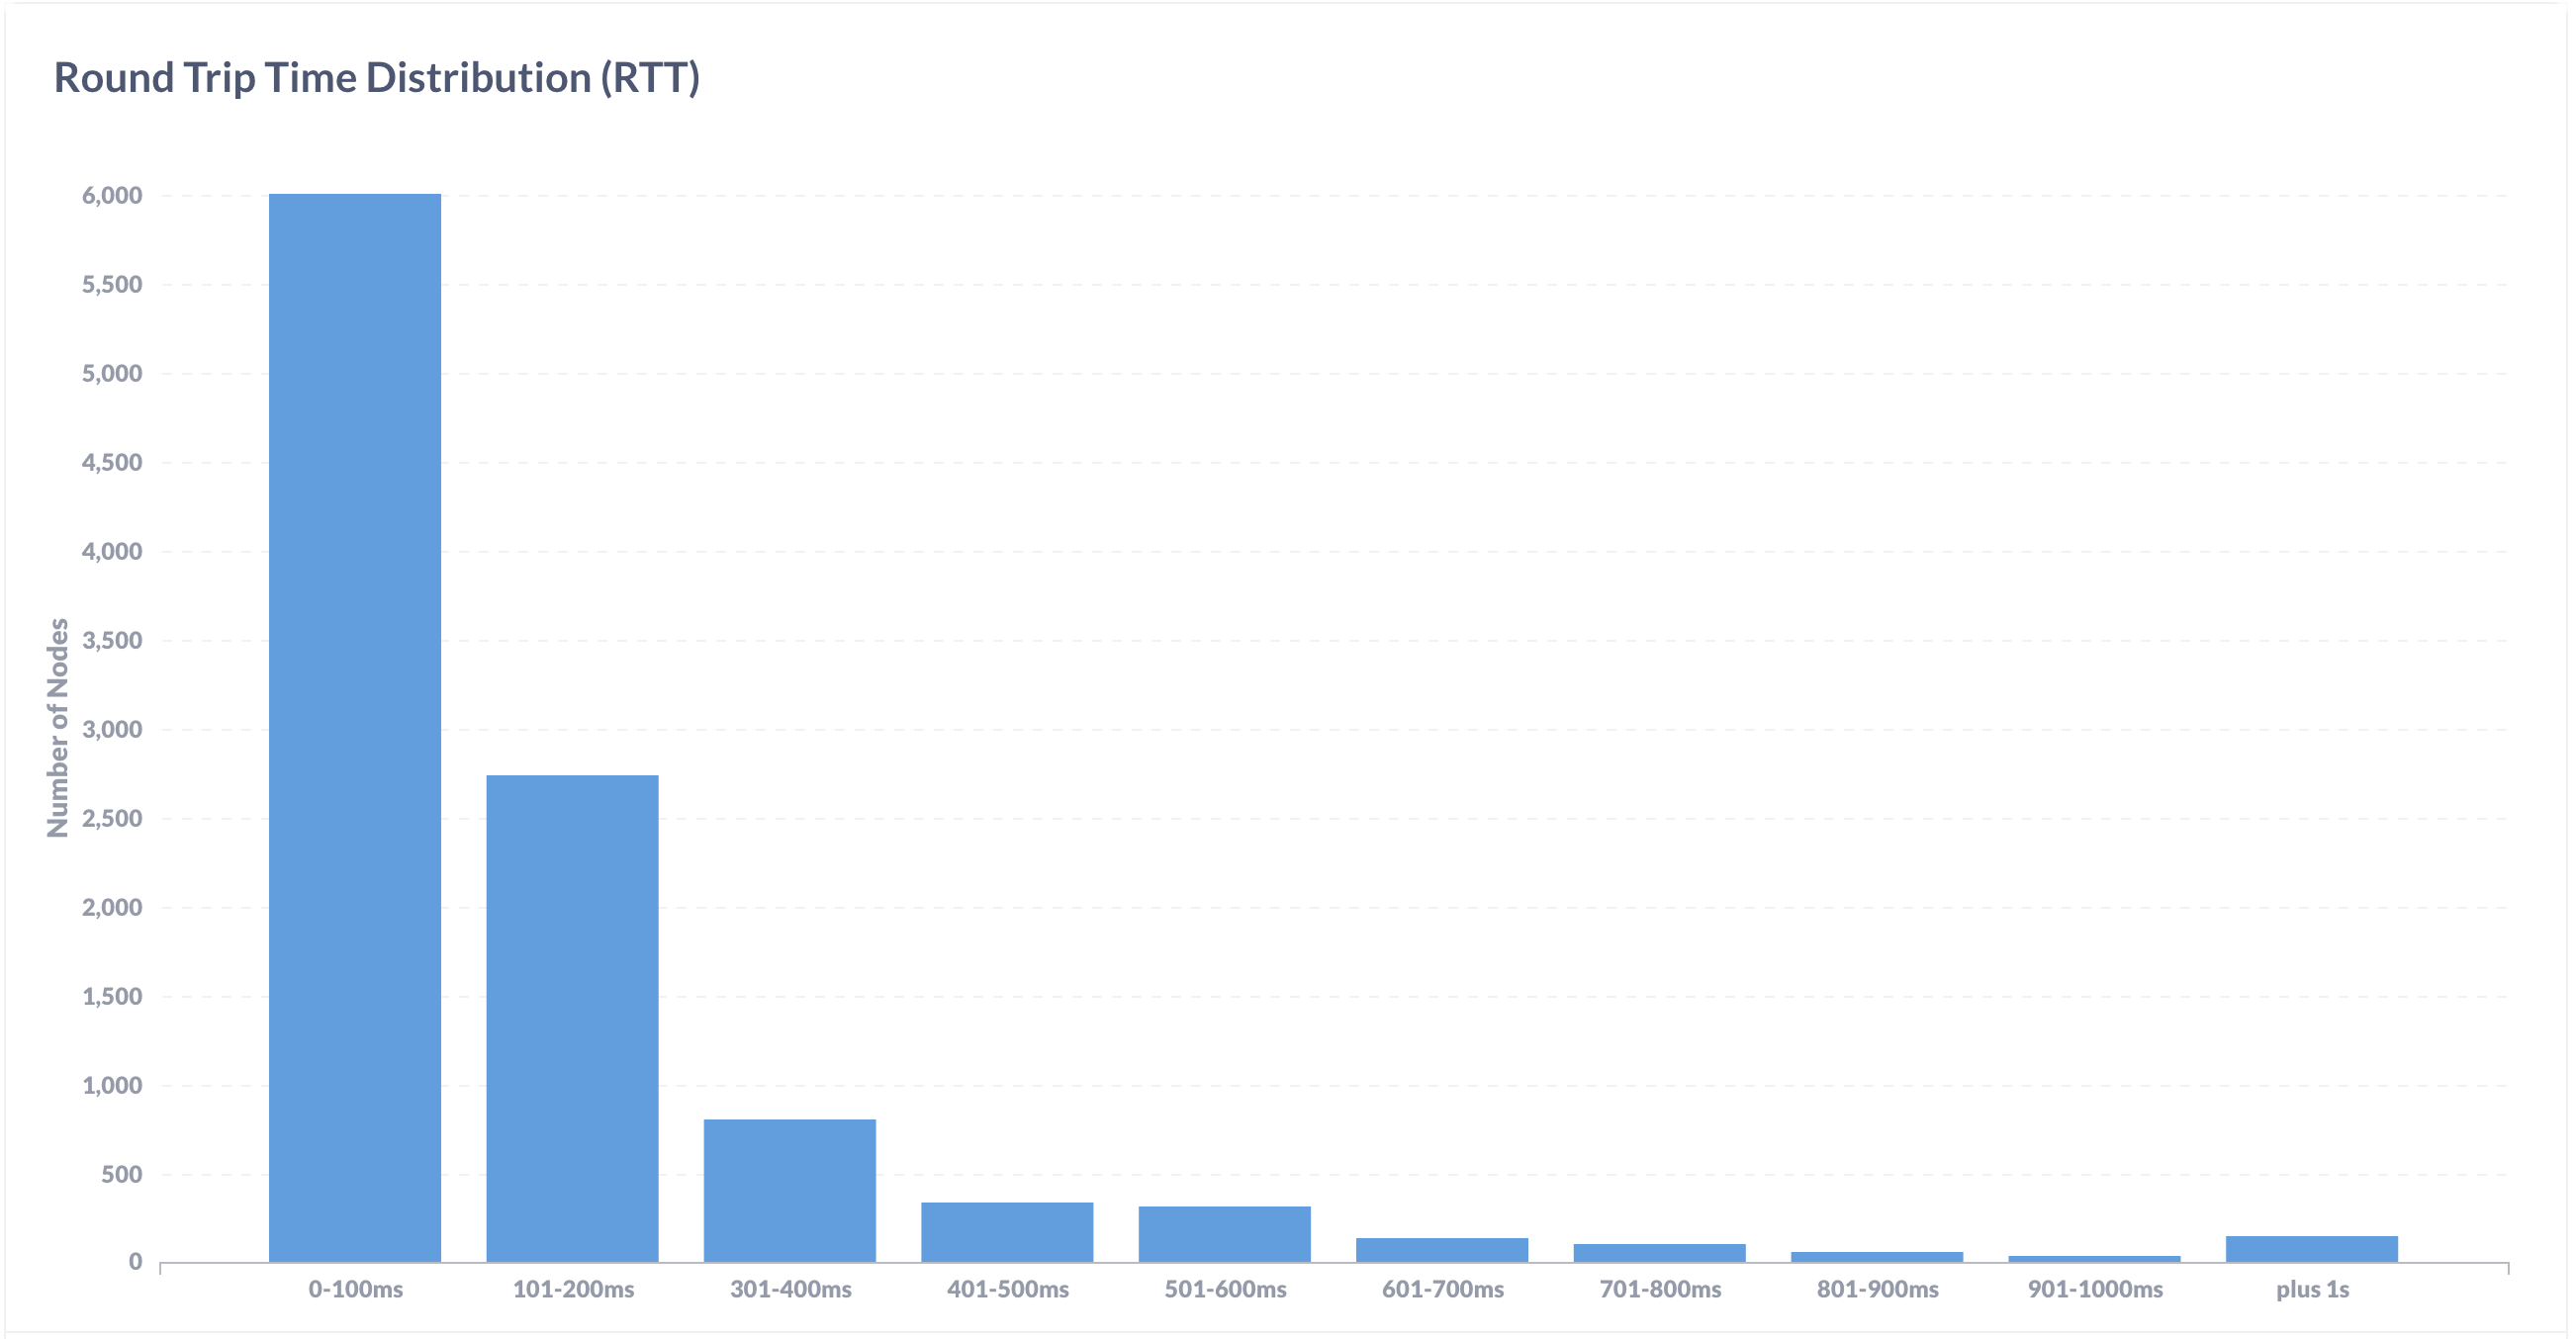
\includegraphics[width=0.48\linewidth]{images/rttdist}
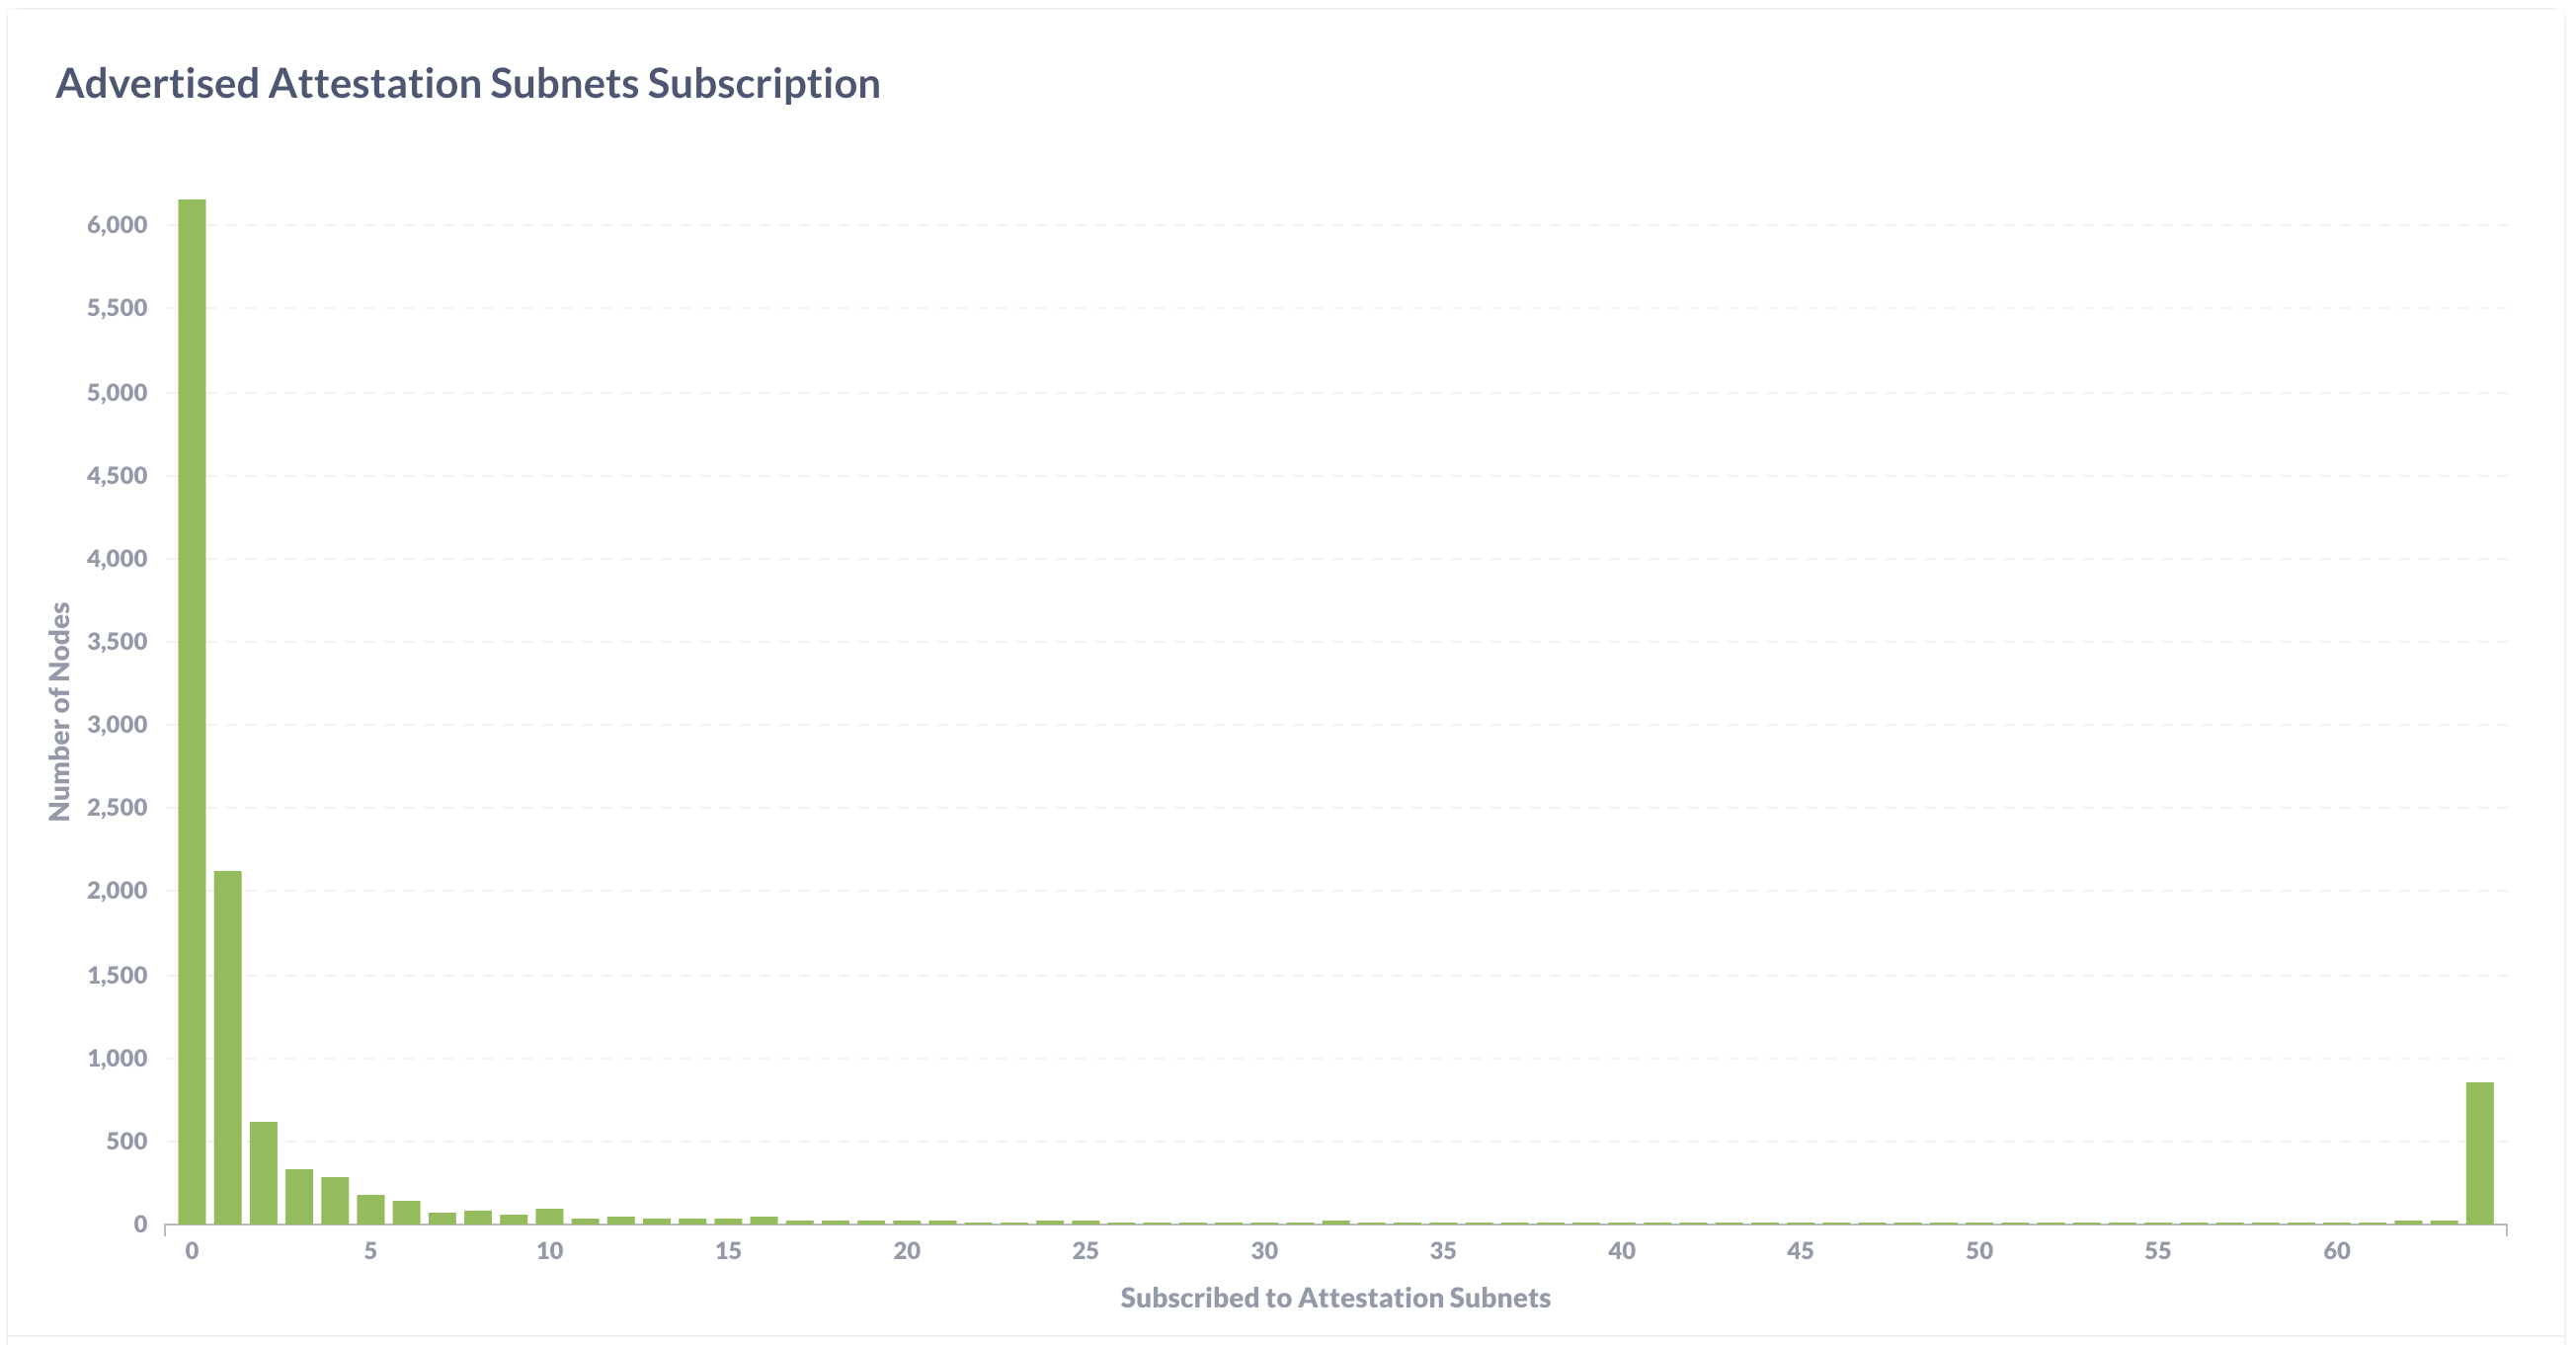
\includegraphics[width=0.48\linewidth]{images/aass} \\
(a)\hspace{160pt}        (b)\\
\caption{Distribution of active beacon chain nodes round trip time distribution (RTT) from Migalabs (a) and advertised attestation subnets subscription (b) (9 May 2023)}
\label{fig:aass}
\end{center}
\end{figure}

\begin{figure}[htbp]
\begin{center}
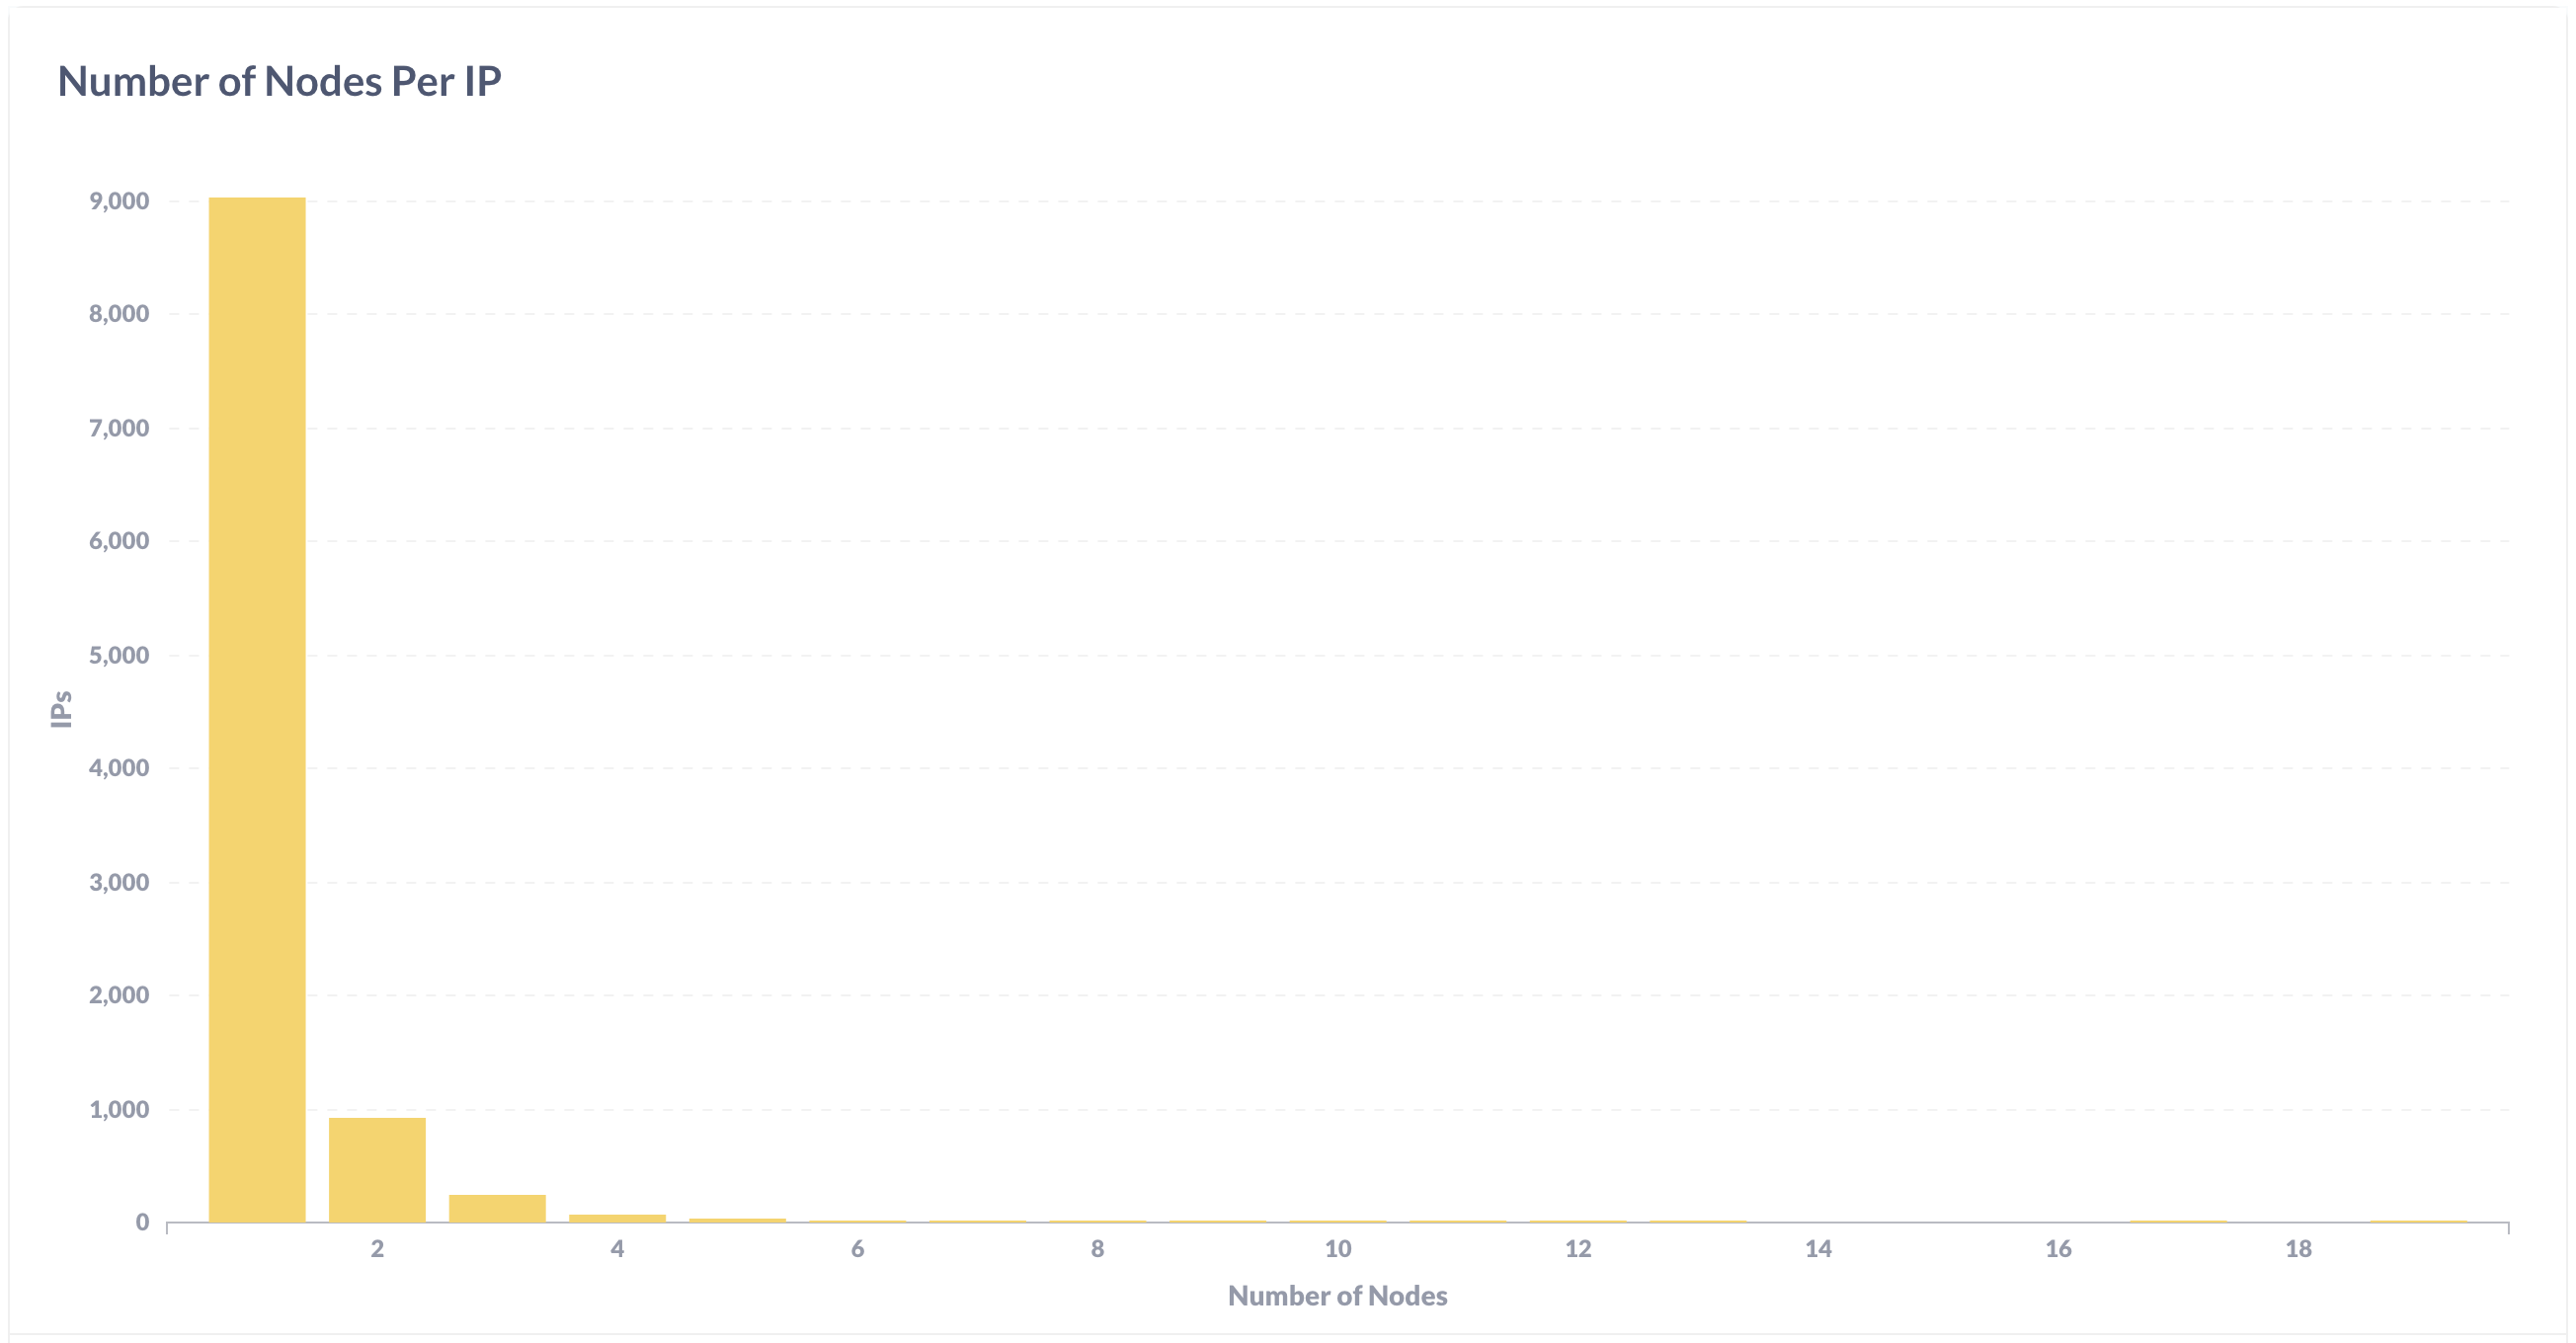
\includegraphics[width=0.48\linewidth]{images/ipdist}
\caption{Number of beacon nodes per IP from Migalabs }
\label{fig:ipdist}
\end{center}
\end{figure}
\clearpage
% --------------------------------------
\subsubsection*{Ultrasound money}
% --------------------------------------

\begin{figure}[htbp]
\begin{center}
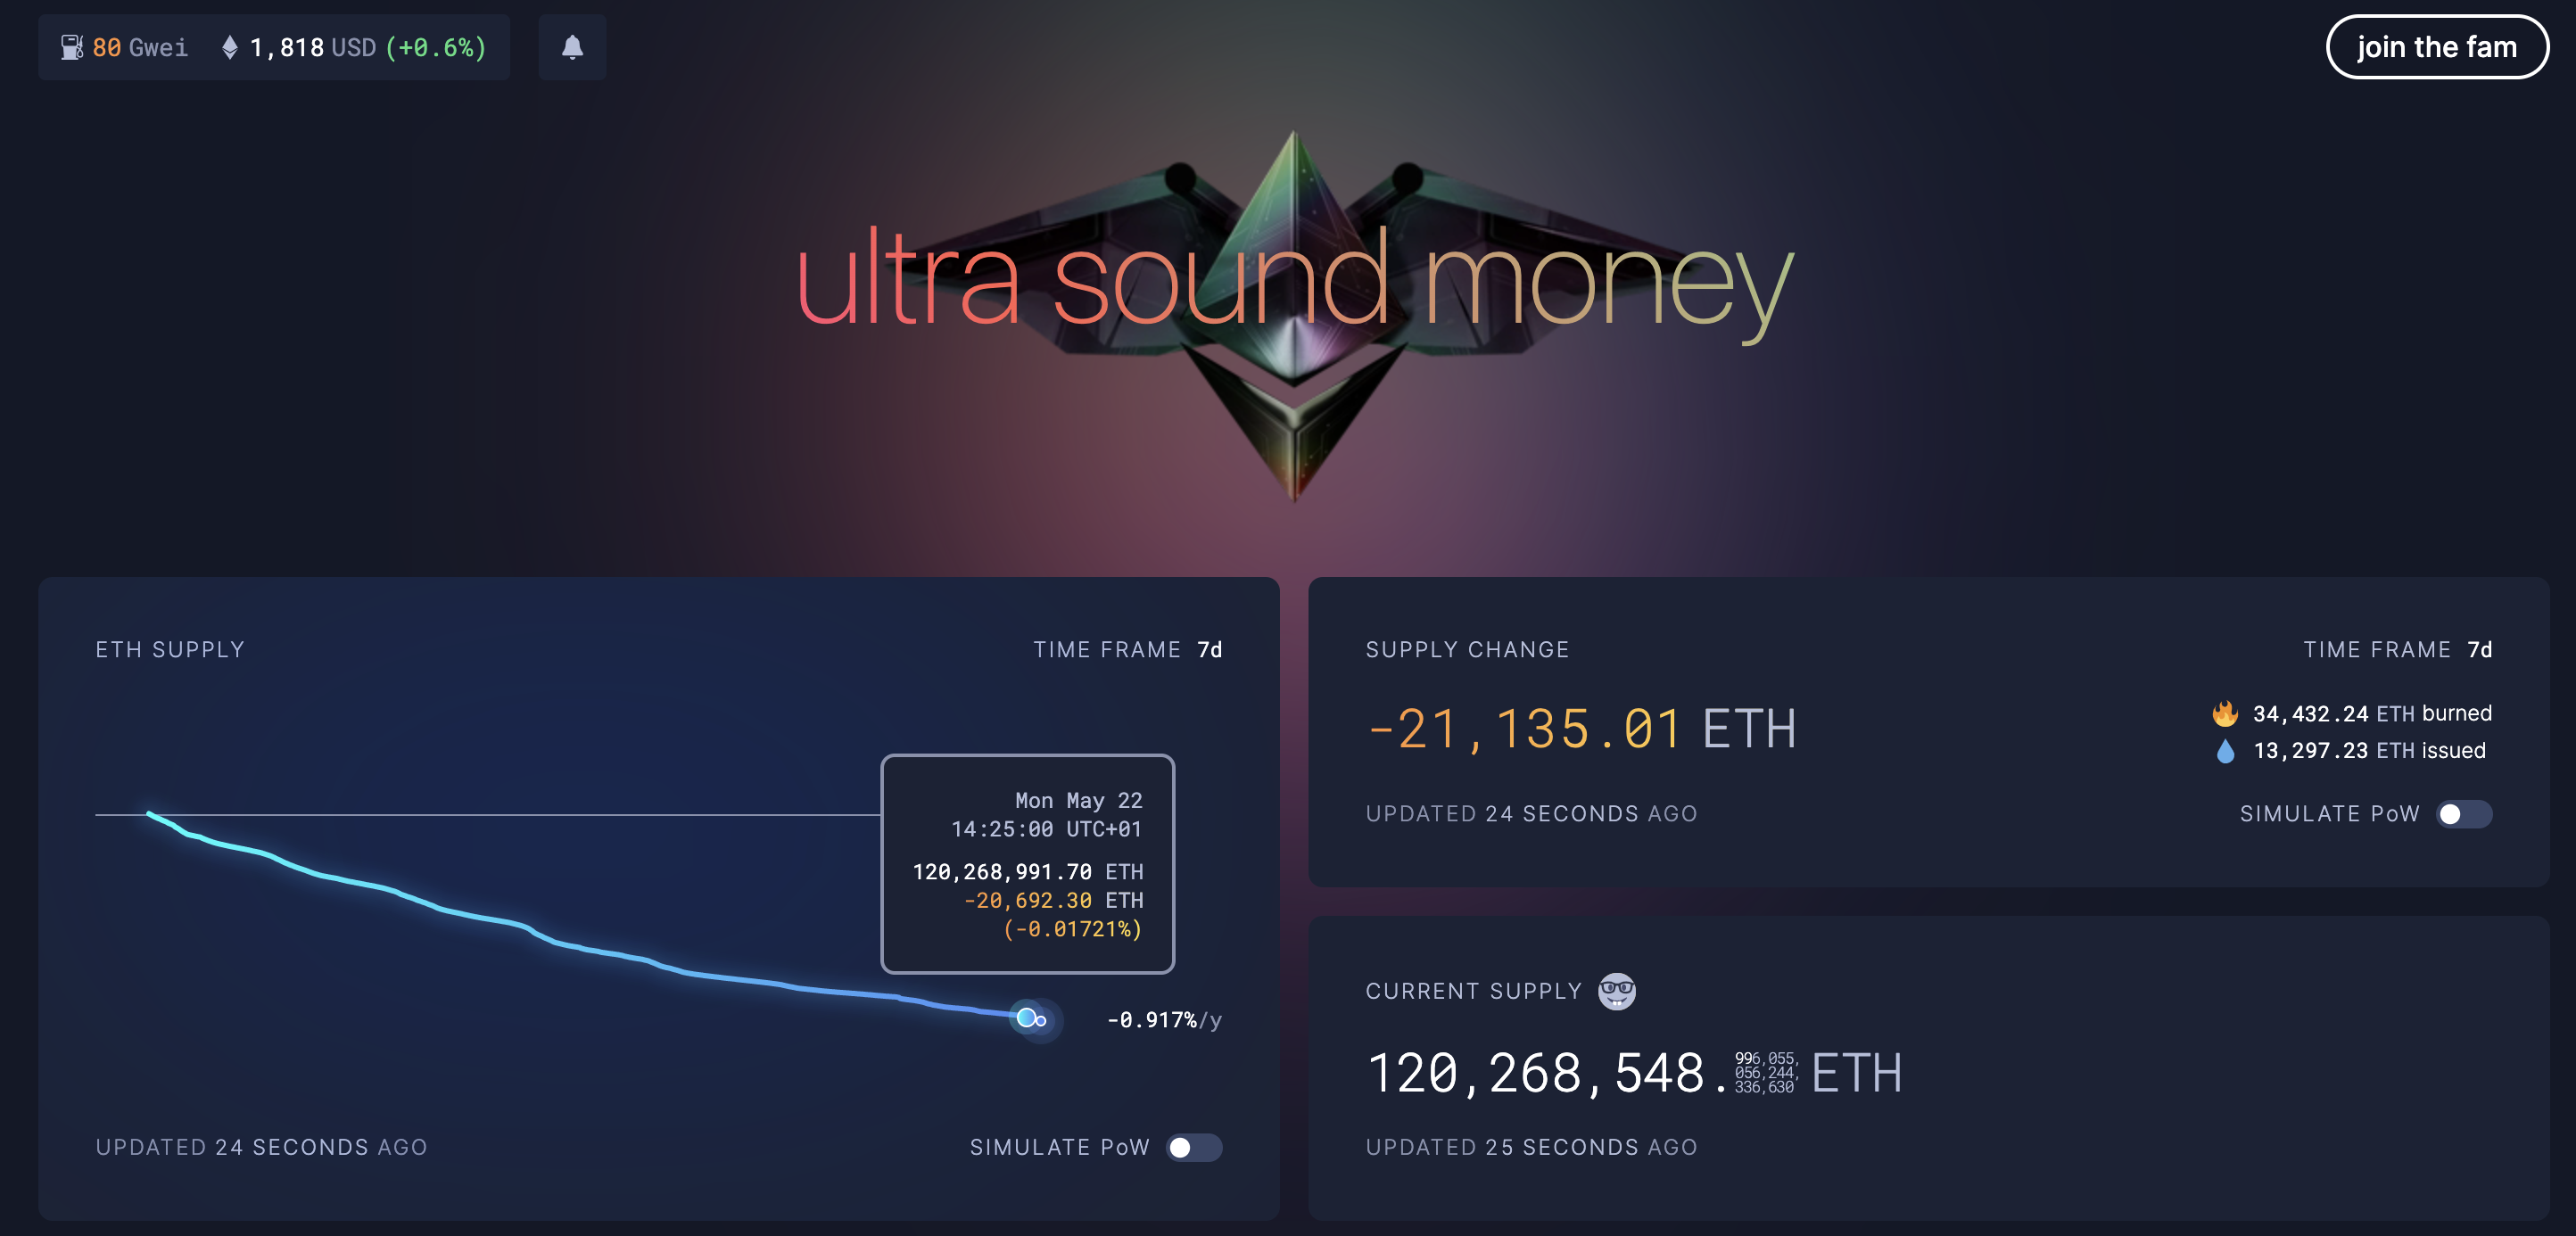
\includegraphics[width=0.9\linewidth]{images/ethsupply}
\caption{ETH supply over time, current supply and change, 22 May 2023}
\label{fig:ethsupply}
\end{center}
\end{figure}

\begin{figure}[htbp]
\begin{center}
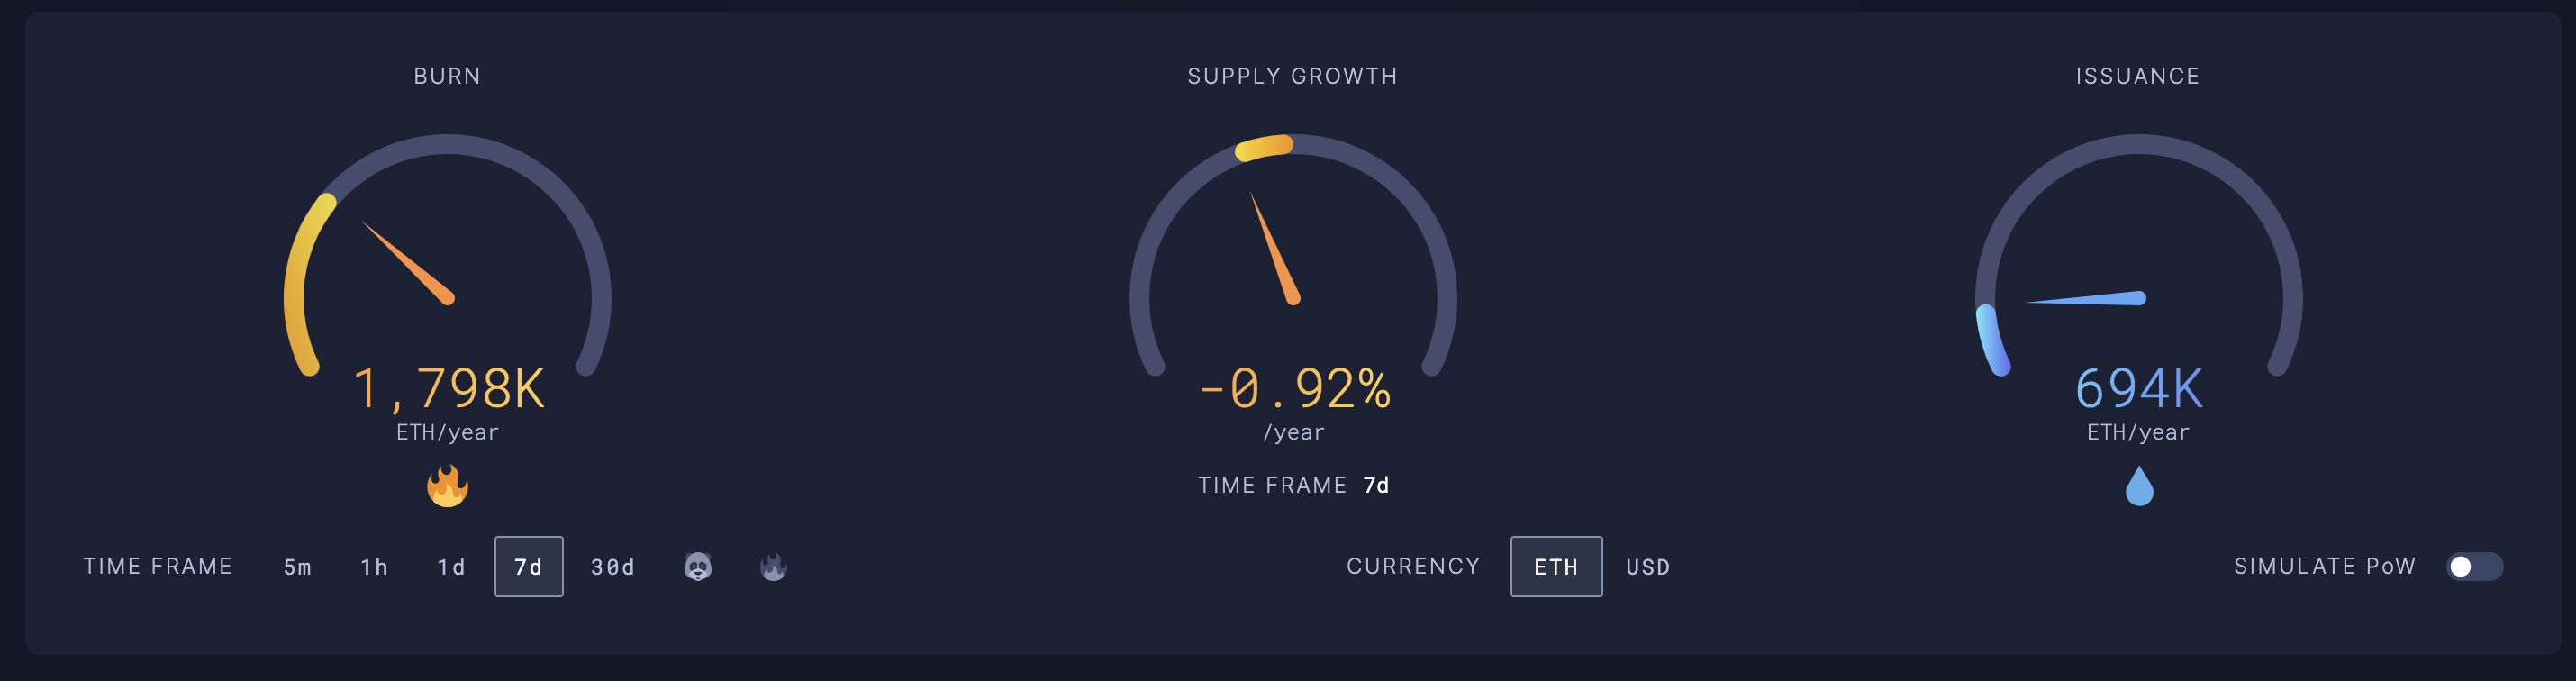
\includegraphics[width=0.9\linewidth]{images/burn}
\caption{Burn, supply growth, and issuance, 22 May 2023}
\label{fig:burn}
\end{center}
\end{figure}

\begin{figure}[htbp]
\begin{center}
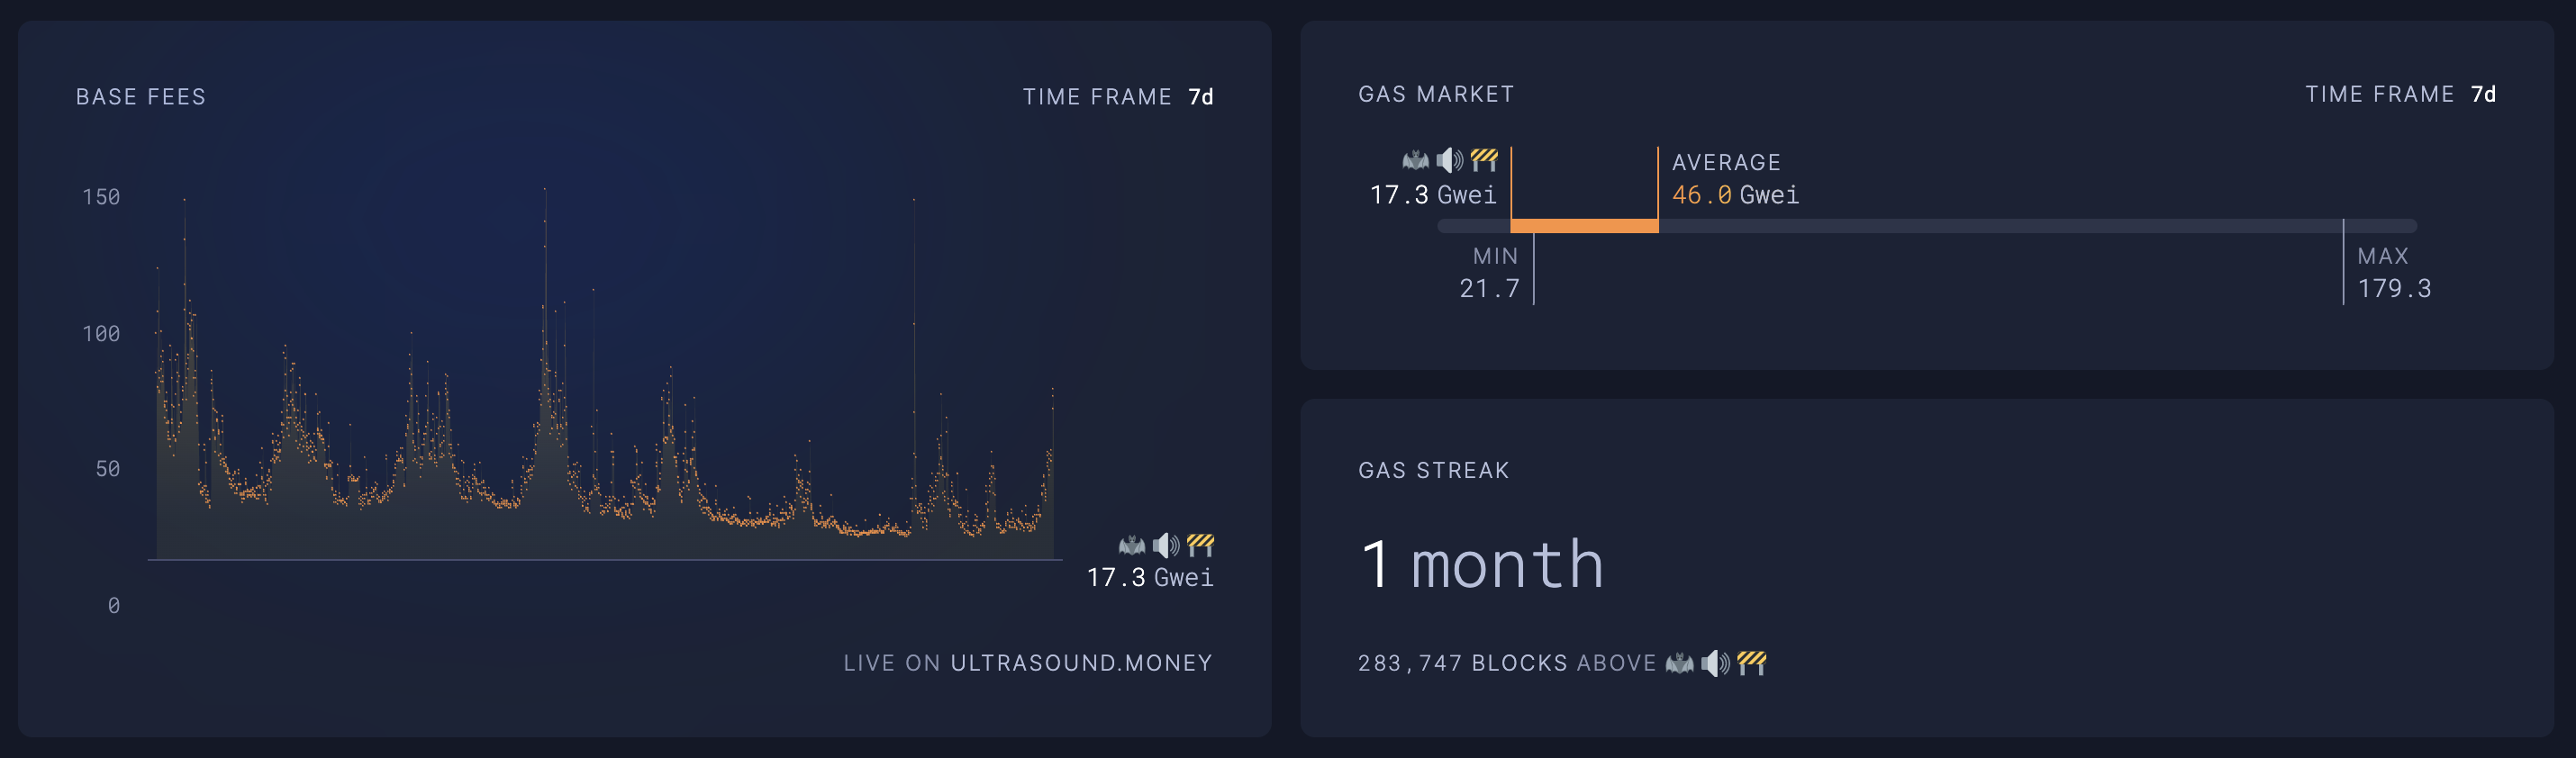
\includegraphics[width=0.9\linewidth]{images/gasmarket}
\caption{Gas market, 22 May 2023}
\label{fig:gas}
\end{center}
\end{figure}

\begin{figure}[htbp]
\begin{center}
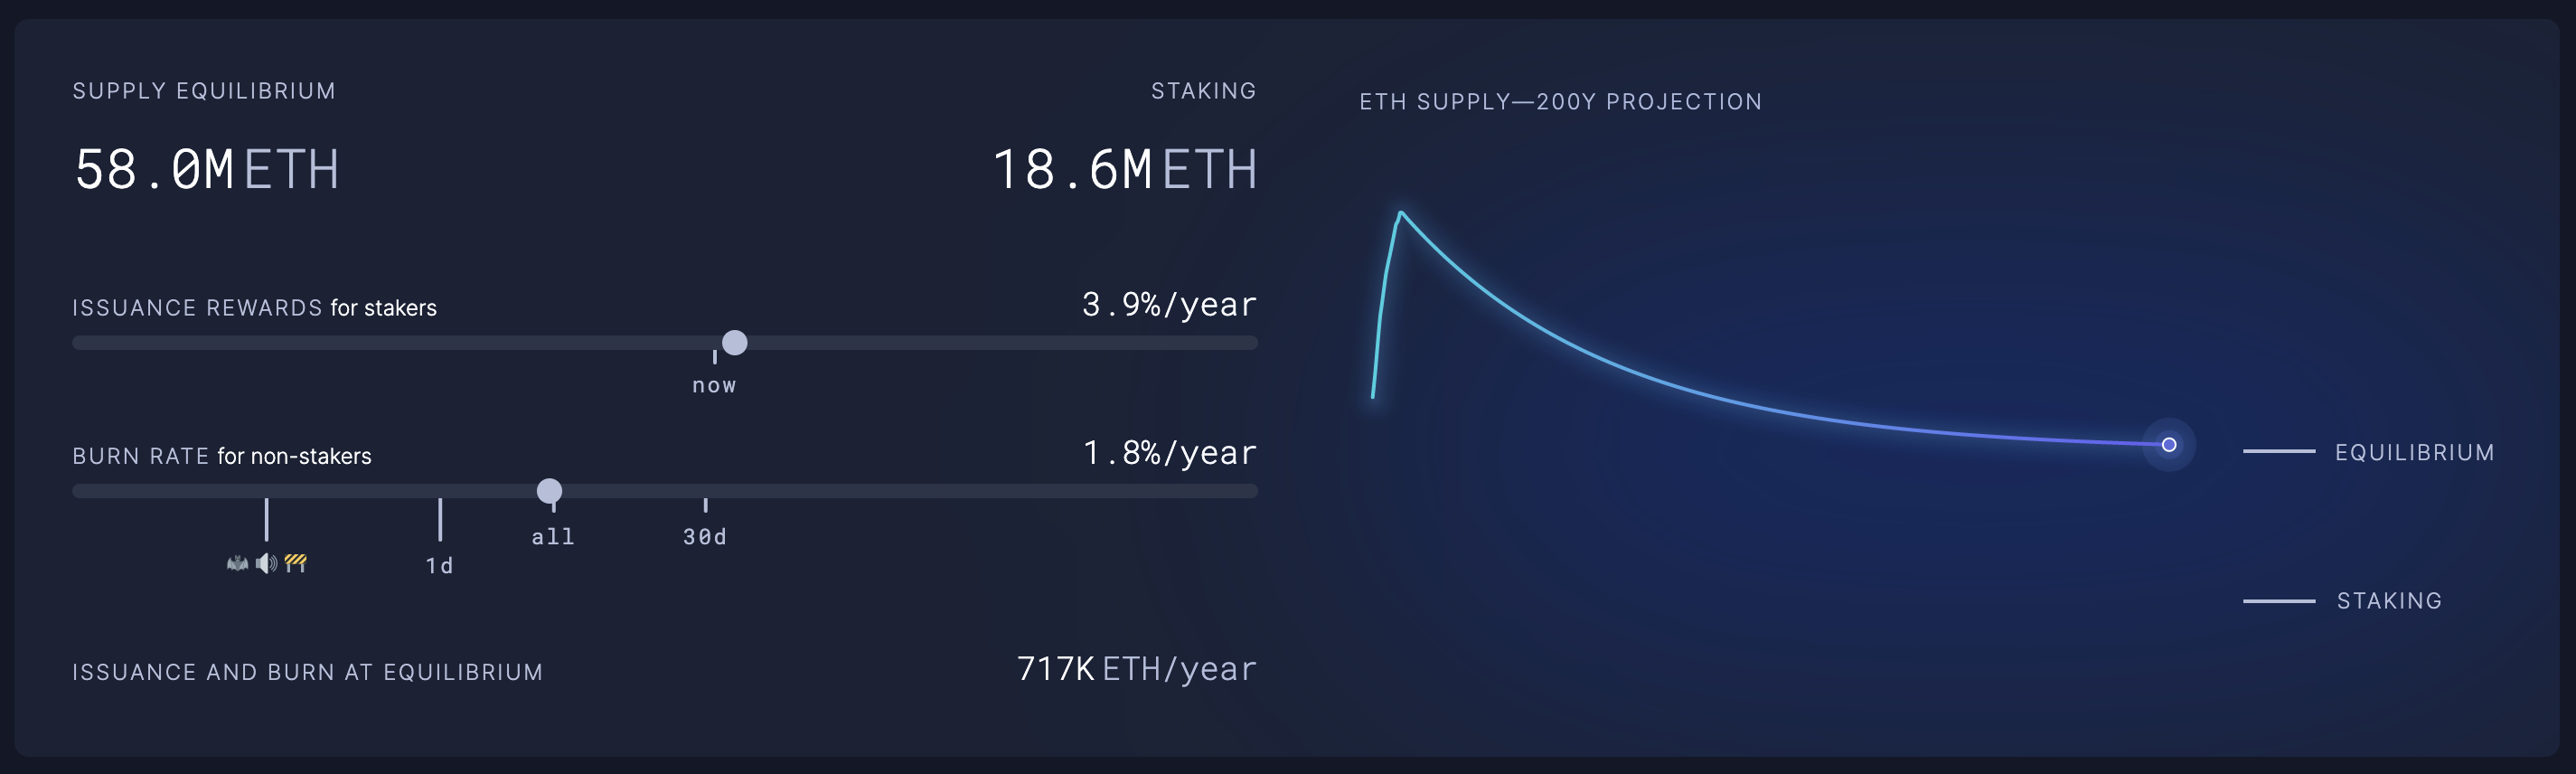
\includegraphics[width=0.9\linewidth]{images/projection}
\caption{Interactive ETH supply projections - sliders provided for issuance rewards and burn rate , 22 May 2023}
\label{fig:projection}
\end{center}
\end{figure}

\begin{figure}[htbp]
\begin{center}
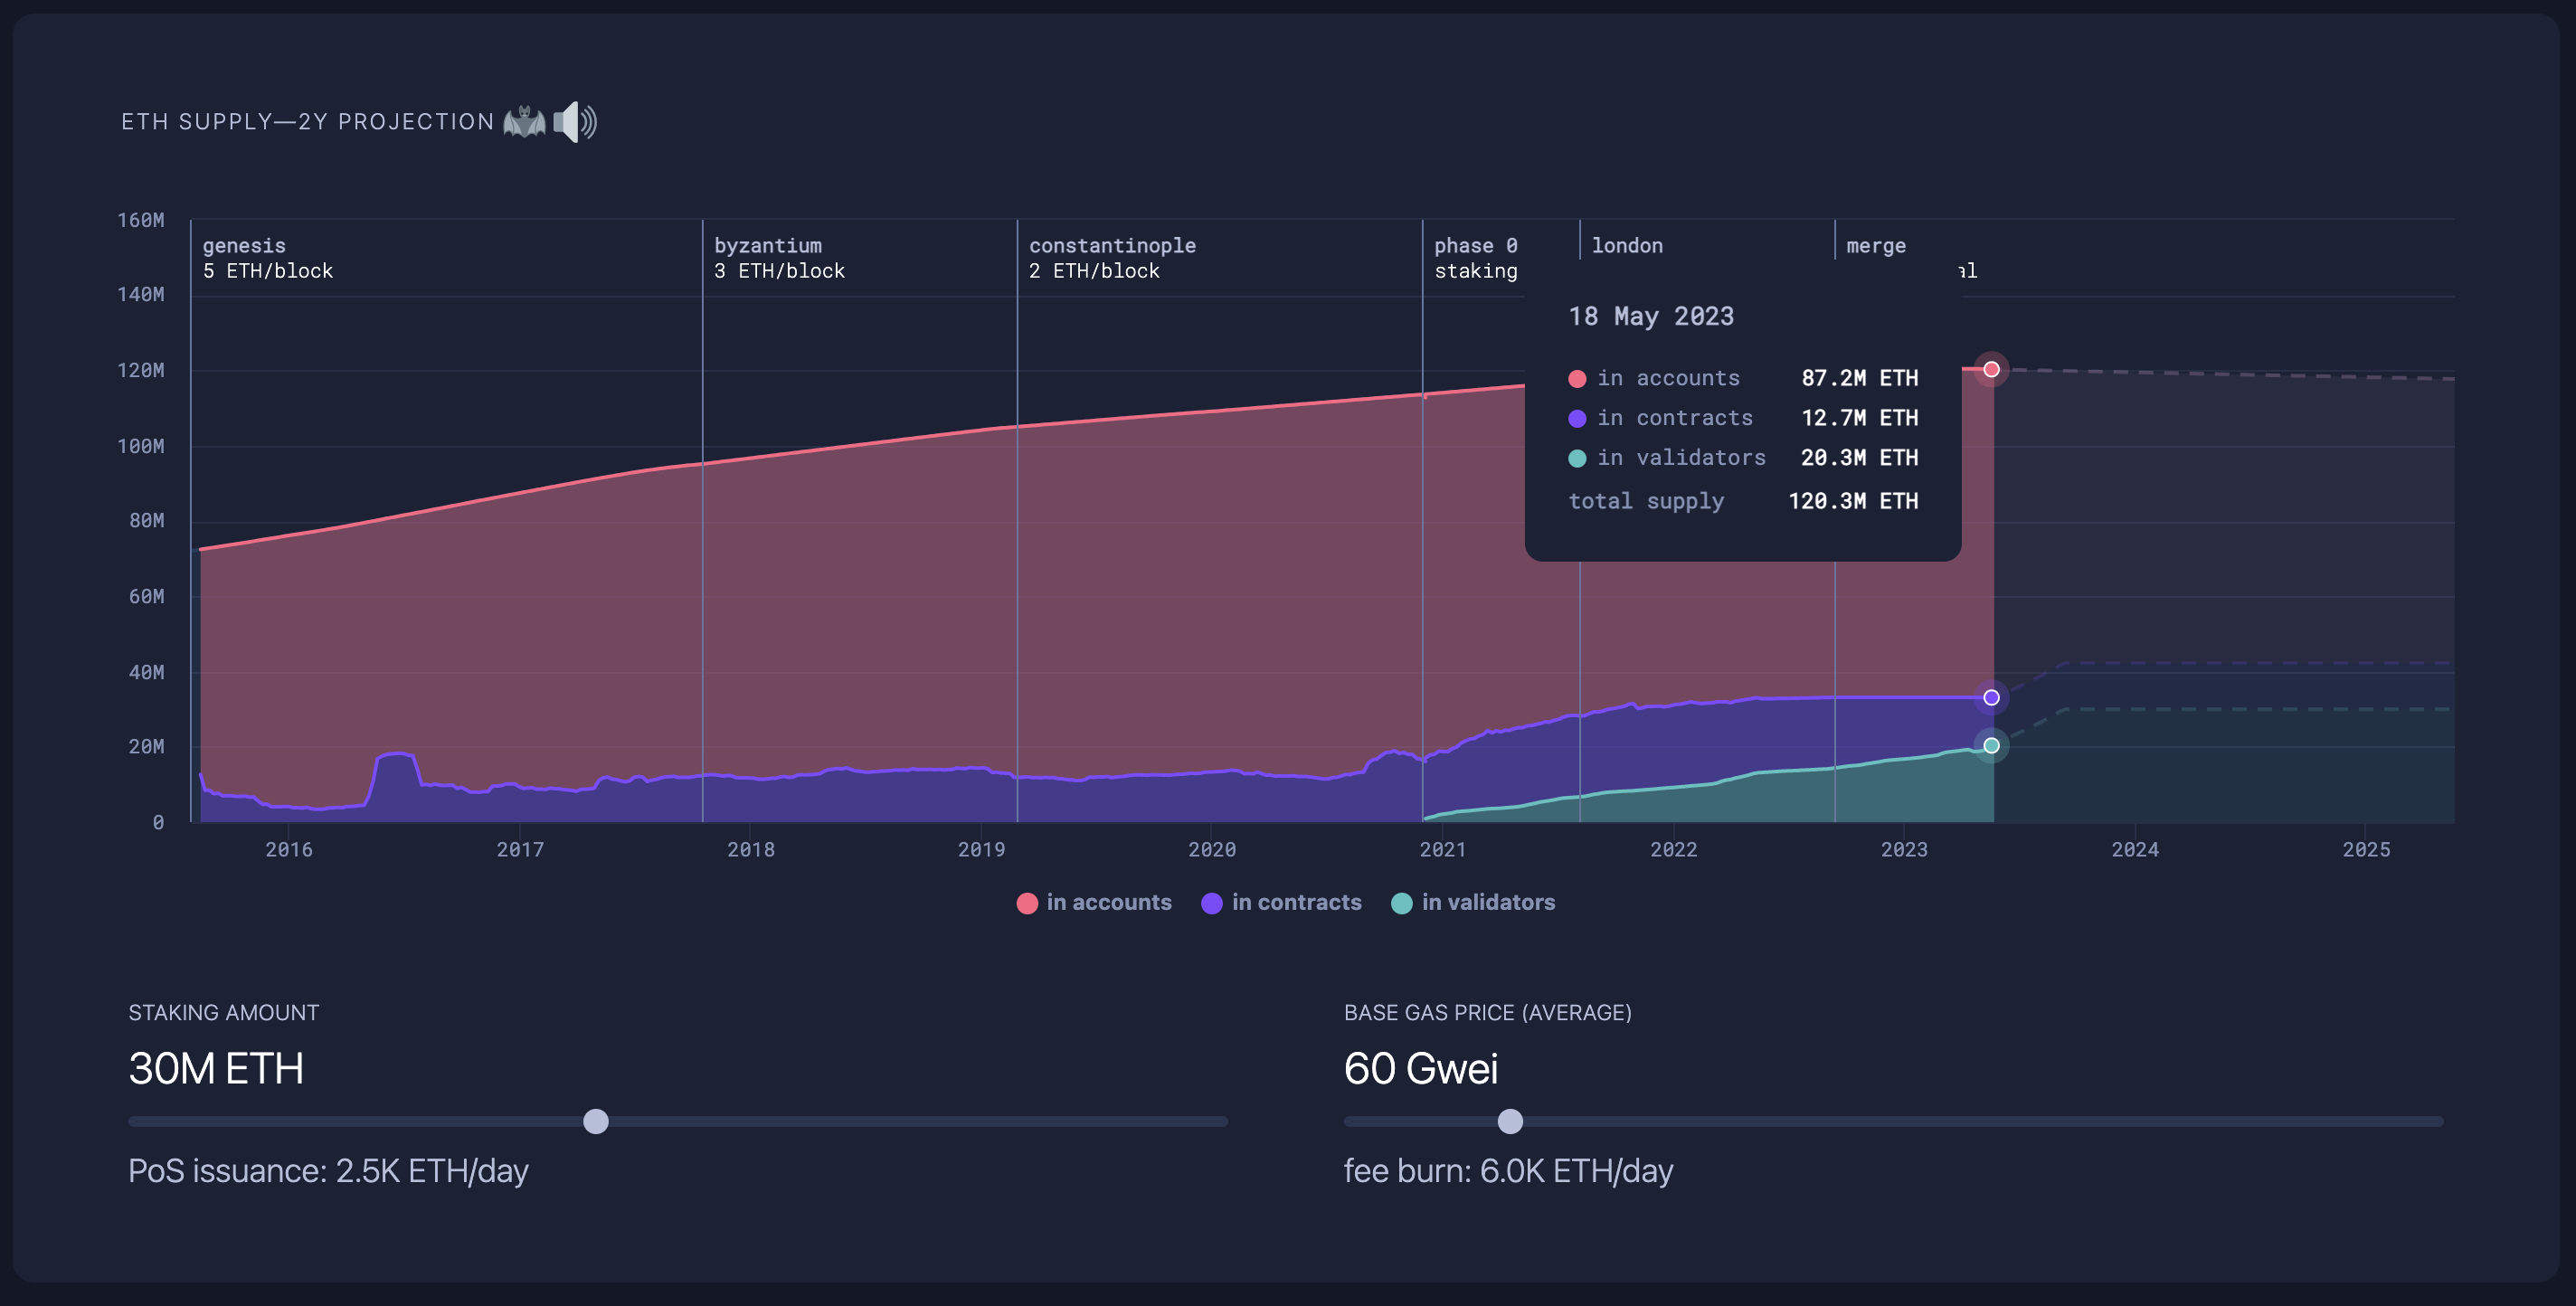
\includegraphics[width=0.9\linewidth]{images/2yprojection}
\caption{2YETH supply projection, 22 May 2023}
\label{fig:2yprojection}
\end{center}
\end{figure}

\begin{figure}[htbp]
\begin{center}
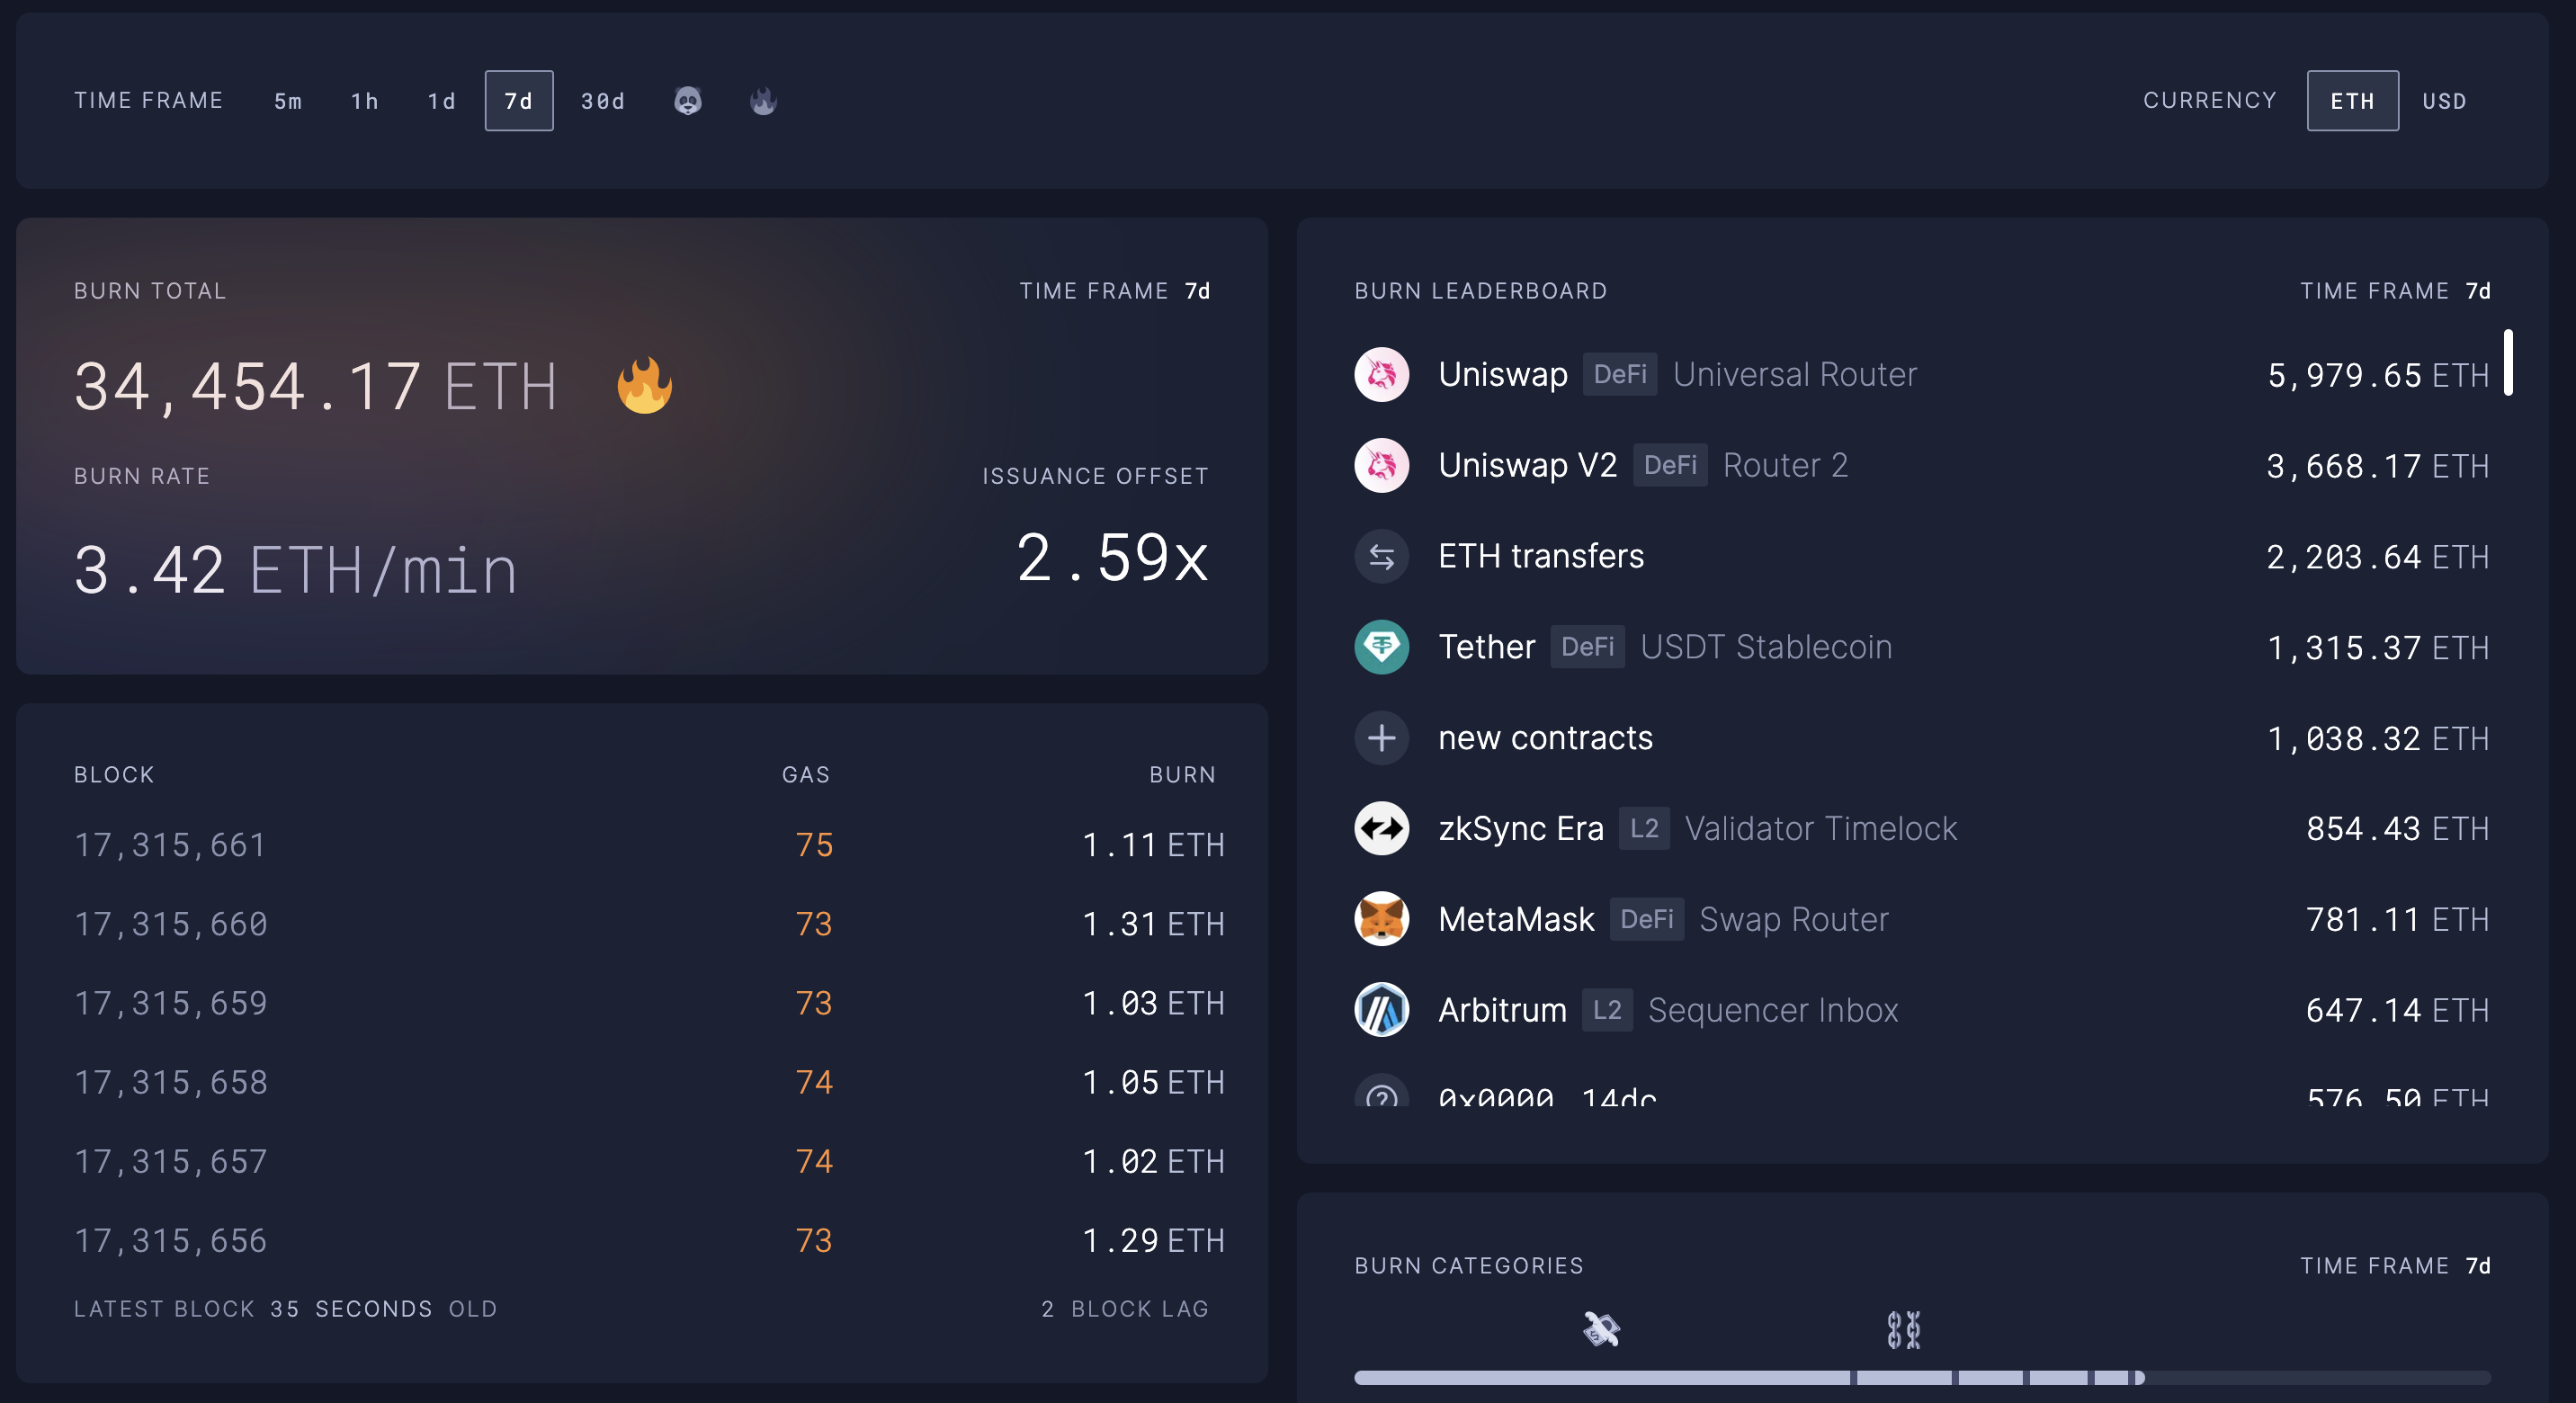
\includegraphics[width=0.9\linewidth]{images/totalburn}
\caption{Total burn and rate for selected time interval; latest block gas and burn leaderboard, 22 May 2023}
\label{fig:totalburn}
\end{center}
\end{figure}

\begin{figure}[htbp]
\begin{center}
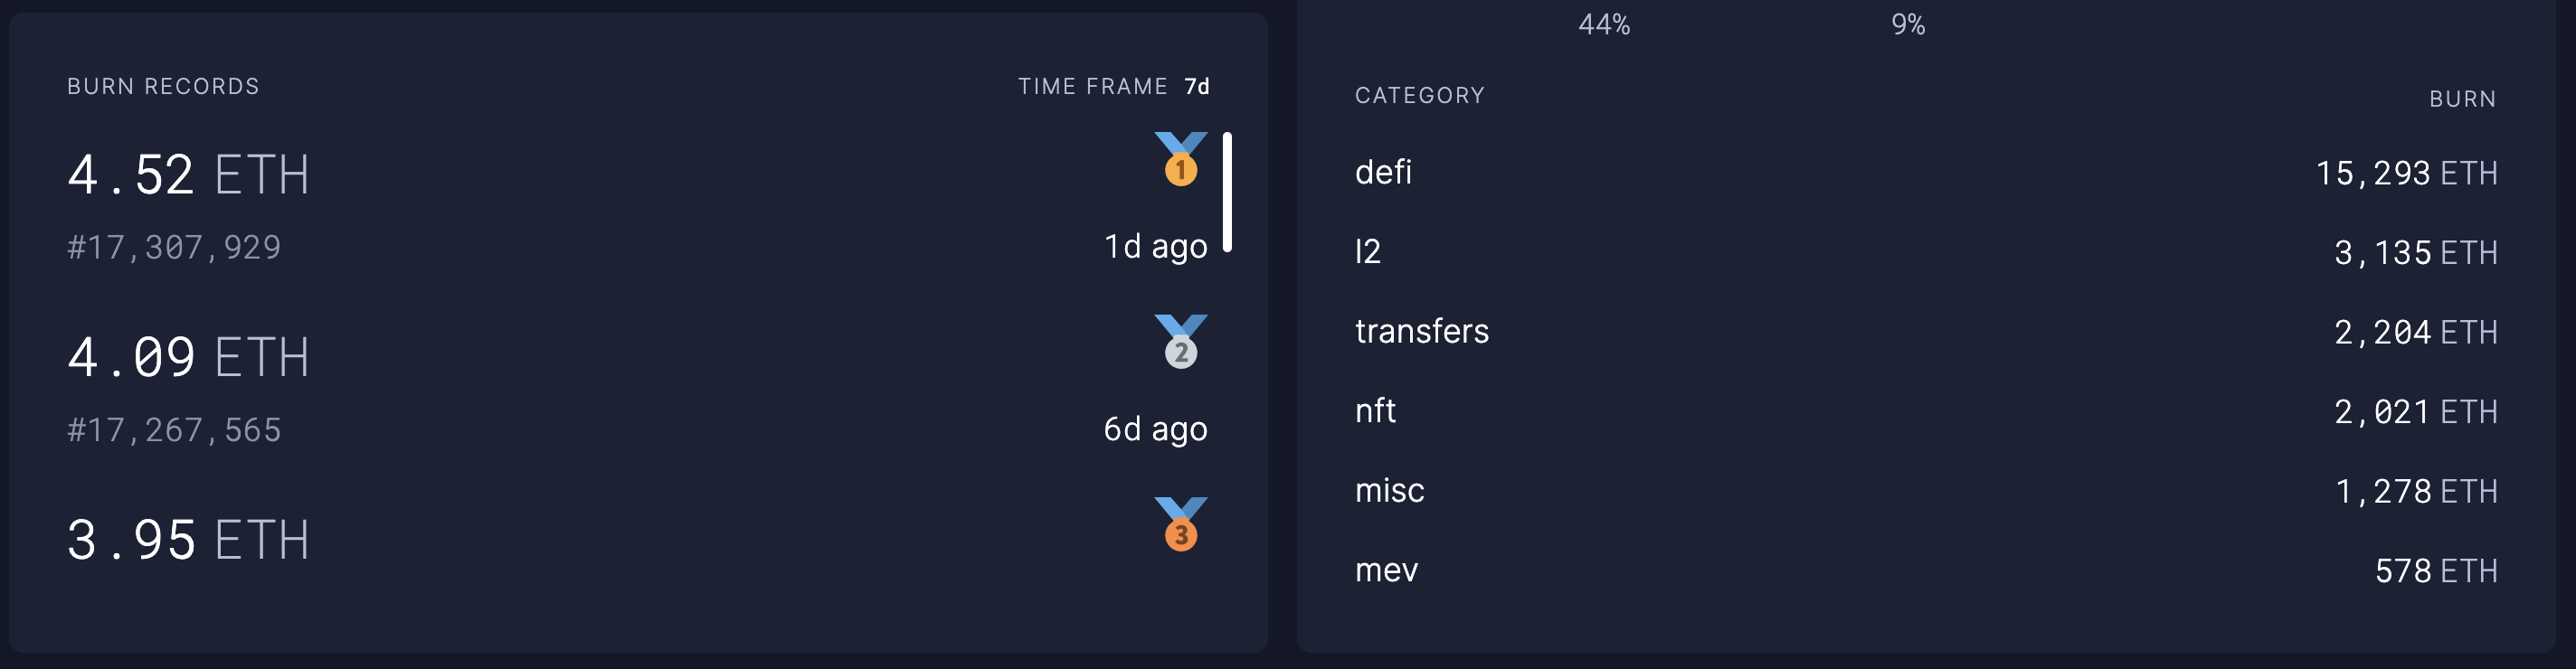
\includegraphics[width=0.9\linewidth]{images/records}
\caption{Burn records (top 3) and top 5 categories for most ETH burnt, 22 May 2023}
\label{fig:records}
\end{center}
\end{figure}

\begin{figure}[htbp]
\begin{center}
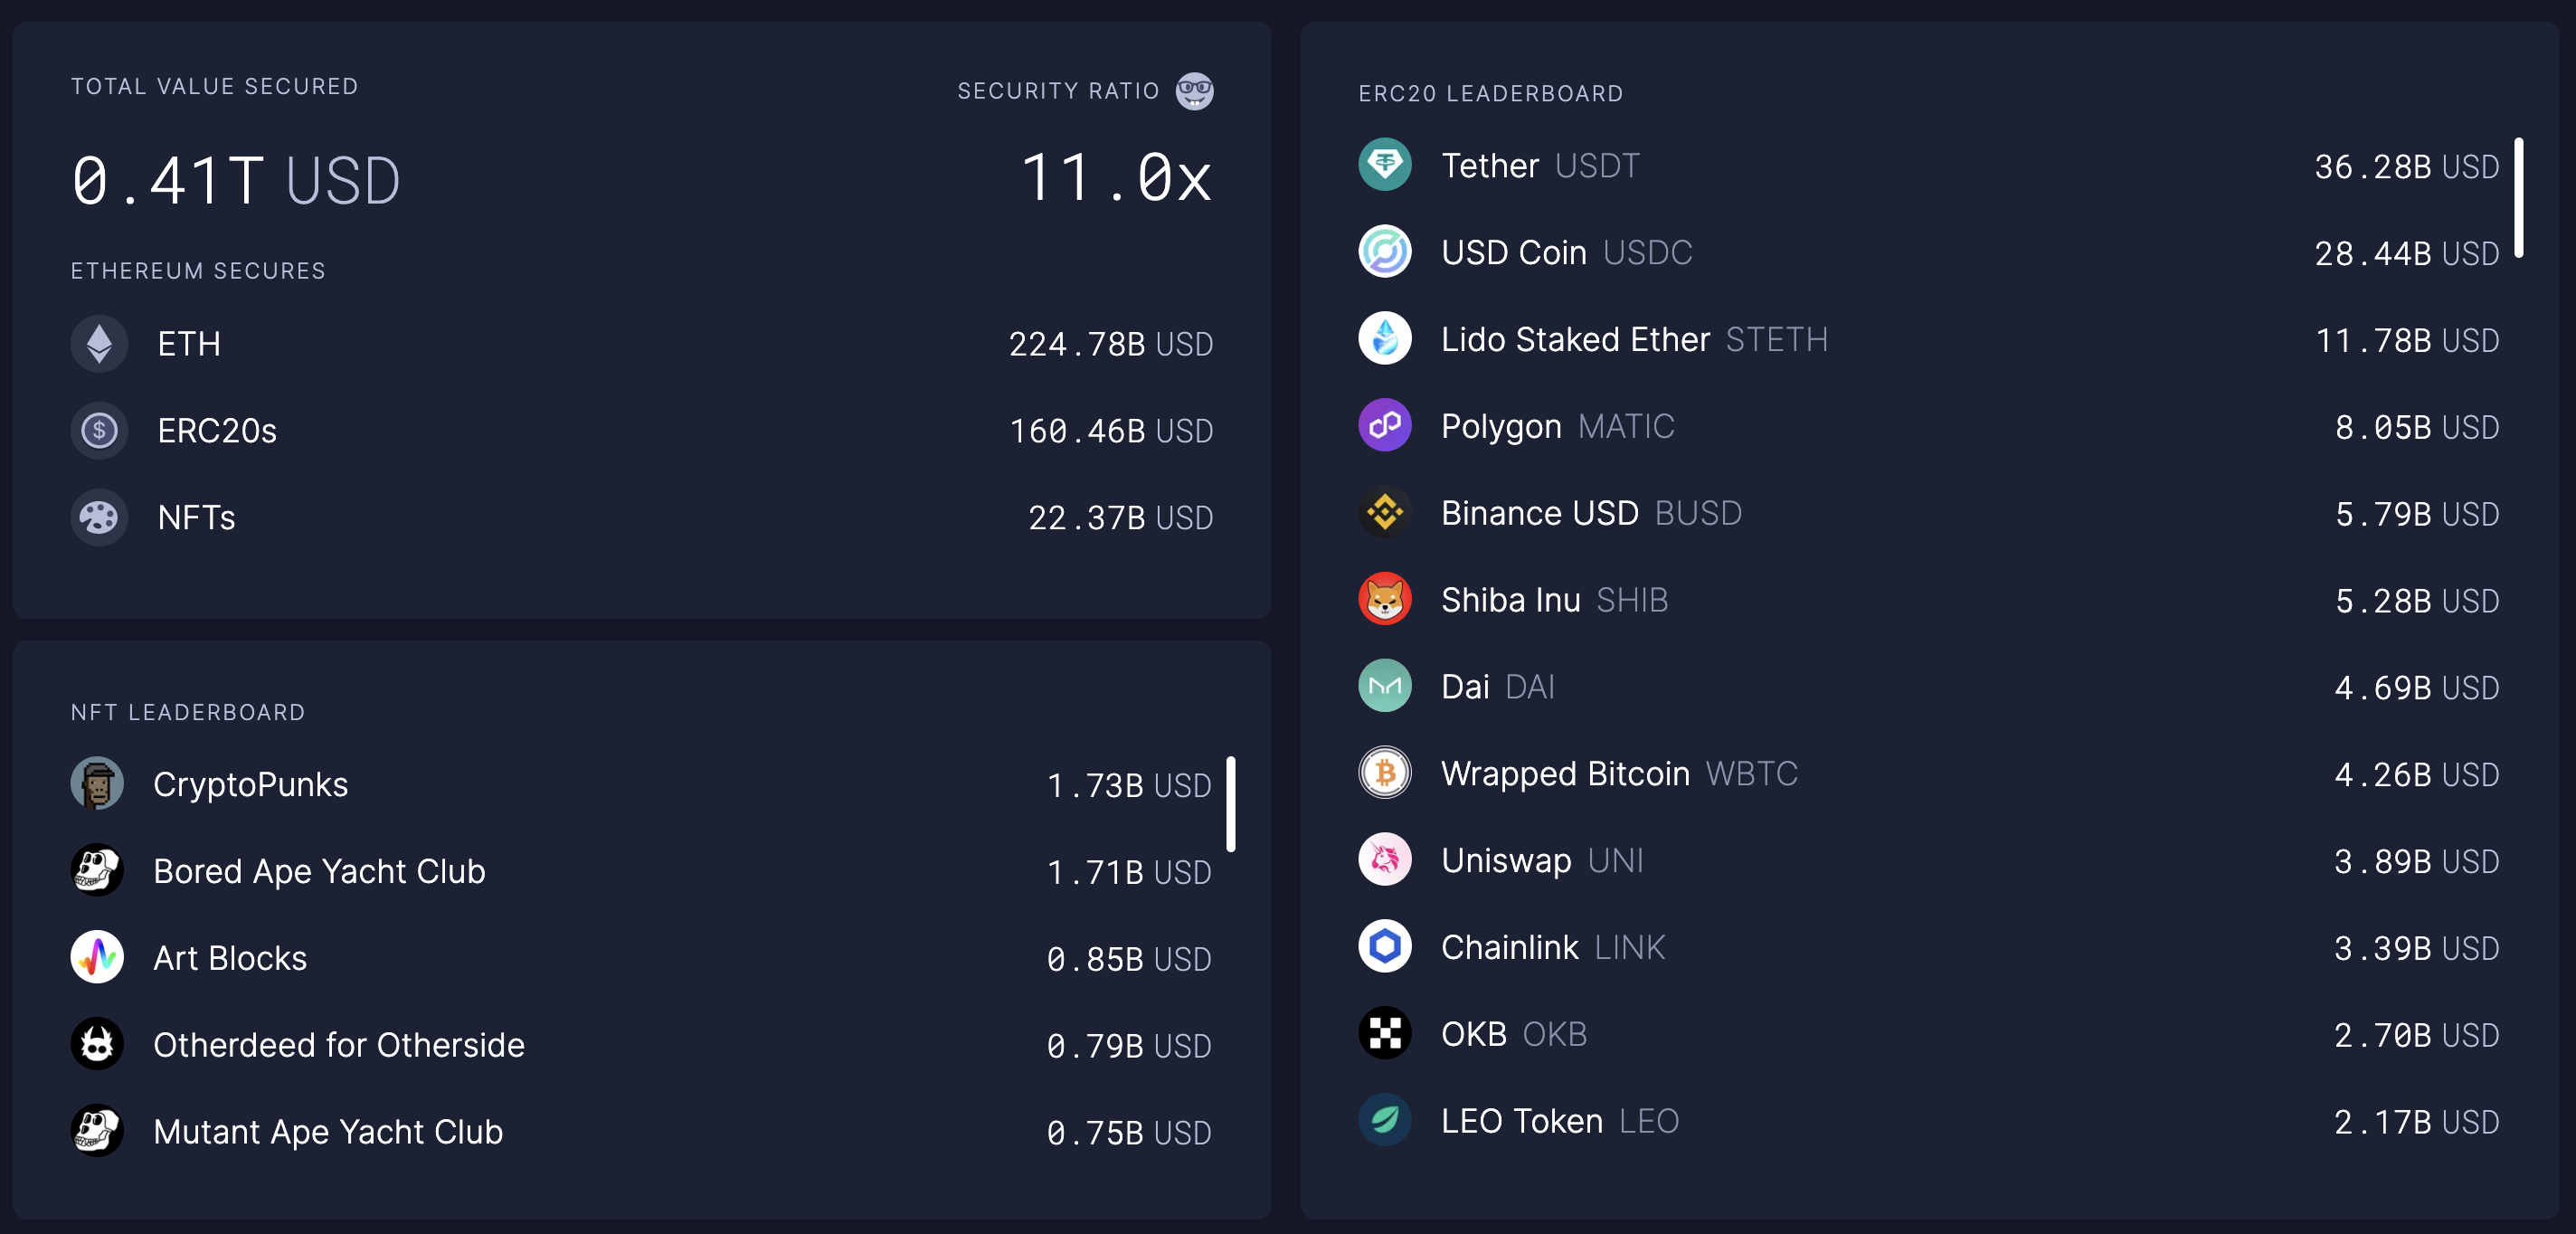
\includegraphics[width=0.9\linewidth]{images/tvs}
\caption{Statistics for total value secured (TVS), including NFT and ERC20 leaderboards, 22 May 2023}
\label{fig:tvs}
\end{center}
\end{figure}

\begin{figure}[htbp]
\begin{center}
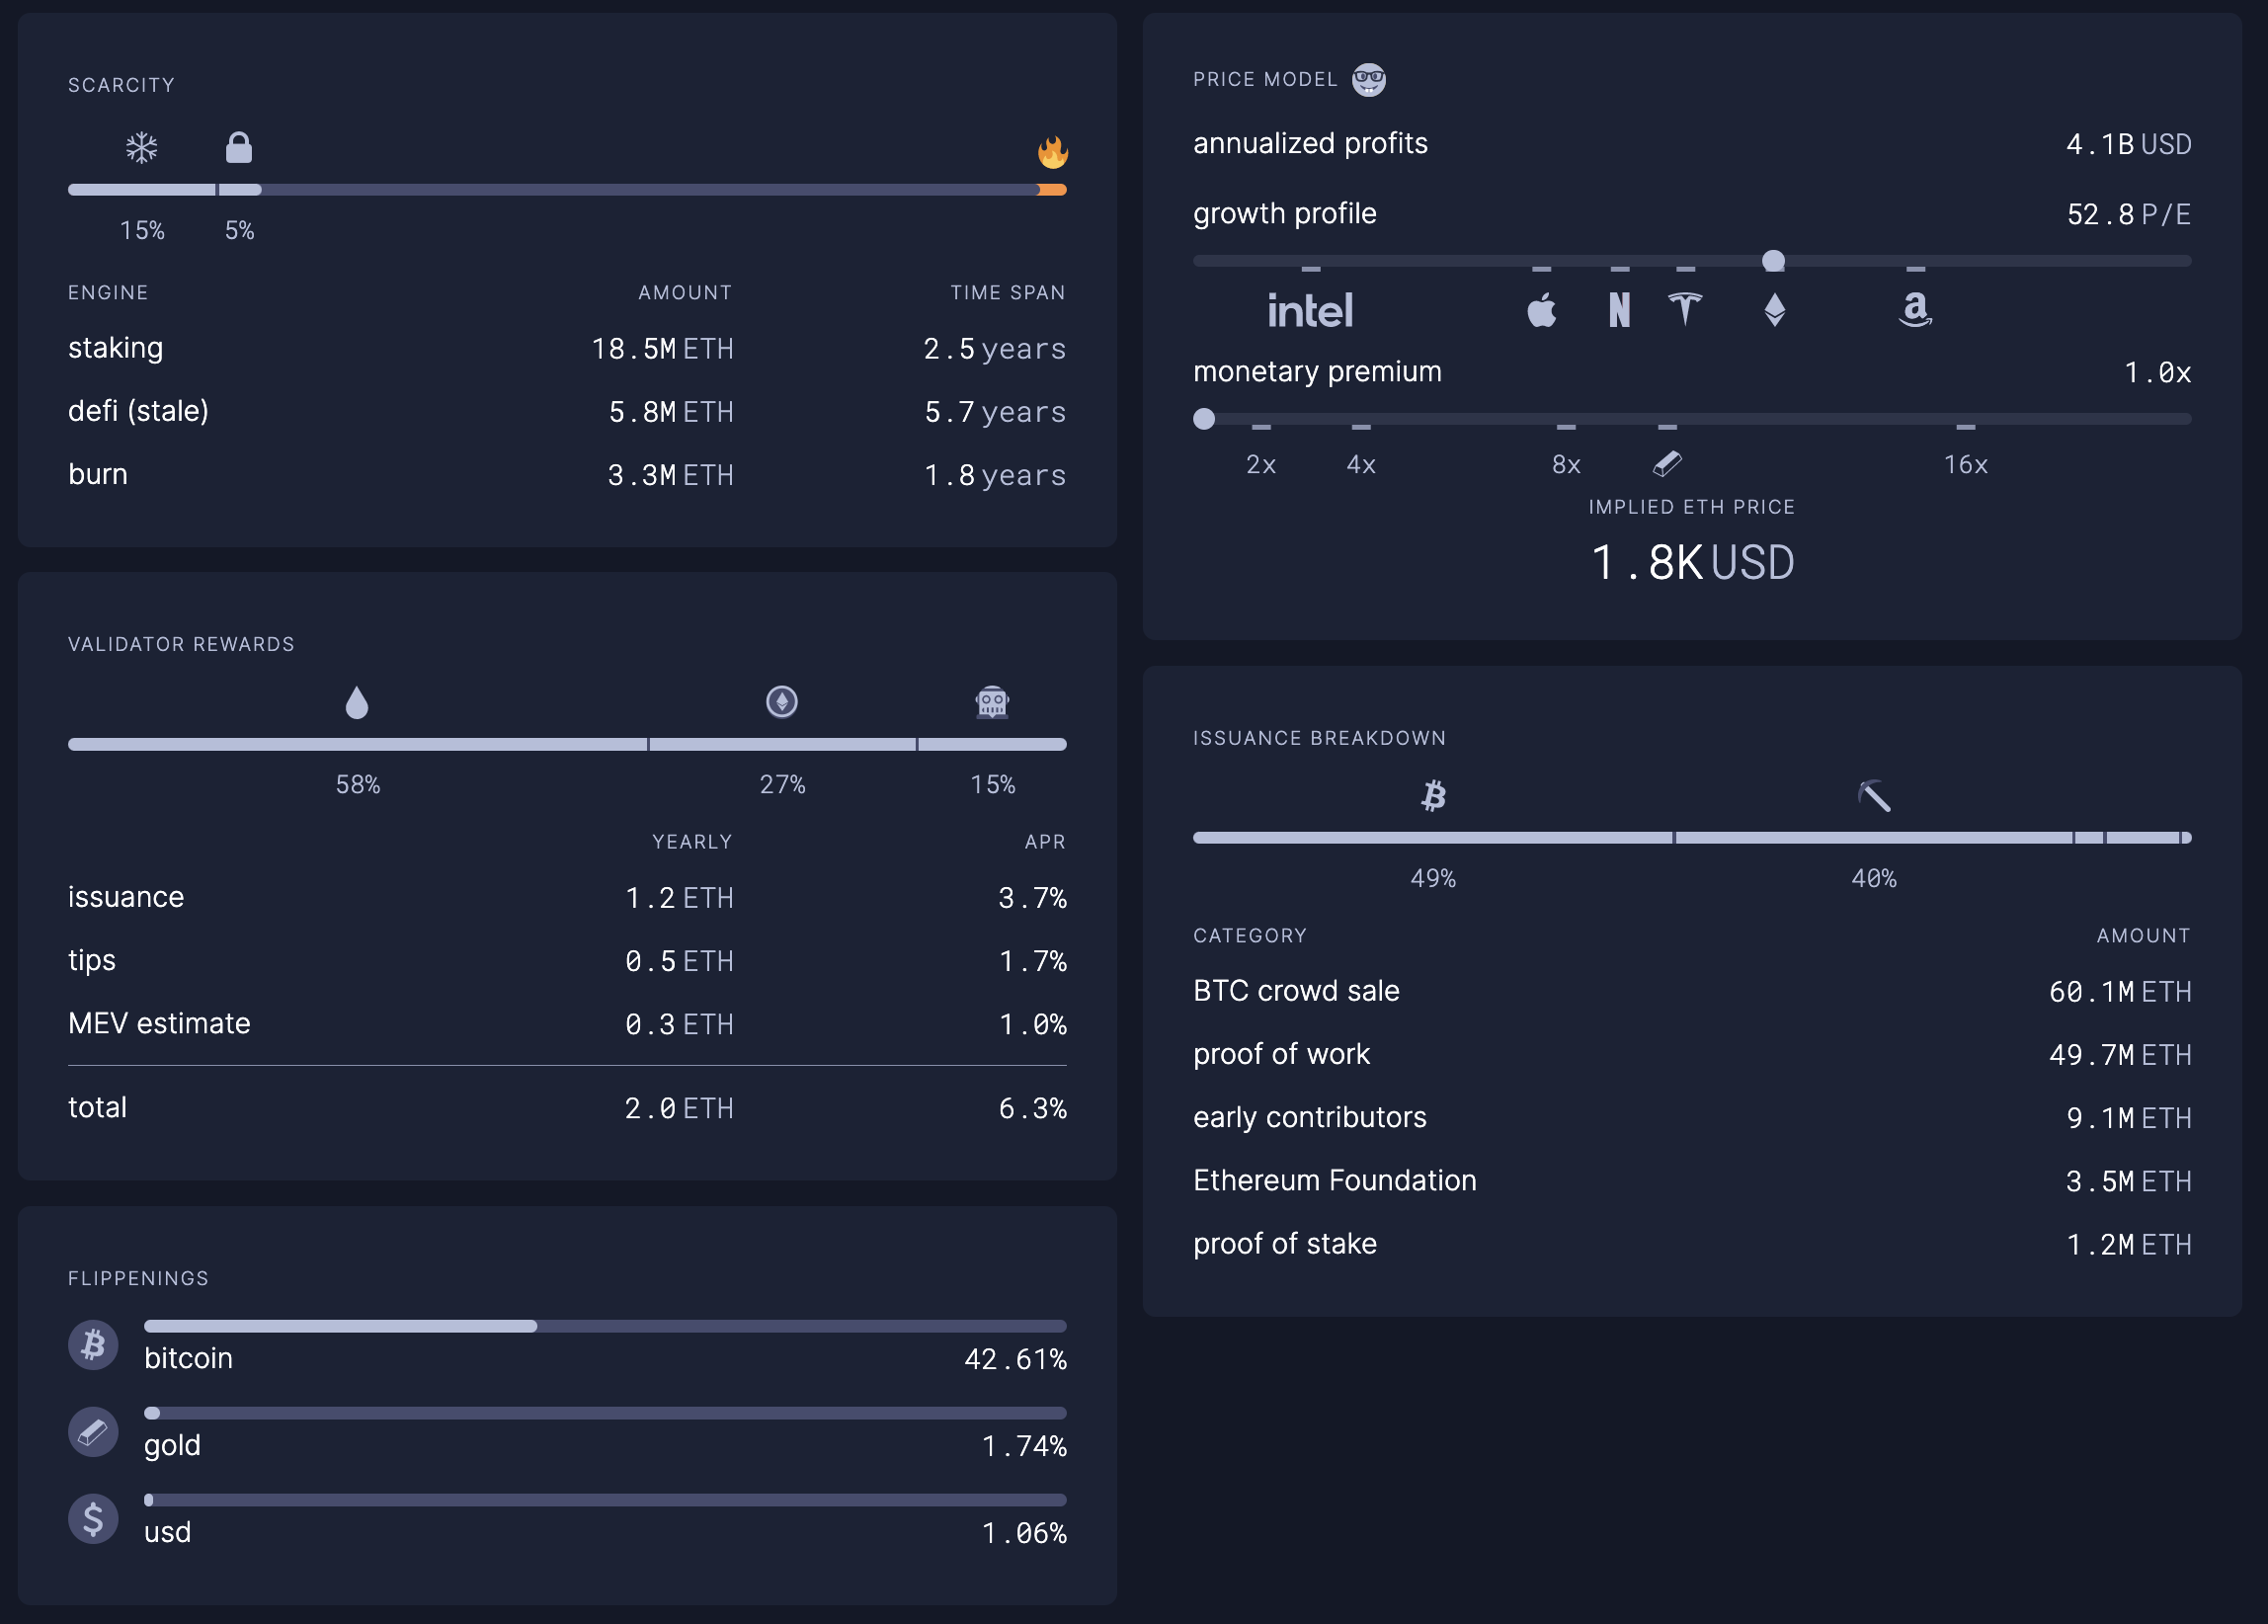
\includegraphics[width=0.9\linewidth]{images/monetary}
\caption{Monetary premium shows Scarcity (staking, defi, burn), Validator rewards (issuance, tips, mev, Flippenings (bitcoin, gold and usd), Issuance breakdown by category and an interactive price model based on selected growth profile and monetary premium, 22 May 2023}
\label{fig:monetary}
\end{center}
\end{figure}
\clearpage


% --------------------------------------
\subsubsection*{Rated network explorer}
% --------------------------------------
\textbf{Entity Views} \\
% ----------------------------------
\begin{figure}[htbp]
\begin{center}
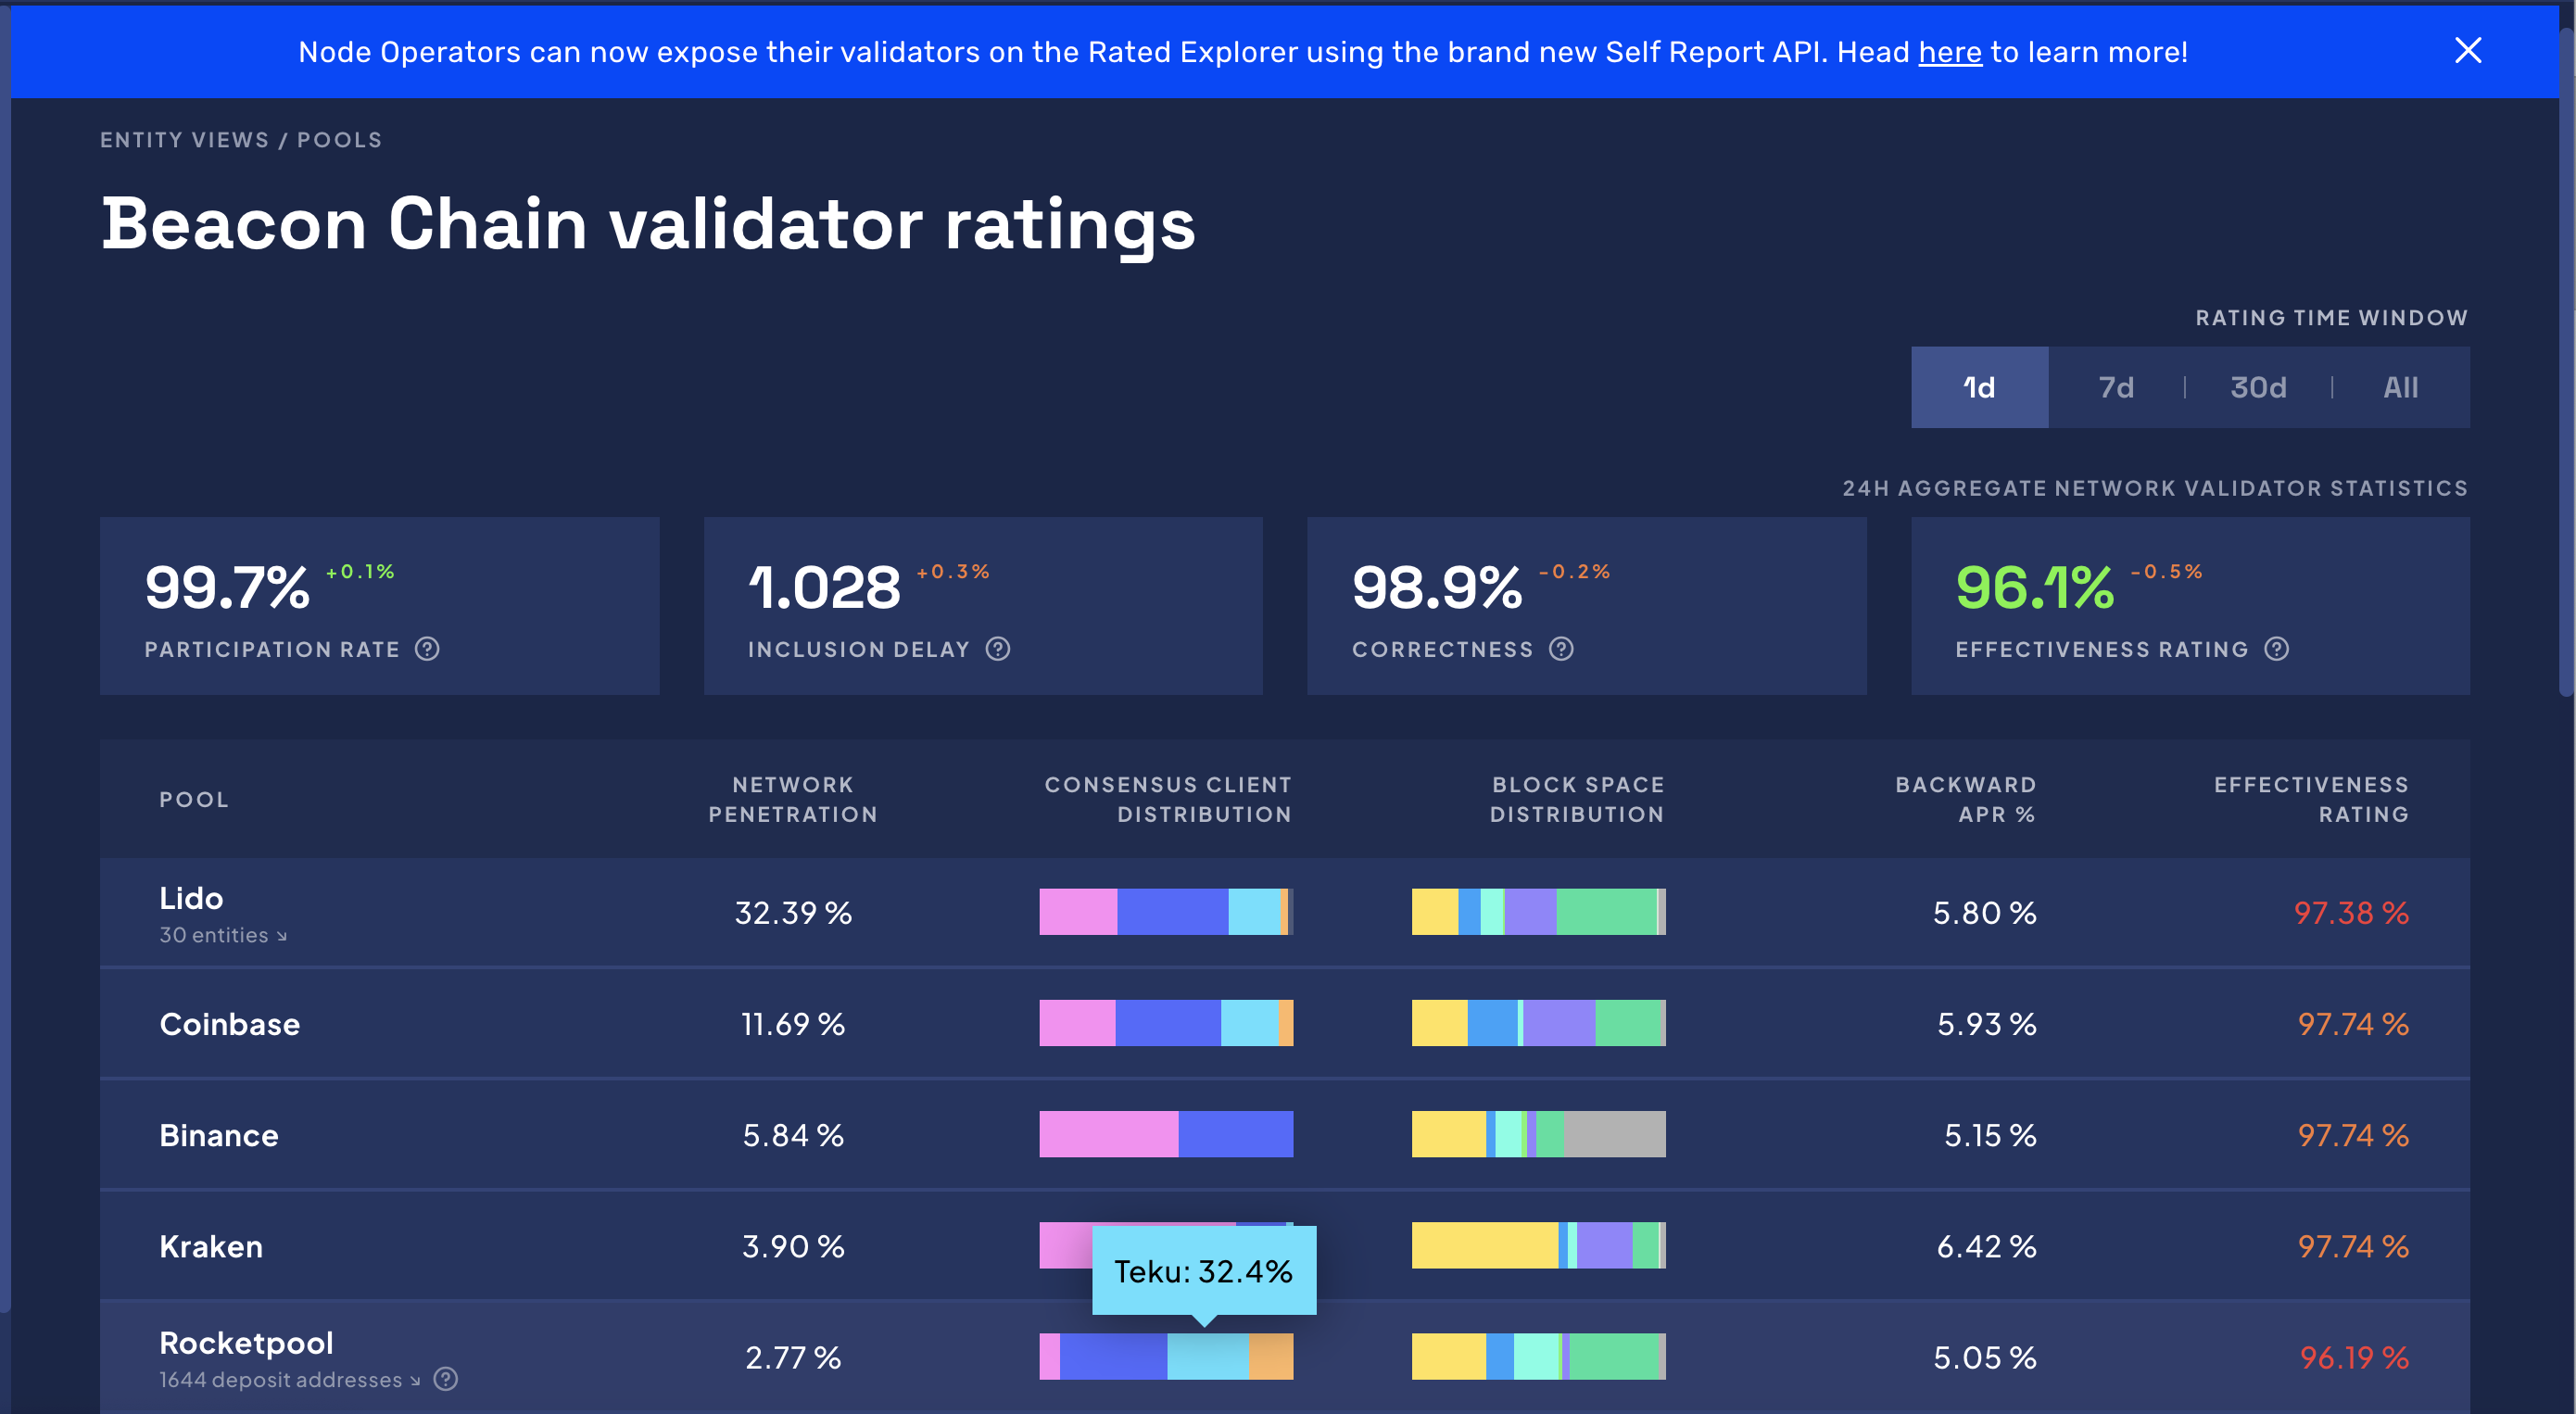
\includegraphics[width=\linewidth]{images/ratedentity1}
\caption{Rated network explorer: beacon chain validator ratings for staking pools. Select from timeframes: 1 day, 7 days, 30 days, or all (since merge) , 1 June 2023}
\label{fig:ratedentity1}
\end{center}
\end{figure}

\begin{figure}[htbp]
\begin{center}
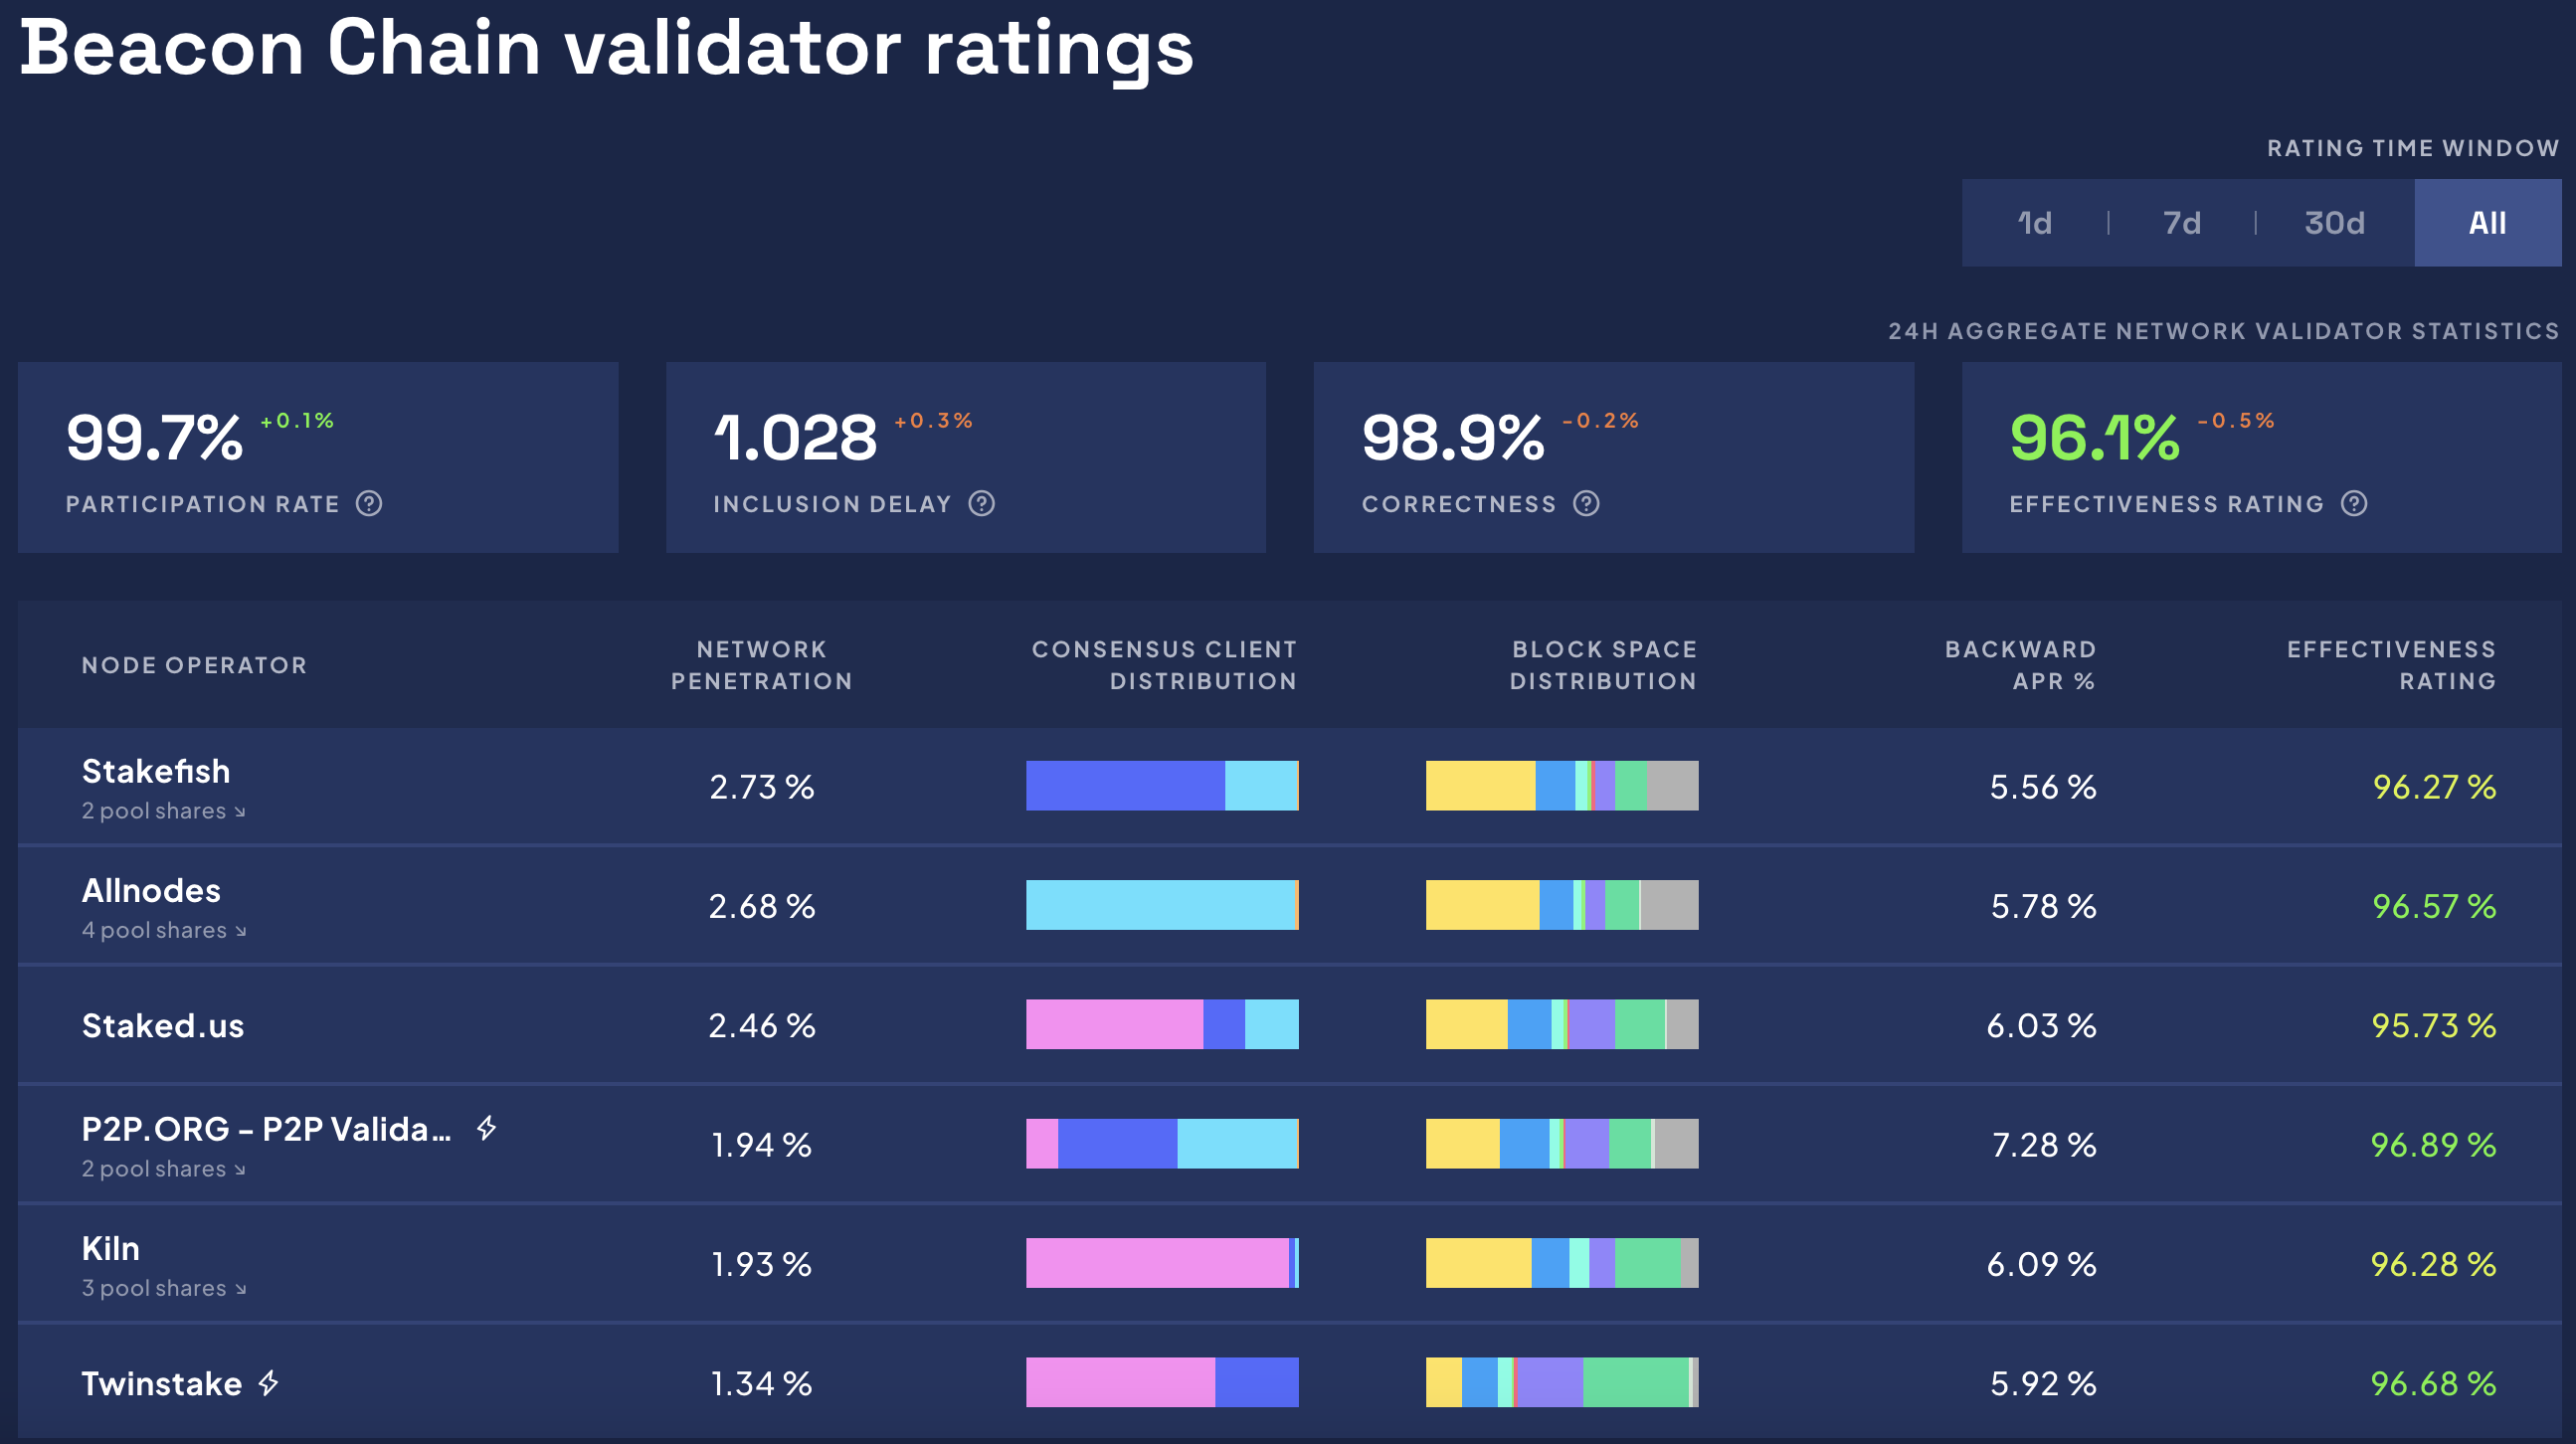
\includegraphics[width=\linewidth]{images/ratedentity2}
\caption{Rated network explorer: beacon chain validator ratings for node operators. Select from timeframes: 1 day, 7 days, 30 days, or all (since merge) , 1 June 2023}
\label{fig:ratedentity2}
\end{center}
\end{figure}

\begin{figure}[htbp]
\begin{center}
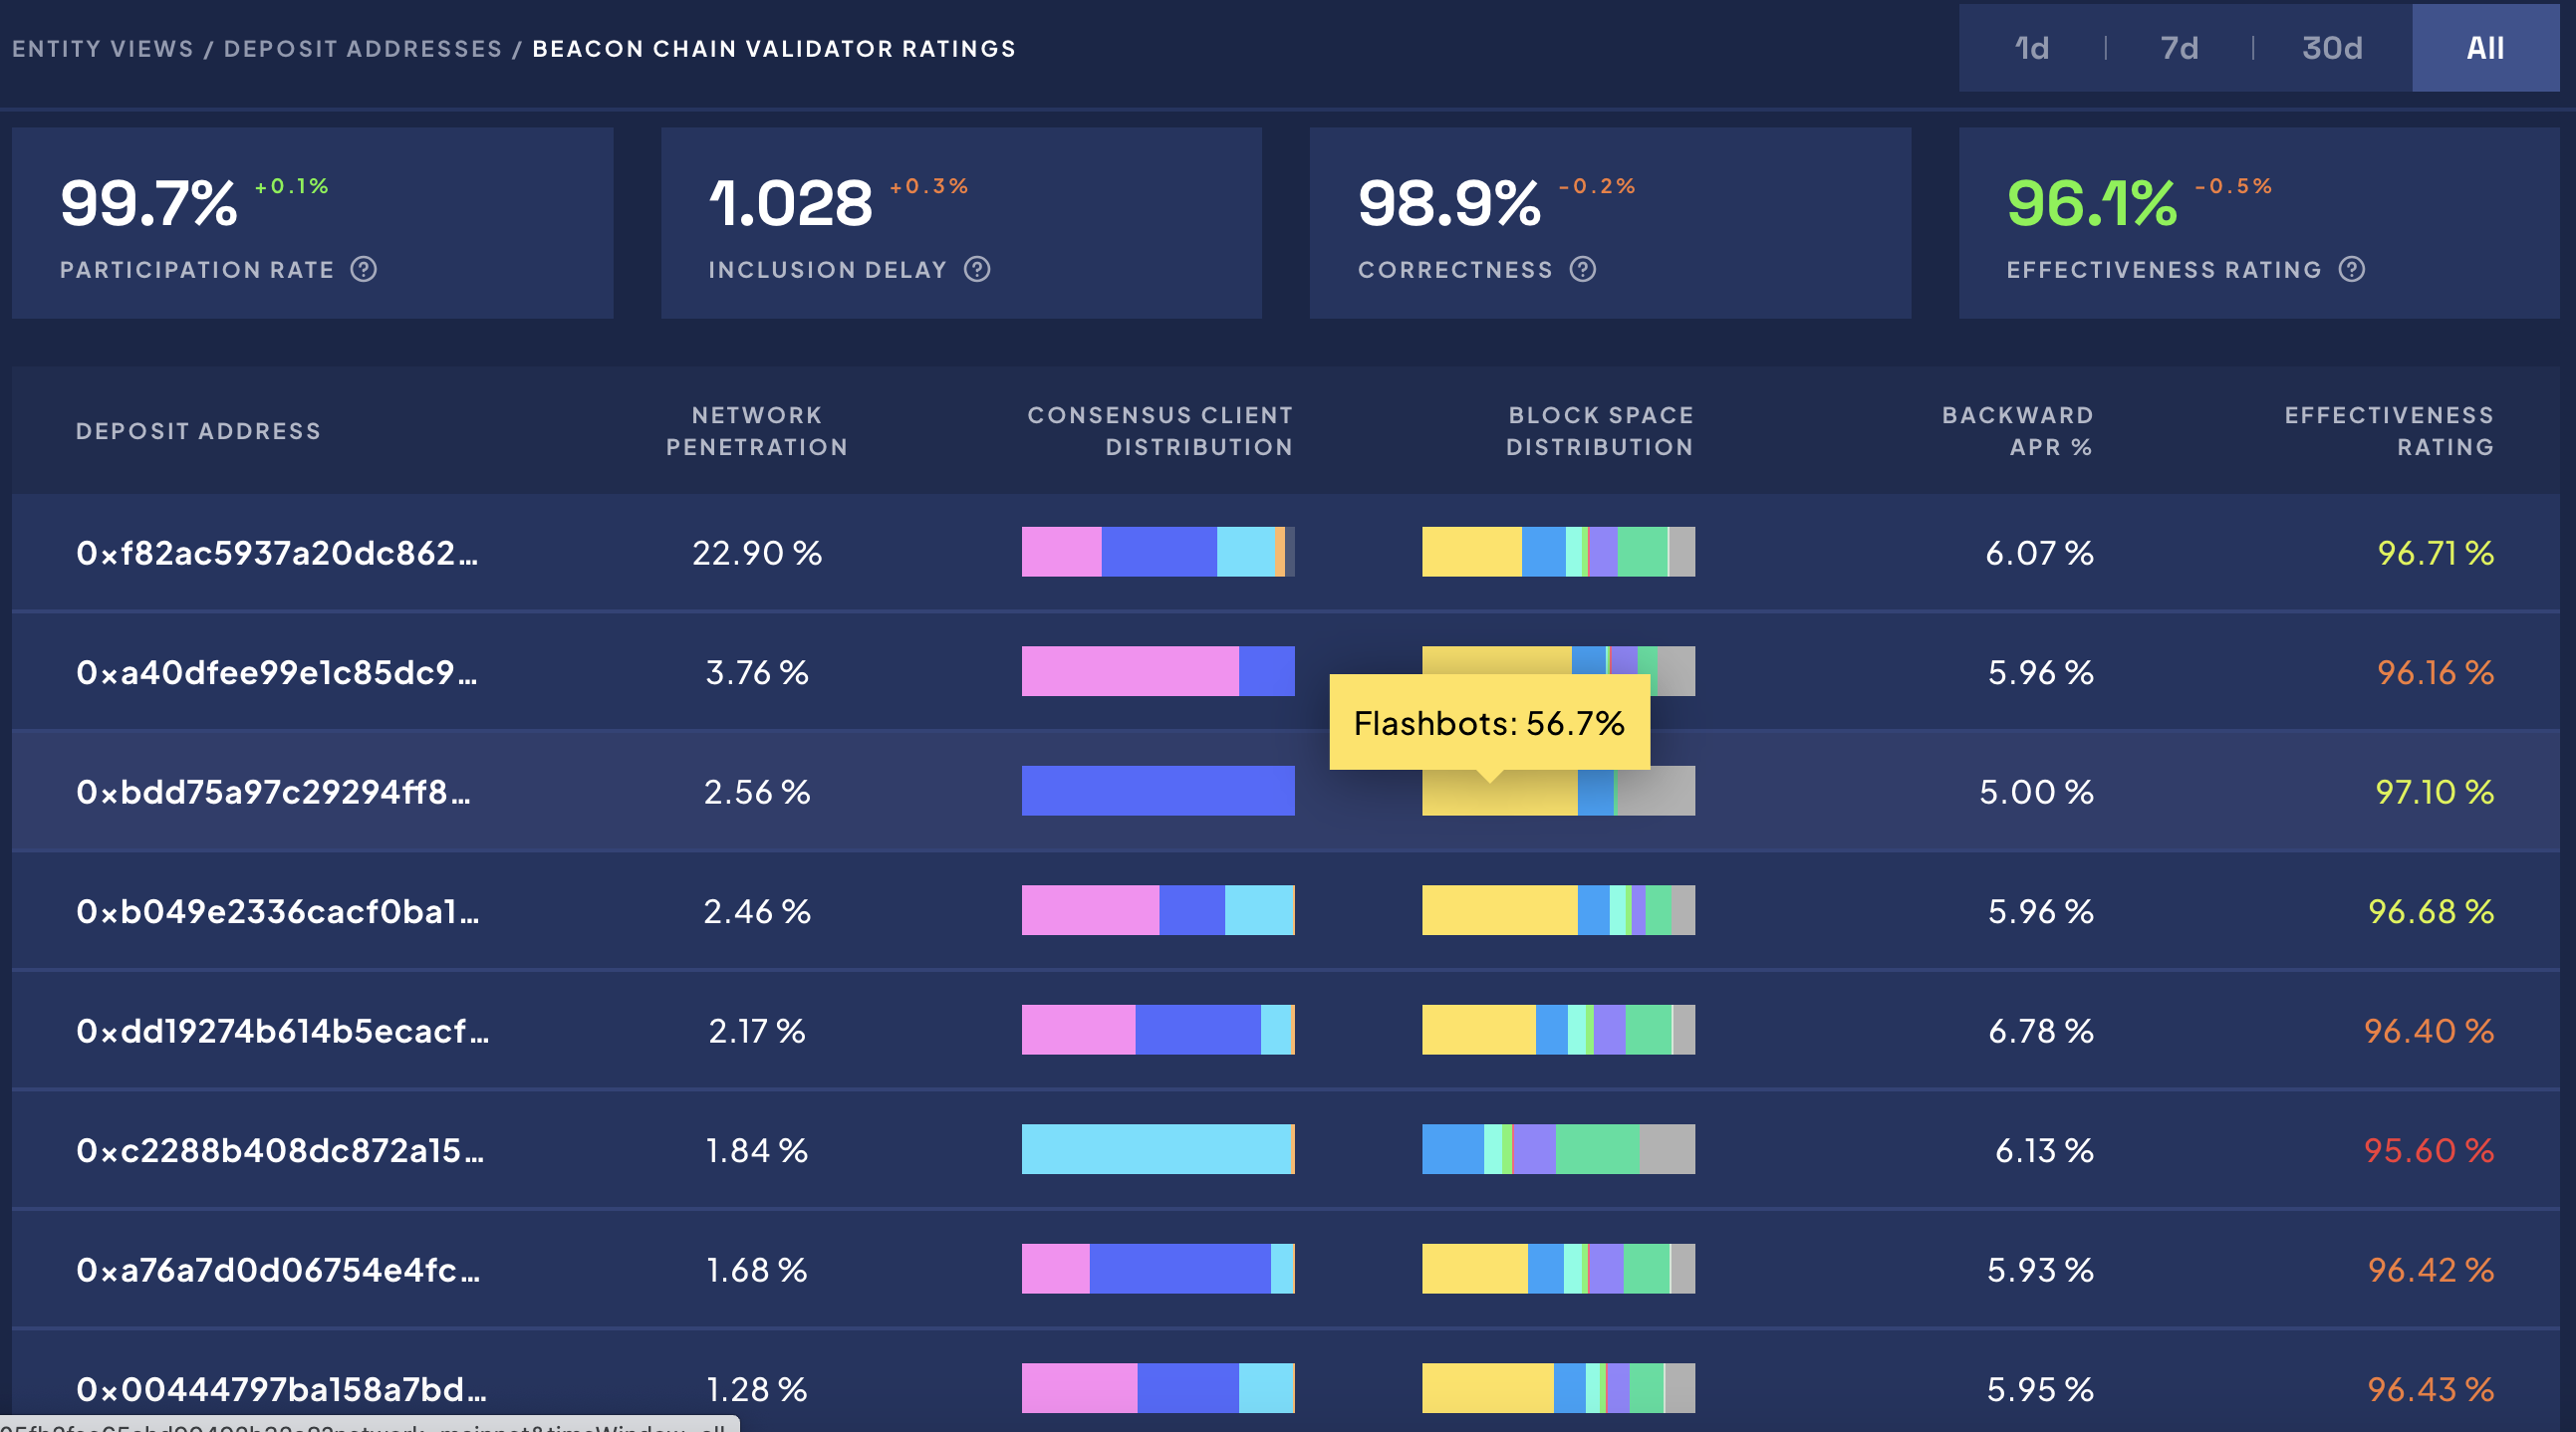
\includegraphics[width=\linewidth]{images/ratedentity3}
\caption{Rated network explorer: beacon chain validator ratings by deposit addresses. Select from timeframes: 1 day, 7 days, 30 days, or all (since merge) , 1 June 2023}
\label{fig:ratedentity3}
\end{center}
\end{figure}

\begin{figure}[htbp]
\begin{center}
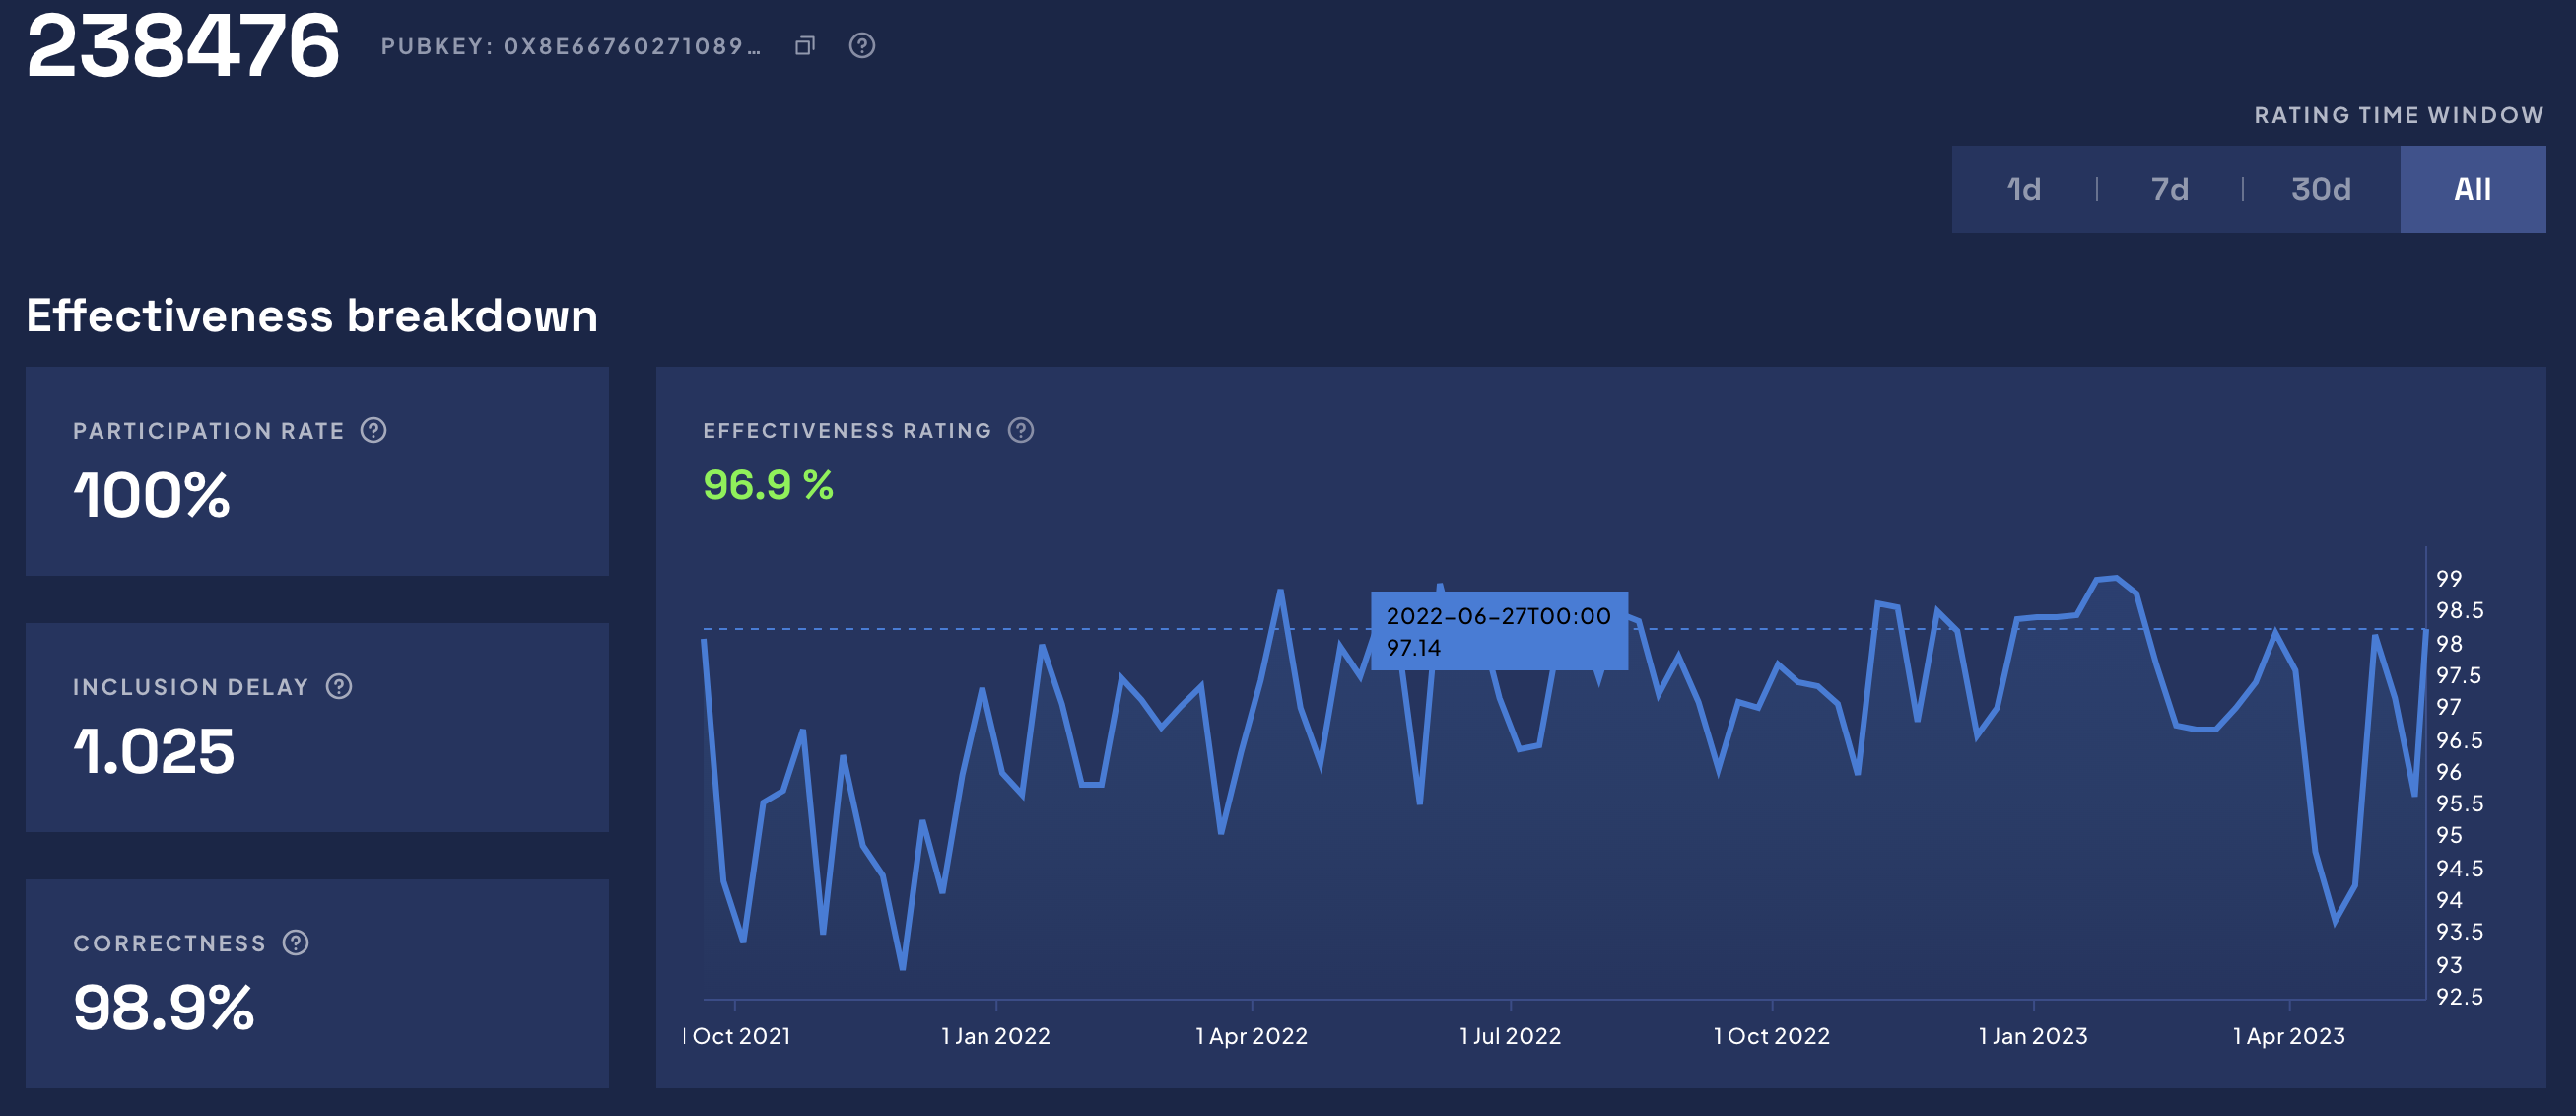
\includegraphics[width=\linewidth]{images/ratedentity4a}\\
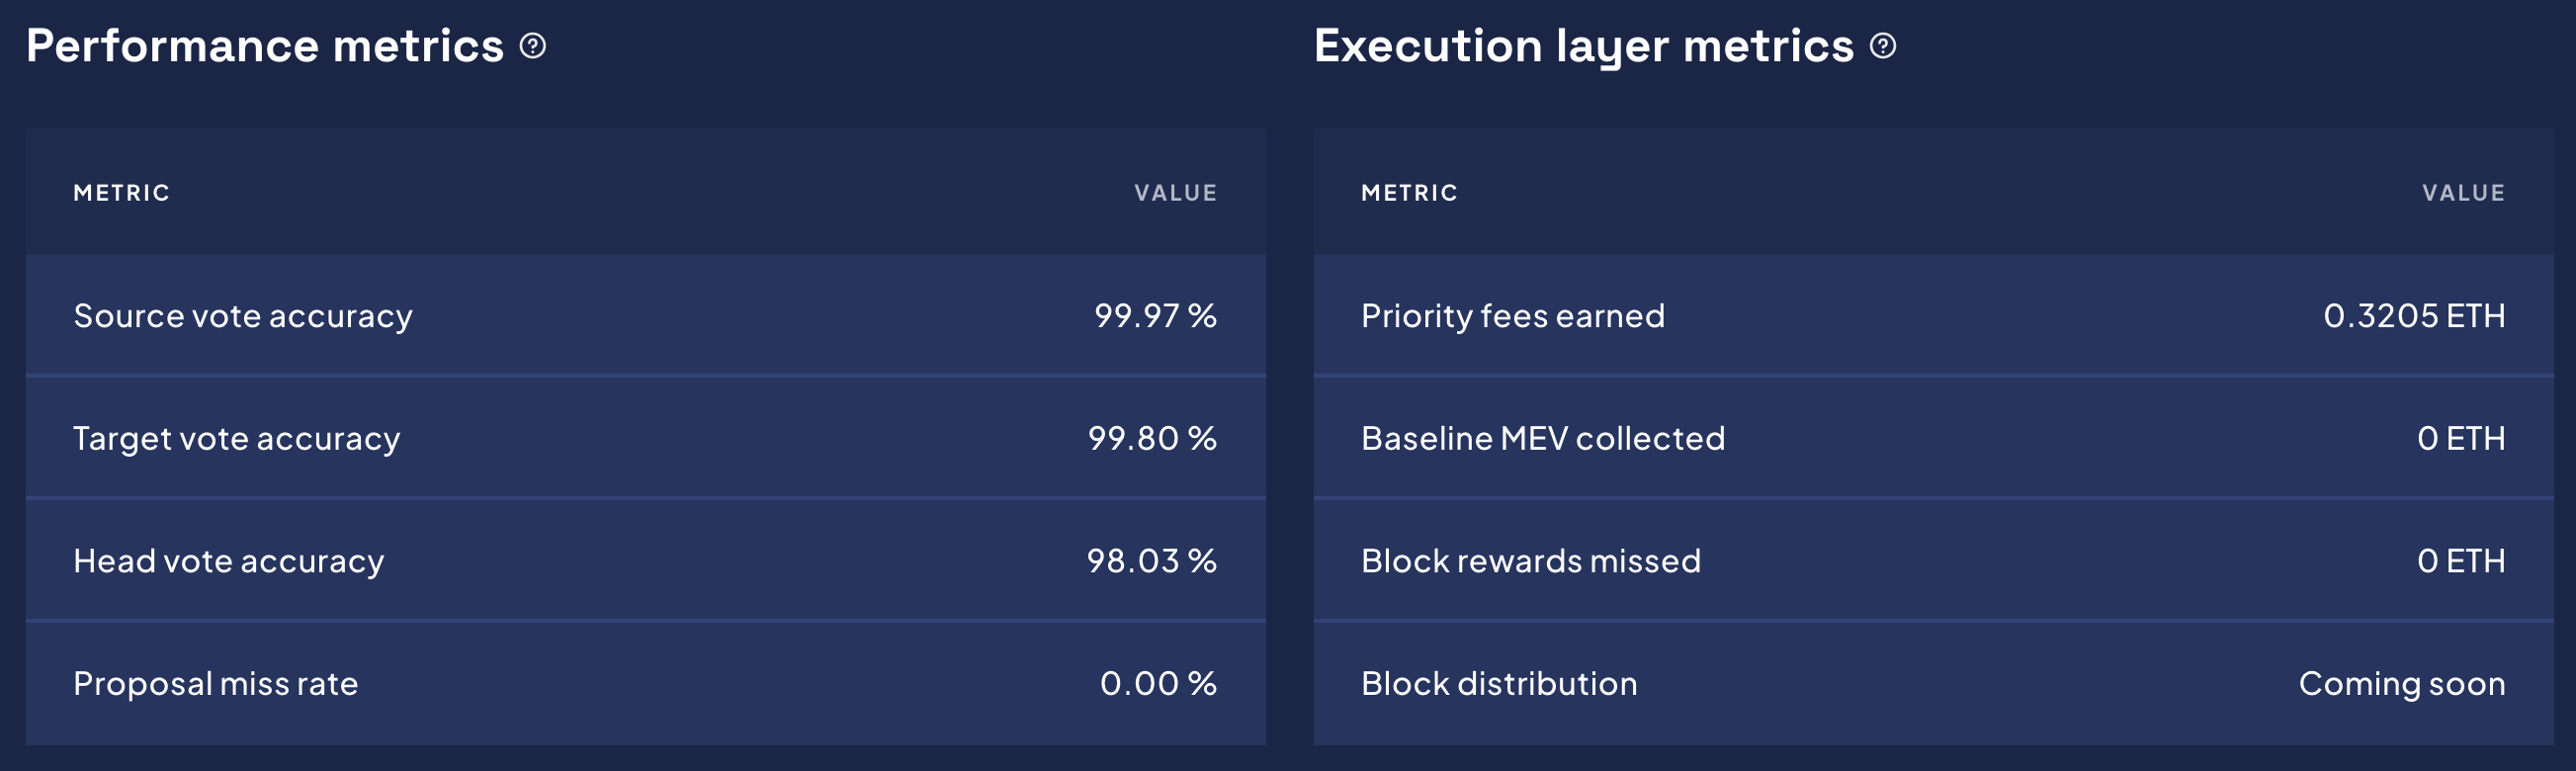
\includegraphics[width=\linewidth]{images/ratedentity4b}\\
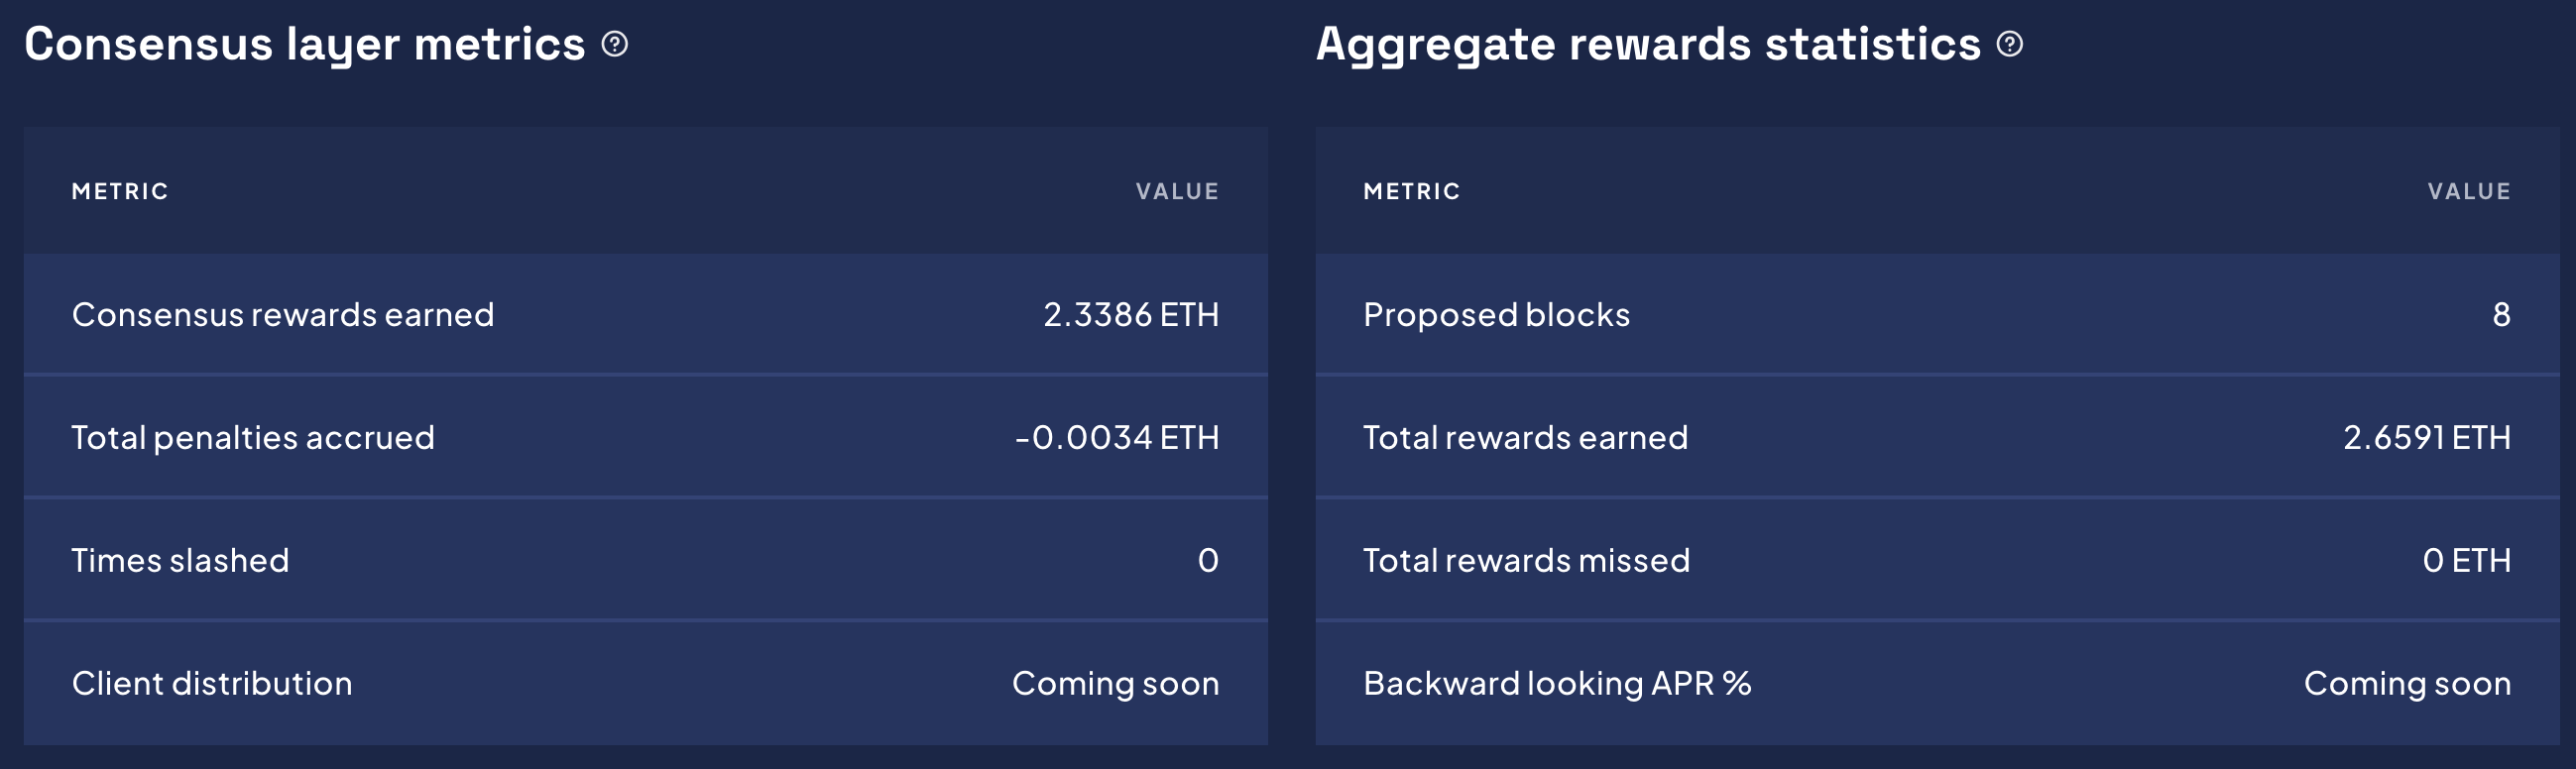
\includegraphics[width=\linewidth]{images/ratedentity4c}
\caption{Rated network explorer: view of a chosen validator (using id or public key). Select from timeframes: 1 day, 7 days, 30 days, or all (since merge) , 1 June 2023}
\label{fig:ratedentity4}
\end{center}
\end{figure}
\clearpage

\textbf{Aggregate Views} 
% ----------------------------------
\begin{figure}[htbp]
\begin{center}
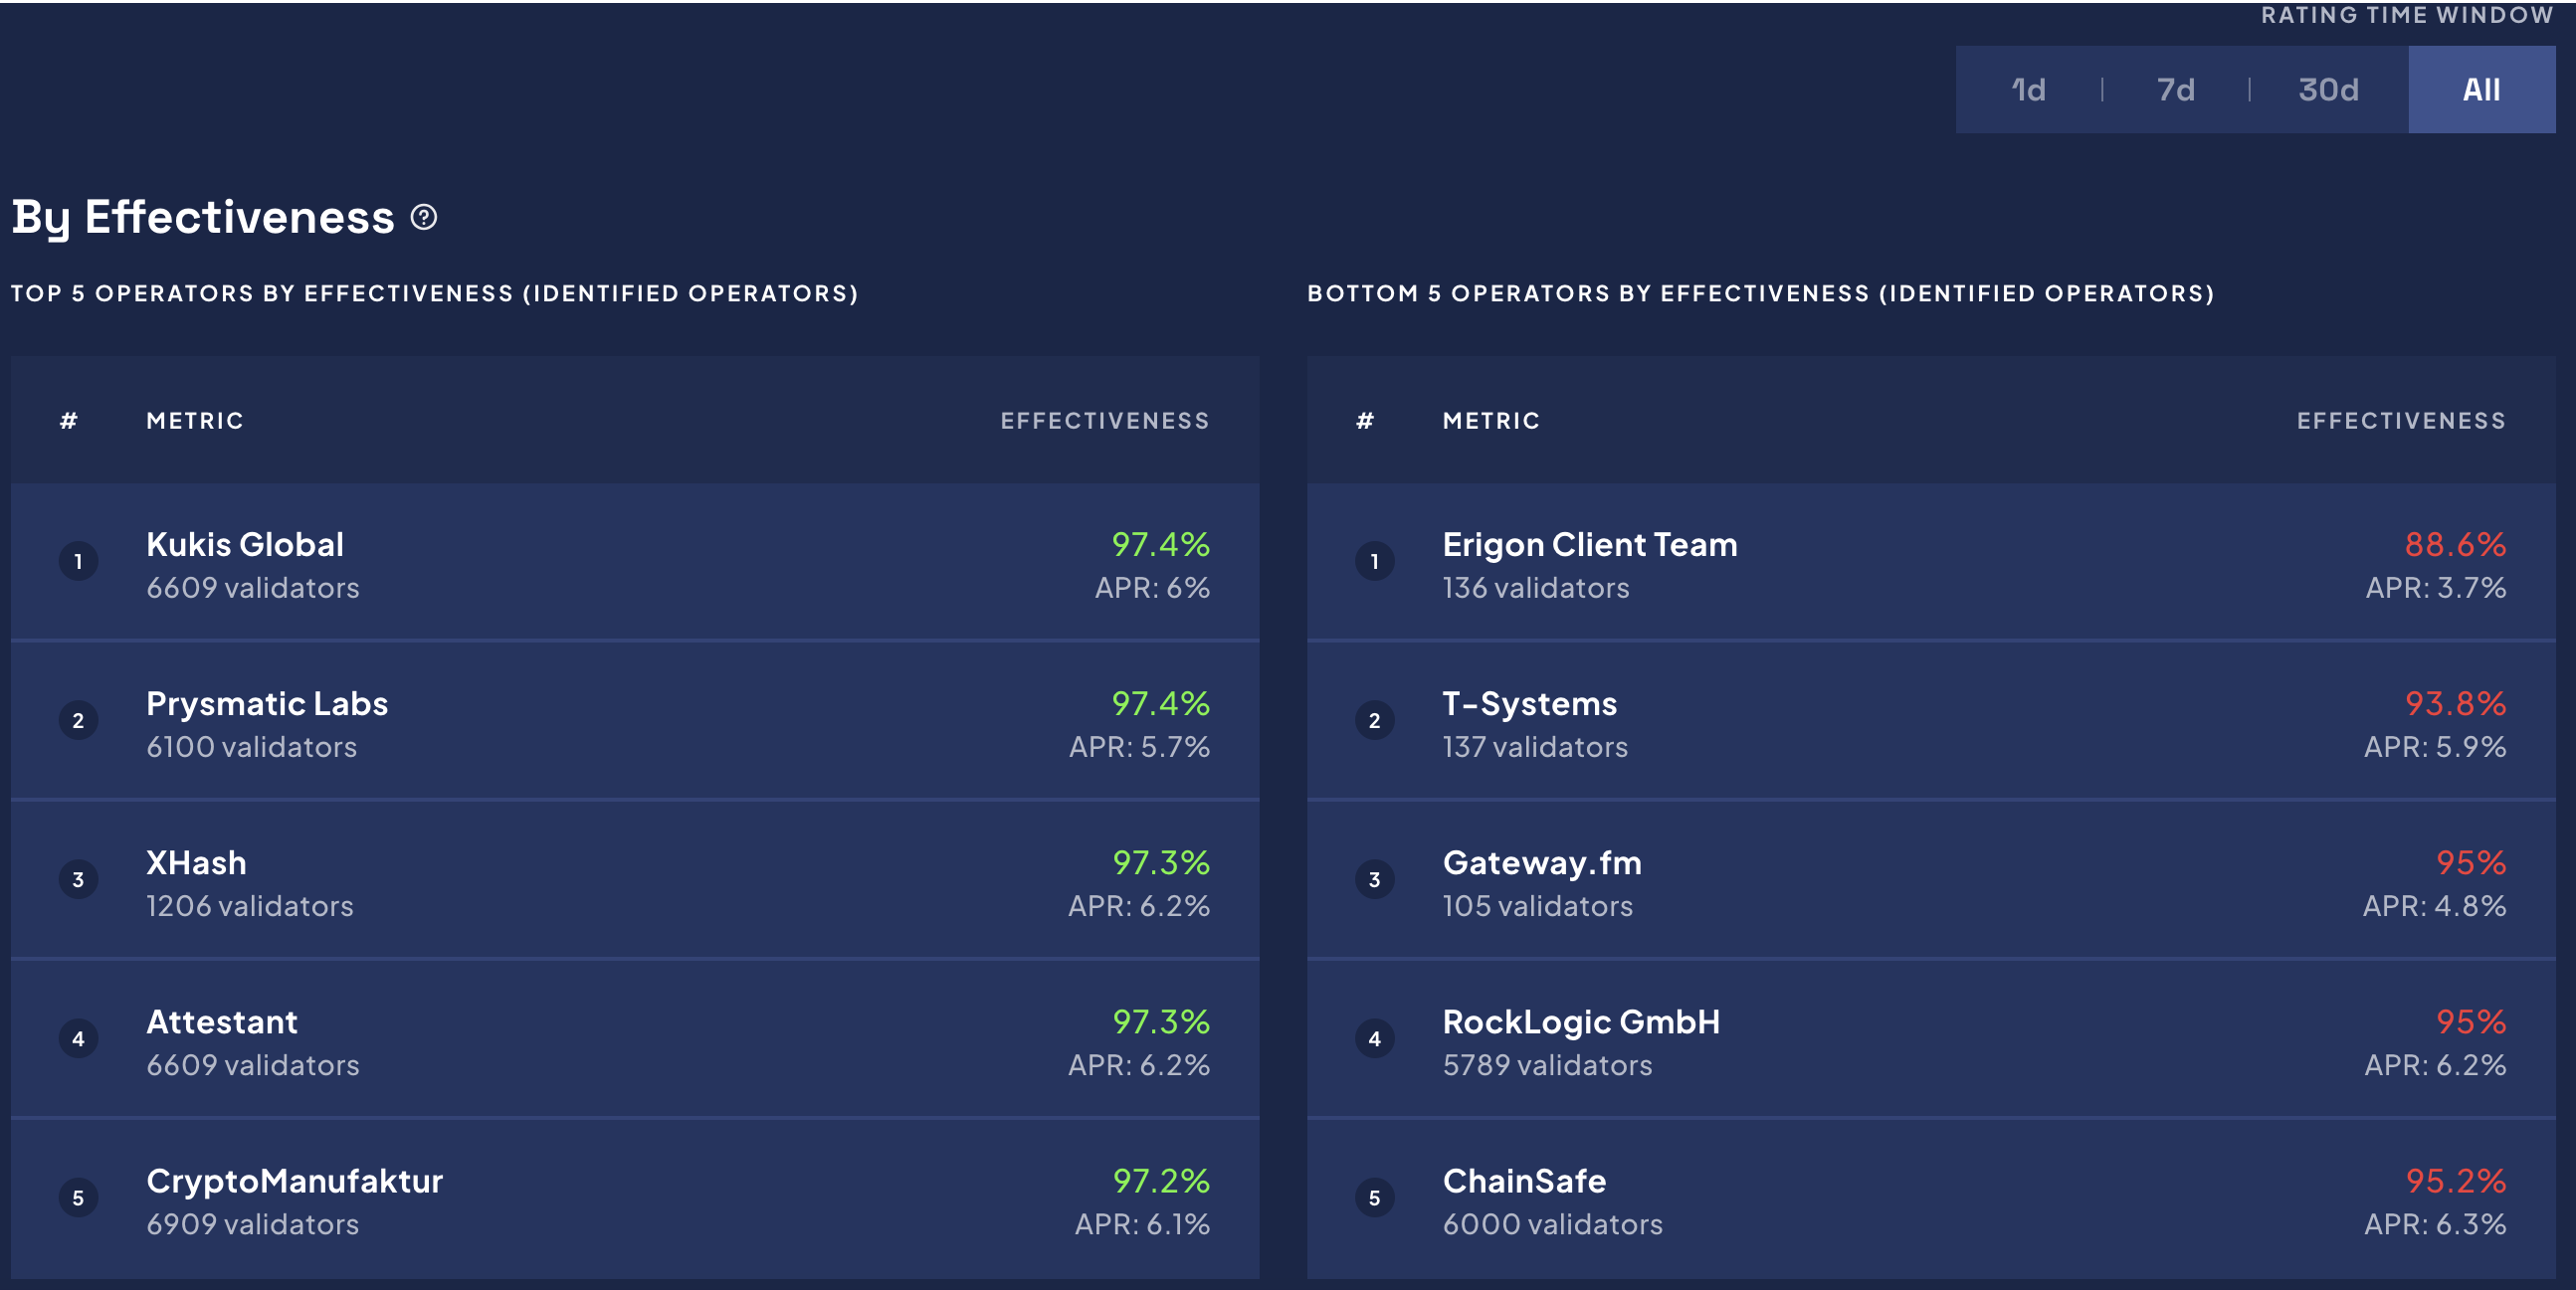
\includegraphics[width=\linewidth]{images/ratedtrend1}\\
(a)
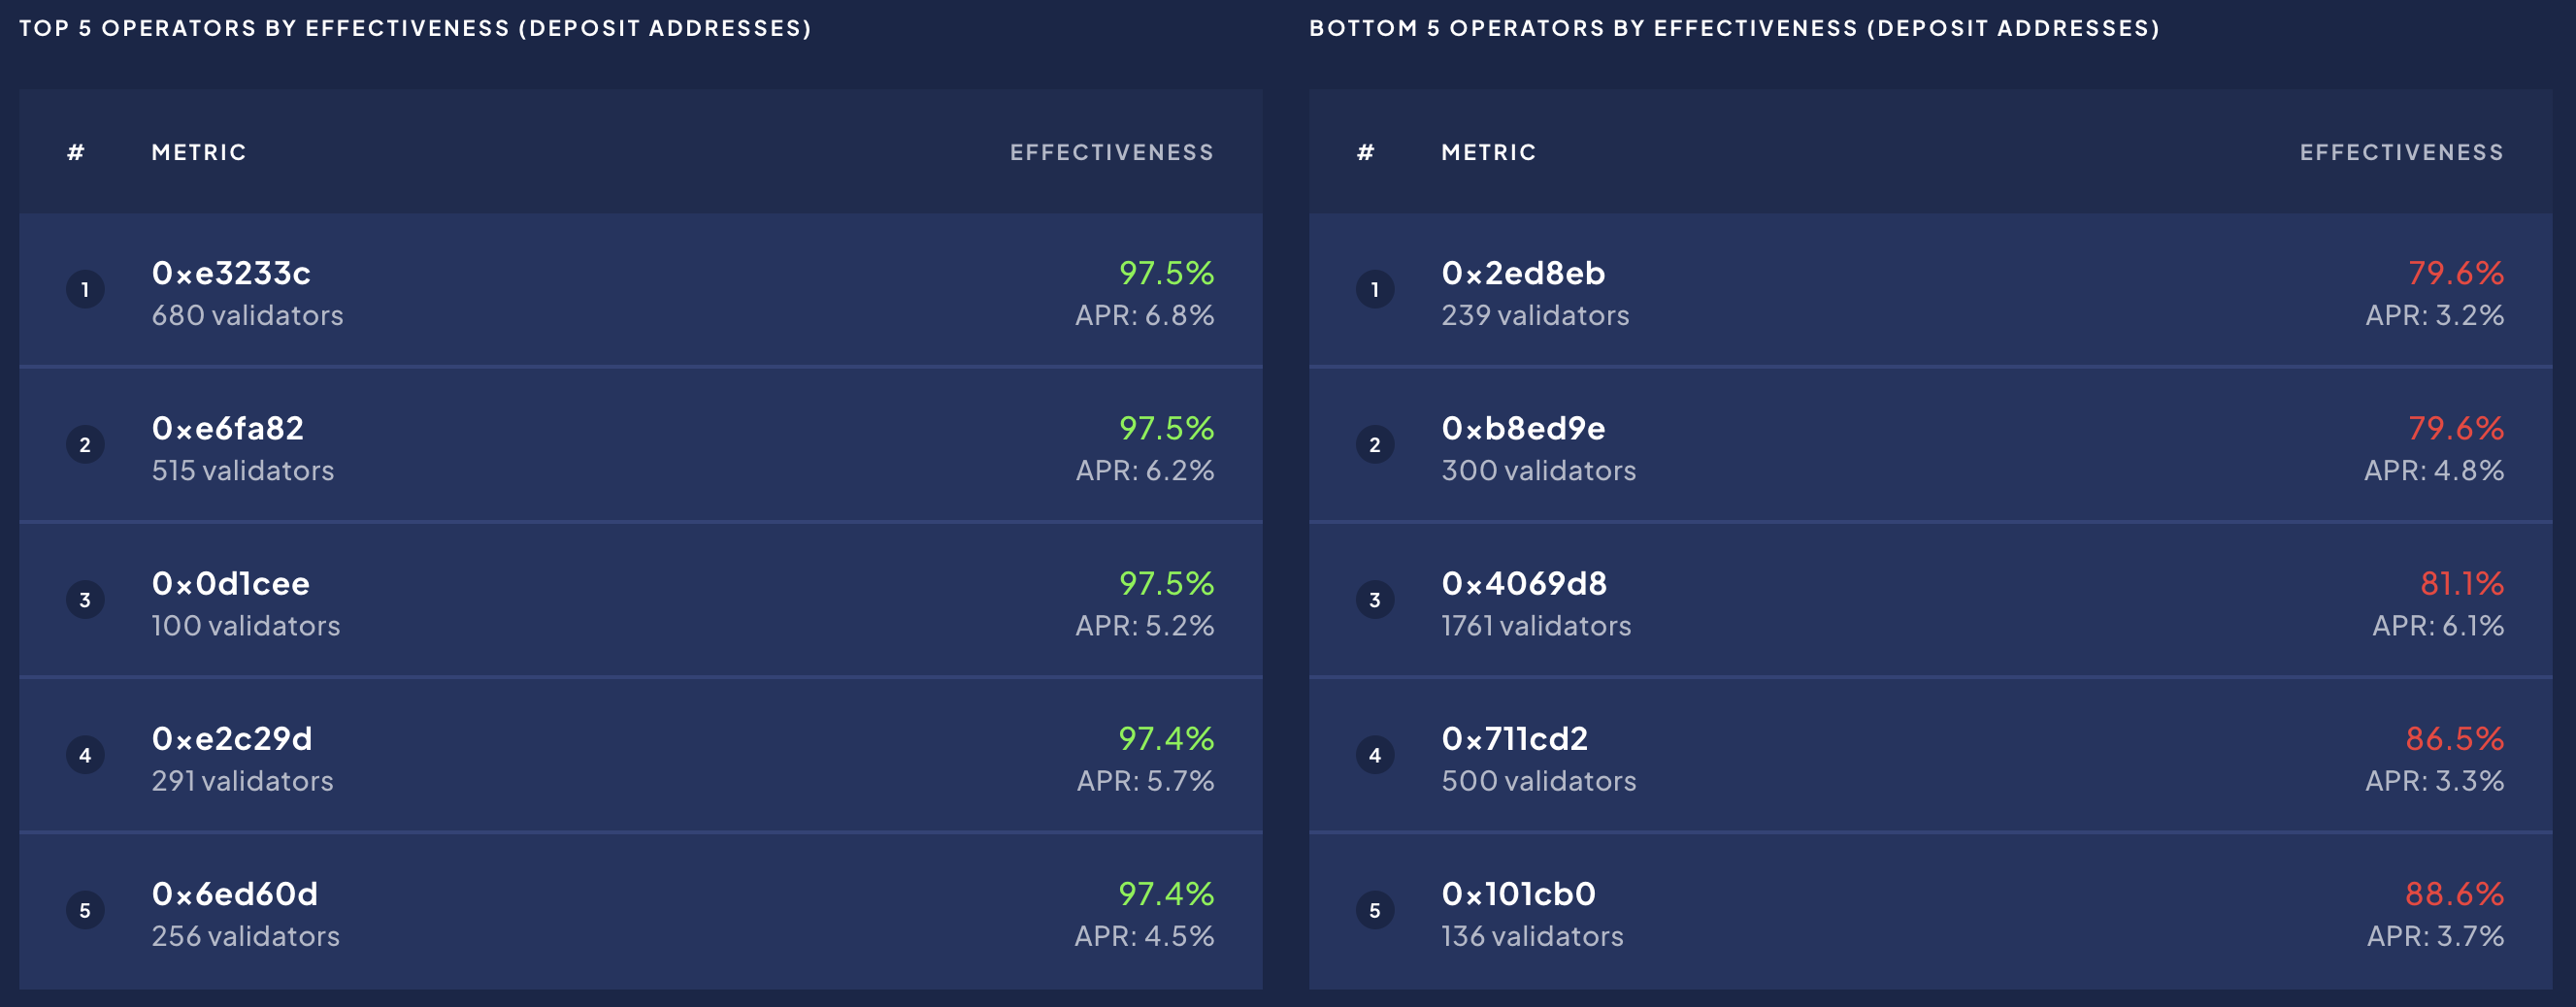
\includegraphics[width=\linewidth]{images/ratedtrend2}\\
(b)
\caption{Rated network explorer: top 5 and bottom 5 identified operators (a) and the top and bottom 5 operators by deposit addresses (b). Timeframes: 1 day, 7 days, 30 days or all (since merge), 1 June 2023}
\label{fig:ratedtrend1}
\end{center}
\end{figure}

\begin{figure}[htbp]
\begin{center}
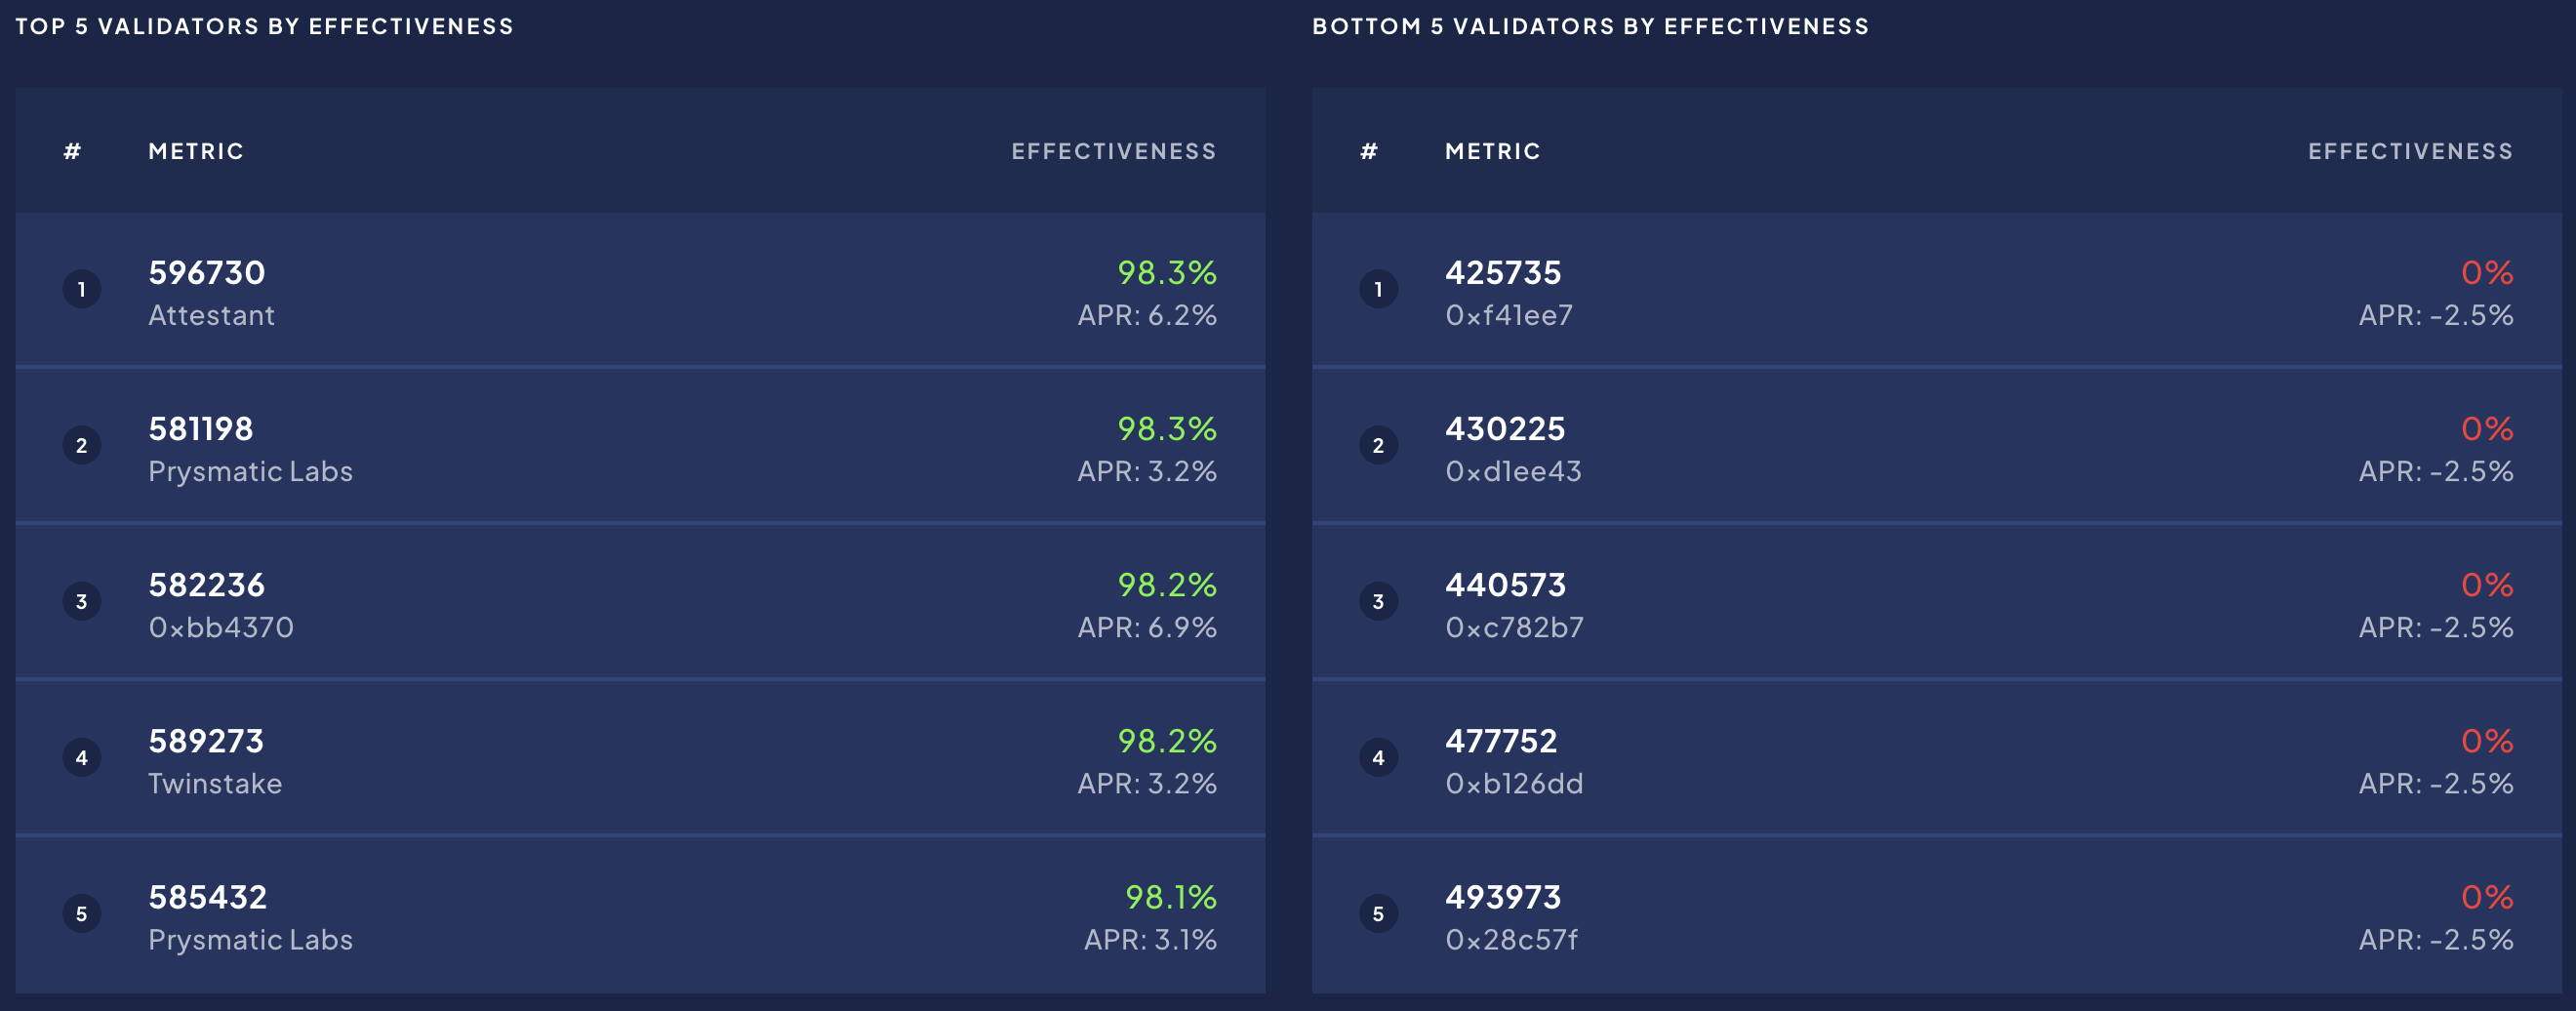
\includegraphics[width=\linewidth]{images/ratedtrend3}\\
(a)
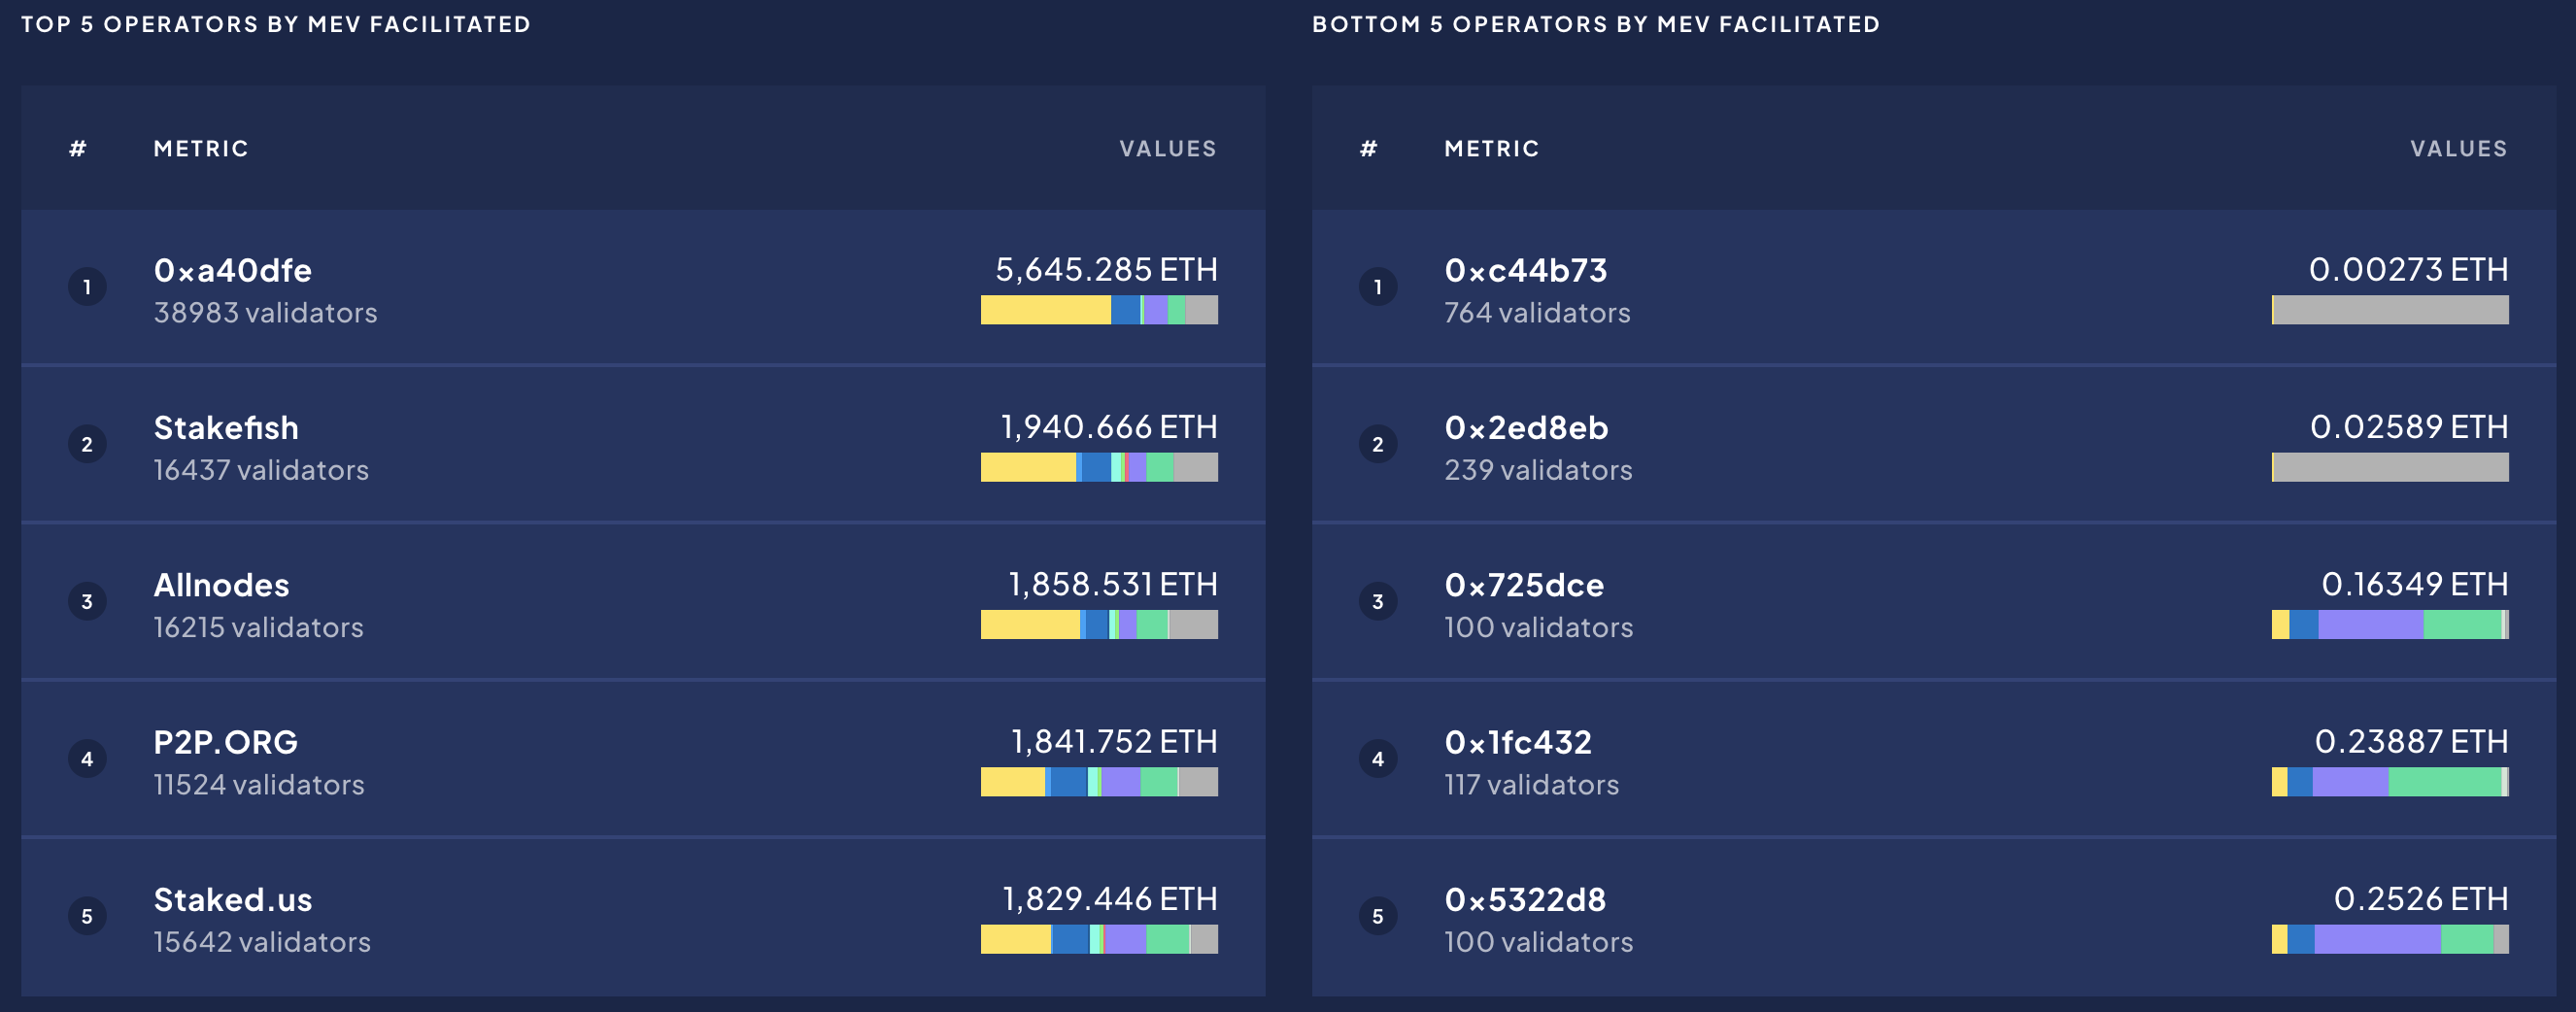
\includegraphics[width=\linewidth]{images/ratedtrend4}\\
(b)
\caption{Rated network explorer: top 5 and bottom 5 validators (a).  Top 5 and bottom 5 of operators that facilitated some MEV (total or average) (b), For both visualisations, select a timeframe: 1 day, 7 days, 30 days or all (since merge),1 June 2023}
\label{fig:ratedtrend4}
\end{center}
\end{figure}

\begin{figure}[htbp]
\begin{center}
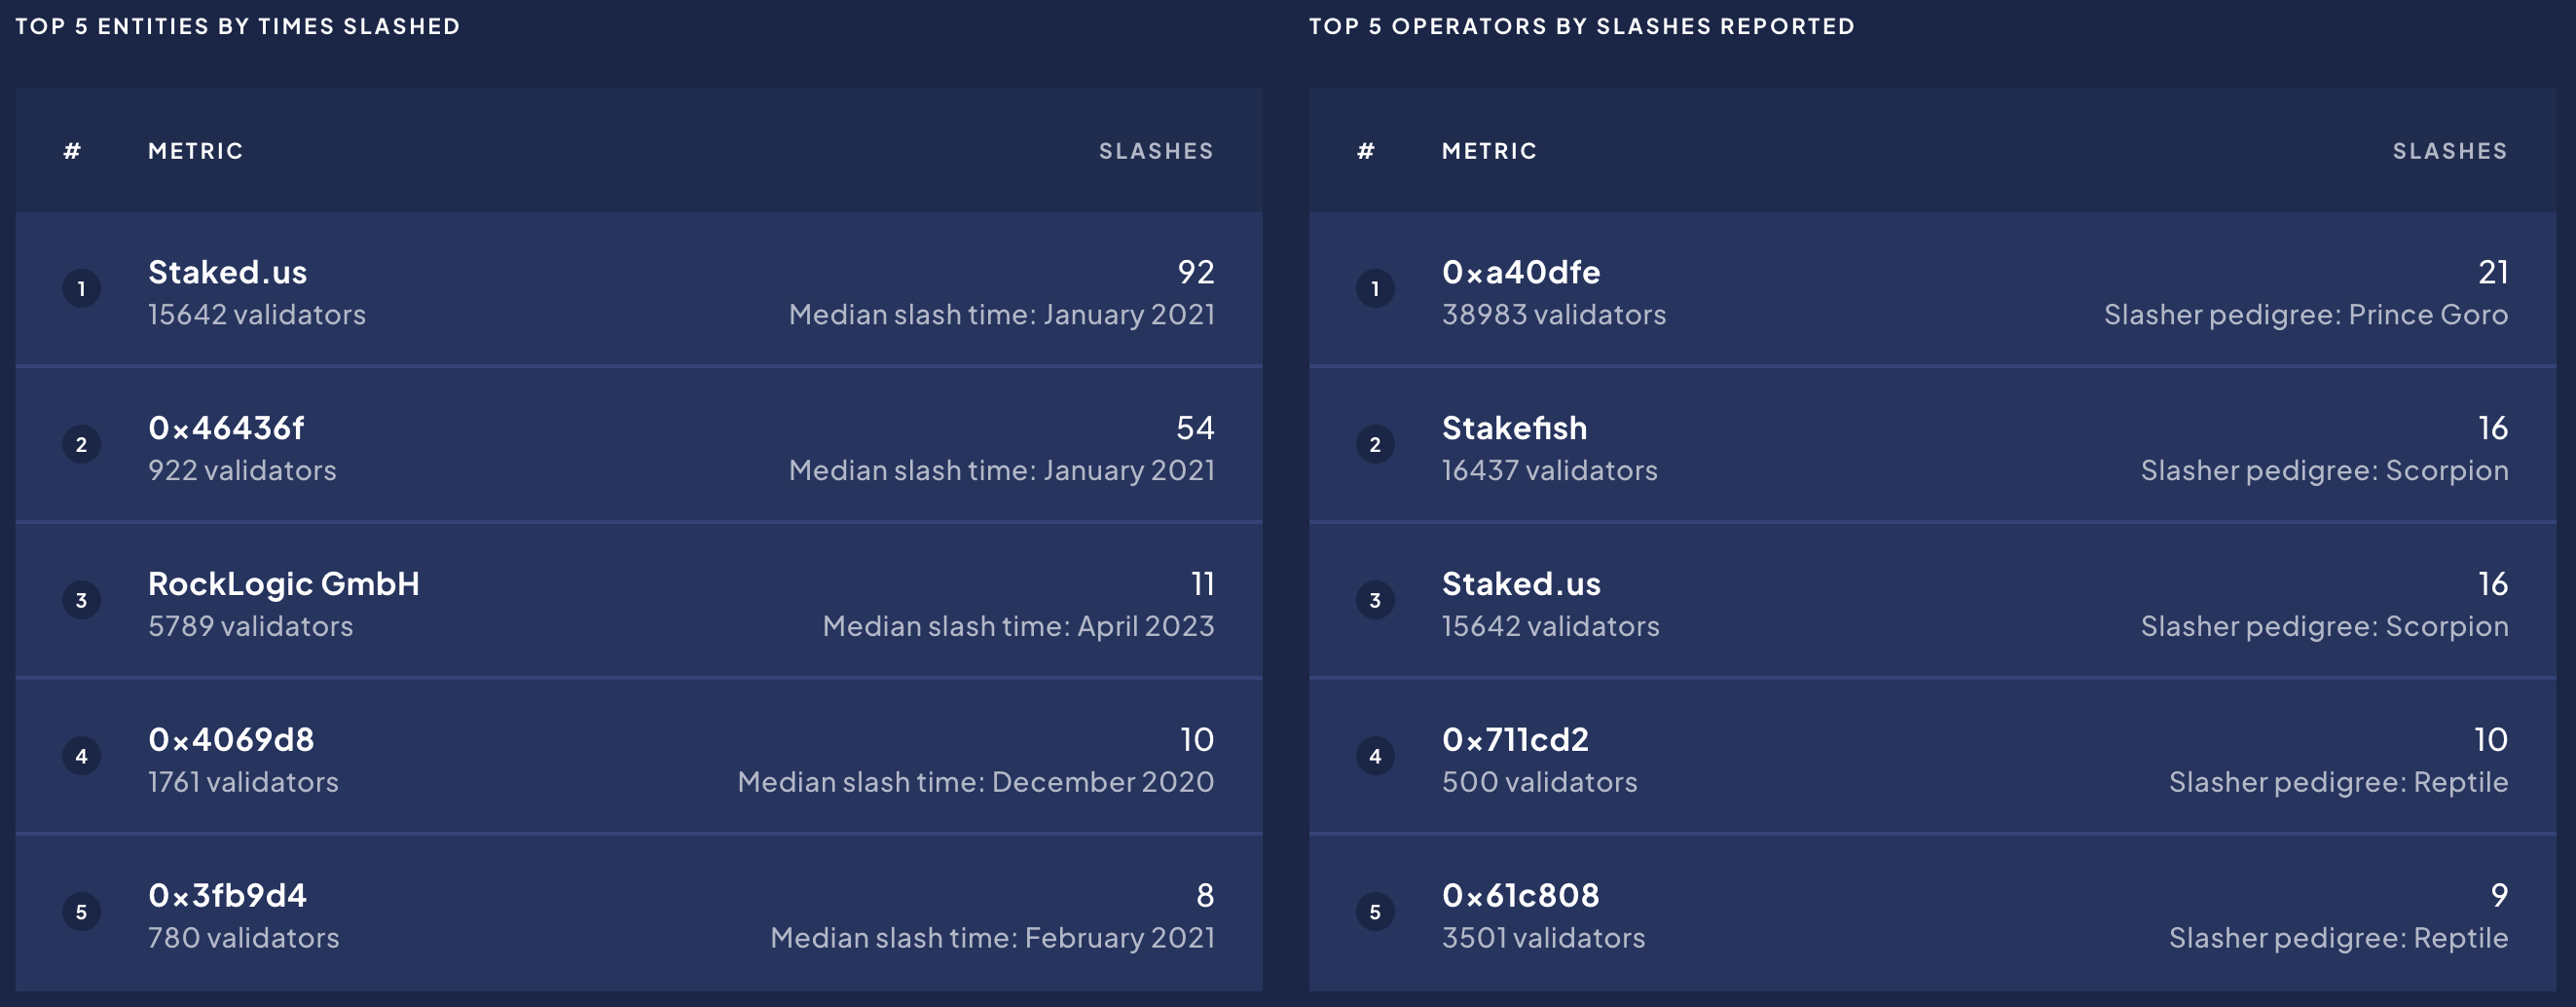
\includegraphics[width=\linewidth]{images/ratedtrend5}
\caption{Rated network explorer: top 5 entities by times slashed and top 5 operators by number of slashes reported. Select timeframes of 30 days, or all days (since merge) , 1 June 2023}
\label{fig:ratedtrend5}
\end{center}
\end{figure}

\begin{figure}[htbp]
\begin{center}
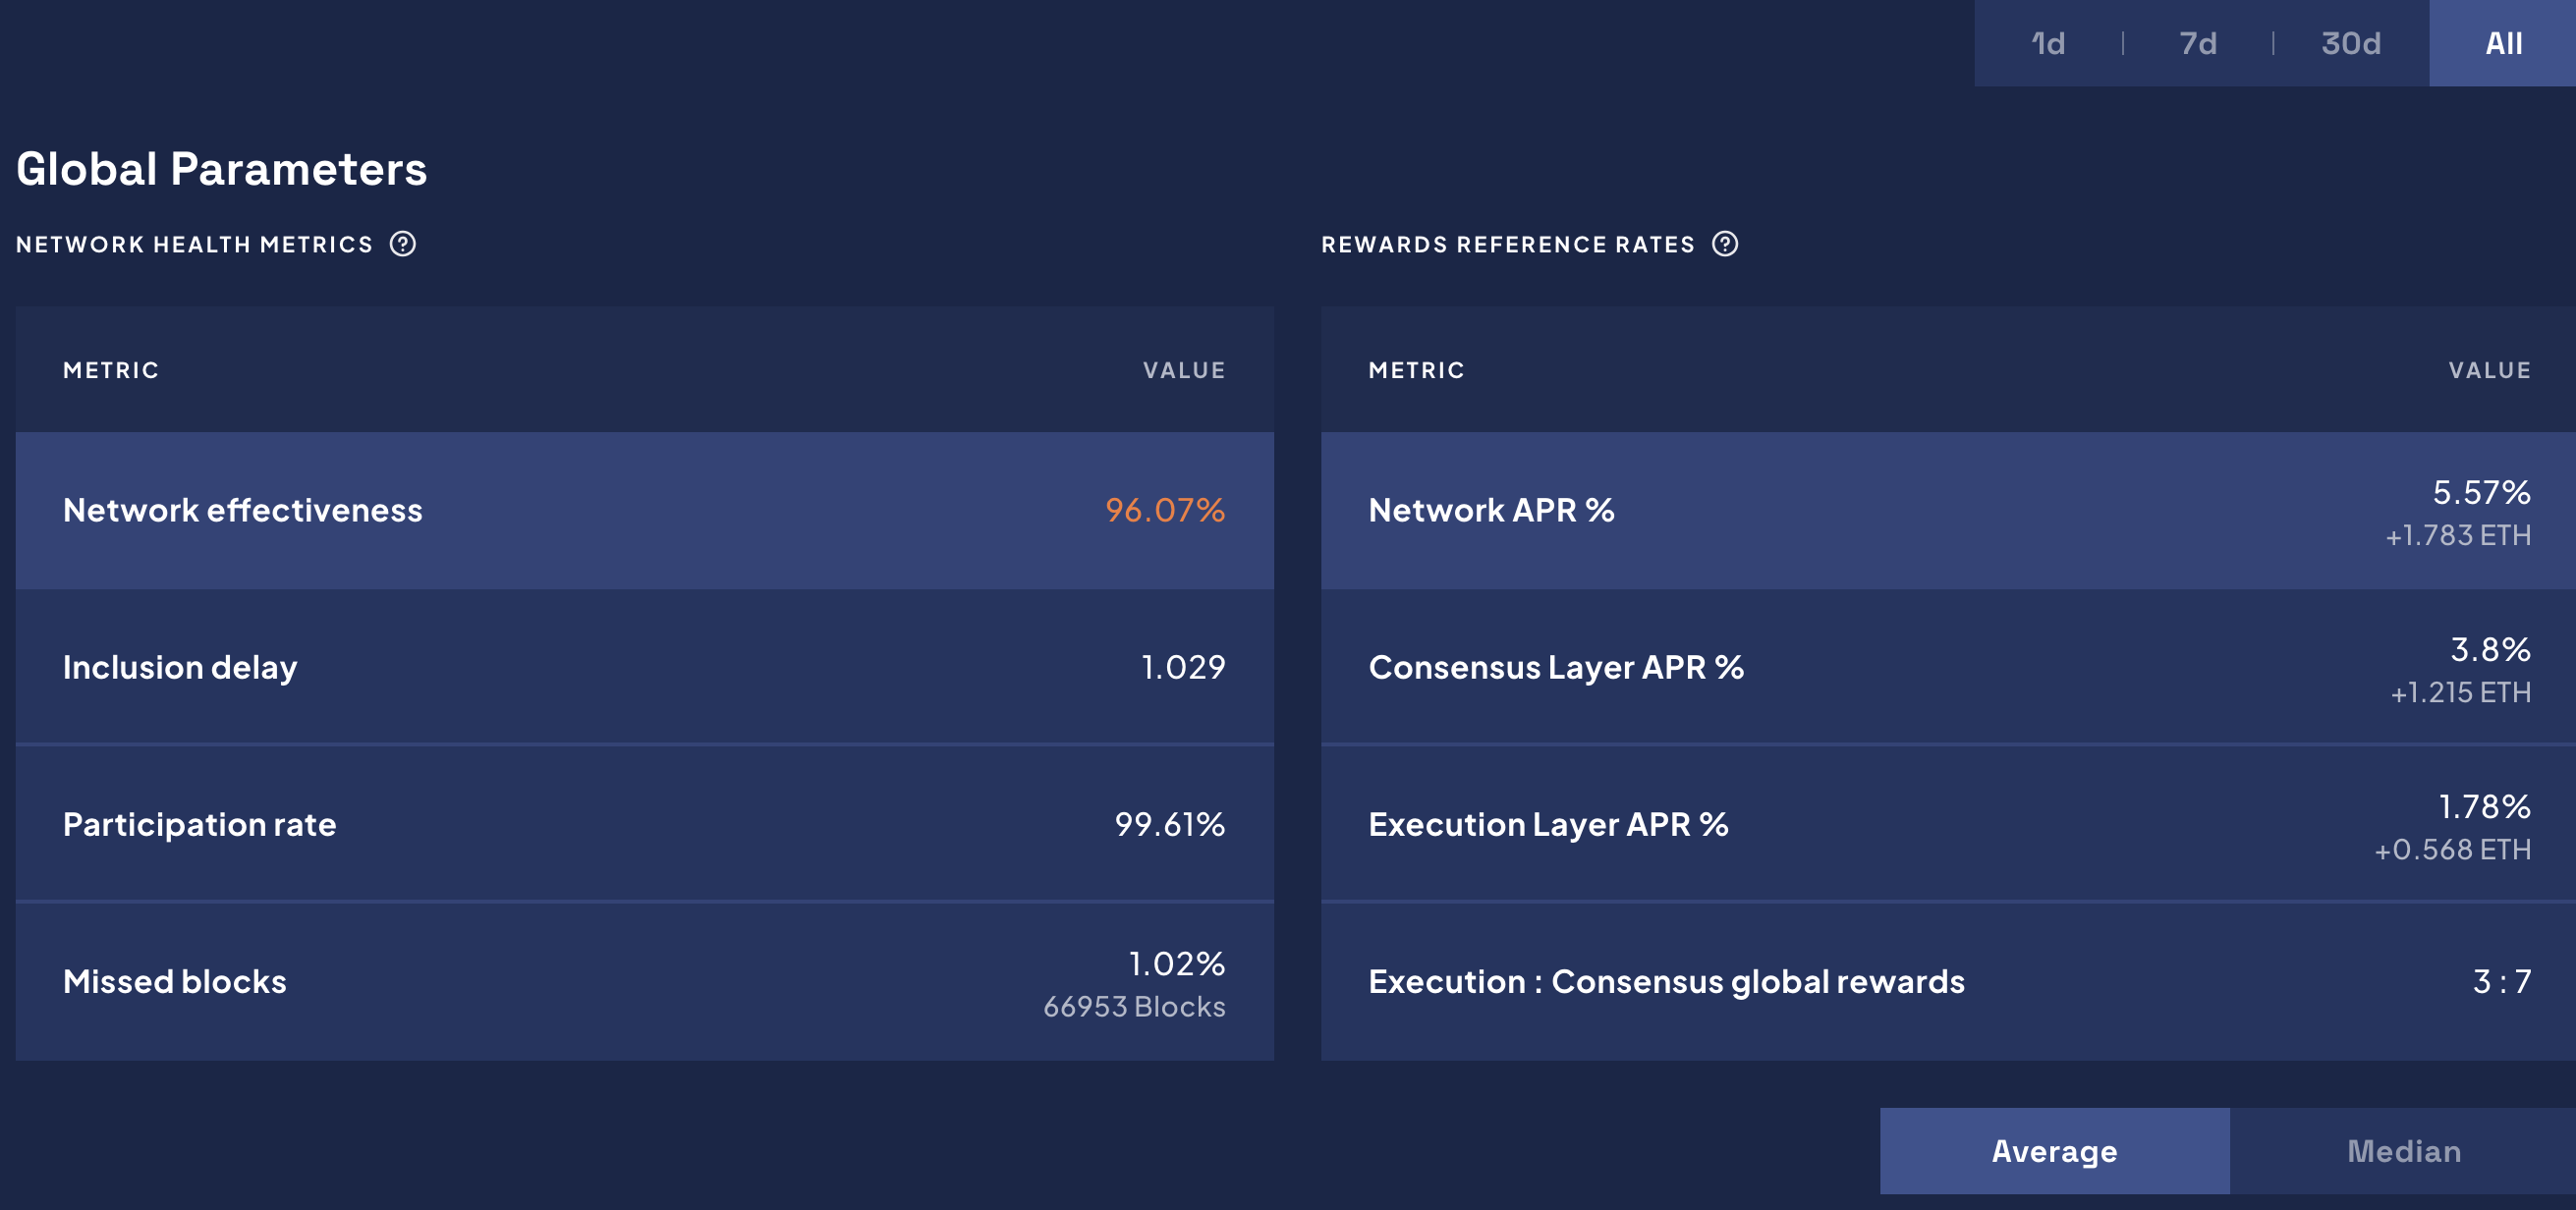
\includegraphics[width=\linewidth]{images/ratednw1}\\
(a)
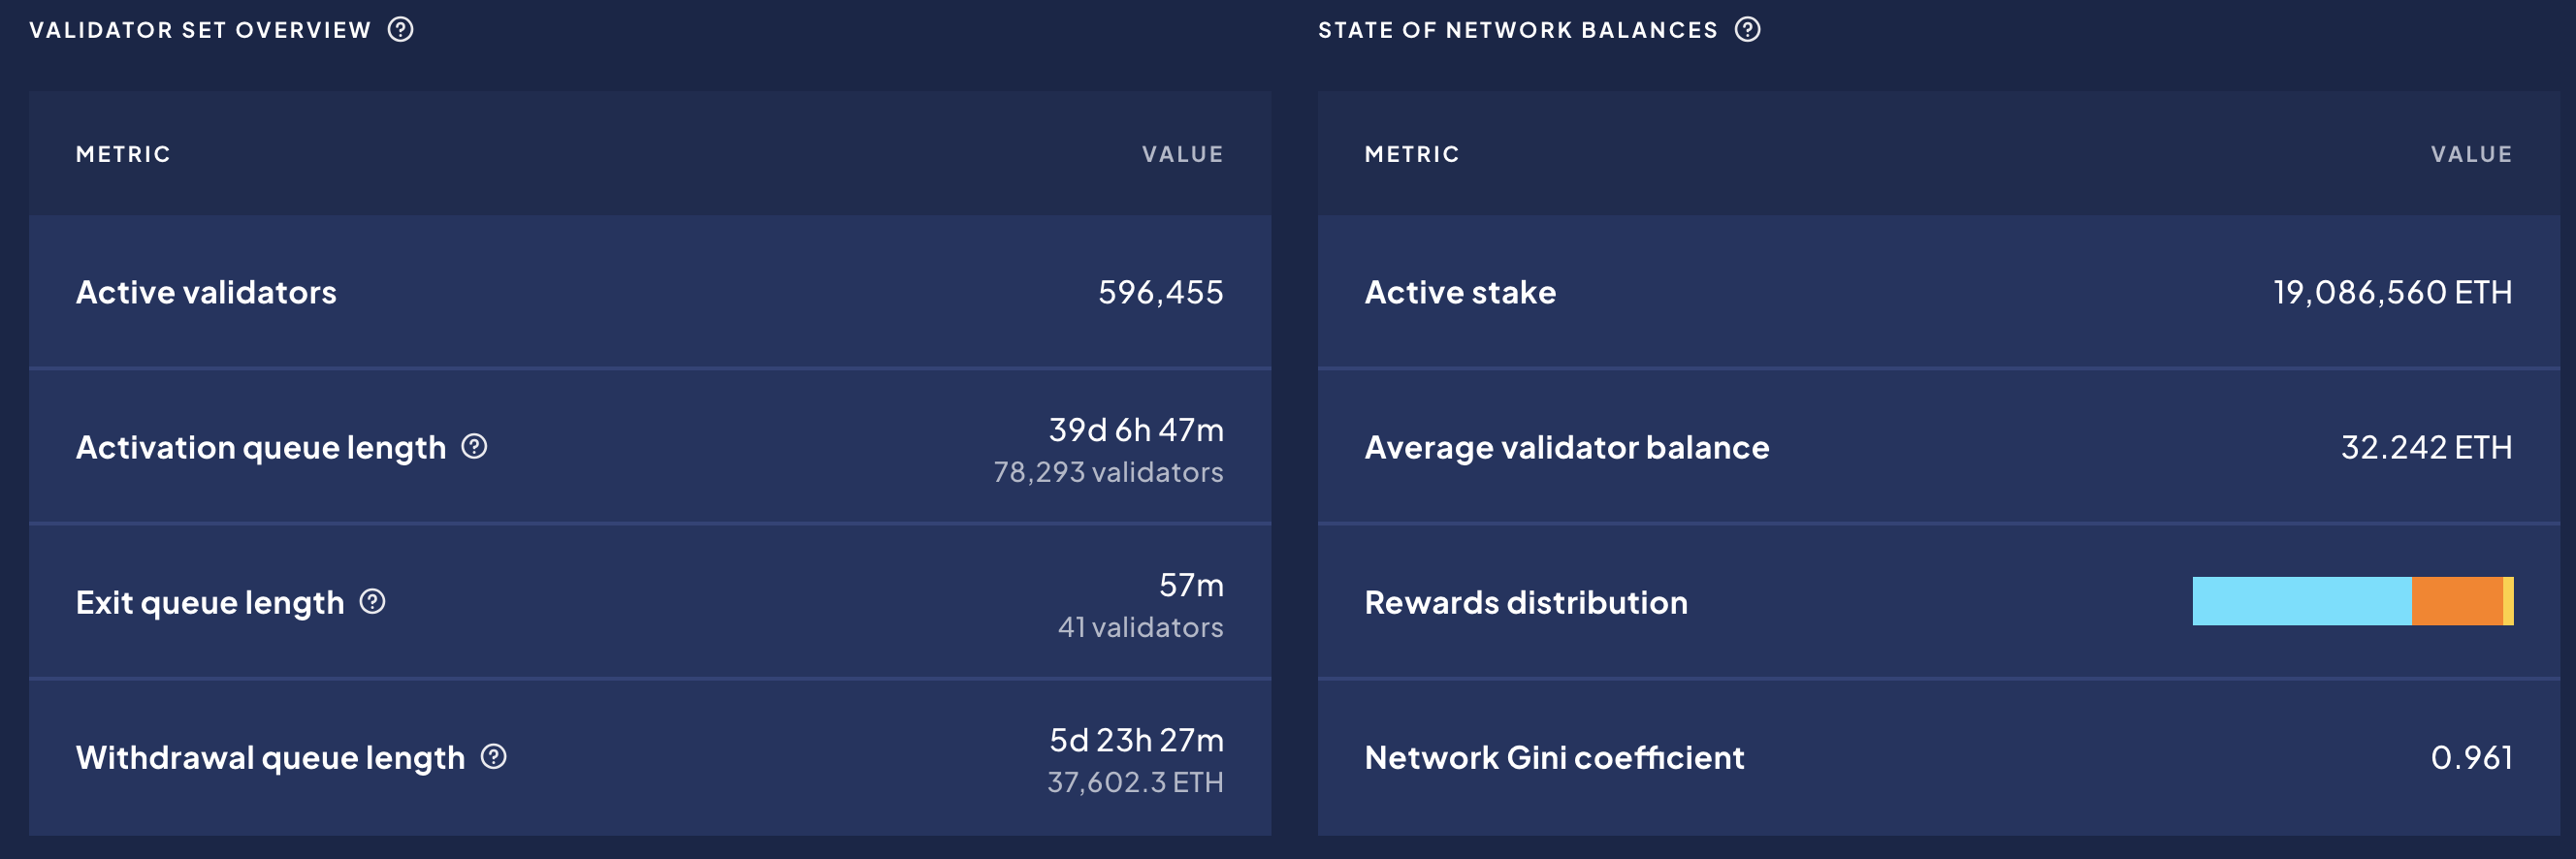
\includegraphics[width=\linewidth]{images/ratednw2}\\
(b)
\caption{Rated network explorer: high level metrics to reflect the health of the network  (a) and four reference rates of return for the entire active validator set. (b), For both visualisations, select a timeframe: 1 day, 7 days, 30 days or all (since merge),1 June 2023}
\label{fig:ratednw1}
\end{center}
\end{figure}

\begin{figure}[htbp]
\begin{center}
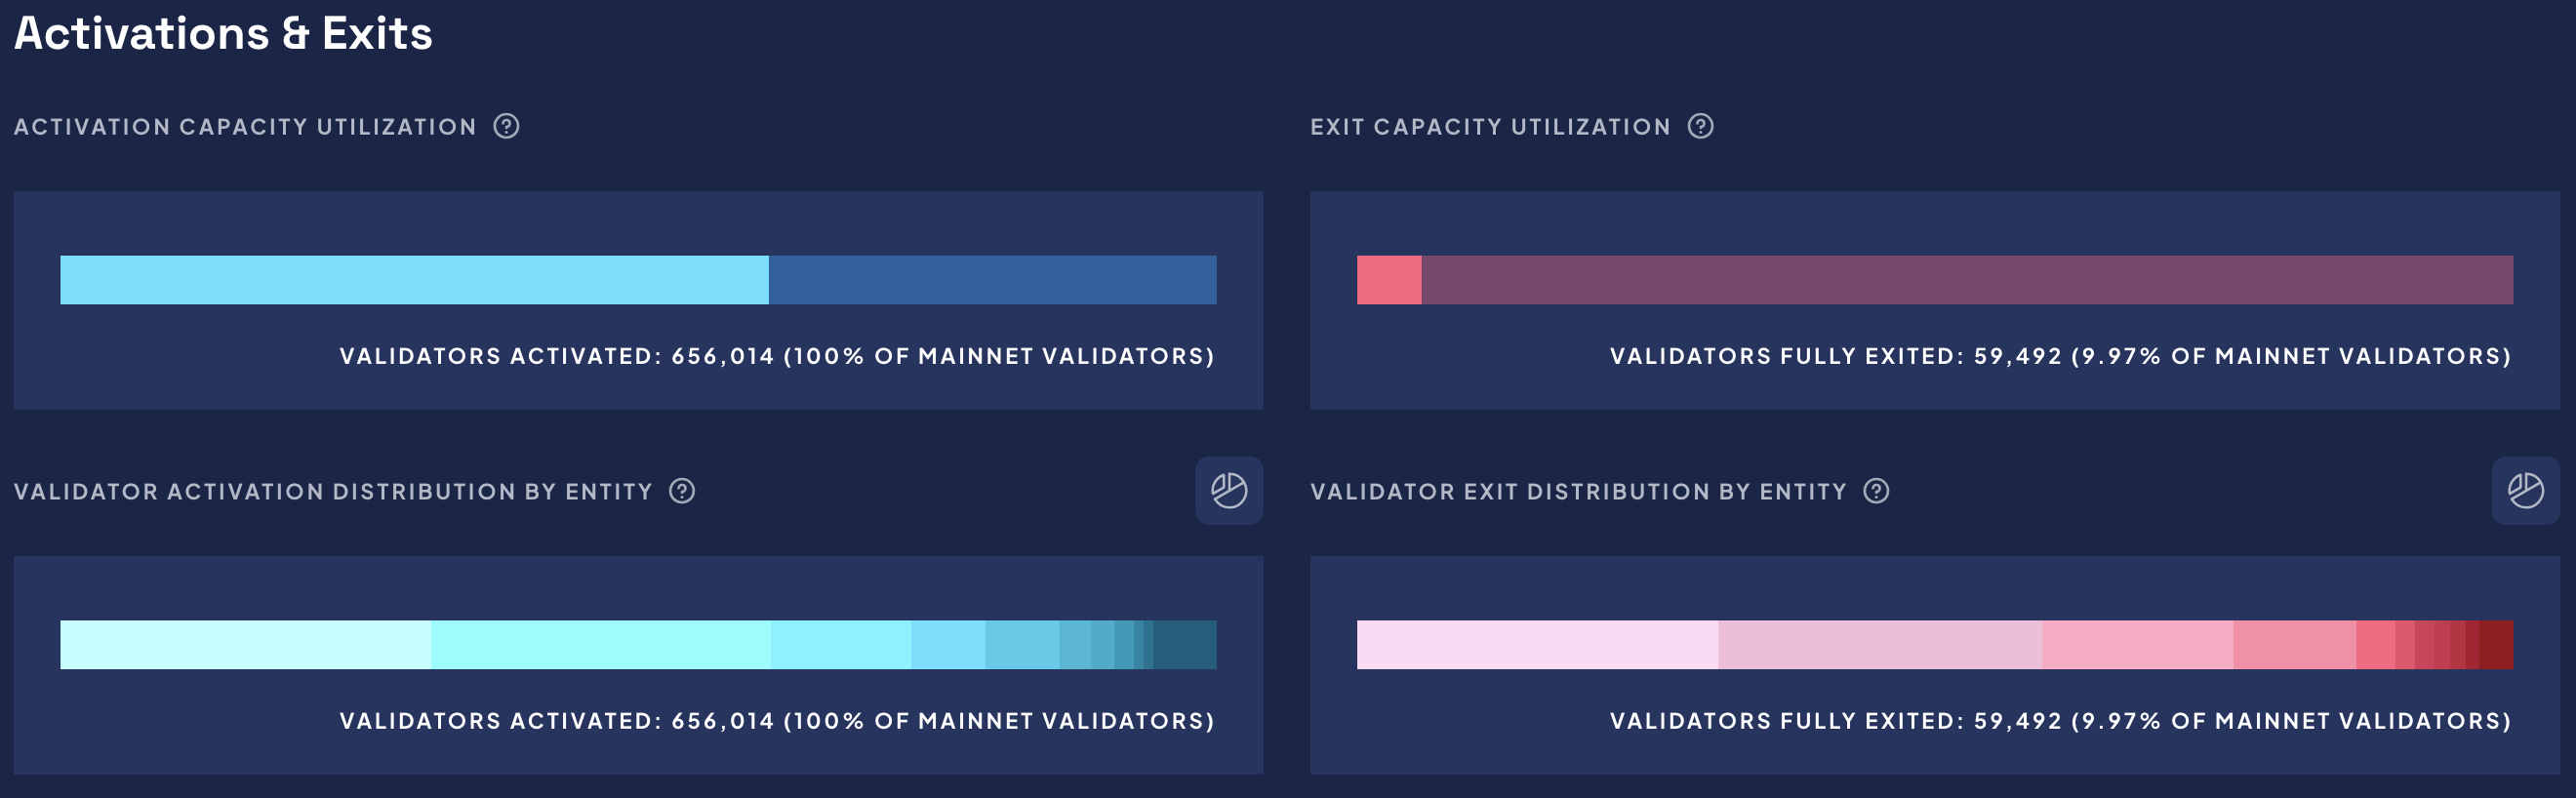
\includegraphics[width=\linewidth]{images/ratednw3}\\
(a)
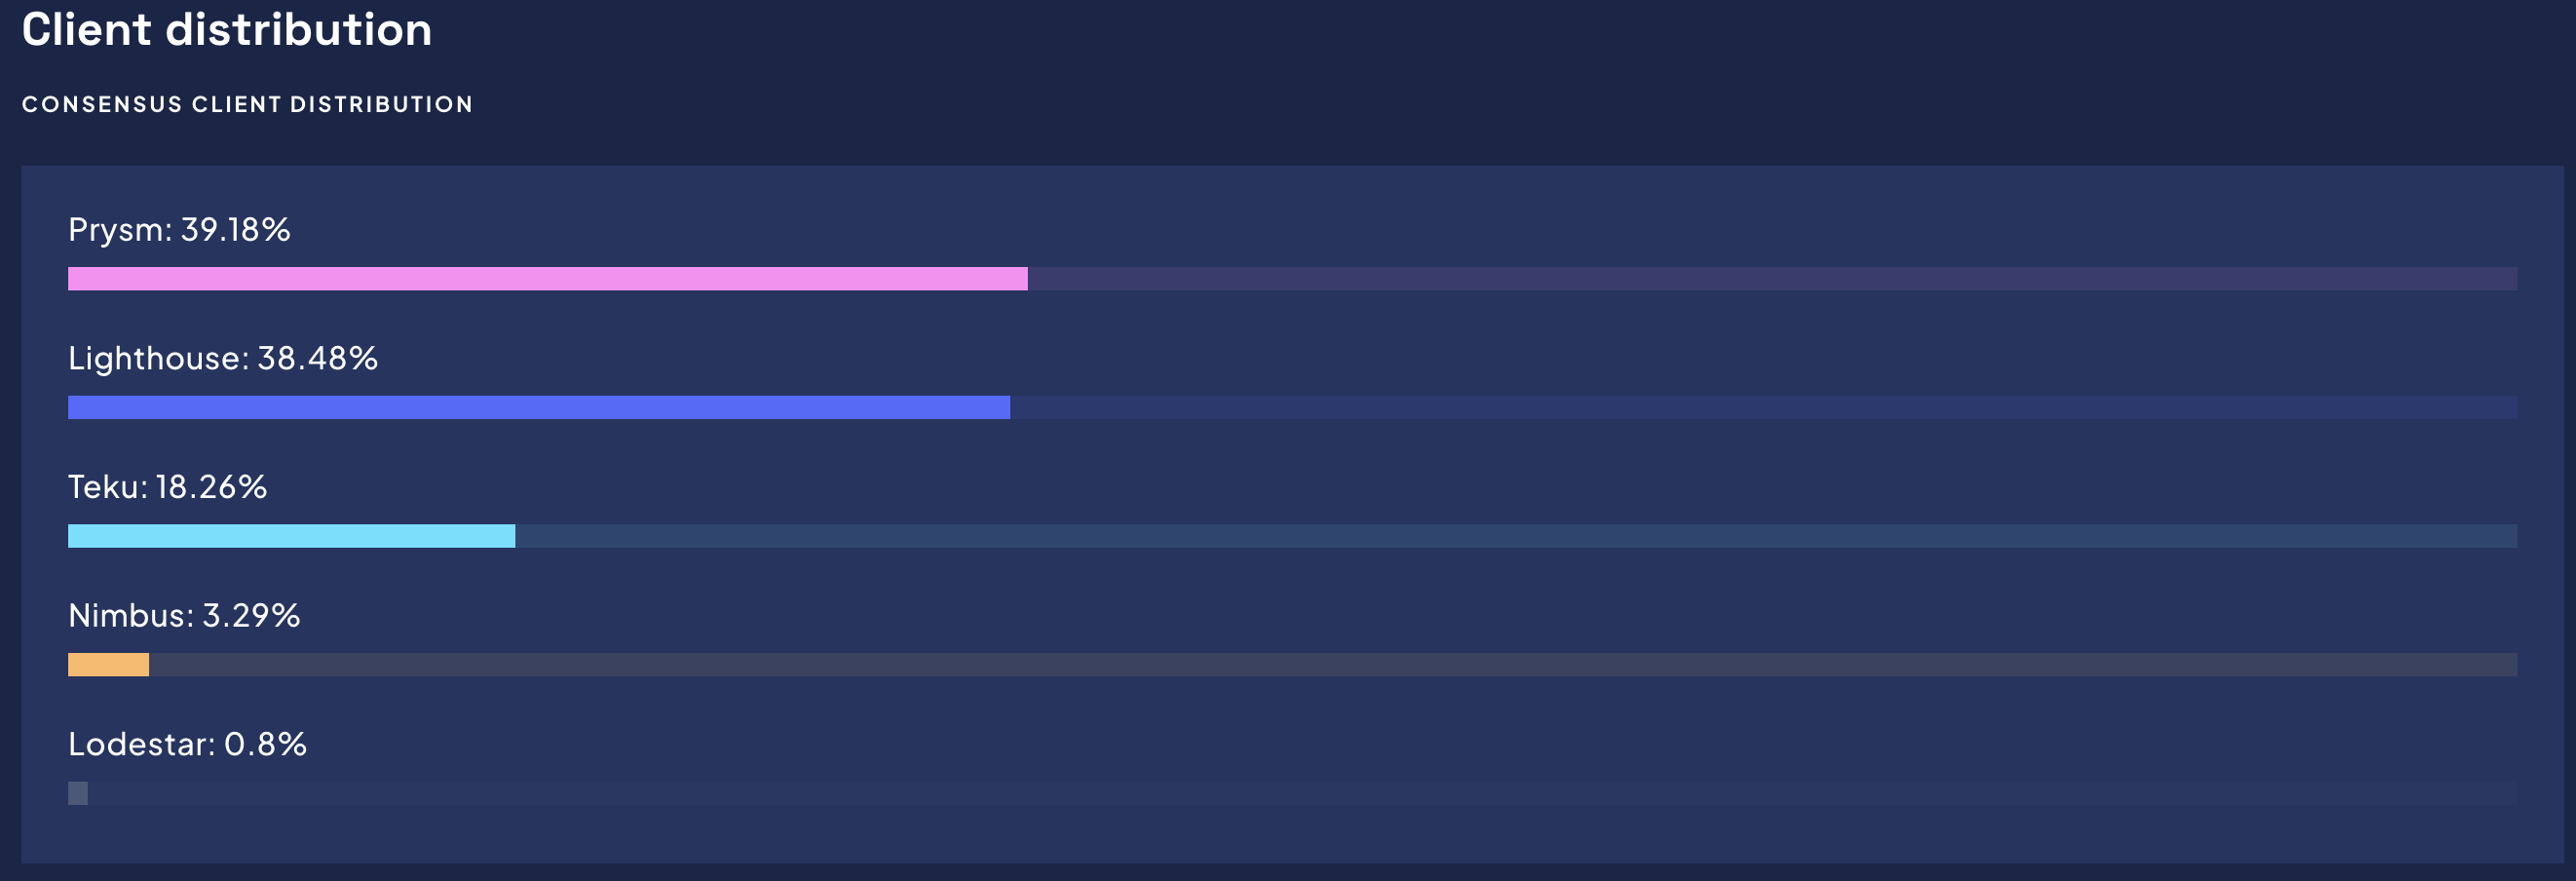
\includegraphics[width=\linewidth]{images/ratednw4}\\
(b)
\caption{Rated network explorer: activation \& exits information: the number of validators activated and the proportion of activation capacity for selected timeframe, and similarly for validators exiting.  (a) and four reference rates of return for the entire active validator set. (b), For both visualisations, select a timeframe: 1 day, 7 days, 30 days or all (since merge),1 June 2023}
\label{fig:ratednw4}
\end{center}
\end{figure}

\clearpage
\textbf{MEV Relay Landscape}\\
% ---------------------------------------
\begin{figure}[htbp]
\begin{center}
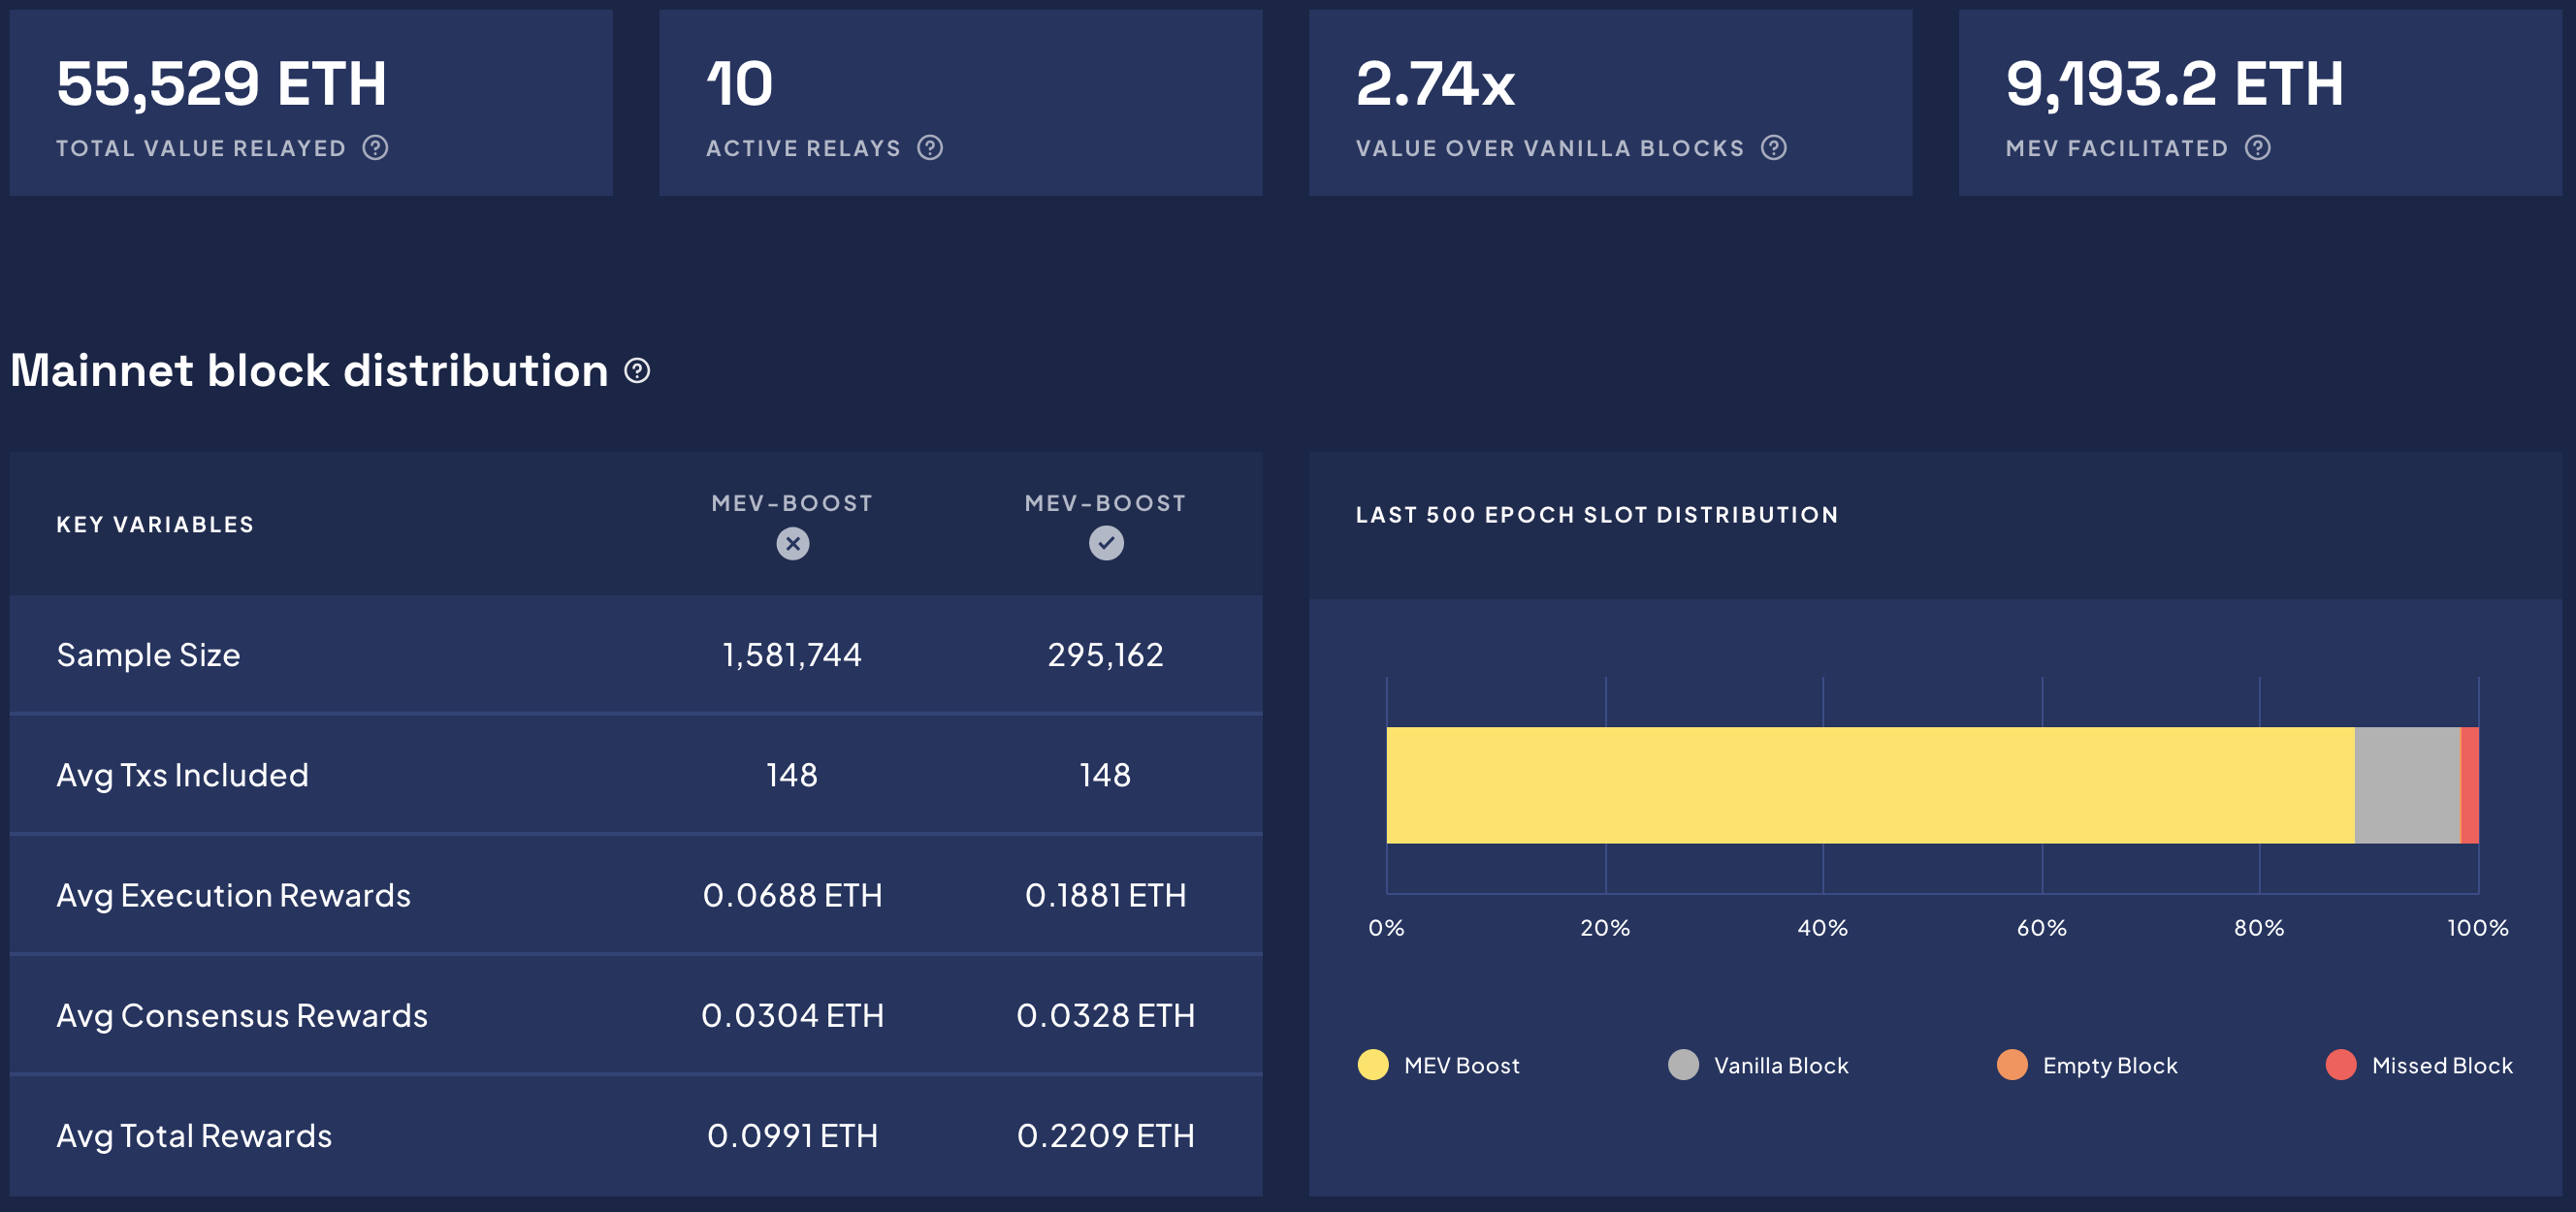
\includegraphics[width=\linewidth]{images/ratedrelay1}
\caption{Rated network explorer: MEV relay summary statistics for 30 days, selected from timeframes: 1 day, 7 days, 30 days or all (since merge), 6 June 2023}
\label{fig:ratedrelay1}
\end{center}
\end{figure}

\begin{figure}[htbp]
\begin{center}
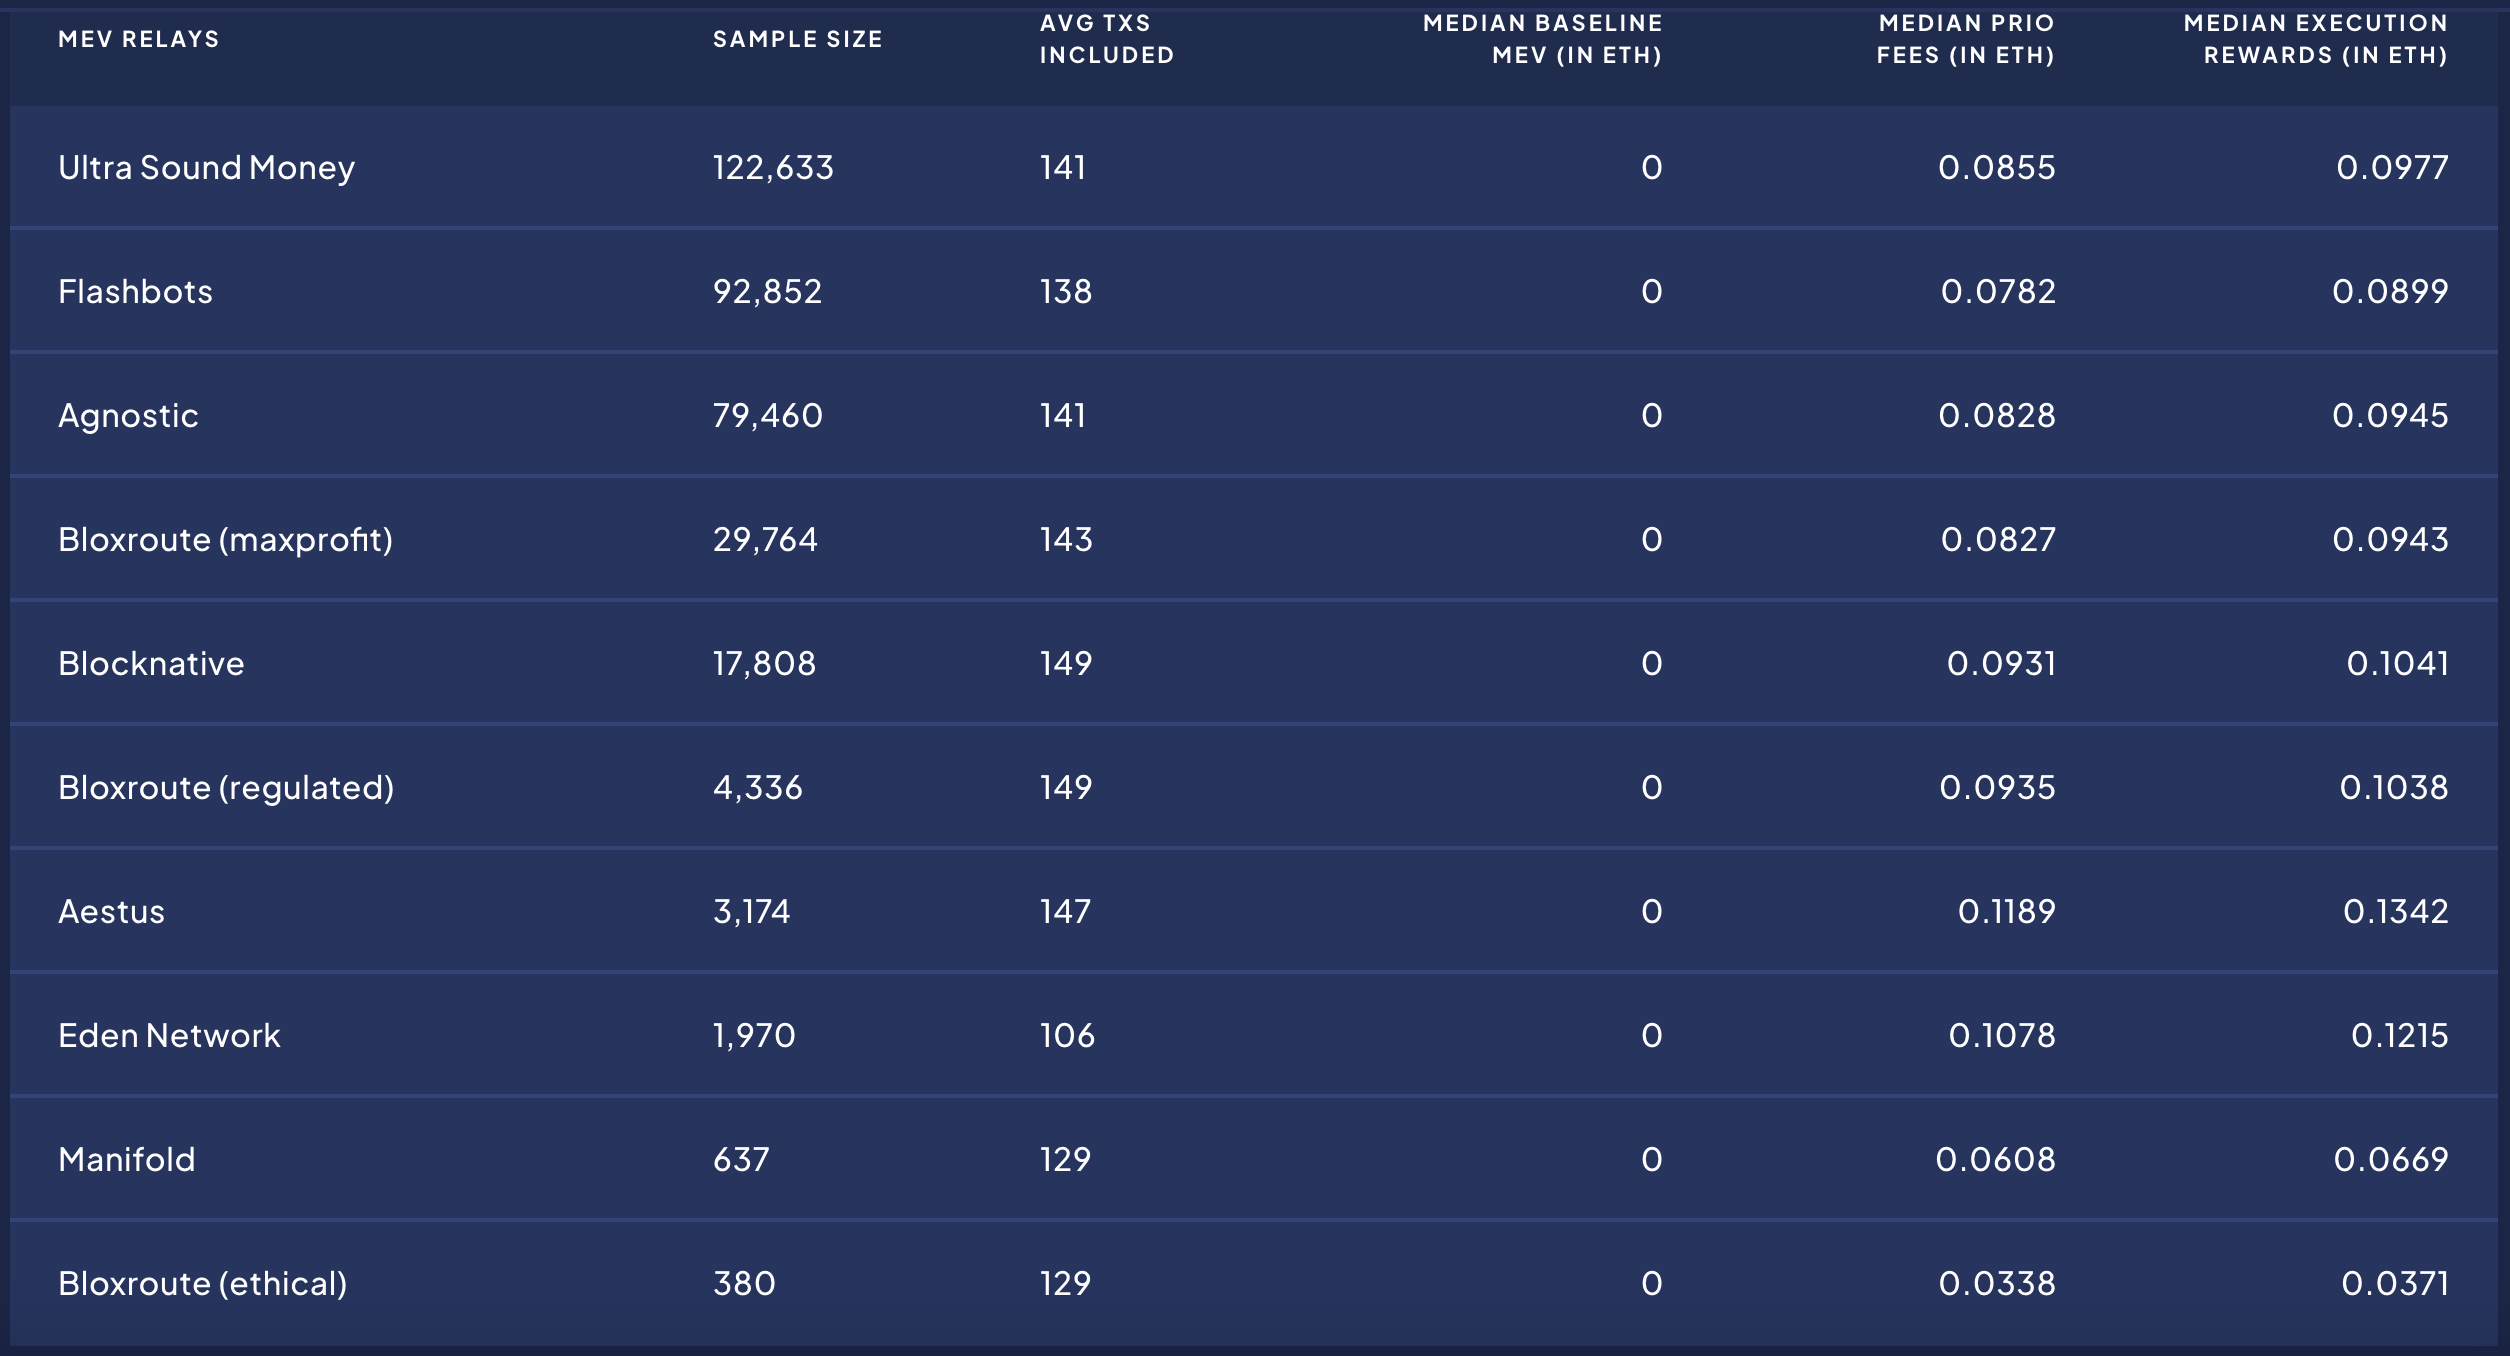
\includegraphics[width=\linewidth]{images/ratedrelay2}
\caption{Rated network explorer: Comparison between MEV relays for blocks procured from relays that were included in the canonical chain for all days, selected from timeframes: 1 day, 7 days, 30 days or all (since merge), 6 June 2023}
\label{fig:ratedrelay2}
\end{center}
\end{figure}

\begin{figure}[htbp]
\begin{center}
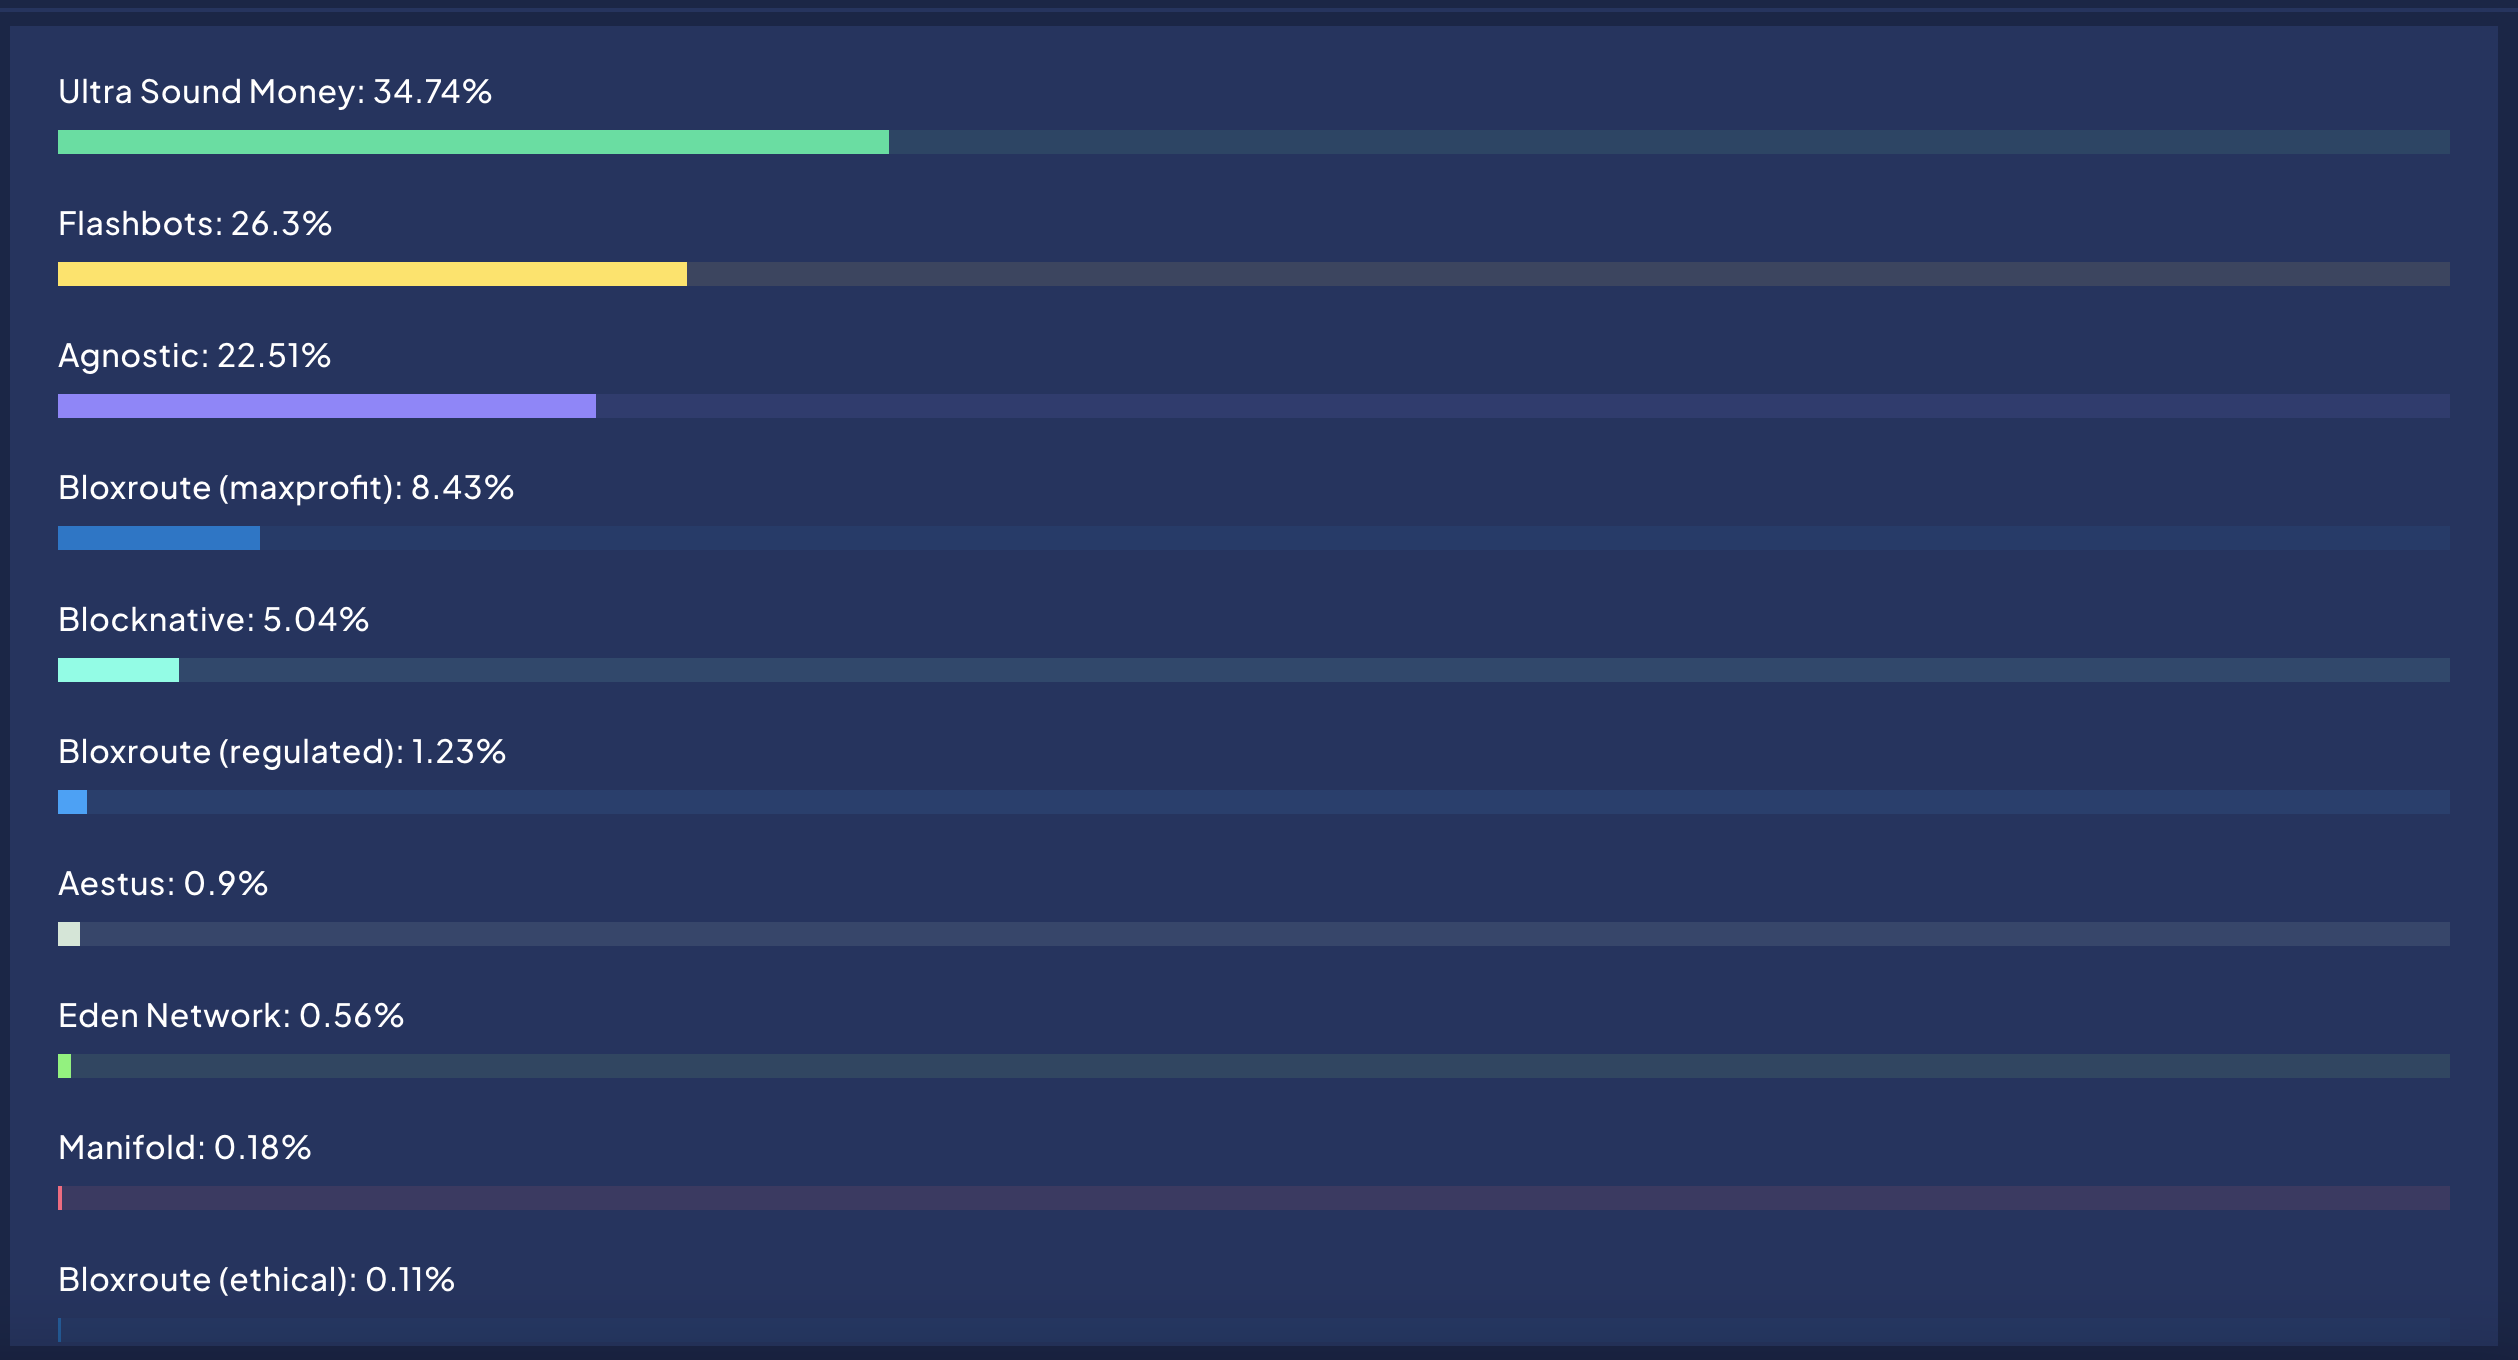
\includegraphics[width=\linewidth]{images/ratedrelay3}
\caption{Rated network explorer: MEV-boost relay market share selecting all days from timeframes: 1 day, 7 days, 30 days or all (since merge), 6 June 2023}
\label{fig:ratedrelay3}
\end{center}
\end{figure}

\clearpage
\textbf{MEV Builder Landscape}
% ---------------------------------------
\begin{figure}[htbp]
\begin{center}
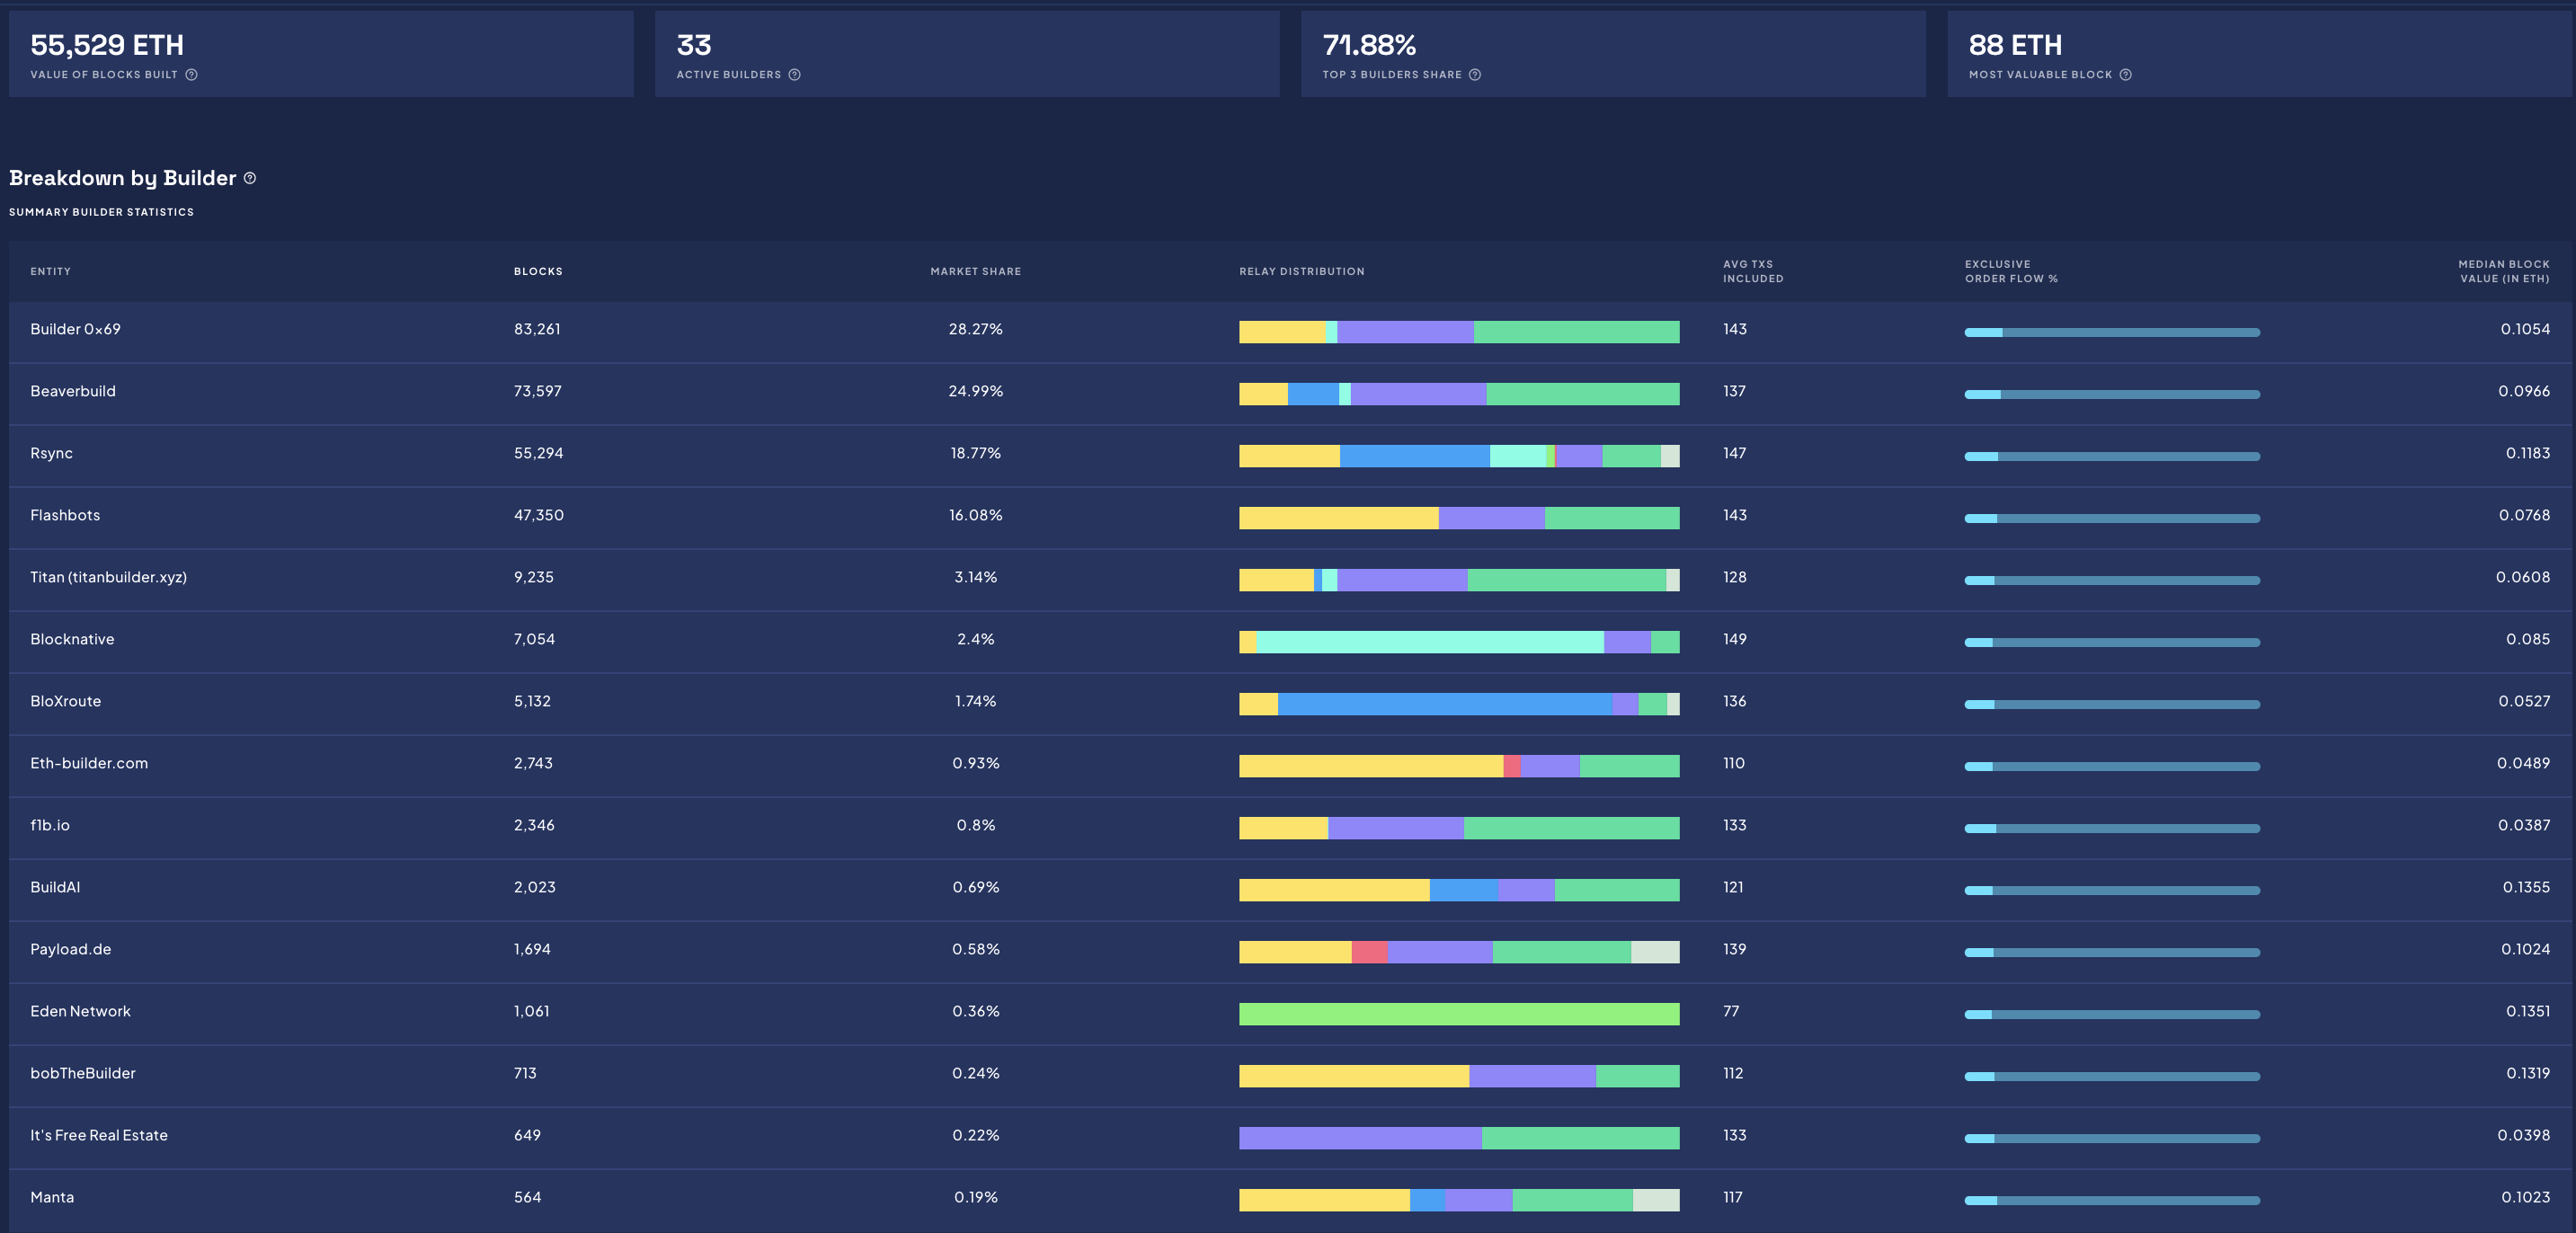
\includegraphics[width=\linewidth]{images/ratedbuilder}
\caption{Rated network explorer: MEV relay summary statistics for 30 days, selected from timeframes: 1 day, 7 days, 30 days or all (since merge), 6 June 2023}
\label{fig:ratedbuilder}
\end{center}
\end{figure}

\textbf{Diversified Staked ETH Index (dsETH) from Index Coop}
% ---------------------------------------
\begin{figure}[htbp]
\begin{center}
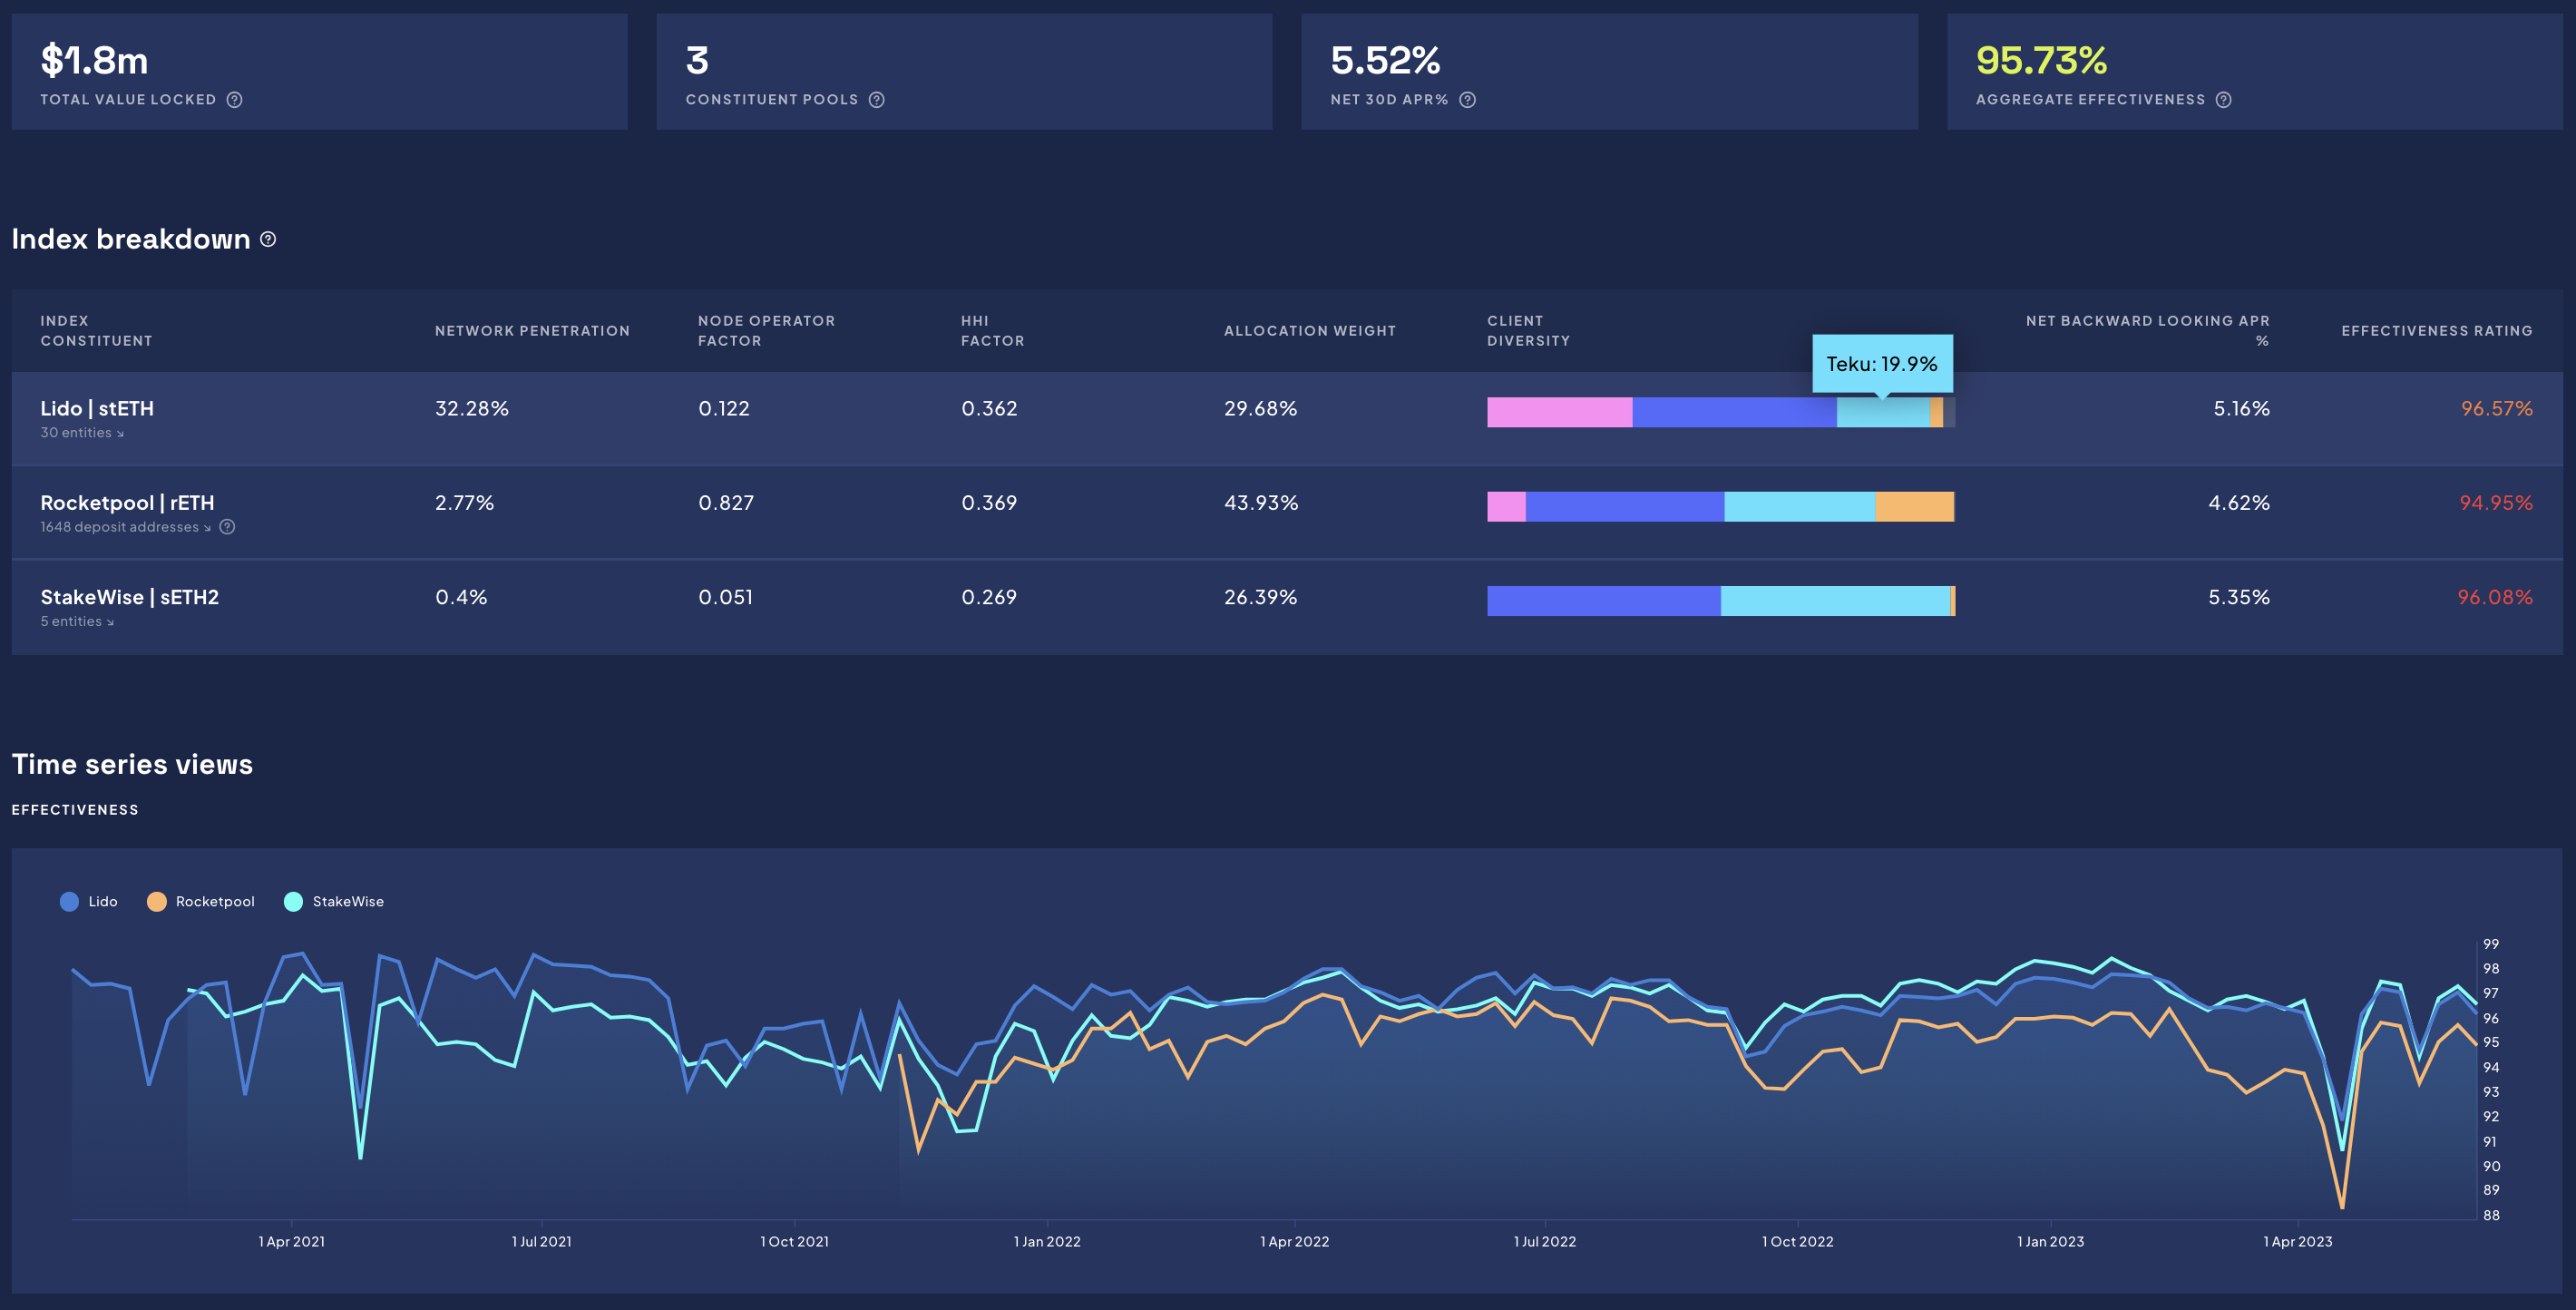
\includegraphics[width=0.9\linewidth]{images/ratedcoop}
\caption{Rated network explorer: Key metrics of staked ETH index and time series for all available days, selected from timeframes: 1 day, 7 days, 30 days or all (since merge), 6 June 2023}
\label{fig:ratedcoop}
\end{center}
\end{figure}


\clearpage
% --------------------------------------
\subsubsection*{Etherscan}
% --------------------------------------
There are several webpages with detailed information on transactions, blocks, accounts and tokens. In the screenshots below, figures~\ref{fig:txns}-~\ref{fig:erc20} on pages~\pageref{fig:txns}-~\pageref{fig:erc20}), are a few extracts from the detailed information on Etherscan and the data visualisations provided by them. Many of the dashboards allow the user to interact with the data being displayed by entering specific validators, blocks etc, that are of interest, or selecting one of the different time periods available. 

Moreover, there are several summary graphs and visualisations that have been created and are displayed in the \textit{Charts \& Statistics} section of the website. These visualisations are shown in figures~\ref{fig:ethdaily}-~\ref{fig:dailyverified} on pages~\pageref{fig:ethdaily}~-~\pageref{fig:dailyverified}. There is some degree of interactivity in these charts and diagrams, which includes the ability to zoom in on a section of a graph in several instances.\\

\begin{figure}[htbp]
\begin{center}
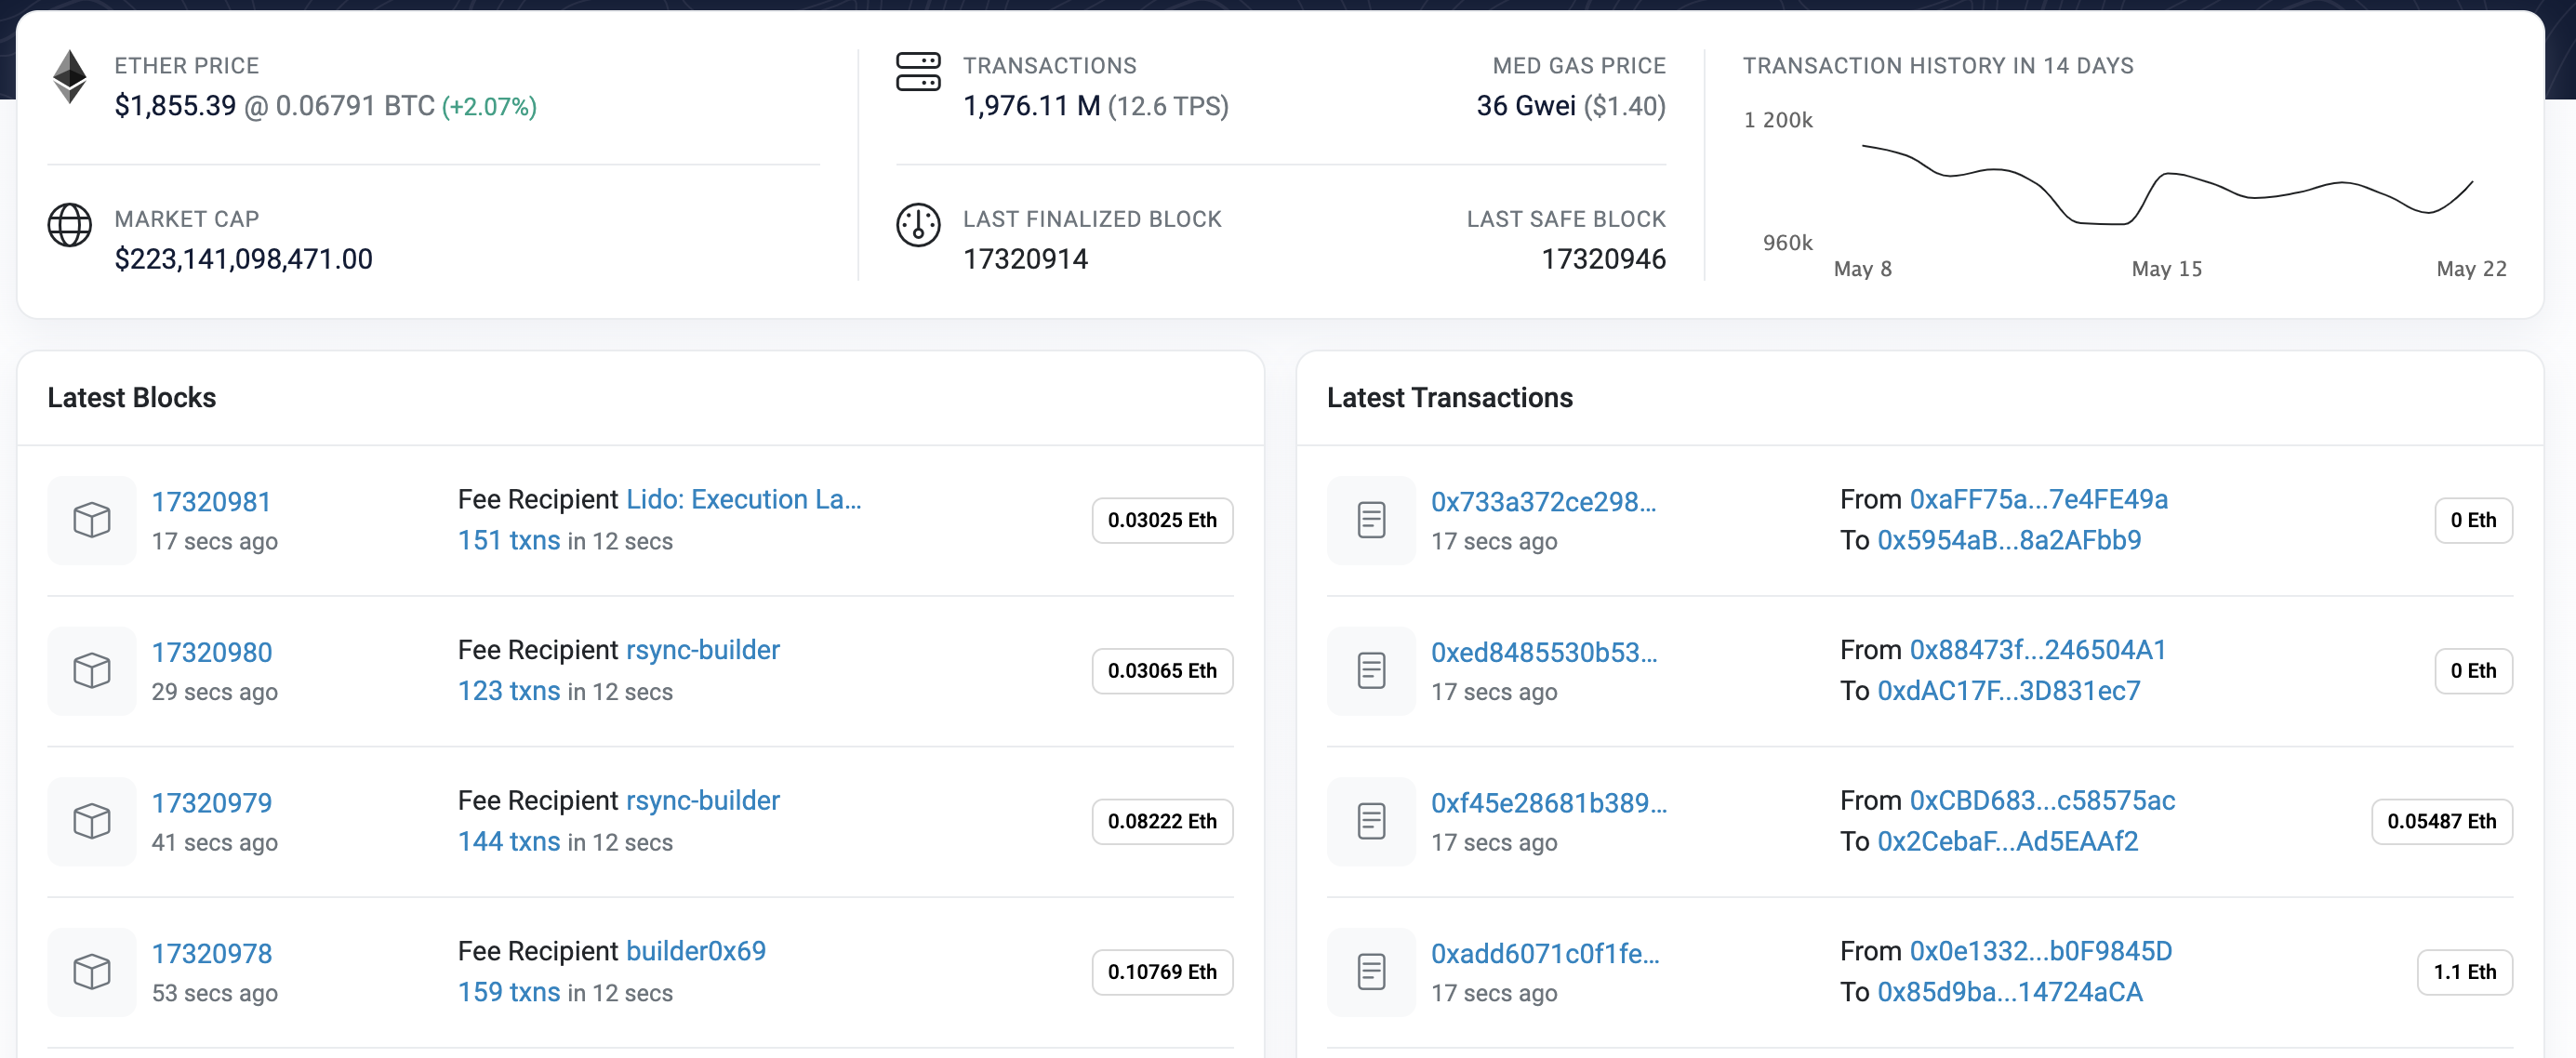
\includegraphics[width=\linewidth]{images/etherscan}
\caption{Etherscan home page, 23 May 2023}
\label{fig:ethscan}
\end{center}
\end{figure}


\textbf{Detailed blockchain data}\\
% ------------------------------------------
\begin{figure}[htbp]
\begin{center}
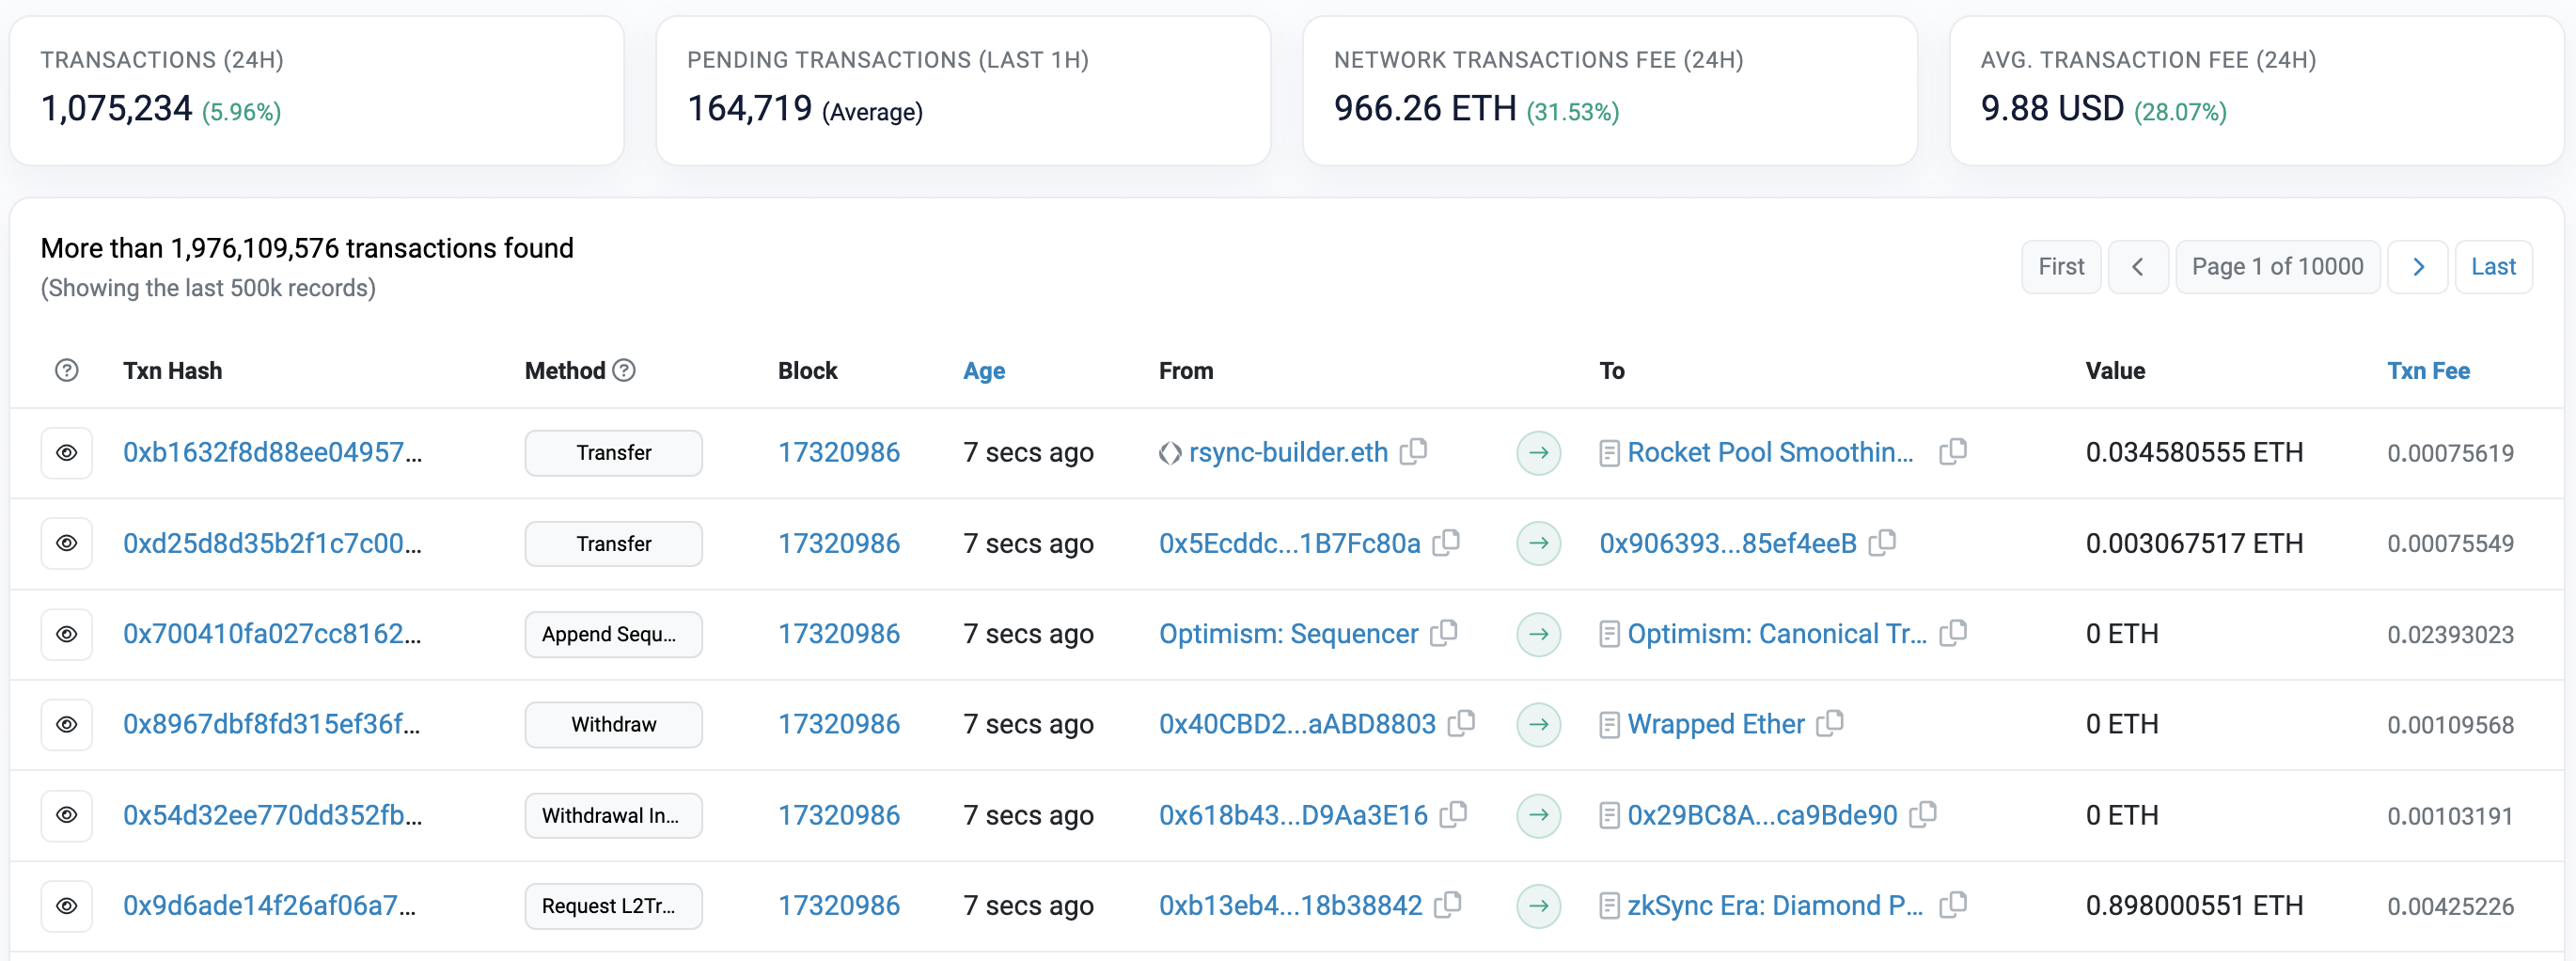
\includegraphics[width=0.48\linewidth]{images/txns}
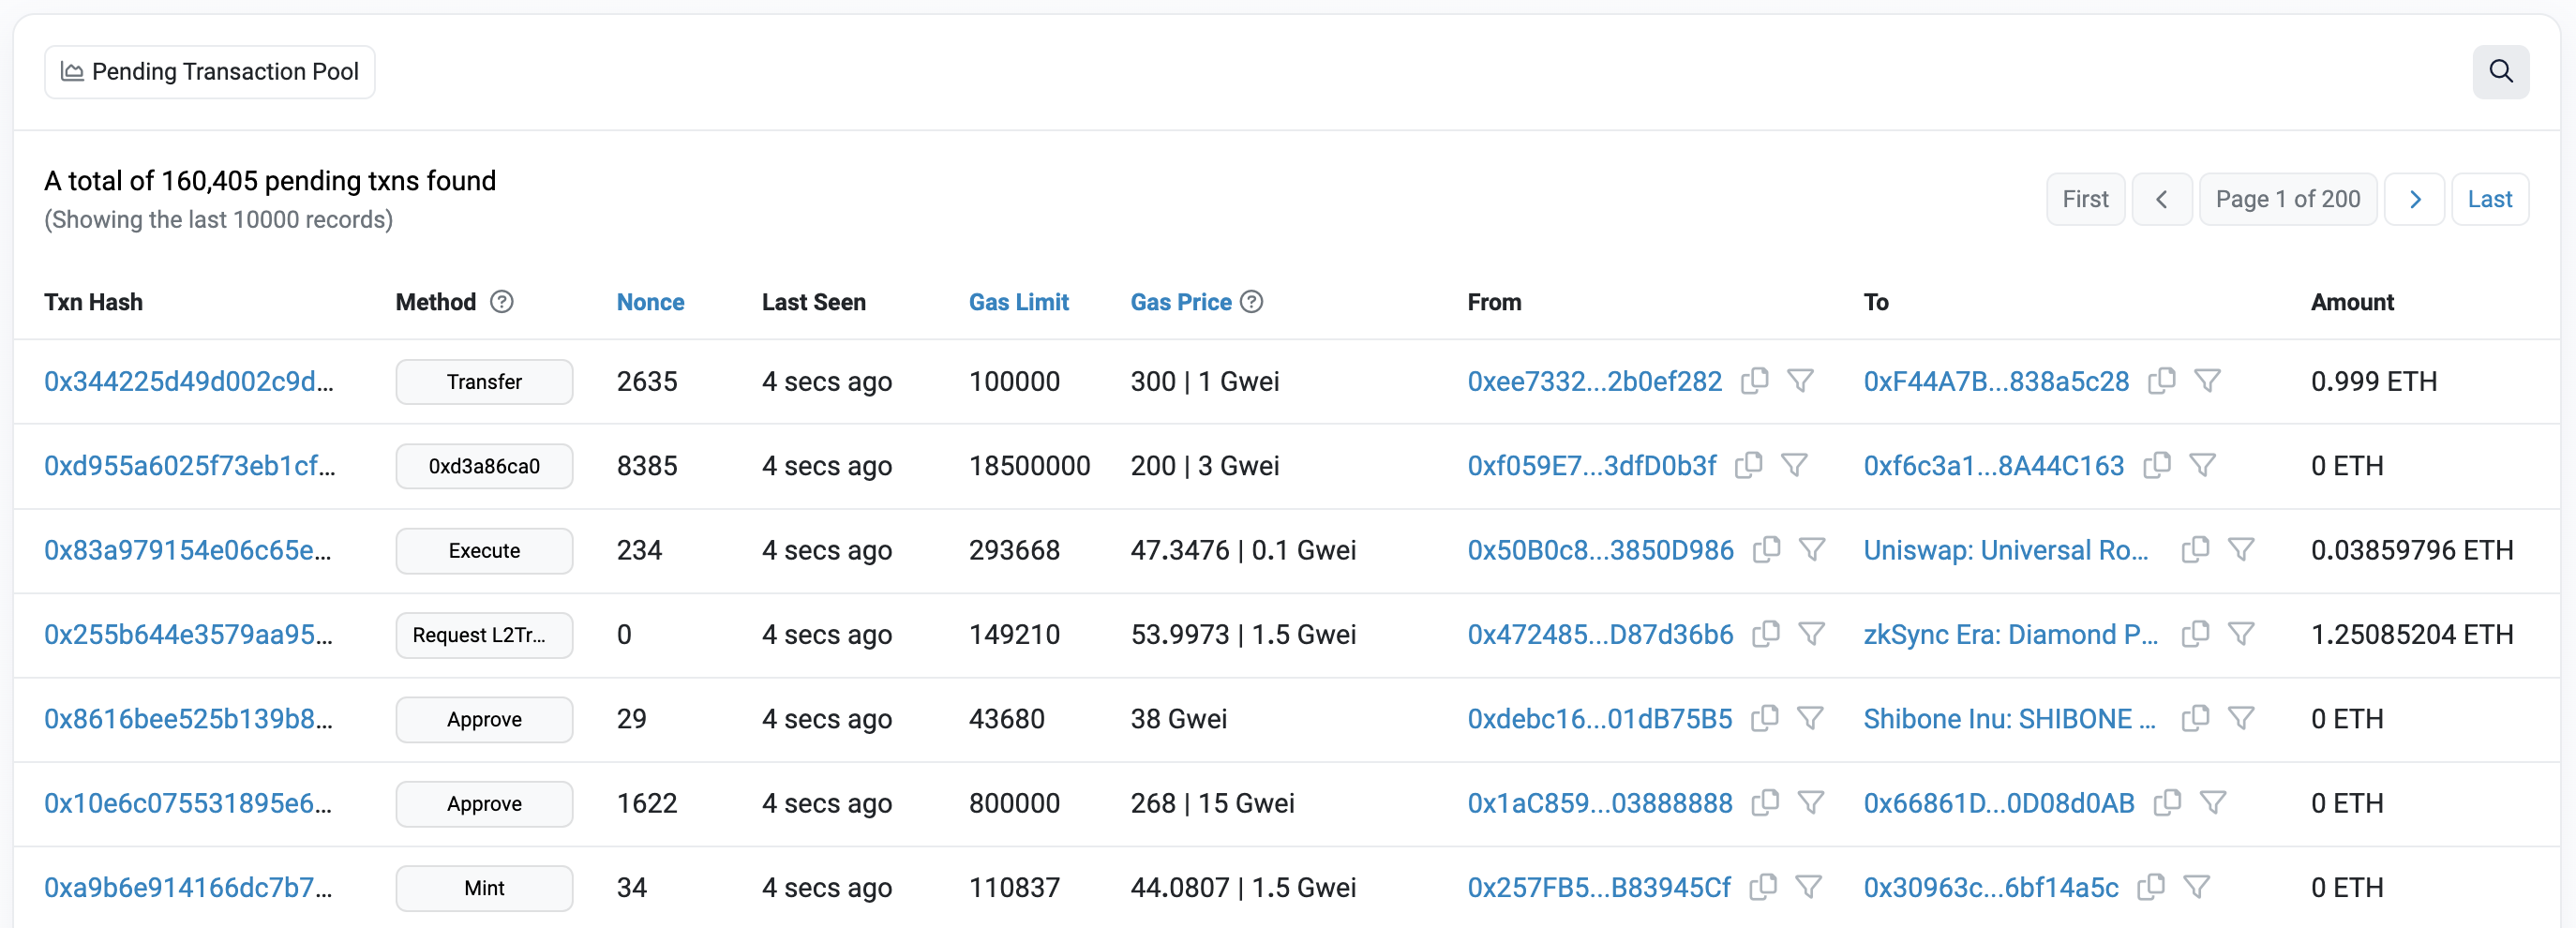
\includegraphics[width=0.48\linewidth]{images/pendtxns} \\
(a)\hspace{160pt}        (b)\\
\caption{Transactions (a) and pending transactions (b) from Etherscan (23 May 2023)}
\label{fig:txns}
\end{center}
\end{figure}


\begin{figure}[htbp]
\begin{center}
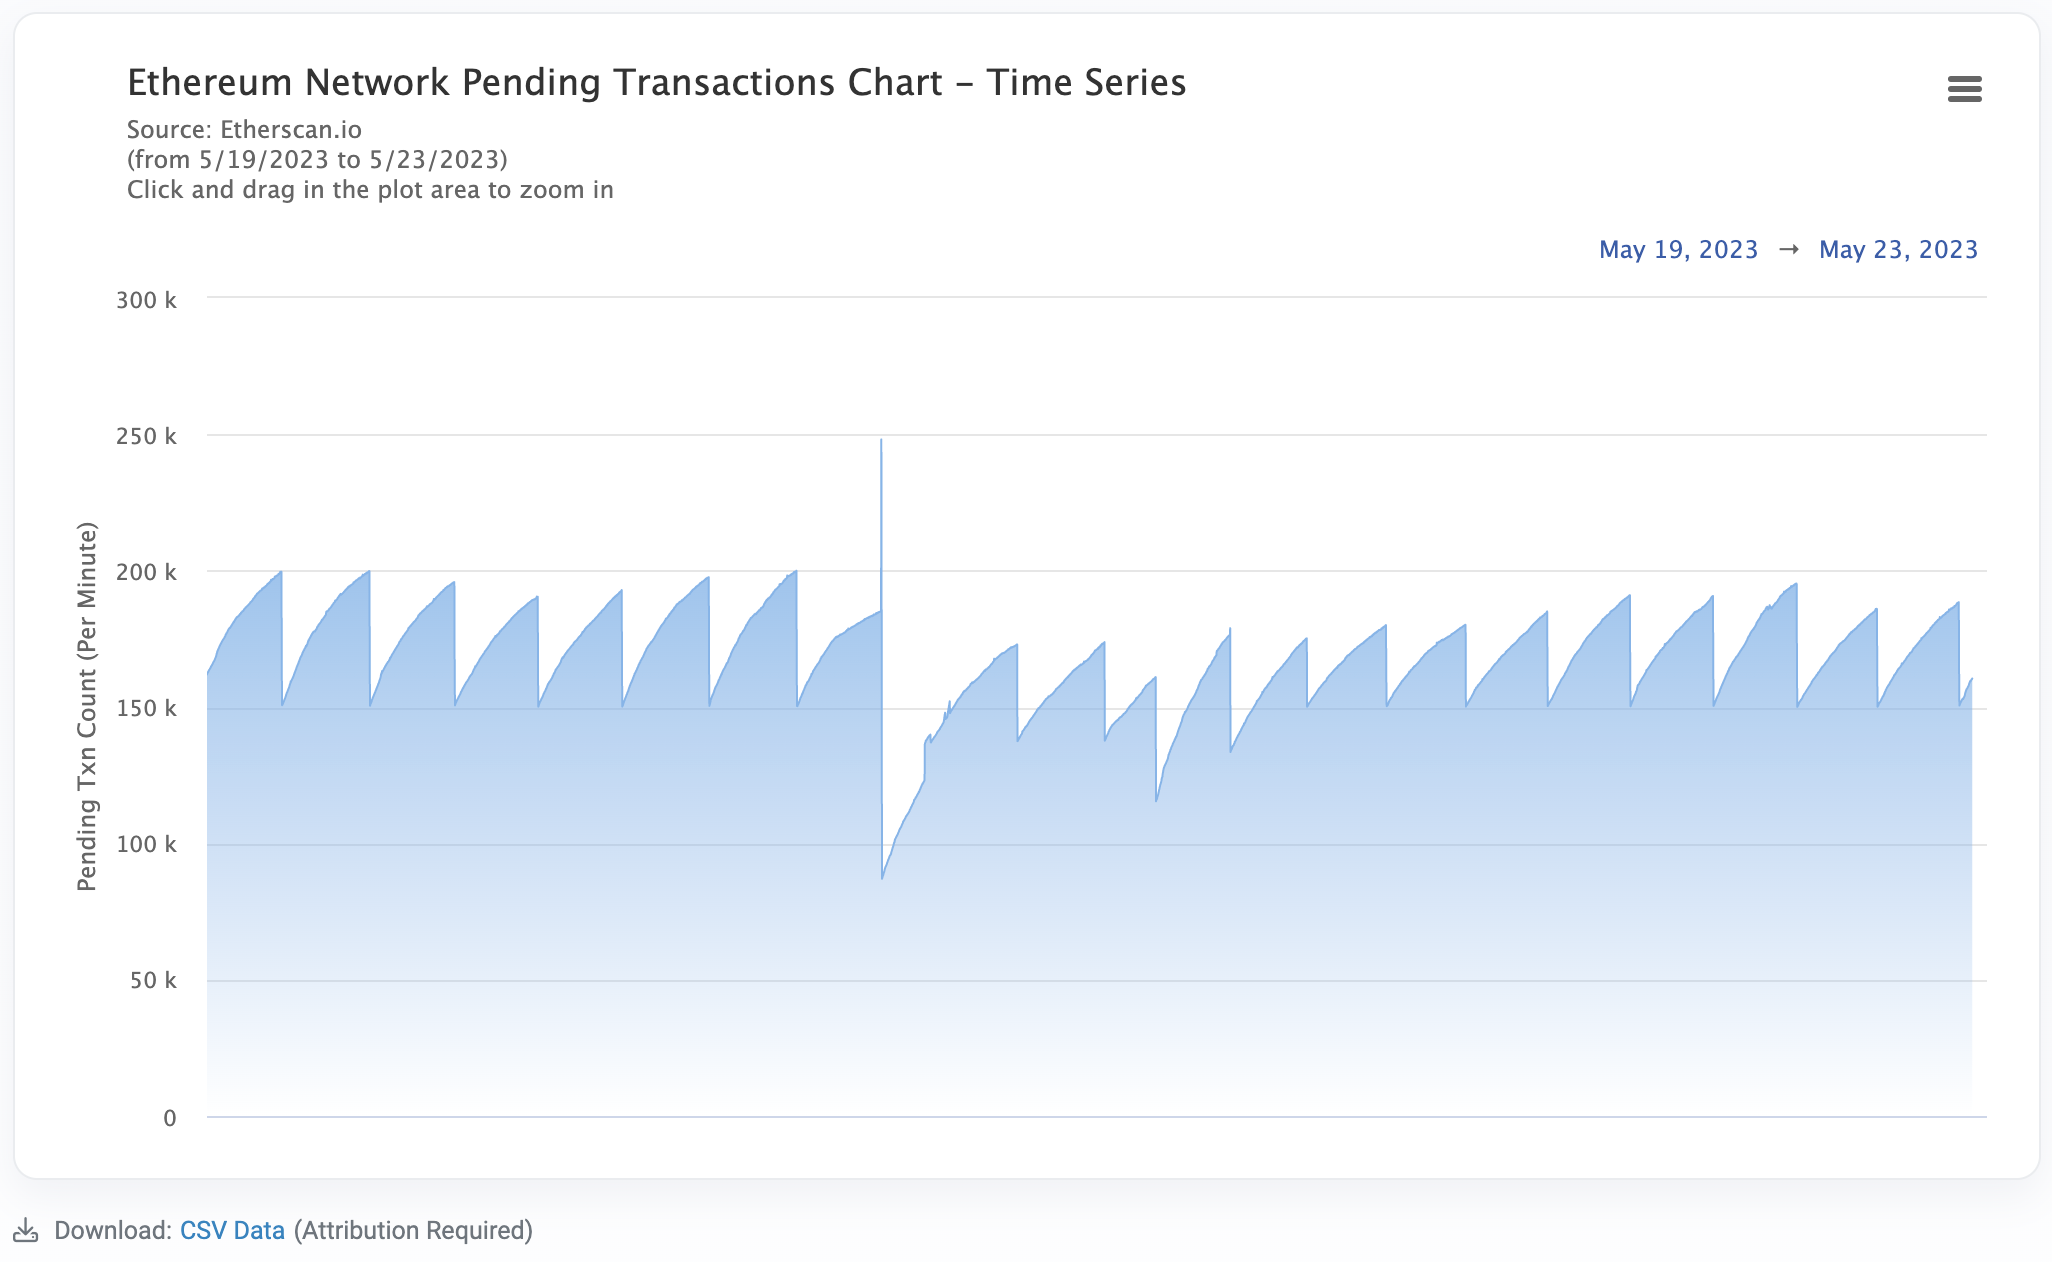
\includegraphics[width=0.48\linewidth]{images/pendchart}
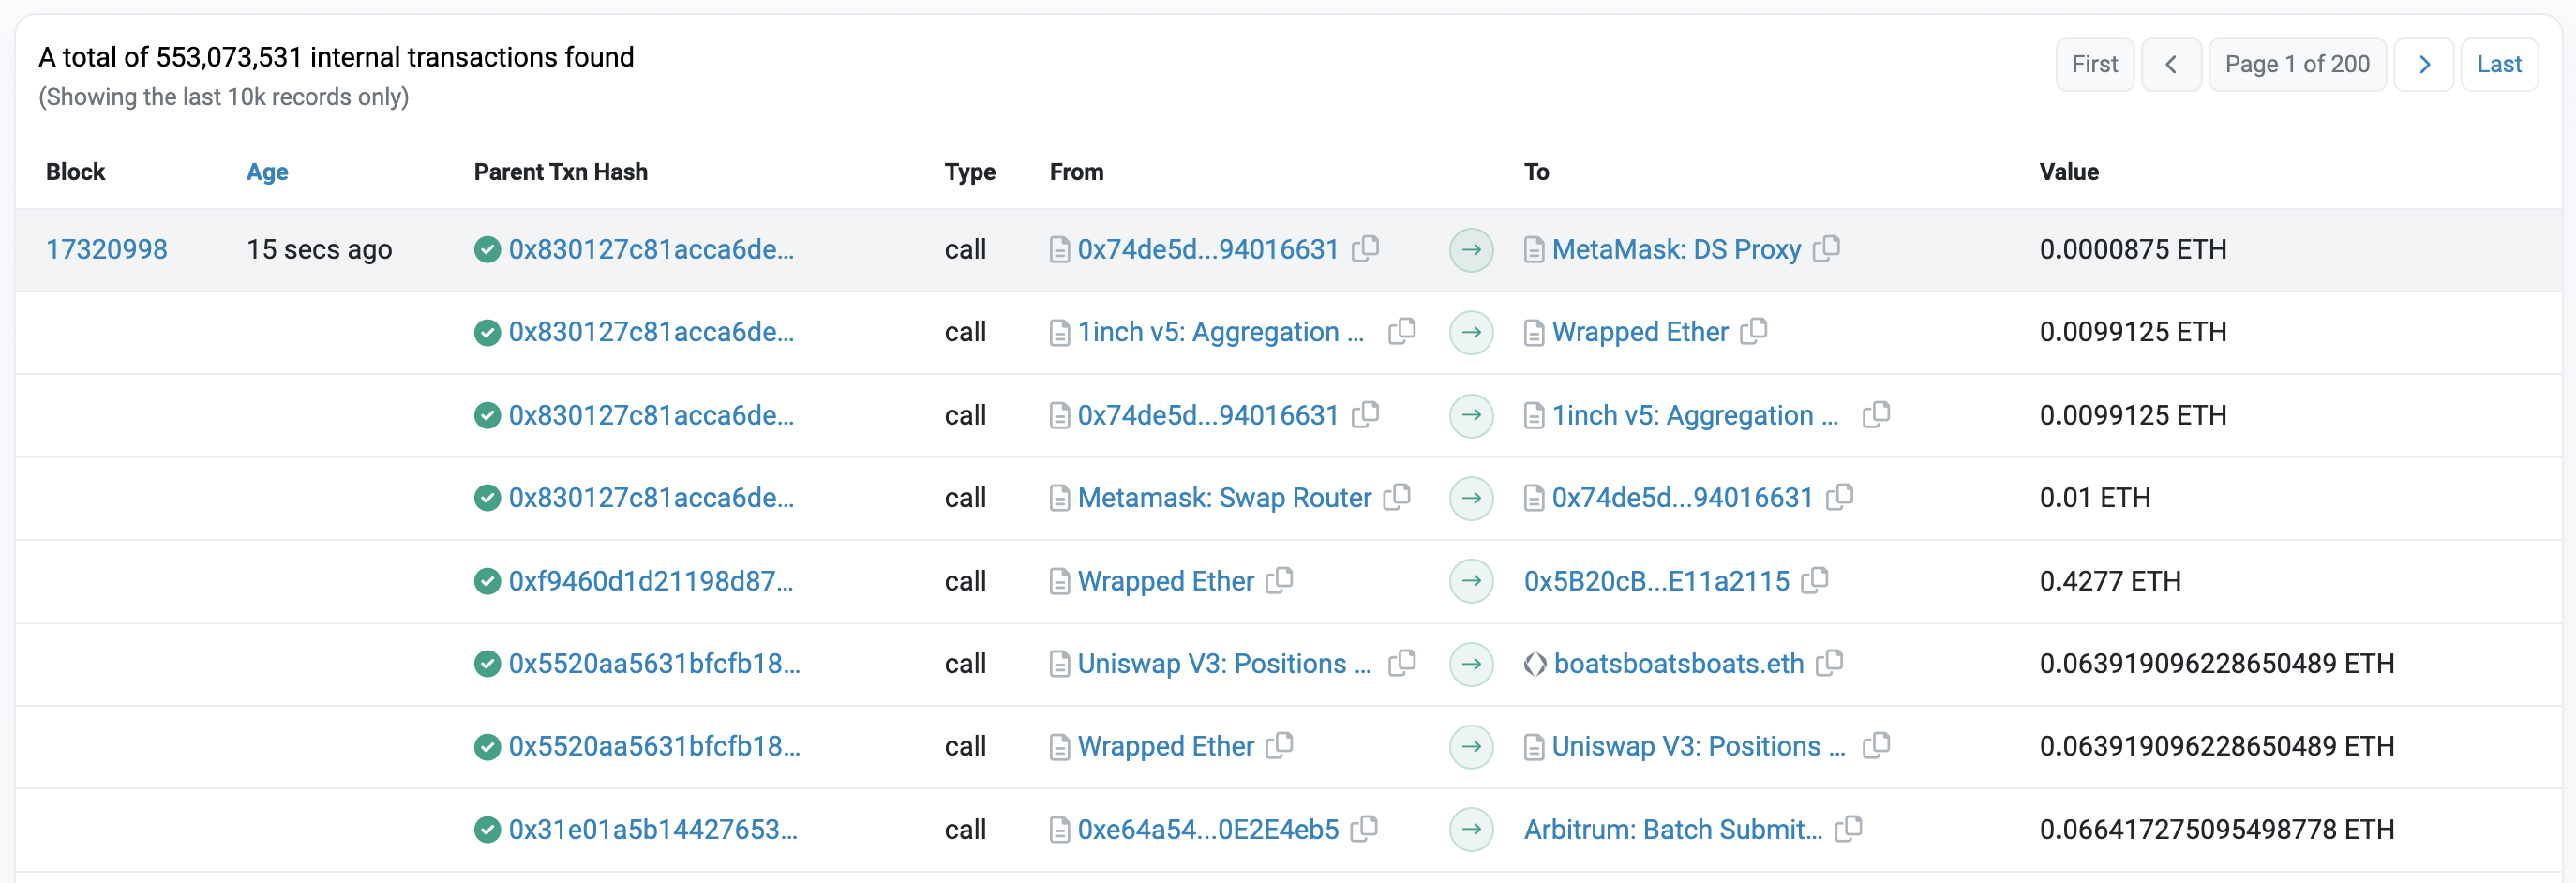
\includegraphics[width=0.48\linewidth]{images/internal} \\
(a)\hspace{160pt}        (b)\\
\caption{Chart of pending transactions (a) and contract internal transactions (b) from Etherscan (23 May 2023)}
\label{fig:pendchart}
\end{center}
\end{figure}

\begin{figure}[htbp]
\begin{center}
\includegraphics[width=0.48\linewidth]{images/deposits}
\includegraphics[width=0.48\linewidth]{images/withdrawals} \\
(a)\hspace{160pt}        (b)\\
\caption{Beacon chain deposits (a) and withdrawals (b) from Etherscan (23 May 2023)}
\label{fig:deposits}
\end{center}
\end{figure}

\begin{figure}[htbp]
\begin{center}
\includegraphics[width=0.48\linewidth]{images/blocks}
\includegraphics[width=0.48\linewidth]{images/forked} \\
(a)\hspace{160pt}        (b)\\
\caption{Details of beacon chain epochs (a) and forked blocks (b). Etherscan (23 May 2023)}
\label{fig:blocks}
\end{center}
\end{figure}

\begin{figure}[htbp]
\begin{center}
\includegraphics[width=0.48\linewidth]{images/ethscanepoch1}
\includegraphics[width=0.48\linewidth]{images/ethscanepoch} \\
(a)\hspace{160pt}        (b)\\
\caption{Details of beacon chain epochs (a) and detailed information for one epoch (b). Etherscan (7 June 2023)}
\label{fig:ethscanepoch1}
\end{center}
\end{figure}

\begin{figure}[htbp]
\begin{center}
\includegraphics[width=0.8\linewidth]{images/ethscanblk1}
\includegraphics[width=0.8\linewidth]{images/ethscanblk2} \\
\includegraphics[width=0.8\linewidth]{images/ethscanblk3} \\
\caption{Detailed information of a block, e.g. block 16766859. Etherscan (7 June 2023)}
\label{fig:ethscanblk1}
\end{center}
\end{figure}

\begin{figure}[htbp]
\begin{center}
\includegraphics[width=0.48\linewidth]{images/accounts}
\includegraphics[width=0.48\linewidth]{images/contracts} \\
(a)\hspace{160pt}        (b)\\
\caption{Top accounts by ETH balance (a) and verified contract source code (b). Etherscan (23 May 2023)}
\label{fig:accounts}
\end{center}
\end{figure}

\begin{figure}[htbp]
\begin{center}
\includegraphics[width=0.48\linewidth]{images/erc20}
\includegraphics[width=0.48\linewidth]{images/xfrs} \\
(a)\hspace{160pt}        (b)\\
\caption{Top ERC20 tokens (a) and ERC20 token transfers (b) from Etherscan (23 May 2023)}
\label{fig:erc20}
\end{center}
\end{figure}

\clearpage
\textbf{Charts and Statistics}\\
% -------------------------------------
\textit{\textbf{Market data}}
% -----------------------
\begin{figure}[htbp]
\begin{center}
\includegraphics[width=0.9\linewidth]{images/ethdaily}
\caption{Ether daily price (USD) from Etherscan, 23 May 2023}
\label{fig:ethdaily}
\end{center}
\end{figure}

\begin{figure}[htbp]
\begin{center}
\includegraphics[width=0.9\linewidth]{images/marketcap}
\caption{Ether market capitalisation from Etherscan  - select time range or zoom in on selected part of graph, hover mouse for details (as shown), 23 May 2023}
\label{fig:marketcap}
\end{center}
\end{figure}

\begin{figure}[htbp]
\begin{center}
\includegraphics[width=0.9\linewidth]{images/totcap}
\caption{Ether total supply and market capitalisation from Etherscan, 23 May 2023}
\label{fig:totcap}
\end{center}
\end{figure}

\begin{figure}[htbp]
\begin{center}
\includegraphics[width=0.9\linewidth]{images/ethgrowth}
\caption{Ether supply growth chart from Etherscan - select time range or zoom in on selected part of graph, 23 May 2023}
\label{fig:ethgrowth}
\end{center}
\end{figure}

\clearpage

\textit{\textbf{Blockchain data}}
% ------------------------------------
\begin{figure}[htbp]
\begin{center}
\includegraphics[width=0.9\linewidth]{images/ethdailytxns}
\caption{Daily transactions. Etherscan, 20 June 2023}
\label{fig:ethdailytxns}
\end{center}
\end{figure}

\begin{figure}[htbp]
\begin{center}
\includegraphics[width=0.9\linewidth]{images/ethdailyerc20}
\caption{ERC20 Daily token transfers. Etherscan, 20 June 2023}
\label{fig:ethdailyerc20}
\end{center}
\end{figure}

\begin{figure}[htbp]
\begin{center}
\includegraphics[width=0.9\linewidth]{images/ethuniqueaddr}
\caption{Chart of Ethereum unique addresses. Etherscan, 20 June 2023}
\label{fig:ethuniqueaddr}
\end{center}
\end{figure}

\begin{figure}[htbp]
\begin{center}
\includegraphics[width=0.9\linewidth]{images/ethavgblk}
\caption{Ethereum average block size. Etherscan, 20 June 2023}
\label{fig:ethavgblk}
\end{center}
\end{figure}

\begin{figure}[htbp]
\begin{center}
\includegraphics[width=0.9\linewidth]{images/ethavgtime}
\caption{Ethereum average block time. Etherscan, 20 June 2023}
\label{fig:ethavgtime}
\end{center}
\end{figure}

\begin{figure}[htbp]
\begin{center}
\includegraphics[width=0.9\linewidth]{images/ethavgas}
\caption{Ethereum average gas price. Etherscan, 20 June 2023}
\label{fig:ethavgas}
\end{center}
\end{figure}

\begin{figure}[htbp]
\begin{center}
\includegraphics[width=0.9\linewidth]{images/ethgaslim}
\caption{Ethereum average gas limit. Etherscan, 20 June 2023}
\label{fig:ethgaslim}
\end{center}
\end{figure}

\begin{figure}[htbp]
\begin{center}
\includegraphics[width=0.9\linewidth]{images/ethgasused}
\caption{Ethereum daily gas used. Etherscan, 20 June 2023}
\label{fig:ethgasused}
\end{center}
\end{figure}

\begin{figure}[htbp]
\begin{center}
\includegraphics[width=0.9\linewidth]{images/ethblkreward}
\caption{Ethereum block rewards. Etherscan, 20 June 2023}
\label{fig:ethblkreward}
\end{center}
\end{figure}

\begin{figure}[htbp]
\begin{center}
\includegraphics[width=0.9\linewidth]{images/ethblkcnt}
\caption{Ethereum block rewards. Etherscan, 20 June 2023}
\label{fig:ethblkcnt}
\end{center}
\end{figure}

\begin{figure}[htbp]
\begin{center}
\includegraphics[width=0.9\linewidth]{images/ethuncle}
\caption{Ethereum uncle count and rewards. Etherscan, 20 June 2023}
\label{fig:ethuncle}
\end{center}
\end{figure}

%\begin{figure}[htbp]
%\begin{center}
%\includegraphics[width=0.9\linewidth]{images/ethsync}
%\caption{Ethereum full node sync. Etherscan, 20 June 2023}
%\label{fig:ethsync}
%\end{center}
%\end{figure}

\begin{figure}[htbp]
\begin{center}
\includegraphics[width=0.9\linewidth]{images/ethsync}
\caption{Ethereum full node sync (default). Etherscan, 20 June 2023}
\label{fig:ethsync}
\end{center}
\end{figure}

\begin{figure}[htbp]
\begin{center}
\includegraphics[width=0.9\linewidth]{images/etharch}
\caption{Ethereum full node sync (archive). Etherscan, 20 June 2023}
\label{fig:etharch}
\end{center}
\end{figure}

\begin{figure}[htbp]
\begin{center}
\includegraphics[width=0.9\linewidth]{images/ethactiv}
\caption{Daily active Ethereum addresses. Etherscan, 20 June 2023}
\label{fig:ethactiv}
\end{center}
\end{figure}

\begin{figure}[htbp]
\begin{center}
\includegraphics[width=0.9\linewidth]{images/ethactiv20}
\caption{Daily active ERC20 addresses. Etherscan, 20 June 2023}
\label{fig:ethactiv20}
\end{center}
\end{figure}

\begin{figure}[htbp]
\begin{center}
\includegraphics[width=0.9\linewidth]{images/ethtxnfee}
\caption{Average transaction fees. Etherscan, 20 June 2023}
\label{fig:ethtxnfee}
\end{center}
\end{figure}

\begin{figure}[htbp]
\begin{center}
\includegraphics[width=0.9\linewidth]{images/ethburnt}
\caption{Daily ETH burnt. Etherscan, 20 June 2023}
\label{fig:ethburnt}
\end{center}
\end{figure}

\clearpage
\textit{\textbf{Dashboards}}
% -------------------------------
\begin{figure}[htbp]
\begin{center}
\includegraphics[width=0.9\linewidth]{images/dashboards}
\caption{Screen shot of additional dashboards that are available to complement the visualisations already shown, 23 May 2023}
\label{fig:dashboards}
\end{center}
\end{figure}


\textit{\textbf{Network data}}
% -------------------------------
\begin{figure}[htbp]
\begin{center}
\includegraphics[width=0.9\linewidth]{images/nwhash}
\caption{Network hash rate, 20 June 2023}
\label{fig:nwhash}
\end{center}
\end{figure}

\begin{figure}[htbp]
\begin{center}
\includegraphics[width=0.9\linewidth]{images/nwdiff}
\caption{Network difficulty (pre-merge), 20 June 2023}
\label{fig:nwdiff}
\end{center}
\end{figure}

\begin{figure}[htbp]
\begin{center}
\includegraphics[width=0.9\linewidth]{images/nwpendtxns}
\caption{Network pending transactions, 20 June 2023}
\label{fig:nwpendtxns}
\end{center}
\end{figure}

\begin{figure}[htbp]
\begin{center}
\includegraphics[width=0.9\linewidth]{images/nwfeetxns}
\caption{Network transaction fee, 20 June 2023}
\label{fig:nwfeetxns}
\end{center}
\end{figure}

\begin{figure}[htbp]
\begin{center}
\includegraphics[width=0.9\linewidth]{images/nwutil}
\caption{Network utilisation, 20 June 2023}
\label{fig:nwutil}
\end{center}
\end{figure}

\begin{figure}[htbp]
\begin{center}
\includegraphics[width=0.9\linewidth]{images/nodetrk1} \\
\includegraphics[width=0.9\linewidth]{images/nodetrk2} \\
\includegraphics[width=0.9\linewidth]{images/nodetrk3}
\caption{Node tracker, 20 June 2023}
\label{fig:nodetrk}
\end{center}
\end{figure}

\clearpage

\textit{\textbf{Contracts}}
% -------------------------------
\begin{figure}[htbp]
\begin{center}
\includegraphics[width=0.9\linewidth]{images/dailyverified}
\caption{Daily verified contracts - select time range or zoom in on selected part of graph, 23 May 2023}
\label{fig:dailyverified}
\end{center}
\end{figure}


\clearpage
% --------------------------------------
\subsubsection*{Dune Analytics}
% --------------------------------------
\textit{\textbf{Ethereum Staking}}
% ----------------------------------------
\begin{figure}[htbp]
\begin{center}
\includegraphics[width=\linewidth]{images/hildobby1}\\
\includegraphics[width=\linewidth]{images/hildobby2}
\caption{Dune Analytics Ethereum staking charts. @hildobby  (7 June 2023)}
\label{fig:hildobby1}
\end{center}
\end{figure}

\begin{figure}[htbp]
\begin{center}
\includegraphics[width=\linewidth]{images/hildobby3}\\
\includegraphics[width=\linewidth]{images/hildobby4}
\caption{Dune Analytics ETH inflows and outflows, ETH staked and validators. @hildobby  (7 June 2023)}
\label{fig:hildobby3}
\end{center}
\end{figure}


\begin{figure}[htbp]
\begin{center}
\includegraphics[width=\linewidth]{images/hildobby5}
\caption{Dune Analytics Recent ETH staked. @hildobby  (7 June 2023)}
\label{fig:hildobby5}
\end{center}
\end{figure}

\begin{figure}[htbp]
\begin{center}
\includegraphics[width=\linewidth]{images/hildobby6}\\
\includegraphics[width=\linewidth]{images/hildobby7}
\caption{Dune Analytics ETH staked and withdrawn by entity. @hildobby  (7 June 2023)}
\label{fig:hildobby6}
\end{center}
\end{figure}

\begin{figure}[htbp]
\begin{center}
\includegraphics[width=\linewidth]{images/hildobby8}\\
\includegraphics[width=\linewidth]{images/hildobby9}
\caption{Dune Analytics ETH staked by entity and category. @hildobby  (7 June 2023)}
\label{fig:hildobby8}
\end{center}
\end{figure}


\begin{figure}[htbp]
\begin{center}
\includegraphics[width=\linewidth]{images/hildobby10}
\caption{Dune Analytics Staking deposit market share. @hildobby  (7 June 2023)}
\label{fig:hildobby=10}
\end{center}
\end{figure}

\begin{figure}[htbp]
\begin{center}
\includegraphics[width=\linewidth]{images/hildobby11}
\caption{Dune Analytics Staker profit. @hildobby  (7 June 2023)}
\label{fig:hildobby=11}
\end{center}
\end{figure}


\clearpage
\textbf{LIDO}
% -------------
\begin{figure}[htbp]
\begin{center}
\includegraphics[width=\linewidth]{images/dunelido1}\\
\includegraphics[width=\linewidth]{images/dunelido2}
\caption{Dune Analytics Lido post Merge protocol APR dashboard by @LidoAnalytical  (7 June 2023)}
\label{fig:dunelido1}
\end{center}
\end{figure}

\begin{figure}[htbp]
\begin{center}
\includegraphics[width=\linewidth]{images/dunelido3}
\caption{Dune Analytics Lido Execution Layer rewards by @LidoAnalytical  (7 June 2023)}
\label{fig:dunelido3}
\end{center}
\end{figure}

\begin{figure}[htbp]
\begin{center}
\includegraphics[width=\linewidth]{images/dunelido4}\\
\includegraphics[width=\linewidth]{images/dunelido5}
\caption{Dune Analytics Lido MEV builders statistics by @LidoAnalytical  (7 June 2023)}
\label{fig:dunelido5}
\end{center}
\end{figure}
\noindent
\clearpage
\noindent

\textbf{Rocket Pool}
% -------------
\begin{figure}[htbp]
\begin{center}
\includegraphics[width=\linewidth]{images/dunerocket1}\\
\includegraphics[width=\linewidth]{images/dunerocket2}
\caption{Dune Analytics Rocket Pool overview by @KIV  (7 June 2023)}
\label{fig:dunerocket1}
\end{center}
\end{figure}

\begin{figure}[htbp]
\begin{center}
\includegraphics[width=\linewidth]{images/dunerocket3}
\caption{Dune Analytics Rocket Pool node operator deposits by @KIV  (7 June 2023)}
\label{fig:dunerocket3}
\end{center}
\end{figure}

\begin{figure}[htbp]
\begin{center}
\includegraphics[width=\linewidth]{images/rocketdrworm1}
\caption{Dune Analytics Rocket Pool overview by @drworm  (7 June 2023)}
\label{fig:rocketdrworm1}
\end{center}
\end{figure}

\begin{figure}[htbp]
\begin{center}
\includegraphics[width=\linewidth]{images/rocketdrworm2}
\caption{Dune Analytics Rocket Pool various statistics by @drworm  (7 June 2023)}
\label{fig:rocketdrworm2}
\end{center}
\end{figure}

\begin{figure}[htbp]
\begin{center}
\includegraphics[width=\linewidth]{images/rocketdrworm3}
\caption{Dune Analytics Rocket Pool ETH deposited \& rETH minted by @drworm  (7 June 2023)}
\label{fig:rocketdrworm3}
\end{center}
\end{figure}


\begin{figure}[htbp]
\begin{center}
\includegraphics[width=\linewidth]{images/rocketdrworm4}
\caption{Dune Analytics Rocket Pool liquid staking derivatives peg price performance by @worm  (7 June 2023)}
\label{fig:rocketdrworm4}
\end{center}
\end{figure}

\begin{figure}[htbp]
\begin{center}
\includegraphics[width=\linewidth]{images/rocketdrworm5}
\caption{Dune Analytics Rocket Pool rETH liquidity by @drworm  (7 June 2023)}
\label{fig:rocketdrworm5}
\end{center}
\end{figure}

\begin{figure}[htbp]
\begin{center}
\includegraphics[width=\linewidth]{images/rocketdrworm6}
\caption{Dune Analytics Rocket Pool rETH DEX statistics by @drworm  (7 June 2023)}
\label{fig:rocketdrworm6}
\end{center}
\end{figure}

\begin{figure}[htbp]
\begin{center}
\includegraphics[width=\linewidth]{images/rocketdrworm7}
\caption{Dune Analytics Rocket Pool rETH DEX graphs by @drworm  (7 June 2023)}
\label{fig:rocketdrworm7}
\end{center}
\end{figure}

\begin{figure}[htbp]
\begin{center}
\includegraphics[width=\linewidth]{images/rocketdrworm8}
\caption{Dune Analytics Rocket Pool node operators by @drworm  (7 June 2023)}
\label{fig:rocketdrworm8}
\end{center}
\end{figure}

\begin{figure}[htbp]
\begin{center}
\includegraphics[width=\linewidth]{images/rocketdrworm9}
\caption{Dune Analytics Rocket Pool oDAO-Reported RPL Price/RPL Staked by @drworm  (7 June 2023)}
\label{fig:rocketdrworm9}
\end{center}
\end{figure}

\begin{figure}[htbp]
\begin{center}
\includegraphics[width=\linewidth]{images/rocketdrworm10}\\
\includegraphics[width=\linewidth]{images/rocketdrworm11}
\caption{Dune Analytics Rocket Pool Minipools by @drworm  (7 June 2023)}
\label{fig:rocketdrworm10}
\end{center}
\end{figure}

\begin{figure}[htbp]
\begin{center}
\includegraphics[width=\linewidth]{images/rocketdrworm12}
\caption{Dune Analytics Rocket Pool Rocket Pool Minipools by @drworm  (7 June 2023)}
\label{fig:rocketdrworm12}
\end{center}
\end{figure}

\clearpage
\noindent

\textbf{ETH burnt}
% ------------------------------------
\begin{figure}[htbp]
\begin{center}
\includegraphics[width=\linewidth]{images/cembar1}
\caption{Dune Analytics of ETH not available for selling, i.e. ETH is burnt or staked by @cembar (6 June 2023)}
\label{fig:cembar1}
\end{center}
\end{figure}

\begin{figure}[htbp]
\begin{center}
\includegraphics[width=\linewidth]{images/cembar2}\\
\includegraphics[width=\linewidth]{images/cembar3}
\caption{Dune Analytics of total and daily ETH burnt  by @cembar (6 June 2023)}
\label{fig:cembar2}
\end{center}
\end{figure}


\clearpage

% --------------------------------------
\subsubsection*{Beaconcha.in}
% --------------------------------------
The website provides the ability to search using a variety of fields, including a public key, block number, block graffiti, proposer, slot, and epoch. Apart from the extensive information and visualisations shown here, there are several other 

\begin{figure}[htbp]
\begin{center}
\includegraphics[width=0.9\linewidth]{images/bhomepg}
\caption{Homepage of beaconcha.in showing a progress line of the slots in the current epoch with a graph of total staked Ether and active validators over the last week, from Beaconcha.in (24 May 2023)}
\label{fig:bhomepg}
\end{center}
\end{figure}

\begin{figure}[htbp]
\begin{center}
\includegraphics[width=0.9\linewidth]{images/bhomepg2}
\caption{Homepage of beaconcha.in showing the most recent epochs and blocks, from Beaconcha.in (24 May 2023)}
\label{fig:bhomepg2}
\end{center}
\end{figure}
\clearpage


\textbf{Blockchain data}
% -----------------------------
\begin{figure}[htbp]
\begin{center}
\includegraphics[width=0.9\linewidth]{images/bepochs}
\caption{Detailed information for epochs with the ability to search for a specific epoch, from Beaconcha.in (24 May 2023)}
\label{fig:bepochs}
\end{center}
\end{figure}

\begin{figure}[htbp]
\begin{center}
\includegraphics[width=0.9\linewidth]{images/bslots}
\caption{Detailed information for slots with the ability to search by block number, graffiti or proposer number, from Beaconcha.in (24 May 2023)}
\label{fig:bslots}
\end{center}
\end{figure}

\begin{figure}[htbp]
\begin{center}
\includegraphics[width=0.9\linewidth]{images/bblocks}
\caption{Detailed information of all blocks, from Beaconcha.in (24 May 2023)}
\label{fig:bblocks}
\end{center}
\end{figure}

\begin{figure}[htbp]
\begin{center}
\includegraphics[width=0.9\linewidth]{images/btxns}
\caption{Detailed information of all transactions, from Beaconcha.in (24 May 2023)}
\label{fig:btxns}
\end{center}
\end{figure}

\begin{figure}[htbp]
\begin{center}
\includegraphics[width=0.9\linewidth]{images/bmempool}
\caption{Mempool transaction details, from Beaconcha.in (24 May 2023)}
\label{fig:bmempool}
\end{center}
\end{figure}
\clearpage


\textit{\textbf{Validator data}}
% -------------------------
\begin{figure}[htbp]
\begin{center}
\includegraphics[width=0.9\linewidth]{images/bvalidators}
\caption{Overview of validators. Beaconcha.in (24 May 2023)}
\label{fig:bvalidators}
\end{center}
\end{figure}

\begin{figure}[htbp]
\begin{center}
\includegraphics[width=0.9\linewidth]{images/bslashed}
\caption{Slashed validators. Beaconcha.in (24 May 2023)}
\label{fig:bslashed}
\end{center}
\end{figure}

\begin{figure}[htbp]
\begin{center}
\includegraphics[width=0.9\linewidth]{images/bvalleader}
\caption{Validator leaderboard - default listing order is by 7day income, but it is possible to display the order by income based on 1day, 31 days or 1 year. Beaconcha.in (24 May 2023)}
\label{fig:bvalleader}
\end{center}
\end{figure}

\begin{figure}[htbp]
\begin{center}
\includegraphics[width=0.9\linewidth]{images/bdeplead}\\
\includegraphics[width=0.9\linewidth]{images/bdepleadtbl}
\caption{Leaderboard for deposits made by Ethereum addresses to the deposit contract - default order is by total amount deposited, but it is possible to display the order using any of the other columns shown in the table. Beaconcha.in (24 May 2023)}
\label{fig:bdepleadtbl}
\end{center}
\end{figure}

\begin{figure}[htbp]
\begin{center}
\includegraphics[width=0.9\linewidth]{images/bdeposits}
\caption{Visualisation of deposits since beaconchain genesis. Beaconcha.in (24 May 2023)}
\label{fig:bdeposits}
\end{center}
\end{figure}

\begin{figure}[htbp]
\begin{center}
\includegraphics[width=0.9\linewidth]{images/bdeposittbl}
\caption{Initiated deposits: table of the deposits made by validators wishing to join the beaconchain.. Beaconcha.in (24 May 2023)}
\label{fig:bdeposittbl}
\end{center}
\end{figure}

\begin{figure}[htbp]
\begin{center}
\includegraphics[width=0.48\linewidth]{images/bdeposittbltime}
\includegraphics[width=0.48\linewidth]{images/bdeposittblamount} \\
(a)\hspace{160pt}        (b)\\
\caption{Table of deposits ordered by time (a) and by amount deposited (b). Beaconcha.in (24 May 2023)}
\label{fig:bdeposittbltime}
\end{center}
\end{figure}

\begin{figure}[htbp]
\begin{center}
\includegraphics[width=0.9\linewidth]{images/bincldep}
\caption{Included deposits: table of the deposits received by the beaconchain. Beaconcha.in (24 May 2023)}
\label{fig:bincldep}
\end{center}
\end{figure}

\begin{figure}[htbp]
\begin{center}
\includegraphics[width=0.9\linewidth]{images/bwithdrawals}\\
\includegraphics[width=0.9\linewidth]{images/bwithdrawalstbl}
\caption{Histogram and table of withdrawals. Beaconcha.in (24 May 2023)}
\label{fig:bwithdrawals}
\end{center}
\end{figure}

\begin{figure}[htbp]
\begin{center}
\includegraphics[width=0.9\linewidth]{images/bblschgs}
\caption{Table displaying the BLS address changes from 0x00 credentials to 0x01. Beaconcha.in (24 May 2023)}
\label{fig:bblschgs}
\end{center}
\end{figure}

\begin{figure}[htbp]
\begin{center}
\includegraphics[width=0.9\linewidth]{images/bvaldashboard}
\caption{Validator dashboard - add the validators of interest to the search bar. In this example we added three validators: one active, one voluntary exited and one slashed validator. Beaconcha.in (24 May 2023)}
\label{fig:bvaldashboard}
\end{center}
\end{figure}

\begin{figure}[htbp]
\begin{center}
\includegraphics[width=0.9\linewidth]{images/bcorrelations}
\caption{It is possible to generate correlation visualisations between several variables. Beaconcha.in (24 May 2023)}
\label{fig:bcorrelations}
\end{center}
\end{figure}

\clearpage
\textit{\textbf{Consensus Layer Charts}}
% -------------------------------------------
\begin{figure}[htbp]
\begin{center}
\includegraphics[width=0.48\linewidth]{images/bchart1}
\includegraphics[width=0.48\linewidth]{images/bchart2} \\
(a)\hspace{160pt}        (b)\\
\caption{History of daily blocks proposed (a) and daily active validators (b) from Beaconcha.in (24 May 2023)}
\label{fig:chart1}
\end{center}
\end{figure}

\begin{figure}[htbp]
\begin{center}
\includegraphics[width=0.48\linewidth]{images/bchart3}
\includegraphics[width=0.48\linewidth]{images/bchart4} \\
(a)\hspace{160pt}        (b)\\
\caption{History of daily staked Ether (sum of all effective balances) (a) and average daily validator balance (b) from Beaconcha.in (24 May 2023)}
\label{fig:chart3}
\end{center}
\end{figure}

\begin{figure}[htbp]
\begin{center}
\includegraphics[width=0.48\linewidth]{images/bchart5}
\includegraphics[width=0.48\linewidth]{images/bchart6} \\
(a)\hspace{160pt}        (b)\\
\caption{Network liveness (measures how far the last finalised epoch is behind the head epoch. The protocol allows epochs to be finalised after 2 epochs) (a) and participation rate (measures how many of the validators expected to attest to blocks are actually doing so) (b) from Beaconcha.in (24 May 2023)}
\label{fig:chart5}
\end{center}
\end{figure}

\begin{figure}[htbp]
\begin{center}
\includegraphics[width=0.48\linewidth]{images/bchart7}
\includegraphics[width=0.48\linewidth]{images/bchart8} \\
(a)\hspace{160pt}        (b)\\
\caption{Stake effectiveness (measures the relation between the sum if all effective balances and the sum of all balances. 100\% stake effectiveness means that 100\% of the locked ETH is used for staking) (a) and balance distribution (b) from Beaconcha.in (24 May 2023)}
\label{fig:chart7}
\end{center}
\end{figure}

\begin{figure}[htbp]
\begin{center}
\includegraphics[width=0.48\linewidth]{images/bchart9a}
\includegraphics[width=0.48\linewidth]{images/bchart9} \\
(a)\hspace{160pt}        (b)\\
\caption{Effective balance distribution showing information on the lowest balance - 0.04ETH (a) and for 32 ETH (b) from Beaconcha.in (24 May 2023)}
\label{fig:chart9}
\end{center}
\end{figure}

\begin{figure}[htbp]
\begin{center}
\includegraphics[width=0.48\linewidth]{images/bchart10}
\includegraphics[width=0.48\linewidth]{images/bchart11a} \\
(a)\hspace{160pt}        (b)\\
\caption{Income distribution for the last 365 days (a) and Daily amount of deposited ETH on the consensus layer (b) from Beaconcha.in (24 May 2023)}
\label{fig:chart10}
\end{center}
\end{figure}


\begin{figure}[htbp]
\begin{center}
\includegraphics[width=0.48\linewidth]{images/bchart11b}
\includegraphics[width=0.48\linewidth]{images/bchart12a} \\
(a)\hspace{160pt}        (b)\\
\caption{Daily amount of deposited ETH on the execution layer  (a) and a graffiti word cloud of the 25 most occurring graffities (b) from Beaconcha.in (24 May 2023)}
\label{fig:chart11}
\end{center}
\end{figure}

\begin{figure}[htbp]
\begin{center}
\includegraphics[width=0.48\linewidth]{images/bchart13a}
\includegraphics[width=0.48\linewidth]{images/bchart13b} \\
(a)\hspace{160pt}        (b)\\
\caption{Validator distribution by staking pool  (a) and honing in on the proportion of validators not allocated to a known staking pool  (b) from Beaconcha.in (24 May 2023)}
\label{fig:chart13a}
\end{center}
\end{figure}

\begin{figure}[htbp]
\begin{center}
\includegraphics[width=0.48\linewidth]{images/bchart13c}
\includegraphics[width=0.48\linewidth]{images/bchart13d} \\
(a)\hspace{160pt}        (b)\\
\caption{Validator distribution by staking pool showing the Lido pool (a) and Rocketpool (b) from Beaconcha.in (24 May 2023)}
\label{fig:chart13c}
\end{center}
\end{figure}

\begin{figure}[htbp]
\begin{center}
\includegraphics[width=0.48\linewidth]{images/bchart14a}
\includegraphics[width=0.48\linewidth]{images/bchart14b} \\
(a)\hspace{160pt}        (b)\\
\caption{Historical pool performance (a) and honing in on Rocketpool preformance (b) from Beaconcha.in (24 May 2023)}
\label{fig:chart14}
\end{center}
\end{figure}

\begin{figure}[htbp]
\begin{center}
\includegraphics[width=0.48\linewidth]{images/bchart15}
\includegraphics[width=0.48\linewidth]{images/bchart16} \\
(a)\hspace{160pt}        (b)\\
\caption{Daily amounts of withdrawals (a) and slot visualisation (click on the diagram for more detail) (b) from Beaconcha.in (24 May 2023)}
\label{fig:chart15}
\end{center}
\end{figure}
\clearpage

\textit{\textbf{Execution layer charts}}
% -------------------------------------
\begin{figure}[htbp]
\begin{center}
\includegraphics[width=0.48\linewidth]{images/bchart17}
\includegraphics[width=0.48\linewidth]{images/bchart18} \\
(a)\hspace{160pt}        (b)\\
\caption{Evolution of total ether supply (a) and of the Ethereum market capitilisation (b) from Beaconcha.in (24 May 2023)}
\label{fig:chart17}
\end{center}
\end{figure}

\begin{figure}[htbp]
\begin{center}
\includegraphics[width=0.48\linewidth]{images/bchart19}
\includegraphics[width=0.48\linewidth]{images/bchart20} \\
(a)\hspace{160pt}        (b)\\
\caption{The average amount of gas used by blocks per day (a) and the evolution of the total amount of Ether burned with EIP1559 (b) from Beaconcha.in (24 May 2023)}
\label{fig:chart19}
\end{center}
\end{figure}

\begin{figure}[htbp]
\begin{center}
\includegraphics[width=0.48\linewidth]{images/bchart21}
\includegraphics[width=0.48\linewidth]{images/bchart22} \\
(a)\hspace{160pt}        (b)\\
\caption{The daily total amount of gas used  (a) and the number of blocks produced daily (b) from Beaconcha.in (24 May 2023)}
\label{fig:chart21}
\end{center}
\end{figure}

\begin{figure}[htbp]
\begin{center}
\includegraphics[width=0.48\linewidth]{images/bchart23}
\includegraphics[width=0.48\linewidth]{images/bchart24} \\
(a)\hspace{160pt}        (b)\\
\caption{Average time between blocks over the last 24 hours (a) and the evolution of the average block gas limit (b) from Beaconcha.in (24 May 2023)}
\label{fig:chart23}
\end{center}
\end{figure}

\begin{figure}[htbp]
\begin{center}
\includegraphics[width=0.48\linewidth]{images/bchart25}
\includegraphics[width=0.48\linewidth]{images/bchart26} \\
(a)\hspace{160pt}        (b)\\
\caption{Evolution of the average utilisation of Ethereum blocks (a) and the total number of transactions per day (b) from Beaconcha.in (24 May 2023)}
\label{fig:chart25}
\end{center}
\end{figure}

\clearpage
% --------------------------------------
\subsubsection*{Mevboost.pics}
% --------------------------------------
\textbf{General Dashboard} \\
% ----------------------------------
\begin{figure}[htbp]
\begin{center}
\includegraphics[width=0.9\linewidth]{images/mevhome1}
\caption{General Dashboard - summary statistics. Mevboost.pics.(29 May 2023)}
\label{fig:mevhome1}
\end{center}
\end{figure}

\begin{figure}[htbp]
\begin{center}
\includegraphics[width=0.9\linewidth]{images/mevhome2}
\caption{General Dashboard - slot share, daily gas and MEV revenue with the option of choosing different time periods. Mevboost.pics.(29 May 2023)}
\label{fig:mevhome2}
\end{center}
\end{figure}

\begin{figure}[htbp]
\begin{center}
\includegraphics[width=0.9\linewidth]{images/mevhome3}
\caption{General Dashboard -  Average MEV-Boost payments per block - choose between 14 days, 60 days, 6 months or since the merge. Mevboost.pics.(29 May 2023)}
\label{fig:mevhome3}
\end{center}
\end{figure}

\begin{figure}[htbp]
\begin{center}
\includegraphics[width=0.9\linewidth]{images/mevhome4}
\caption{General Dashboard - MEV-Boost block flow. Select to display all builders, only builders active in the past 7 days, excluding small builders, or choose  a builder from the available list. Mevboost.pics.(29 May 2023)}
\label{fig:mevhome4}
\end{center}
\end{figure}
\clearpage

\textbf{Relays Dashboard}
% ----------------------------------
\begin{figure}[htbp]
\begin{center}
\includegraphics[width=0.85\linewidth]{images/mevrelay1}
\caption{Relay Dashboard - MEV-Boost relay market (last 14 days) and total cumulative slot share (select from time ranges: 7 days, 1 month, since merge). Mevboost.pics.(29 May 2023)}
\label{fig:mevrelay1}
\end{center}
\end{figure}

\begin{figure}[htbp]
\begin{center}
\includegraphics[width=0.9\linewidth]{images/mevrelay2}
\caption{Relay Dashboard - Slots per hour (last 7 days) and bids received (last 48 hours). Mevboost.pics.(29 May 2023)}
\label{fig:mevrelay2}
\end{center}
\end{figure}

\begin{figure}[htbp]
\begin{center}
\includegraphics[width=0.9\linewidth]{images/mevrelay3}
\caption{Relay Dashboard - MEV-Boost payments (select from last 48 hours, 7 days, 30 days or 6 months) and average MEV-Boost proposer payment per block (either for the last 6 months or since the merge). Mevboost.pics.(29 May 2023)}
\label{fig:mevrelay3}
\end{center}
\end{figure}

\begin{figure}[htbp]
\begin{center}
\includegraphics[width=0.9\linewidth]{images/mevrelay4}
\caption{Blocks per relay. Press play to see the visualisation of the blocks per relayer change over time. Mevboost.pics.(29 May 2023)}
\label{fig:mevrelay4}
\end{center}
\end{figure}

\clearpage
\textbf{Builders Dashboard} 
% ----------------------------------
\begin{figure}[htbp]
\begin{center}
\includegraphics[width=0.85\linewidth]{images/mevbuilder1}
\caption{Builders Dashboard - MEV-Boost builder market for the last 14 days  and total cumulative slot share (select from time ranges: 7 days, 1 month, since merge). Mevboost.pics.(29 May 2023)}
\label{fig:mevbuilder1}
\end{center}
\end{figure}

\begin{figure}[htbp]
\begin{center}
\includegraphics[width=0.9\linewidth]{images/mevbuilder2}
\caption{Builders Dashboard - Slots per hour (last 7 days) and bids submitted  for the last 24 hours (select all builders, or one from the list provided). Mevboost.pics.(29 May 2023)}
\label{fig:mevbuilder2}
\end{center}
\end{figure}

\begin{figure}[htbp]
\begin{center}
\includegraphics[width=0.9\linewidth]{images/mevbuilder3}
\caption{Builders Dashboard - MEV-Boost payments (select from 48 hours, 7 days, 30 days, or 6 months) and timing of the successful bids (select from all relays, or from the list provided). Mevboost.pics.(29 May 2023)}
\label{fig:mevbuilder3}
\end{center}
\end{figure}

\begin{figure}[htbp]
\begin{center}
\includegraphics[width=0.9\linewidth]{images/mevbuilder4}
\caption{Builders Dashboard - Average MEV-Boost payments per block (select time range of last 6 months, or since merge) and builders overview of the last 14 days, ordered by the total number of blocks. Mevboost.pics.(29 May 2023)}
\label{fig:mevbuilder4}
\end{center}
\end{figure}


\clearpage
\textbf{Validators Dashboard} \\
% ----------------------------------
\begin{figure}[htbp]
\begin{center}
\includegraphics[width=0.85\linewidth]{images/mevvalidator1}
\caption{Validators Dashboard - MEV-Boost total validator market for the last 14 days  and total cumulative slot share (select from time ranges: 7 days, 1 month, since merge). Mevboost.pics.(29 May 2023)}
\label{fig:mevvalidator1}
\end{center}
\end{figure}

\begin{figure}[htbp]
\begin{center}
\includegraphics[width=0.9\linewidth]{images/mevvalidator2}
\caption{Validators Dashboard - Slots per hour (last 7 days) and blocks per validator: press play to see the visualisation of the blocks per validator change over time.. Mevboost.pics.(29 May 2023)}
\label{fig:mevvalidator2}
\end{center}
\end{figure}

\begin{figure}[htbp]
\begin{center}
\includegraphics[width=0.9\linewidth]{images/mevvalidator3}
\caption{Validators Dashboard - MEV-Boost payments (select from time ranges: 48 hours, 7 days, 30 days or 6 months) and cumulative total of Lido node operator slot share (select time range: 7 days, 1 month or since merge). Mevboost.pics.(29 May 2023)}
\label{fig:mevvalidator3}
\end{center}
\end{figure}

\begin{figure}[htbp]
\begin{center}
\includegraphics[width=0.9\linewidth]{images/mevvalidator4}
\caption{Validators Dashboard - Validators overview with Staker/Validator, number of validators and number of blocks proposed by the staking entity since the merge. Mevboost.pics.(29 May 2023)}
\label{fig:mevvalidator4}
\end{center}
\end{figure}

\begin{figure}[htbp]
\begin{center}
\includegraphics[width=0.9\linewidth]{images/mevboostrawdata}
\caption{Raw data can be downloaded from Mevboost.pics. Currently only the first dataset is available for download. (29 May 2023). The public key mapping dataset is now also available and will be updated daily (30 May 2023)}
\label{fig:mevboostrawdata}
\end{center}
\end{figure}

\clearpage
% --------------------------------------
\subsubsection*{Metrika}
% --------------------------------------
\textbf{Withdrawals}
% ------------------------
\begin{figure}[htbp]
\begin{center}
\includegraphics[width=0.9\linewidth]{images/metrika1}
\caption{Details will be displayed when a withdrawal address is entered. Metrika. (21 June 2023). }
\label{fig:metrika1}
\end{center}
\end{figure}

\begin{figure}[htbp]
\begin{center}
\includegraphics[width=0.9\linewidth]{images/metrika2}
\caption{Network level statistics. Metrika. (21 June 2023). }
\label{fig:metrika2}
\end{center}
\end{figure}

\begin{figure}[htbp]
\begin{center}
\includegraphics[width=0.9\linewidth]{images/metrika3}
\caption{Activation queue. Metrika. (21 June 2023). }
\label{fig:metrika3}
\end{center}
\end{figure}

\begin{figure}[htbp]
\begin{center}
\includegraphics[width=0.9\linewidth]{images/metrika4}
\caption{Circulating ETH supply (amount of ETH on the Execution Layer), net change of supply (ETH withdrawn - ETH burned - ETH deposited). Metrika. (21 June 2023). }
\label{fig:metrika4}
\end{center}
\end{figure}

\begin{figure}[htbp]
\begin{center}
\includegraphics[width=0.9\linewidth]{images/metrika5}
\caption{Average withdrawal split by withdrawal type: partial, exited or slashed, credential changes, no. of withdrawals per block.  Metrika. (21 June 2023). }
\label{fig:metrika5}
\end{center}
\end{figure}

\begin{figure}[htbp]
\begin{center}
\includegraphics[width=0.9\linewidth]{images/metrika6}
\caption{Average stake and active validators, and largest total withdrawals for a withdrawal address, split by withdrawal type.  Metrika. (21 June 2023). }
\label{fig:metrika6}
\end{center}
\end{figure}

\clearpage
% --------------------------------------
\subsubsection*{teku-besu-ohio-mainnet-archive-01}
% --------------------------------------

We are able to retrieve some rich data from the archive node \texttt{teku-besu-ohio-mainnet-archive-01} using API endpoints. For example, the data of the validators retrieved according to their status (as seen in the call statement)  includes the \textit{validator index, balance, effective balance, slashed flag, activation eligibility epoch, activation epoch, exit epoch and withdraw-able epoch}
\begin{itemize}
\item \texttt{/eth/v1/beacon/states/finalized/validators?status=`active'} \\
For each of the entries the sub-status is listed, i.e. `active\_ongoing', `active\_exiting', or `active\_slashed'. Alternatively a call can be made directly for one of these sub-statuses, e.g. \\
 \texttt{/eth/v1/beacon/states/finalized/validators?status=`active\_ongoing'}
\item \texttt{/eth/v1/beacon/states/finalized/validators?status=`pending'}\\
The two sub-statuses are: `pending\_initialized' and `pending\_queued'. \\
In a similar manner to the above sub-status call, we could run a query to extract only a specific sub-status:\\
\texttt{/eth/v1/beacon/states/finalized/validators?status=`pending\_initialized'}
\item \texttt{/eth/v1/beacon/states/finalized/validators?status=`exited'} \\
Exited status also has two sub-statuses that can be called directly: exited\_unslashed and `exited\_slashed'
\item \texttt{/eth/v1/beacon/states/finalized/validators?status=`withdrawal'} \\
Withdrawal has two substatuses: `withdrawal\_possible' and `withdrawal\_done', which can be called directly.
\end{itemize}
\clearpage

\textbf{Graphs of validator data}
% -------------------------------------------
 \begin{figure}[htbp]
\begin{center}
\includegraphics[width=\linewidth]{images/daily_validator_plot_230607}             % Note: Within images, no need to use \_ for _
\caption{Number of validators added daily}
\label{fig:dailyvalidator1}
\end{center}
\end{figure} 

\begin{figure}[htbp]
\begin{center}
\includegraphics[width=\linewidth]{images/daily_validator_plot_no_genesis_no_smoothing_230607}             % Note: Within images, no need to use \_ for _
\caption{Number of validators added daily, excluding genesis}
\label{fig:dailyvalidator2}
\end{center}
\end{figure}

\begin{figure}[htbp]
\begin{center}
\includegraphics[width=\linewidth]{images/daily_validator_plot_no_genesis_pt_no_smoothing_230607}             % Note: Within images, no need to use \_ for _
\caption{Number of validators added daily, excluding genesis}
\label{fig:dailyvalidator3}
\end{center}
\end{figure}

\begin{figure}[htbp]
\begin{center}
\includegraphics[width=\linewidth]{images/cumulative_validator_plot_230607}
\caption{Cumulative total of validators added \& activated}
\label{fig:cumulativevalidators}
\end{center}
\end{figure}


 \begin{figure}[htbp]
\begin{center}
\includegraphics[width=\linewidth]{images/cumulative_validator_plot_with_regression_line_230607}
\caption{Cumulative total of validators added \& activated with regression line fitted}
\label{fig:cumulativevalidatorsregression}
\end{center}
\end{figure}

\clearpage

\section{Bibliography}
% -----------------------------
\nocite{*}
\bibliographystyle{eptcs}
\bibliography{references}

\end{document}
